\documentclass[twoside, a4paper, 11pt]{book}
% ------------------------------------------------------------------------------
% Packages
% ------------------------------------------------------------------------------
\usepackage[ddmmyyyy]{datetime}
\usepackage[T1]{fontenc}
\usepackage[utf8]{inputenc}

% Page setting
\usepackage[explicit]{titlesec}
\usepackage{sectsty}
\usepackage{fancyhdr}
\usepackage[title, titletoc]{appendix}

% Fonts
\usepackage{kpfonts}
\usepackage{amsmath}
\usepackage{amssymb}
\usepackage{dsfont}
\usepackage{pifont}

% Graphics and colors
\usepackage{graphicx}
\usepackage{xcolor}
\usepackage{import}

\definecolor{myred}{RGB}{150,0,0}
\definecolor{mygreen}{RGB}{0,150,0}
\definecolor{myblue}{RGB}{0, 101, 189}
\definecolor{myyellow}{RGB}{220, 206, 0}
\definecolor{myorange}{RGB}{255, 153, 51}
\definecolor{mycyan}{RGB}{51, 204, 204}
\definecolor{mypurple}{RGB}{204, 0, 153}

\newcommand{\doccol}{\color{myblue}}

% Hyperrefs
\usepackage[
  pdfusetitle,
  unicode = true,
  bookmarks = true,
  bookmarksnumbered = false,
  bookmarksopen = true,
  breaklinks = false,
  pdfborderstyle = {},
  backref = false,
  colorlinks = true,
  linkcolor = myblue,
  urlcolor = myred,
  citecolor = mygreen,
]{hyperref}


% Captions
\usepackage{caption}

\captionsetup[figure]{position = bottom}
\captionsetup[table]{position = bottom}

% Tables, Algs ...
\usepackage{enumitem}
\usepackage{algorithm}
\usepackage{algorithmicx}
\usepackage{algpseudocode}
\usepackage{booktabs}
\usepackage{nicematrix}

\renewcommand{\arraystretch}{1.5}

\newcommand{\headercol}{myblue!20}
\newcommand{\rowcol}{myblue!10}

% Math
\usepackage{nicefrac}
\usepackage{bm}
\usepackage{thm-restate}
\usepackage{optidef}
\usepackage{xspace}

% Theorems
\usepackage[framemethod=TikZ]{mdframed}
\usepackage{amsthm}
\usepackage{xifthen}

% Tikz and pfgplots
\usepackage{tikz}
\usepackage{pgfplots}
\usepackage{pgfplotstable}

\usetikzlibrary{shapes}
\usetikzlibrary{arrows}
\usetikzlibrary{automata}
\usetikzlibrary{positioning}
\usetikzlibrary{calc}
\usetikzlibrary{intersections}

\pgfplotsset{compat=newest}
\usepgfplotslibrary{groupplots}
\usepgfplotslibrary{fillbetween}

\tikzstyle{line_node} = [line width=1pt, rounded corners, color=black, ->]
\tikzstyle{line_cv} = [line width=3pt, color=mygreen, line cap=round]

% Tmp
\usepackage[color=myred!50]{todonotes}

% ------------------------------------------------------------------------------
% Math declarations
% ------------------------------------------------------------------------------
\newcommand{\Brac}[2][r]{%
  \ifx r#1 \left(       #2 \right)       \else
  \ifx c#1 \left\{      #2 \right\}      \else
  \ifx s#1 \left[       #2 \right]       \else
  \ifx v#1 \left\vert   #2 \right\vert   \else
  \ifx a#1 \left\langle #2 \right\rangle \else
  \ifx t#1 \left\lceil  #2 \right\rceil  \else
  \ifx b#1 \left\lfloor #2 \right\rfloor \else
  \ifx n#1 \left\|      #2 \right\|      \else
  \mathrm{Illegal~option}%
  \fi\fi\fi\fi\fi\fi\fi\fi
}

\newcommand{\clip}[4][s]{
  \ifx s#1 \mathrm{clip}_{\Brac[s]{#2,\; #3}}\Brac{#4} \else
  \ifx u#1 \mathrm{clip}_{\left[#2,\; #3\right)}\Brac{#4} \else
  \ifx l#1 \mathrm{clip}_{\left(#2,\; #3\right]}\Brac{#4} \else
  \mathrm{Illegal~option}%
  \fi\fi\fi
}

\DeclareMathOperator*{\argmax}{arg\,max}

\newcommand{\yesmark}{\textcolor{mygreen}{\ding{51}}}%
\newcommand{\nomark}{\textcolor{myred}{\ding{55}}}
\newcommand{\good}[1]{\textcolor{mygreen}{#1}}
\newcommand{\bad}[1]{\textcolor{myred}{#1}}

\newcommand{\R}{\mathbb{R}}
\newcommand{\N}{\mathbb{N}}
\newcommand{\X}{\mathbb{X}}

\newcommand{\I}{\mathcal{I}}
\newcommand{\Itil}{\tilde{\mathcal{I}}}
\newcommand{\Ineg}{\I_{-}}
\newcommand{\Ipos}{\I_{+}}

\newcommand{\Imb}{\I_{\text{mb}}}
\newcommand{\Imbneg}{\I_{\text{mb},-}}
\newcommand{\Imbpos}{\I_{\text{mb},+}}

\newcommand{\indmax}{j^{\star}}
\newcommand{\indmaxmb}{j^{\star}_{\text{mb}}}

\newcommand{\nall}{n}
\newcommand{\nneg}{n_{-}}
\newcommand{\npos}{n_{+}}
\newcommand{\ntil}{\tilde{n}}

\newcommand{\nmb}{n_{\text{mb}}}
\newcommand{\nmbneg}{n_{\text{mb},-}}
\newcommand{\nmbpos}{n_{\text{mb},+}}

\newcommand{\K}{\mathbb{K}}
\newcommand{\Kall}{\K^{\pm}}
\newcommand{\Kneg}{\K^{-}}

\newcommand{\alphak}{\alpha_{\hat{k}}}
\newcommand{\alphal}{\alpha_{\hat{l}}}
\newcommand{\betak}{\beta_{\hat{k}}}
\newcommand{\betal}{\beta_{\hat{l}}}

\newcommand{\norm}[1]{\Brac[n]{#1}}
\newcommand{\abs}[1]{|#1|}
\newcommand{\inner}[2]{\Brac[a]{#1, \; #2}}
\newcommand{\dd}[1]{\mathop{}\!\mathrm{d}#1}

\newcommand{\Iverson}[1]{\mathds{1}_{\Brac[s]{#1}}}

\newcommand{\EE}{\mathbb{E}}
\newcommand{\PP}{\mathbb{P}}
\newcommand{\bias}{\operatorname{bias}}

\newcommand{\Matrix}[1]{\begin{pmatrix} #1 \end{pmatrix}}
\newcommand{\Set}[2]{\Brac[c]{#1 \; \middle\vert \; #2}}
\newcommand{\domain}{\operatorname*{dom}}

\newcommand{\repeatloop}{\texttt{repeat}\xspace}
\newcommand{\forloop}{\texttt{for}\xspace}

\newcommand{\vecab}{\Matrix{\bm{\alpha} \\ \bm{\beta}}}

% models
\newcommand{\AccatTop}{\emph{Accuracy at the Top}\xspace}
\newcommand{\TopPush}{\emph{TopPush}\xspace}
\newcommand{\TopPushK}{\emph{TopPushK}\xspace}
\newcommand{\tauFPL}{{\emph{$\tau$-FPL}}\xspace}
\newcommand{\TopMeanK}{\emph{TopMeanK}\xspace}
\newcommand{\PatMat}{\emph{Pat}\&\emph{Mat}\xspace}
\newcommand{\PatMatNP}{{\emph{Pat}\&\emph{Mat-NP}}\xspace}
\newcommand{\Grill}{\emph{Grill}\xspace}
\newcommand{\GrillNP}{\emph{Grill-NP}\xspace}
\newcommand{\DeepTopPush}{\emph{DeepTopPush}\xspace}
\newcommand{\TFCO}{\emph{TFCO}\xspace}
\newcommand{\APPerf}{\emph{Ap-Perf}\xspace}
\newcommand{\BaseLine}{\emph{BinCross}\xspace}
\newcommand{\SVM}{\emph{SVM}\xspace}

% counts and rates
\DeclareMathOperator{\tp}{tp}
\DeclareMathOperator{\tn}{tn}
\DeclareMathOperator{\fp}{fp}
\DeclareMathOperator{\fn}{fn}
\DeclareMathOperator{\tpr}{tpr}
\DeclareMathOperator{\tnr}{tnr}
\DeclareMathOperator{\fpr}{fpr}
\DeclareMathOperator{\fnr}{fnr}

\DeclareMathOperator{\tps}{\overline{tp}}
\DeclareMathOperator{\tns}{\overline{tn}}
\DeclareMathOperator{\fps}{\overline{fp}}
\DeclareMathOperator{\fns}{\overline{fn}}

\DeclareMathOperator{\accuracy}{acc}
\DeclareMathOperator{\baccuracy}{bacc}
\DeclareMathOperator{\precision}{precision}
\DeclareMathOperator{\recall}{recall}
\DeclareMathOperator{\pratrec}{Precision@Recall}
\DeclareMathOperator{\postop}{pos@top}

\newcommand{\tpratk}{\operatorname{TPR@}K}
\newcommand{\tpratfpr}{\operatorname{TPR@}\tau}
\newcommand{\auroc}{\operatorname{AUROC}}

\usepackage{geometry}
\geometry{
  verbose,
  marginparwidth = 0.5cm,
  tmargin = 2.5cm,
  bmargin = 2.5cm,
  lmargin = 3cm,
  rmargin = 2cm,
  headheight = 1cm,
  headsep = 0.5cm,
  footskip = 1cm
}

% ------------------------------------------------------------------------------
% Math
% ------------------------------------------------------------------------------
\let\originalleft\left
\let\originalright\right
\renewcommand{\left}{\mathopen{}\mathclose\bgroup\originalleft}
\renewcommand{\right}{\aftergroup\egroup\originalright}

% ------------------------------------------------------------------------------
% Theorems
% ------------------------------------------------------------------------------
\mdfdefinestyle{theoremstyle}{
  outerlinewidth = 2,
  roundcorner = 1pt,
  linecolor = myblue!50,
  linewidth = 1pt,
  frametitlerule = true,
  frametitlebackgroundcolor = myblue!50,
  skipabove = 5pt,
  skipbelow = 5pt,
}

\newmdtheoremenv[style = theoremstyle]{thm}{Theorem}[chapter]
\mdtheorem[style = theoremstyle]{theorem}[thm]{Theorem}
\mdtheorem[style = theoremstyle]{lemma}[thm]{Lemma}
\mdtheorem[style = theoremstyle]{corollary}[thm]{Corollary}
\mdtheorem[style = theoremstyle]{proposition}[thm]{Proposition}

%% definition style
\mdfdefinestyle{definitionstyle}{
  outerlinewidth = 2,
  roundcorner = 1pt,
  linecolor = mygreen!50,
  linewidth = 1pt,
  frametitlerule = true,
  frametitlebackgroundcolor = mygreen!50,
  skipabove = 5pt,
  skipbelow = 5pt,
}
\mdtheorem[style = definitionstyle]{definition}[thm]{Definition}

%% example style
\mdfdefinestyle{examplestyle}{
  outerlinewidth = 2,
  roundcorner = 1pt,
  linecolor = myyellow!50,
  linewidth = 1pt,
  frametitlerule = true,
  frametitlebackgroundcolor = myyellow!50,
  skipabove = 5pt,
  skipbelow = 5pt,
}
\mdtheorem[style = examplestyle]{example}[thm]{Example}
\mdtheorem[style = examplestyle]{notation}[thm]{Notation}

%% Proof style
\renewcommand{\qedsymbol}{{\doccol $\blacksquare$}}
\renewenvironment{proof}[1][\proofname]{%
  \noindent{\doccol\textit{\textbf{#1:}}}\par\nobreak\noindent\ignorespaces%
}{\qed}

% ------------------------------------------------------------------------------
% Page formating
% ------------------------------------------------------------------------------
\newcommand{\thesistype}[1]{\newcommand\@thesistype{#1}}
\newcommand{\branch}[1]{\newcommand\@branch{#1}}
\newcommand{\academicyear}[1]{\newcommand\@academicyear{#1}}
\newcommand{\acknowledgment}[1]{\newcommand\@acknowledgment{#1}}

\newcommand{\supervisor}[1]{\newcommand\@supervisor{#1}}
\newcommand{\supervisorspec}[1]{\newcommand\@supervisorspec{#1}}

\newcommand{\titleCZE}[1]{\newcommand\@titleCZE{#1}}
\newcommand{\abstractCZE}[1]{\newcommand\@abstractCZE{#1}}
\newcommand{\keywordsCZE}[1]{\newcommand\@keywordsCZE{#1}}

\newcommand{\titleENG}[1]{\newcommand\@titleENG{#1}}
\newcommand{\abstractENG}[1]{\newcommand\@abstractENG{#1}}
\newcommand{\keywordsENG}[1]{\newcommand\@keywordsENG{#1}}

\newcommand{\subtitle}[1]{\renewcommand\@subtitle{#1}}
\newcommand\@subtitle{}
\renewcommand\@date{}

% Title page
\renewcommand*{\maketitle}{
  \pagenumbering{Roman}
  \hypersetup{pageanchor=false}
  \begin{titlepage}
    \raggedleft
    \begin{minipage}[b][\textheight]{0.15\textwidth}
      
\includegraphics[width=\textwidth]{images/logocvut.pdf} \par
      \vfill
      
\includegraphics[width=\textwidth]{images/logofjfi.pdf} \par
    \end{minipage}
    \hspace{0.05\textwidth}
    \doccol \rule{2pt}{\textheight}
    \hspace{0.05\textwidth}
    \begin{minipage}[b][\textheight]{0.7\textwidth}
      \begin{minipage}[b]{\textwidth}
        \centering \doccol \Large
        \textbf{Czech Technical University in Prague} \par
        \textbf{Faculty of Nuclear Sciences and} \par
        \textbf{Physical Engineering}
      \end{minipage} \par
      \vfill
      \begin{minipage}[b]{\textwidth}
        \centering  \doccol \Huge \textbf{\@title}
      \end{minipage} \par
      \vspace{1cm}
      \begin{minipage}[b]{\textwidth}
        \centering \doccol \Large \textit{\@subtitle}
      \end{minipage} \par
      \vfill
      \begin{minipage}[b]{0.3\textwidth}
        \doccol
        \textbf{Author:} \par
        \textbf{Academic year:}
      \end{minipage}
      \hspace{0.05\textwidth}
      \begin{minipage}[b]{0.65\textwidth}
        \doccol
        \@author \par
        \@academicyear
      \end{minipage}
    \end{minipage}
  \end{titlepage}
  \cleardoublepage

  % Thanks ...
  \thispagestyle{plain}
  \noindent
  \begin{minipage}[t]{\textwidth}\vspace{0pt}%
    \doccol \Large \textbf{Poděkování:}
  \end{minipage} \par
  \vspace{0.5cm}
  \noindent
  \begin{minipage}[t]{\textwidth}\vspace{0pt}%
    \@acknowledgment
  \end{minipage} \par
  \vfill
  \noindent
  \begin{minipage}[t]{\textwidth}\vspace{0pt}%
    \doccol \Large \textbf{Čestné prohlášení:}
  \end{minipage} \par
  \vspace{0.5cm}
  \noindent
  \begin{minipage}[t]{\textwidth}\vspace{0pt}%
    Prohlašuji na tomto místě, že jsem předloženou práci vypracoval samostatně, a že jsem uvedl veškerou použitou literaturu.
  \end{minipage} \par
  \vspace{1.5cm}
  \noindent
  \begin{minipage}[t]{0.7\textwidth}\vspace{0pt}%
    V Praze dne \@date
  \end{minipage}
  \begin{minipage}[t]{0.3\textwidth}\vspace{0pt}%
    \centering ~ \par \textbf{\dotfill} \par \@author
  \end{minipage}
  \cleardoublepage

  % Czech abstract
  \thispagestyle{plain}
  \noindent
  \begin{minipage}[t]{0.25\textwidth}\vspace{0pt}%
    \doccol \textbf{Název:}
  \end{minipage}
  \hspace{0.05\textwidth}
  \begin{minipage}[t]{0.7\textwidth}\vspace{0pt}%
    \textbf{\@titleCZE}
  \end{minipage} \par
  \vspace{0.5cm}
  \noindent
  \begin{minipage}[t]{0.25\textwidth}\vspace{0pt}%
    \doccol \textbf{Autor:}
  \end{minipage}
  \hspace{0.05\textwidth}
  \begin{minipage}[t]{0.7\textwidth}\vspace{0pt}%
    \@author
  \end{minipage} \par
  \vspace{0.5cm}
  \noindent
  \begin{minipage}[t]{0.25\textwidth}\vspace{0pt}%
    \doccol \textbf{Obor:}
  \end{minipage}
  \hspace{0.05\textwidth}
  \begin{minipage}[t]{0.7\textwidth}\vspace{0pt}%
    \@branch
  \end{minipage} \par
  \vspace{0.5cm}
  \noindent
  \begin{minipage}[t]{0.25\textwidth}\vspace{0pt}%
    \doccol \textbf{Druh práce:}
  \end{minipage}
  \hspace{0.05\textwidth}
  \begin{minipage}[t]{0.7\textwidth}\vspace{0pt}%
    \@thesistype
  \end{minipage} \par
  \vspace{0.5cm}
  \noindent
  \begin{minipage}[t]{0.25\textwidth}\vspace{0pt}%
    \doccol \textbf{Školitel:}
  \end{minipage}
  \hspace{0.05\textwidth}
  \begin{minipage}[t]{0.7\textwidth}\vspace{0pt}%
    \@supervisor
  \end{minipage} \par
  \vspace{0.5cm}
  \noindent
  \begin{minipage}[t]{0.25\textwidth}\vspace{0pt}%
    \doccol \textbf{Školitel specialista:}
  \end{minipage}
  \hspace{0.05\textwidth}
  \begin{minipage}[t]{0.7\textwidth}\vspace{0pt}%
    \@supervisorspec
  \end{minipage} \par
  \vspace{0.5cm}
  \noindent
  \begin{minipage}[t]{0.25\textwidth}\vspace{0pt}%
    \doccol \textbf{Abstrakt:}
  \end{minipage}
  \hspace{0.05\textwidth}
  \begin{minipage}[t]{0.7\textwidth}\vspace{0pt}%
    \@abstractCZE
  \end{minipage} \par
  \vspace{0.5cm}
  \noindent
  \begin{minipage}[t]{0.25\textwidth}\vspace{0pt}%
    \doccol \textbf{Klíčová slova:}
  \end{minipage}
  \hspace{0.05\textwidth}
  \begin{minipage}[t]{0.7\textwidth}\vspace{0pt}%
    \@keywordsCZE
  \end{minipage} \par
  \vfill
  \cleardoublepage

  % English abstract
  \thispagestyle{plain}
  \noindent
  \begin{minipage}[t]{0.25\textwidth}\vspace{0pt}%
    \doccol \textbf{Title:}
  \end{minipage}
  \hspace{0.05\textwidth}
  \begin{minipage}[t]{0.7\textwidth}\vspace{0pt}%
    \textbf{\@titleENG}
  \end{minipage} \par
  \vspace{0.5cm}
  \noindent
  \begin{minipage}[t]{0.25\textwidth}\vspace{0pt}%
    \doccol \textbf{Abstract:}
  \end{minipage}
  \hspace{0.05\textwidth}
  \begin{minipage}[t]{0.7\textwidth}\vspace{0pt}%
    \@abstractENG
  \end{minipage} \par
  \vspace{0.5cm}
  \noindent
  \begin{minipage}[t]{0.25\textwidth}\vspace{0pt}%
    \doccol \textbf{Keywords:}
  \end{minipage}
  \hspace{0.05\textwidth}
  \begin{minipage}[t]{0.7\textwidth}\vspace{0pt}%
    \@keywordsENG
  \end{minipage} \par
  \vfill
  \cleardoublepage
  \hypersetup{pageanchor=true}
  \tableofcontents
  \cleardoublepage
  \mainmatter
}

% Title style
\allsectionsfont{\doccol}
\newcommand{\titlebox}[1]{\parbox[b][][b]{\textwidth}{#1}}

% Part and chapter style
\titleformat{\chapter}[display]
  {\doccol \bfseries \huge}
  {\filleft {\fontsize{1.5cm}{1cm}\selectfont\thechapter}}
  {0ex}
  {\titlebox{#1}}
  [{\titlerule[2pt]}]

\titleformat{\part}[display]
   {\doccol \Huge \bfseries \filcenter}
   {\partname{} \thepart}
   {0em}
   {{\titlerule[4pt]} #1}

\assignpagestyle{\part}{plain}

% pga sep
\newskip\linepagesep\linepagesep10pt\relax
\def\vfootline{\begingroup \doccol \rule[-990pt]{2pt}{1000pt} \endgroup}

% fancy page style
\pagestyle{fancy}
\renewcommand{\chaptermark}[1]{\markboth{\thechapter \ #1}{}}
\renewcommand{\sectionmark}[1]{\markright{\thesection \ #1}}
\renewcommand{\footrulewidth}{0pt}
\renewcommand{\headrulewidth}{2pt}
\renewcommand{\headrule}{\hbox to\headwidth{\doccol\leaders\hrule height \headrulewidth \hfill}}

\fancyhf{}
\fancyhead[RO]{\doccol \textbf{\nouppercase{\leftmark}}}
\fancyhead[LE]{\doccol \textbf{\nouppercase{\rightmark}}}
\fancyfoot[RO]{\doccol \vfootline \hskip \linepagesep \textbf{\thepage}}
\fancyfoot[LE]{\doccol \textbf{\thepage} \hskip \linepagesep \vfootline}

% plain page style
\fancypagestyle{plain}{
  \renewcommand{\headrulewidth}{0pt}
  \fancyhf{}
  \fancyfoot[RO]{\doccol \vfootline \hskip \linepagesep \textbf{\thepage}}
  \fancyfoot[LE]{\doccol \textbf{\thepage} \hskip \linepagesep \vfootline}
}

% empty page style
\def\cleardoublepage{
  \clearpage
    \if@twoside
      \ifodd\c@page\else
      \hbox{}
      \thispagestyle{plain}
      \newpage
    \fi
  \fi
}

% ------------------------------------------------------------------------------
% Affiliation
% ------------------------------------------------------------------------------
\title{General Framework for Classification at the Top}
\subtitle{Dissertation}

\author{Ing. Václav Mácha}
\branch{Matematické inženýrství}
\academicyear{2022/2023}
\date{1. prosince 2022}
\supervisor{doc. Ing Václav Šmídl, Ph.D.}
\supervisorspec{Mgr. Lukáš Adam, Ph.D.}

\acknowledgment{Thanks thanks thanks thanks thanks thanks thanks thanks thanks thanks thanks thanks thanks thanks thanks thanks thanks thanks thanks thanks thanks thanks thanks thanks thanks thanks}

\titleCZE{Title title title title title title}

\thesistype{Disertační práce}

\abstractCZE{Abstract abstract abstract abstract abstract abstract abstract abstract abstract abstract abstract abstract abstract abstract abstract abstract abstract abstract abstract abstract abstract abstract abstract abstract abstract abstract abstract abstract abstract abstract abstract abstract abstract abstract abstract abstract abstract abstract abstract abstract abstract abstract abstract abstract abstract abstract abstract abstract abstract abstract abstract abstract abstract abstract abstract abstract abstract abstract abstract abstract abstract abstract abstract abstract abstract abstract abstract abstract abstract abstract abstract abstract abstract abstract abstract abstract}

\keywordsCZE{Keywords keywords keywords keywords keywords keywords keywords keywords keywords keywords keywords keywords keywords}

\titleENG{General Framework for Classification at the Top}

\abstractENG{Many binary classification problems minimize misclassification above (or below) a threshold. We called this problem a classification at the top since the performance is evaluated only on a small number of relevant (top) samples. We show that instances of ranking problems, accuracy at the top, or hypothesis testing may be written similarly. We propose a general framework to handle these classes of problems and show which formulations (both known and newly proposed \PatMat and \PatMatNP) fall into this framework. We provide a theoretical analysis of this framework when used with a linear model and mention selected possible pitfalls the formulations may encounter. We show the convergence of the stochastic gradient descent for selected formulations even though the gradient estimate is inherently biased. Moreover, we derived dual forms of selected formulations and introduced a new coordinate descent algorithm to solve them. We also study the case when the selected formulations are used with non-linear models (for example, arbitrary deep neural network). Since the threshold depends on all samples, the resulting optimization problem is non-decomposable. We modify the stochastic gradient descent to handle the non-decomposability in an end-to-end training manner. We propose a way to estimate the threshold only from values on the current minibatch. Finally, we propose a new \DeepTopPush formulation that uses enhanced mini-batches to estimate the true threshold better. We demonstrate the performance of proposed formulations on visual recognition datasets and a real-world application on steganalysis and malware detection.}

\keywordsENG{Binary classification, ranking, accuracy at the top, Neyman-Pearson} 


% ------------------------------------------------------------------------------
% Document
% ------------------------------------------------------------------------------
\begin{document}

\maketitle

\chapter{Introduction to Binary Classification}

The problem of data classification is very important in the modern world. The classification aims to find a relation between a set of objects and target variables based on some objects' properties. The properties of the objects are usually called features, and the target variables are usually called labels. Many real-world problems can be formulated as classification tasks:
\begin{itemize}
  \item \textbf{Medical Diagnosis:} In medicine, the classification is often used to improve disease diagnosis. In such a case, the features are medical records such as the patient's blood tests, temperature, or roentgen images. The target variable is if the patient has some disease. For example, classification can be used to process mammogram images and detect cancer~\cite{viale2012current, levy2016breast}.
  \item \textbf{Internet Security:} These days, the internet is a crucial part of our lives. With the increasing usage of the internet, the number of attacks increases as well. An essential part of the defense is intrusion detection systems~\cite{grill2016learning, scarfone2007guide} that search for malicious activities (network attacks) in network traffic. Classification can be used to improve such systems as shown in~\cite{giacinto2002intrusion, shanbhag2009accurate}.
  \item \textbf{Marketing:} In marketing, the task can be to classify customers based on their buying interests. Such information can be used to build a personalized recommendation system for customers and therefore increase income~\cite{kaefer2005neural, zhang2007building}.
\end{itemize}
Besides these three examples, applications of classification can be found in almost every academic or even industrial field. Furthermore, a vast number of algorithms try to solve classifications problems. Typically these algorithms consist of three phases:
\begin{itemize}
  \item \textbf{Training:} The classification problems usually fall into the category of supervised learning. It means that we assume the prior knowledge of the target classes in the training phase. The training data typically consists of pairs (sample, label) and can be described as follows
  \begin{equation*}\label{eq: training set}
    \mathcal{D}_{\mathrm{train}} = \Brac[c]{(\bm{x}_i, y_i)}_{i=1}^{n},
  \end{equation*}
  where the sample~$\bm{x}_i \in \R^d$ is a~$d$-dimensional vector of features that describes the object of interes and the label~$y_i \in \{1, 2, \ldots, k\}$ represents target class. Moreover~$n \in \N$ is a number of training samples and~$k \in \N$ is a number of target classes. In this phase, the algorithm uses the training data to learn a model, i.e., set model parameters according to some predefined criterion, to describe the training data as best as possible.
  \item \textbf{Validation:} All algorithms usually have some hyperparameters that can be changed to improve the resulting model. The validation phase is used to select the best hyperparameter settings that lead to the most performant and robust model.
  \item \textbf{Testing:} In the testing phase, the model is used to assign labels~$\hat{y}_i \in \{1, 2, \ldots, k\}$ to the data from the testing set, which is not known during the training phase.
\end{itemize}
The previous definition of the training set is general for any classification problem with multiple classes. However, we focus on the special subclass of classification problems called binary classification in this work. The binary classification is a special case of classification in which the number of classes is~$k=2.$ These two classes are usually referred to as negative and positive classes. Moreover, the positive class is usually the one we are more interested. Returning to example with cancer, the positive class would represent that the patient has cancer while the negative that the patient is healthy.

\begin{notation}[Dataset]\label{not: dataset}
  In this work, we use label~$0$ to encode the negative class and label~$1$ to encode the positive class. Moreover, by a dataset of size~$n \in \N$ we mean a set of pairs in the following form
  \begin{equation*}
    \mathcal{D} = \Brac[c]{(\bm{x}_i, y_i)}_{i=1}^{n},
  \end{equation*}
  where~$\bm{x}_i \in \R^d$ represents samples,~$d \in \N$ its dimension and~$y_i \in \{0, 1\}$ corresponding labels. To simplify future notation, we denote a set of all indices of dataset~$\mathcal{D}$ as~$\I = \Ineg \cup \Ipos,$ where
  \begin{equation*}
    \begin{aligned}
      \Ineg & = \Set{i}{i \in \{1, 2, \ldots, n\} \; \land \; y_i = 0}, \\
      \Ipos & = \Set{i}{i \in \{1, 2, \ldots, n\} \; \land \; y_i = 1}.
    \end{aligned}
  \end{equation*}
  We also denote the number of negative samples in~$\mathcal{D}$ as~$\nneg = \Brac[v]{\Ineg}$ and the number of positive samples in~$\mathcal{D}$ as~$\npos = \Brac[v]{\Ipos},$ i.e. total number of samples is~$n = \nneg + \npos.$ 
\end{notation}

The goal of any classification problem is to classify given samples with the highest possible accuracy or, in other words, with the lowest possible error. In the case of binary classification, there are two types of error: positive sample is classified as negative and vice versa. Formally, using the Notation~\ref{not: dataset}, the minimization of these two types of errors can be written as follows
\begin{mini}{\bm{w}, t}{
    \lambda_1 \sum_{i \in \Ineg} \Iverson{s_i \geq t} + \lambda_2 \sum_{i \in \Ipos} \Iverson{s_i < t}
  }{\label{eq: Binary classification}}{}
  \addConstraint{s_i}{= f(\bm{x}_i; \bm{w}), \quad}{i \in \I,}
\end{mini}
where~$\lambda_1, \lambda_2 \in \R,$ the function~$f \colon \R^d \to \R$ is called model and~$\Iverson{\cdot{}}$ is Iverson function that is used to counts misclassified samples and is defined as
\begin{equation}\label{eq: iverson}
  \Iverson{x} = \begin{cases}
    0 & \quad \text{if } x \text{ is false}, \\
    1 & \quad \text{if } x \text{ is true}.
  \end{cases}
\end{equation}
Moreover, the vector~$\bm{w} \in \R^d$ represents trainable parameters (weights) of the model~$f$ and~$t \in R$ represents a decision threshold. The parameters~$\bm{w}$ are determined from training data during the training phase of the algorithm. Although the decision threshold~$t$ can also be determined from the training data, in many cases, it is fixed. For example, many algorithms assume that the classification score~$s_i = f(\bm{x}_i; \bm{w})$ given by the model~$f$ represents the probability that the sample~$\bm{x}_i$ belongs to the positive class. Therefore, the decision threshold is set to~$t = 0.5,$ and the sample is classified as positive if its classification score is larger than this threshold. In Notation~\ref{not: classifier}, we summarize the notation that is used in the rest of the work.

\pagebreak

\begin{notation}[Classifier]\label{not: classifier}
  By classifier, we always mean pair of model~$f$ and corresponding decision threshold~$t$. By model, we mean a function $f \colon \R^d \to \R$ which maps samples~$\bm{x}$ to its classification scores~$s$, i.e. for all~$i \in \I$ the classification score is defined as
  \begin{equation*}
    s_i = f(\bm{x}_i; \; \bm{w}),
  \end{equation*}
  where~$\bm{w}$ represents trainable parameters (weights) of the model. Predictions are defined for all~$i \in \I$ in the following way
  \begin{equation*}
    \hat{y}_i = \begin{cases}
      1 & \quad \text{if } s_i \geq t, \\
      0 & \quad \text{otherwise.}
    \end{cases}
  \end{equation*}
\end{notation}

\section{Performance Evaluation}

In the previous section, we defined general binary classification problem~\eqref{eq: Binary classification}. However, we did not discuss how to measure the performance of the resulting classifier. In this section, we introduce basic performance metrics  that are used to measure the performance of binary classifiers.

\subsection{Confusion Matrix}

Based on the prediction~$\hat{y}_i$ and an actual label~$y_i$ of the sample~$\bm{x}_i,$ each sample can be assigned to one of the four following categories:
\begin{itemize}
  \item \textbf{True negative:} sample~$\bm{x}_i$ is negative and is classified as negative, i.e.~$y_i = 0 \; \land \; \hat{y}_i = 0.$
  \item \textbf{False positive:} sample~$\bm{x}_i$ is negative and is classified as positive, i.e.~$y_i = 0 \; \land \; \hat{y}_i = 1.$
  \item \textbf{False negative:} sample~$\bm{x}_i$ is positive and is classified as negative, i.e.~$y_i = 1 \; \land \; \hat{y}_i = 0.$
  \item \textbf{True positive:} sample~$\bm{x}_i$ is positive and is classified as positive, i.e.~$y_i = 1 \; \land \; \hat{y}_i = 1.$
\end{itemize}
Using these four categories, we can construct so-called confusion matrix (sometimes also called contingency table)~\cite{fawcett2006introduction} that predictions for all samples from the given dataset~$\mathcal{D}$. An illustration of the confusion matrix is shown in Figure~\ref{fig: confusion matrix}. If we denote the vector of all classification scores given by model~$f$ as~$\bm{s} \in \R^n,$ we can compute all fields of the confusion matrix as follows
\begin{equation}\label{eq: confusion counts}
  \begin{aligned}
    \tp(\bm{s}, t) & = \sum_{i \in \Ipos}\Iverson{s_i \geq t}, & \quad
    \fn(\bm{s}, t) & = \sum_{i \in \Ipos}\Iverson{s_i < t}, \\
    \tn(\bm{s}, t) & = \sum_{i \in \Ineg}\Iverson{s_i < t}, & \quad
    \fp(\bm{s}, t) & = \sum_{i \in \Ineg}\Iverson{s_i \geq t},
  \end{aligned}
\end{equation}
where~$\Iverson{\cdot}$ is the Iverson function~\eqref{eq: iverson}. In the following text, we sometimes use simplified notation~$\tp = \tp(\bm{s}, t)$ (and similar notation for other counts) for example to define classification metrics. In such cases, the vector of classification scores and decision threshold is fixed and is known from the context. Using the simplified notation, we can define true-positive, false-positive, true-negative, and false-negative rates as follows
\begin{equation}\label{eq: confusion rates}
  \begin{aligned}
    \tpr & = \frac{\tp}{\npos}, & \quad
    \fnr & = \frac{\fn}{\npos}, & \quad
    \tnr & = \frac{\tn}{\nneg}, & \quad
    \fpr & = \frac{\fp}{\nneg}.
  \end{aligned}
\end{equation}
Figure~\ref{fig: scores and rates} shows the relation between classification rates and the decision threshold. The blue and red curves represent the theoretical distribution of the scores of negative and positive samples, respectively. The position of the decision threshold determines the values of the classification rates. The higher the decision threshold, the lower the false-positive rate, but at the same time, the higher the false-negative rate. Similarly, the lower the decision threshold, the higher the false-positive rate and the lower the false-negative rate. Ideally, classification without errors is the goal, but it is not usually possible. If we look at the general definition of the binary classification problem~\eqref{eq: Binary classification}, the objective function is just the weighted sum of false-positive and false-negative samples. Therefore, we can use the notation~\eqref{eq: confusion rates} and rewrite the problem~\eqref{eq: Binary classification} to
\begin{mini}{\bm{w}, t}{
    \lambda_1 \cdot \fp(\bm{s}, t) + \lambda_2 \cdot \fn(\bm{s}, t)
  }{\label{eq: Binary classification counts}}{}
  \addConstraint{s_i}{= f(\bm{x}_i; \bm{w}), \quad}{i \in \I.}
\end{mini}
The parameters~$\lambda_1, \; \lambda_2 \in \R$ are used to specify which error is more serious for the particular classification task.

\begin{figure}
  \centering
  \begin{NiceTabular}{cccccc}[cell-space-limits = 7pt]
    && \Block[draw=black, line-width=2pt, rounded-corners]{1-2}{
      \textbf{Predicted label}
    } \\
    && $\hat{y} = 0$
    &  $\hat{y} = 1$
    && \Block{1-1}{\textbf{Row total:}} \\
    \Block[draw=black, line-width=2pt, rounded-corners]{2-1}{
      \rotate \textbf{Actual} \\ \textbf{label}
    }
    & $y = 0$
    & \Block[draw=mygreen, fill=mygreen!50, rounded-corners]{1-1}{
      true \\ negatives \\ (\textbf{tn})
    }
    & \Block[draw=myred, fill=myred!50, rounded-corners]{1-1}{
      false \\ positives \\ (\textbf{fp})
    }
    & $\rightarrow$
    & \Block[draw=black, rounded-corners]{1-1}{all \\ negatives \\ ($\nneg$)} \\
    & $y = 1$
    & \Block[draw=myred, fill=myred!50, rounded-corners]{1-1}{
      false \\ negatives \\ (\textbf{fn})
    }
    & \Block[draw=mygreen, fill=mygreen!50, rounded-corners]{1-1}{
      true \\ positives \\ (\textbf{tp})
    }
    & $\rightarrow$
    & \Block[draw=black, rounded-corners]{1-1}{all \\ positives \\ ($\npos$)} \\
    && $\downarrow$
    &  $\downarrow$ \\
    \Block{1-2}{\textbf{Column} \\ \textbf{total:}}
    && \Block[draw=black, rounded-corners]{1-1}{all predicted \\ negatives}
    & \Block[draw=black, rounded-corners]{1-1}{all predicted \\ positives}
  \end{NiceTabular}
  \caption{The confusion matrix for the binary classification problem, where the negative class has label~$0$ and the positive class has label~$1.$ The true (target) label is denoted~$y$ and predicted label is denoted~$\hat{y}.$}
  \label{fig: confusion matrix}
\end{figure}

\begin{figure}
  \centering
  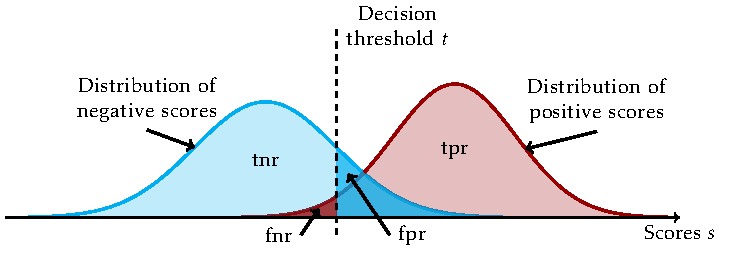
\includegraphics{images/confusion_rates.pdf}
  \caption{The relation between classification scores and  rates. The blue curve is the theoretical distribution of the scores of negative samples, and the red curve the theoretical distribution of the scores of positive samples. Filled areas with light blue or light red represent true-negative and true-positive rates. Similarly, the filled areas with dark blue or dark red represent false-positive and false-negative rates.}
  \label{fig: scores and rates}
\end{figure}

The confusion matrix is not the only way to measure the performance of binary classifiers. For example, there are many different classification matrices, and many of them are derived directly from the confusion matrix~\cite{fawcett2006introduction, metz1978basic, brodersen2010balanced, hossin2015review}. As an example, we can mention accuracy and balanced accuracy defined by
\begin{align*}
  \accuracy & = \frac{\tp + \tn}{n} &
  \baccuracy & = \frac{\tpr + \tnr}{2}
\end{align*}
At the end of this chapter, we provide Table~\ref{tab: classification metrics} that summarizes all classification metrics used in this work. Moreover, in the following section, we introduce a different approach for the performance evaluation of binary classifiers.

\subsection{ROC Analysis}\label{subsec: ROC}

In the previous section, we defined a general binary classification formulation~\eqref{eq: Binary classification counts} that minimizes a weighted sum of false-positive and false-negative counts. Therefore, we always have to find some trade-off between the false-positive and false-negative counts and select the best hyperparameters~$\lambda_1,$ $\lambda_2,$ for given tasks. There is no universal truth, which of these two errors is worse. For example, It is probably better to classify a healthy patient as sick and do additional tests than the other way around. On the other hand, in computer security, an antivirus program with a lot of false-positive alerts is useless since it is disruptive to the user. One way to visualize the trade-off between false-positive and false-negative errors is Receiver Operating Characteristic (ROC) space~\cite{egan1975signal, fawcett2006introduction}.

ROC space is a two-dimensional space with the x-axis equal to the false-positive rate and the y-axis to the true-positive rate. The left-hand side of Figure~\ref{fig: roc space} shows the ROC space with five highlighted points. Each point in the ROC space represents one fixed classifier, i.e., one pair of model~$f$ and decision threshold~$t.$ There are several important points in the ROC space. The point~$(0, 0)$ represents a classifier classifying all samples as negative, while~$(1, 1)$ is a classifier classifying all samples as positive. Both these classifiers are useless. On the other hand, the point~$(0, 1)$ represents the perfect classifier. Generally, we can say that one classifier is better than another if its representation in ROC space is to the northwest of the second one. In such a case, the classifier has a higher true-positive rate and lower false-positive rate than the second one. For example, in Figure~\ref{fig: roc space}, classifier \textbf{B} is better than classifier \textbf{C}. On the other hand, it is impossible to say which classifier is better if one has a higher true-positive rate and the other has a lower false-positive rate. We can see this situation for classifier \textbf{B} and \textbf{A}. In such a case, the preference depends on the given problem, as discussed at the beginning of this section.

Another important part of the ROC space is the diagonal line highlighted in red in Figure~\ref{fig: roc space}. Any classifier that appears on this diagonal provides the same performance as a random classifier. For example, classifier \textbf{C} is represented in ROC space by point~$(0.7, 0.7).$ It means that this classifier randomly classifies 70\% of samples as positive. Therefore, any classifier that appears in ROC space in the lower right triangle is worse than a random classifier. There are usually no classifiers in this area since any classifier from the lower right triangle can be easily improved. If we negate the decision of such a classifier for every sample, we get its negated version in the upper left triangle. Such a situation is in Figure~\ref{fig: roc space} for classifier \textbf{E} and \textbf{B}. We negate every decision of classifier \textbf{E}. Therefore,  all true-positive samples became false-negative and vice versa. Since classifier \textbf{E} has a false-negative rate of 0.8, we can deduce that negated classifier will have a true-positive rate of 0.8. Similarly, since classifier \textbf{E} has a true-negative rate of 0.4, its negated version will have a false-positive rate of 0.4. Therefore the negated version of classifier \textbf{E} is represented in ROC space by point~$(0.4, 0.8),$ which is classifier~\textbf{B}.

\begin{figure}
  \centering
  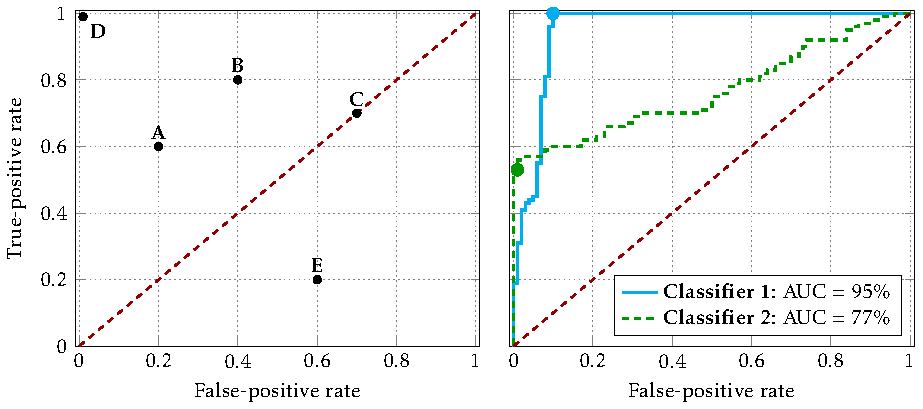
\includegraphics{images/roc_space.pdf}
  \caption{A basic representation of the ROC space with five different classifiers. (\textbf{left}) A comparison of ROC curves for two different classifiers. (\textbf{right})}
  \label{fig: roc space}
\end{figure}

Many classifiers produce directly a decision that samples are positive or negative. As an example, we can mention decision trees. Such classifiers are always represented as a single point in the ROC space. Moreover, this class of classifiers does not fit into our description from Notation~\ref{not: classifier} since such classifiers do not provide any classification scores. In this text, we restrict to the classifiers as defined in Notation~\ref{not: classifier}. We assume that the classifier consists of the model~$f$ that produces classification scores and the decision threshold~$t.$ Many standard classifiers such as neural networks or logistic regression fall into this setting. Even though the decision threshold is determined during the training process, it is possible to change it and obtain different predictions. This possibility is very often used to produce so-called ROC curves~\cite{fawcett2006introduction}. ROC curve represents how model~$f$ behaves for different thresholds~$t$ varying from~$-\infty$ to~$+\infty.$ Right-hand side of Figure~\ref{fig: roc space} provides an example of two ROC curves for two different classifiers. \textbf{Classifier 1} provides accuracy~95\% and is represented by the blue dot, while the blue line represents its ROC curve. \textbf{Classifier 2} represented by the green dot provides accuracy~76\%, and the green dashed line represents its ROC curve. A standard method how for comparing two classifiers using ROC curves is to compare corresponding areas under the ROC curves (AUC)~\cite{bradley1997use, hanley1982meaning}. Such an approach is a simple way to reduce the ROC curve to one number. In the case of standard binary classification, the larger the AUC, the better. In Figure~\ref{fig: roc space} we can see that the blue classifier has AUC 95\% while the green one has only 77\%. Therefore, for most classification problems, the blue classifier is better.

Since both false-positive and true-positive rates are non-increasing functions of threshold~$t,$ we can efficiently compute the ROC curve from sorted classification scores~$\bm{s}$ given by the model~$f.$ In Algorithm~\ref{alg: roc curve} we show an efficient algorithm for generating the ROC curve. This algorithm gives us an interesting insight into ROC curves: ROC curves represent the ability of the model to rank the positive samples higher than the negative ones~\cite{fawcett2006introduction}. Moreover, the AUC of a classifier is equivalent to the probability that the classifier will rank a randomly chosen positive sample higher than a randomly chosen negative sample~\cite{fawcett2006introduction}. By comparing the classifiers from the right-hand side of Figure~\ref{fig: roc space}, we can deduce that \textbf{Classifier 1} is generally better at a false-positive rate larger than~$0.01.$ Otherwise, \textbf{Classifier 2} is the better one. Therefore,  there is a specific region of the ROC space where \textbf{Classifier 2} outperforms \textbf{Classifier 1}. In the next section, we discuss multiple different problems which focus on the performance only at low false-positive rates.

\begin{algorithm}
  \centering
  \begin{algorithmic}[1]
    \Require Sorted classification scores~$\bm{s}_{[\cdot]}$ in decreasing order~$s_{[1]} \geq \dots \geq s_{[n]}$
    \State Set $\tp \gets 0,$ $\fp \gets 0,$ $s_{\text{prev}} = +\infty,$ and an empty set~$ROC = \{~\}$ of points in ROC space
    \For{$l \in \{1, \ldots, \nall\}$}
      \If{$s_{[i]} \neq s_{\text{prev}}$} 
        \State push~$(\nicefrac{\fp}{\nneg}, \nicefrac{\tp}{\npos})$ into~$ROC$
      \EndIf
      \If{$y_{[i]} = 1$}
        \State $\tp \gets \tp + 1$
      \Else
        \State $\fp \gets \fp + 1$
      \EndIf
    \EndFor
    \State push~$(\nicefrac{\fp}{\nneg}, \nicefrac{\tp}{\npos}) = (1, 1)$ into~$ROC$
  \end{algorithmic}
  \caption{Efficient algorithm~\cite{fawcett2006introduction} for generating ROC curve from sorted classification scores.}
  \label{alg: roc curve}
\end{algorithm}

\section{Classification at the Top}\label{sec: related problems}

As we discussed in the previous sections, standard binary classification aims to separate positive and negative samples with the lowest possible error on the whole dataset. The performance of a binary classifier can be measured using classification metrics such as accuracy or using ROC curves and their AUC. However, it is desirable to focus only on a small number of the most relevant samples in many applications. In such a case, the goal is to maximize the performance only on the relevant samples. Since the rest of the samples are irrelevant, their performance is unimportant. Figure~\ref{fig: standard vs. aatp} shows the difference between the standard classifier (\textbf{Classifier 1}) that maximizes the accuracy and the classifier that focuses only on the classification at the top (\textbf{Classifier 2}). In this particular case, \textbf{Classifier 2} maximizes the number of positive samples that are ranked higher than the worst negative sample. Formally, \textbf{Classifier 2} maximizes the following metric
\begin{equation}\label{eq: metric pos at top}
  \postop(\bm{s}) = \frac{1}{\npos} \sum_{i \in \Ipos} \Iverson{s_i \geq \max_{j \in \Ineg}s_j}.
\end{equation}
For both classifiers, Figure~\ref{fig: standard vs. aatp} shows two different decision thresholds. The black threshold is the one for which the classifier was trained, while the green one represents the worst negative sample. For \textbf{Classifier 2} these two thresholds coincide. We can observe that \textbf{Classifier 1} provides a much better separation of positive and negative samples. Only a few samples above the black threshold ruin perfect separation. On the other hand, the separation provided by \textbf{Classifier 2} is much worse since half of the positive samples are mixed with negative ones. Therefore, the accuracy of \textbf{Classifier 1} is~$95\%$ while the accuracy of \textbf{Classifier 2} is only~$76\%.$ However, in terms of metric~\eqref{eq: metric pos at top} the situation is quite different. Since there are few negative outliers, there is only 19\% of positive samples above the worst negative for \textbf{Classifier 1}. \textbf{Classifier 2} achieves to push 53\% of positive samples above the worst negative and therefore provides better performance for this case. The same behavior can also be demonstrated using ROC curves as shown in Figure~\ref{fig: roc space log}. The blue line represents ROC curve for \textbf{Classifier 1} and the green dashed one for \textbf{Classifier 2}. There are two important points for \textbf{Classifier 1} in the figure. The first one is highlighted by an blue circle and represents the point in the ROC space that corresponds to the actual threshold. In other words, it corresponds to the black threshold from Figure~\ref{fig: standard vs. aatp}. The second point is highlighted by an blue square and corresponds to the green threshold from Figure~\ref{fig: standard vs. aatp}. Since for \textbf{Classifier 2} both thresholds coincide, there is only one point in Figure~\ref{fig: roc space log} highlighted by a green square. The superiority of \textbf{Classifier 1} in the overall performance is evident from the left-hand side of the figure. The AUC for \textbf{Classifier 1} is 95\% and only 77\% for \textbf{Classifier 2}. Moreover, we can see that there is only a small region of ROC space, where \textbf{Classifier 2} provides a higher true-positive rate. However, this region is very interesting. The right-hand side of Figure~\ref{fig: roc space log} provides the same ROC curves but with a logarithmic x-axis. The logarithmic scale allows us to concentrate on very low false-positive rates. We can see, that if the false-positive rate is lower than~$7 \cdot 10^{-1},$ then \textbf{Classifier 2} provides better true-positive rate than \textbf{Classifier 1}. It means that in this region of the ROC space, \textbf{Classifier 2} provides better sorting of positive and negative samples, i.e., more positive samples are ranked higher than negative ones. Moreover, classification metric~\eqref{eq: metric pos at top} is equivalent to the y-coordinate at the lowest non-zero false-positive rate. It is evident from the right-hand side of Figure~\ref{fig: roc space log} where the value of metric~\eqref{eq: metric pos at top} is highlighted using squares for both classifiers.

\begin{figure}
  \centering
  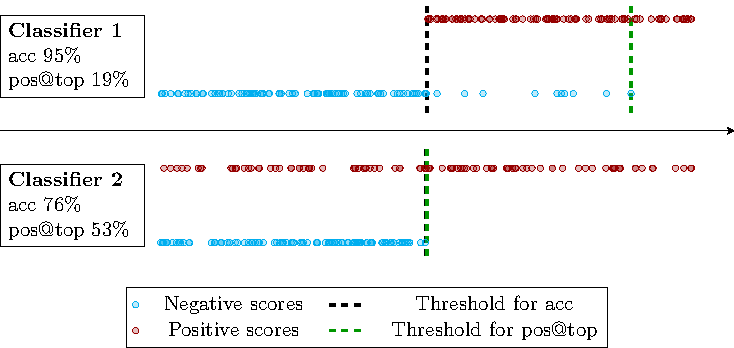
\includegraphics{images/standard_aatp_comparison.pdf}
  \caption{Difference between standard classifiers (\textbf{Classifier~1}) and classifiers maximizing~$\postop$ metric (\textbf{Classifier~2}). While the former has a good total~$\accuracy$, the latter has a good~$\postop$ metric.}
  \label{fig: standard vs. aatp}
\end{figure}

\begin{figure}
  \centering
  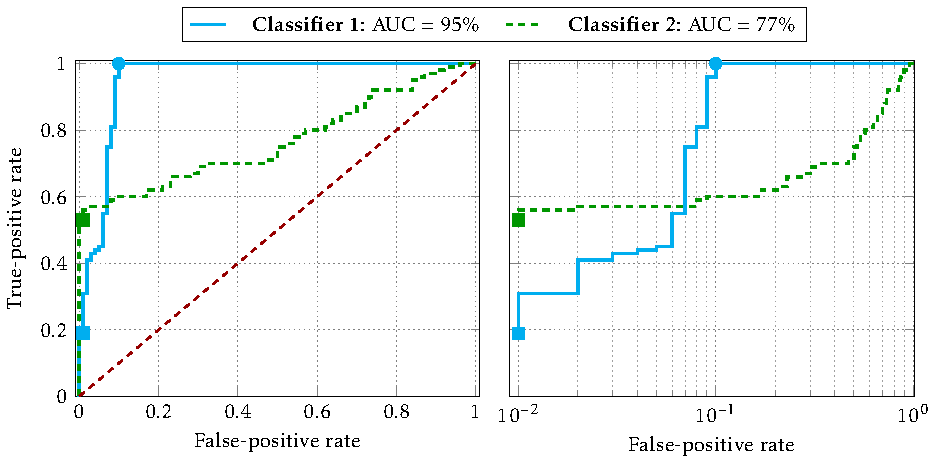
\includegraphics{images/roc_space_log.pdf}
  \caption{Difference between standard classifiers (\textbf{Classifier~1}) and classifiers maximizing~$\postop$ metric (\textbf{Classifier~2}). While the former has a good total~$\accuracy$, the latter has a good~$\postop$ metric.}
  \label{fig: roc space log}
\end{figure}

As discussed above, \textbf{Classifier 1} focuses on the overall performance, while the  \textbf{Classifier 2} on the performance on low false-positive rates. The latter classifier can be handy for search engines such as Google or DuckDuckGo, where the goal is to have all relevant results on the first few pages. The results on page 50 are usually of no interest to anyone, so it is crucial to move the most relevant results to the few first pages~\cite{cortes2003auc}. Therefore, it is essential to push as many positive samples above some small portion of negative samples. The rest of the chapter presents three main categories of problems that solve this kind of problem. Moreover, in the next chapter, we show that at least some formulations from these three categories are closely related to binary classification.

\subsection{Ranking Problems}

The first category is ranking problems. The ranking algorithms play a crucial role in many information retrieval problems:
\begin{itemize}
  \item \textbf{Document (Text) retrieval systems} are used for obtaining relevant documents from the collection of documents based on the relevance to the user's query. Such systems are widely used for accessing books, journals, or any other documents. However, the most visible application is search engines such as Google or DuckDuckGo.
  \item \textbf{Collaborative filtering} is one of the techniques used to predict the user's rating of a new product based on the past ratings of users with similar rating patter. Such systems can be used to generate music or video playlist automatically. Therefore, such systems are widely used in services such as Youtube or Spotify.
\end{itemize}
The two examples above show that ranking problems usually depend on users' feedback or preferences. In binary classification, we have only the labels that represent if the samples are positive or negative. On the other hand, ranking problems use multiple ways to describe the users' feedback. One approach uses the feedback function~$\Phi: \R^d \times \R^d \to \R$ to represent the user's preferences~\cite{freund2003efficient}. In such a case, the feedback function can be defined for all pairs of samples~$(\bm{x}_i, \bm{x}_j)$ in the following way
\begin{equation*}
  \Phi(\bm{x}_i, \bm{x}_j) \; 
  \begin{cases}
    > 0 & \bm{x}_i \text{ is prefered over } \bm{x}_j, \\
    = 0 & \text{no preference,} \\
    < 0 & \bm{x}_j \text{ is prefered over } \bm{x}_i.
  \end{cases}
\end{equation*}
We can see, that the feedback function specify if the user prefers~$\bm{x}_i$ over~$\bm{x}_j$ or not. Moreover, the feedback function also specifies how strong the preference is, i.e., the higher the volume~$\abs{\Phi(\bm{x}_i, \bm{x}_j)}$ is the more important the preference is. Many ranking algorithms try to find some ordering of all samples that minimizes the number of wrongly ordered pairs of samples concerning the given feedback function. Consider ranking function~$r: \R^d \to \R.$ The sample~$\bm{x}_i$ is ranked higher than sample~$\bm{x}_j$ if~$r(\bm{x}_i) > r(\bm{x}_j).$ Then, the minimization of the number of misordered pairs can be formally written as follows
\begin{mini}{r}{
  \sum_{i \in \I} \sum_{j \in \I} \Iverson{r(\bm{x}_i) \leq r(\bm{x}_j)} \cdot \max\Brac[c]{0, \; \Phi(\bm{x}_i, \bm{x}_j)}.
  }{\label{eq: rankboost}}{}
\end{mini}
This problem is hard to solve since the objective function contains a pairwise comparison of all samples. Therefore, the problem is not suitable for large data. \emph{RankBoost}~\cite{freund2003efficient} is an boosting algorithm based on the AdaBoost~\cite{freund1997decision} that combines many weak ordering functions to obtain the final ranking. This approach leads to the maximization of the area under the ROC curve~\cite{rudin2009pnorm}. Therefore, RankBoost focuses on the overall performance. However, as we discussed at the beginning of the section, we want to focus only on the small portion of the most relevant samples in many applications. In such a case, this approach is not ideal.

Consider recommendation of movies. In such a case, we only care about if the movie is good or not. What is not important is if one bad movie is ranked higher than another bad movie. Both movies are still bad and therefore not relevant. Many ranking algorithms~\cite{rudin2009pnorm} use the so-called bipartite ranking to address this situation. In such a situation, each sample is positive (good) or negative (bad), and the goal is to push positive samples above negative ones. The authors of~\cite{rudin2009pnorm} proposed the following formulation
\begin{mini}{r}{
  \sum_{j \in \Ineg} \Brac{\sum_{i \in \Ipos} \Iverson{r(\bm{x}_i) \leq r(\bm{x}_j)}}^p.
  }{\label{eq: p-norm push}}{}
\end{mini}
The authors of~\cite{rudin2009pnorm} also proposed boosting algorithm called \textbf{$p$-Norm Push} to solve the formulation above. Note that for~$p = 1$, the formulation~\eqref{eq: p-norm push} is very similar to the RankBoost~\eqref{eq: rankboost}. In such a case, the resulting ranking function maximizes the AUC and therefore optimizing overall rankig. On the other hand, for~$p \rightarrow +\infty$, the formulation~\eqref{eq: p-norm push} minimizes the largest number of positive samples ranked below any negative sample
\begin{mini}{r}{
  \max_{j \in \Ineg} \; \sum_{i \in \Ipos} \Iverson{r(\bm{x}_i) \leq r(\bm{x}_j)}.
  }{\label{eq: p-norm push infty}}{}
\end{mini}
In such a case, the resulting ranking function focus only on the absolute top, i.e., it aims to push as many positive samples above the negative sample with the highest rank. Authors of~\cite{agarwal2011infinite} focus on formulation~\eqref{eq: p-norm push infty} with~$p \rightarrow + \infty$  and introduces SVM (\emph{Support Vector Machines}~\cite{cortes1995support}) based algorithm called \emph{Infinite Push} to solve it. The major problem of formulation~\eqref{eq: p-norm push infty} is that the objective still contains the pairwise comparison of positive and negative samples. Therefore the formulation is not suitable for large data. To mitigate this issue, the authors of~\cite{li2014top} proposed an equivalent formulation in the following form
\begin{mini}{r}{
  \sum_{i \in \Ipos} \Iverson{r(\bm{x}_i) \leq \max_{j \in \Ineg} \; r(\bm{x}_j)}.
  }{\label{eq: toppush rank}}{}
\end{mini}
Moreover, authors of~\cite{li2014top} proposed \TopPush algorithm with the linear complexity in the number of samples. Note that the objective function of the problem above is almost the same as the metric~\eqref{eq: metric pos at top}. Therefore, this \textbf{Classifier 2} from Figures~\ref{fig: standard vs. aatp} and~\ref{fig: roc space log} corresponds to the ranking function given by \TopPush algorithm. It shows a tied connection between binary classification and the bipartite ranking problems. 

\subsection{Accuracy at the Top}

In the previous section, we introduced formulation~\eqref{eq: toppush rank}, which focuses on maximizing the number of positive samples above the worst negative sample (the one with the highest rank or highest classification score). This formulation is very useful, as discussed at the beginning of this section. However, such a maximization problem can be unstable since the objective function does not allow false-positive errors. Therefore, if there is one negative outlier with a high score, the number of positive samples above this outlier can be tiny. The authors of~\cite{boyd2012accuracy} focus on similar problems as \TopPush, but use a different approach. They proposed a formulation called \textbf{Accuracy at the Top} which aims to maximize the number of positive samples in the top $\tau$-fraction of all samples. The top $\tau$-fraction of all samples can be formally defined as samples with scores higher then the top $\tau$-quantile of all scores
\begin{mini}{f}{
  \frac{1}{\nneg} \fp(\bm{s}, t) + \frac{1}{\npos} \fn(\bm{s}, t)
  }{\label{eq: aatp intro}}{}
  \addConstraint{s_i}{= f(\bm{x}_i), \quad i \in \I}
  \addConstraint{t}{= \max \Set{t}{\frac{1}{n} \sum_{i \in \I} \Iverson{s_i \geq t} \geq \tau},}
\end{mini}
where~$f: \R^d \to \R$ is a model. Even though the goal is to maximize the number of positive samples above the top $\tau$-quantile, the objective function contains false-positive and false-negative rates. It should be sufficient to include only one of them since the definition of the threshold implies the minimization of the other one as well. However, this form of objective function should be more robust~\cite{grill2016learning}. The problem of Accuracy at the Top is useful, for example, in applications where identified samples undergo expensive post-processing, such as human evaluation. For example, potentially useful drugs need to be preselected and manually investigated in drug development. Since the manual investigation is costly, we have to select only a fraction of drugs with the highest potential. However, it is precisely what Accuracy at the Top does.

There are many methods on how to solve Accuracy at the Top. The early approaches aim at solving approximations. For example, the authors of \cite{joachims2005svm} optimize a convex upper bound on the number of errors among the top samples. Due to exponentially many constraints, the method is computationally expensive. In \cite{boyd2012accuracy} the authors presented an SVM-like formulation. They assume that the top $\tau$-quantile is one of the samples, construct~$n$ unconstrained optimization problems with fixed thresholds, solve them and select the best solution. While this removes the necessity to handle the (difficult) quantile constraint, the algorithm is computationally infeasible for a large number of samples. The authors of~\cite{grill2016learning} proposed the projected gradient descent method, where after each gradient step, the quantile is recomputed. In \cite{eban2017scalable} authors suggested new formulations for various criteria and argued that they keep desired properties such as convexity. Finally, the authors of~\cite{tasche2018plug} showed that Accuracy at the Top is maximized by thresholding the posterior probability of the relevant class.

\subsection{Hypothesis Testing}

The hypothesis testing operates with null~$H_0$ and alternative~$H_1$ hypothesis. The goal is to either reject the null hypothesis in favor of the alternative or not. Since this problem is binary, two possible errors can occur. Type I occurs when~$H_0$ is true but is rejected, and Type II error happens when~$H_0$ is false but fails to be rejected. The Neyman-Pearson problem minimizes~\cite{neyman1933ontheproblem} Type II error while keeping Type I error smaller than some predefined bound. Using our notation for the Neyman-Pearson problem, the null hypothesis~$H_0$ states that sample~$\bm{x}$ has a negative label. Then Type I error occurs when the sample is false-positive, while Type II error occurs when the sample is false-negative. Therefore, the Neyman-Pearson problem minimizes the false-negative rate with the prescribed level~$\tau$ of the false-positive rate. Such constraint can be written in the form of quantile, i.e., the threshold is the top $\tau$-quantile of scores of all negative samples.
\begin{mini*}{f}{
  \frac{1}{\npos} \fn(\bm{s}, t)
  }{}{}
  \addConstraint{s_i}{= f(\bm{x}_i), \quad i \in \I}
  \addConstraint{t}{= \max \Set{t}{\frac{1}{\nneg} \sum_{i \in \Ineg} \Iverson{s_i \geq t} \geq \tau},}
\end{mini*}
This formulation is very similar to the one for Accuracy at the Top~\eqref{eq: aatp intro}. The main difference is that the quantile in the constraint is not computed from all but only from negative samples. Also, note one key difference in interpretation. The~$\tau$ in Accuracy at the Top represents the total amount of samples we want to process with the smallest possible error. On the other hand, in the Neyman-Pearson problem~$\tau$ represents the maximal acceptable false-positive rate. Therefore, the former approach is useful in situations where we can process only a certain number of samples. The latter is for situations where we have strict constraints on false-positive errors.

\pagebreak

\section{Summary}

In this chapter, we introduced the general formulation~\eqref{eq: Binary classification counts} for binary classification and discussed how to measure the performance of binary classifiers. The first approach for performance evaluation is based on the confusion matrix. This approach is very straightforward. Moreover, it is possible to derive many different classification matrices from the confusion matrix. Table~\ref{tab: classification metrics} summarizes classification matrices derived from the confusion matrix used in the upcoming chapters. The second approach introduced in this chapter uses the ROC space to visualize the ability of classifiers to rank positive samples above negative ones. Since standard binary classification focuses on optimizing the overall performance, we discussed that there are many problems closely tied to the binary classification that focuses on the performance only of the most relevant samples. Such problems occur in many applications, from search engines to drug development. We also introduced Ranking problems, the problem of Accuracy at the Top, and the Neyman-Pearson problem and discussed their relation to the binary classification. In the upcoming chapters, we focus on these three groups of problems and introduce a general framework to handle them.

\begin{table}
  \centering
  \begin{NiceTabular}{ccc}
    \CodeBefore
      \rowcolor{\headercol}{1}
      \rowcolors{3}{\rowcol}{}[restart]
    \Body
    \toprule
    \textbf{Name} & \textbf{Aliases} & \textbf{Formula} \\
    \midrule
    true negatives
      & correct rejection
      & $\tn$ \\
    false positives
      & Type I error, false alarm
      & $\fp = \nneg - \tn$ \\
    true positives
      & hit
      & $\tp$ \\
    false negatives
      & Type II error
      & $\fn = \npos - \tp$ \\
    \midrule
    true negative rate
      & specificity, selectivity
      & $\tnr = \frac{\tn}{\nneg}$ \\
    false positive rate
      & fall-out
      & $\fpr = \frac{\fp}{\nneg} = 1 - \tnr$ \\
    true positive rate
      & sensitivity, recall, hit rate
      & $\tpr = \frac{\tp}{\npos}$ \\
    false negative rate
      & miss rate
      & $\fnr = \frac{\fn}{\npos} = 1 - \tpr$ \\
    \midrule
    accuracy
      & ---
      & $\accuracy = \frac{\tp + \tn}{n}$ \\
    balanced accuracy
      & ---
      & $\baccuracy = \frac{\tpr + \tnr}{2}$ \\
    precision
      & positive predictive value
      & $\precision = \frac{\tp}{\tp + \fp}$ \\
    \bottomrule
  \end{NiceTabular}
  \caption{Summary of classification metrics derived from confusion matrix. The first column shows the name used in this work, while the second column shows alternative names that can be found in the literature. The last column shows the formula based on the confusion matrix.}
  \label{tab: classification metrics}
\end{table}
\chapter{Introduction to Binary Classification}

The problem of data classification is very important in the modern world. The classification aims to find a relation between a set of objects and target variables based on some objects' properties. The properties of the objects are usually called features, and the target variables are usually called labels. Many real-world problems can be formulated as classification tasks:
\begin{itemize}
  \item \textbf{Medical Diagnosis:} In medicine, the classification is often used to improve disease diagnosis. In such a case, the features are medical records such as the patient's blood tests, temperature, or roentgen images. The target variable is if the patient has some disease. For example, classification can be used to process mammogram images and detect cancer~\cite{viale2012current, levy2016breast}.
  \item \textbf{Internet Security:} These days, the internet is a crucial part of our lives. With the increasing usage of the internet, the number of attacks increases as well. An essential part of the defense is intrusion detection systems~\cite{grill2016learning, scarfone2007guide} that search for malicious activities (network attacks) in network traffic. Classification can be used to improve such systems as shown in~\cite{giacinto2002intrusion, shanbhag2009accurate}.
  \item \textbf{Marketing:} In marketing, the task can be to classify customers based on their buying interests. Such information can be used to build a personalized recommendation system for customers and therefore increase income~\cite{kaefer2005neural, zhang2007building}.
\end{itemize}
Besides these three examples, applications of classification can be found in almost every academic or even industrial field. Furthermore, a vast number of algorithms try to solve classifications problems. Typically these algorithms consist of three phases:
\begin{itemize}
  \item \textbf{Training:} The classification problems usually fall into the category of supervised learning. It means that we assume the prior knowledge of the target classes in the training phase. The training data typically consists of pairs (sample, label) and can be described as follows
  \begin{equation*}\label{eq: training set}
    \mathcal{D}_{\mathrm{train}} = \Brac[c]{(\bm{x}_i, y_i)}_{i=1}^{n},
  \end{equation*}
  where the sample~$\bm{x}_i \in \R^d$ is a~$d$-dimensional vector of features that describes the object of interes and the label~$y_i \in \{1, 2, \ldots, k\}$ represents target class. Moreover~$n \in \N$ is a number of training samples and~$k \in \N$ is a number of target classes. In this phase, the algorithm uses the training data to learn a model, i.e., set model parameters according to some predefined criterion, to describe the training data as best as possible.
  \item \textbf{Validation:} All algorithms usually have some hyperparameters that can be changed to improve the resulting model. The validation phase is used to select the best hyperparameter settings that lead to the most performant and robust model.
  \item \textbf{Testing:} In the testing phase, the model is used to assign labels~$\hat{y}_i \in \{1, 2, \ldots, k\}$ to the data from the testing set, which is not known during the training phase.
\end{itemize}
The previous definition of the training set is general for any classification problem with multiple classes. However, we focus on the special subclass of classification problems called binary classification in this work. The binary classification is a special case of classification in which the number of classes is~$k=2.$ These two classes are usually referred to as negative and positive classes. Moreover, the positive class is usually the one we are more interested. Returning to example with cancer, the positive class would represent that the patient has cancer while the negative that the patient is healthy.

\begin{notation}[Dataset]\label{not: dataset}
  In this work, we use label~$0$ to encode the negative class and label~$1$ to encode the positive class. Moreover, by a dataset of size~$n \in \N$ we mean a set of pairs in the following form
  \begin{equation*}
    \mathcal{D} = \Brac[c]{(\bm{x}_i, y_i)}_{i=1}^{n},
  \end{equation*}
  where~$\bm{x}_i \in \R^d$ represents samples,~$d \in \N$ its dimension and~$y_i \in \{0, 1\}$ corresponding labels. To simplify future notation, we denote a set of all indices of dataset~$\mathcal{D}$ as~$\I = \Ineg \cup \Ipos,$ where
  \begin{equation*}
    \begin{aligned}
      \Ineg & = \Set{i}{i \in \{1, 2, \ldots, n\} \; \land \; y_i = 0}, \\
      \Ipos & = \Set{i}{i \in \{1, 2, \ldots, n\} \; \land \; y_i = 1}.
    \end{aligned}
  \end{equation*}
  We also denote the number of negative samples in~$\mathcal{D}$ as~$\nneg = \Brac[v]{\Ineg}$ and the number of positive samples in~$\mathcal{D}$ as~$\npos = \Brac[v]{\Ipos},$ i.e. total number of samples is~$n = \nneg + \npos.$ 
\end{notation}

The goal of any classification problem is to classify given samples with the highest possible accuracy or, in other words, with the lowest possible error. In the case of binary classification, there are two types of error: positive sample is classified as negative and vice versa. Formally, using the Notation~\ref{not: dataset}, the minimization of these two types of errors can be written as follows
\begin{mini}{\bm{w}, t}{
    C_1 \sum_{i \in \Ineg} \Iverson{s_i \geq t} + C_2 \sum_{i \in \Ipos} \Iverson{s_i < t}
  }{\label{eq: Binary classification}}{}
  \addConstraint{s_i}{= f(\bm{x}_i; \bm{w}), \quad}{i \in \I,}
\end{mini}
where~$C_1, C_2 \in \R,$ the function~$f \colon \R^d \to \R$ is called model and~$\Iverson{\cdot{}}$ is Iverson function that is used to counts misclassified samples and is defined as
\begin{equation}\label{eq: iverson}
  \Iverson{x} = \begin{cases}
    0 & \quad \text{if } x \text{ is false}, \\
    1 & \quad \text{if } x \text{ is true}.
  \end{cases}
\end{equation}
Moreover, the vector~$\bm{w} \in \R^d$ represents trainable parameters (weights) of the model~$f$ and~$t \in R$ represents a decision threshold. The parameters~$\bm{w}$ are determined from training data during the training phase of the algorithm. Although the decision threshold~$t$ can also be determined from the training data, in many cases, it is fixed. For example, many algorithms assume that the classification score~$s_i = f(\bm{x}_i; \bm{w})$ given by the model~$f$ represents the probability that the sample~$\bm{x}_i$ belongs to the positive class. Therefore, the decision threshold is set to~$t = 0.5,$ and the sample is classified as positive if its classification score is larger than this threshold. In Notation~\ref{not: classifier}, we summarize the notation that is used in the rest of the work.

\pagebreak

\begin{notation}[Classifier]\label{not: classifier}
  By classifier, we always mean pair of model~$f$ and corresponding decision threshold~$t$. By model, we mean a function $f \colon \R^d \to \R$ which maps samples~$\bm{x}$ to its classification scores~$s$, i.e. for all~$i \in \I$ the classification score is defined as
  \begin{equation*}
    s_i = f(\bm{x}_i; \; \bm{w}),
  \end{equation*}
  where~$\bm{w}$ represents trainable parameters (weights) of the model. Predictions are defined for all~$i \in \I$ in the following way
  \begin{equation}\label{eq: prediction}
    \hat{y}_i = \begin{cases}
      1 & \quad \text{if } s_i \geq t, \\
      0 & \quad \text{otherwise.}
    \end{cases}
  \end{equation}
\end{notation}

\section{Performance Evaluation}\label{sec: performance evaluation}

In the previous section, we defined general binary classification problem~\eqref{eq: Binary classification}. However, we did not discuss how to measure the performance of the resulting classifier. In this section, we introduce basic performance metrics  that are used to measure the performance of binary classifiers.

\subsection{Confusion Matrix}

Based on the prediction~$\hat{y}_i$ from~\eqref{eq: prediction} and an actual label~$y_i$ of the sample~$\bm{x}_i,$ each sample can be assigned to one of the four following categories:
\begin{itemize}
  \item \textbf{True negative:} sample~$\bm{x}_i$ is negative and is classified as negative, i.e.~$y_i = 0 \; \land \; \hat{y}_i = 0.$
  \item \textbf{False positive:} sample~$\bm{x}_i$ is negative and is classified as positive, i.e.~$y_i = 0 \; \land \; \hat{y}_i = 1.$
  \item \textbf{False negative:} sample~$\bm{x}_i$ is positive and is classified as negative, i.e.~$y_i = 1 \; \land \; \hat{y}_i = 0.$
  \item \textbf{True positive:} sample~$\bm{x}_i$ is positive and is classified as positive, i.e.~$y_i = 1 \; \land \; \hat{y}_i = 1.$
\end{itemize}
If we assign each sample from dataset~$\mathcal{D}$ to one of the categories above and count the number of samples in each of these four categories, we get the confusion matrix (sometimes also called contingency table)~\cite{fawcett2006introduction}, see Figure~\ref{fig: confusion matrix}. A confusion matrix consists of four fields that contains number of true-negative (\textbf{tn}), false-positive (\textbf{fp}), false-negative (\textbf{fn}), and true-positive (\textbf{tp}) samples in the whole dataset. More formally, using the prediction rule~\eqref{eq: prediction} we can compute all fields of the confusion matrix as follows
\begin{equation}\label{eq: confusion counts}
  \begin{aligned}
    \tp(\bm{s}, t) & = \sum_{i \in \Ipos}\Iverson{s_i \geq t}, & \quad
    \fn(\bm{s}, t) & = \sum_{i \in \Ipos}\Iverson{s_i < t}, \\
    \tn(\bm{s}, t) & = \sum_{i \in \Ineg}\Iverson{s_i < t}, & \quad
    \fp(\bm{s}, t) & = \sum_{i \in \Ineg}\Iverson{s_i \geq t},
  \end{aligned}
\end{equation}
where~$\bm{s}$ is the vector of classification scores given by model~$f,$ and~$\Iverson{\cdot}$ is the Iverson function~\eqref{eq: iverson}. In the following text, we sometimes use simplified notation~$\tp = \tp(\bm{s}, t)$ (and similar notation for other counts). In such cases, the vector of classification scores and decision threshold is fixed and is known from the context. Using the simplified notation, we can define true-positive, false-positive, true-negative, and false-negative rates as follows
\begin{equation}\label{eq: confusion rates}
  \begin{aligned}
    \tpr & = \frac{\tp}{\npos}, & \quad
    \fnr & = \frac{\fn}{\npos}, & \quad
    \tnr & = \frac{\tn}{\nneg}, & \quad
    \fpr & = \frac{\fp}{\nneg}.
  \end{aligned}
\end{equation}
Figure~\ref{fig: scores and rates} shows the relation between classification rates and the decision threshold. The blue and red curves represent the theoretical distribution of the scores of negative and positive samples, respectively. If we increase the value of the threshold~$t,$ we decrease the false-positive rate, but at the same time, we also increase the false-negative rate. On the other hand, if we decrease the value of~$t,$ we decrease the false-negative rate, but at the same time, we also increase the false-positive rate. In other words, it is not possible to decrease the false-positive rate only by moving the threshold~$t$ without increasing the false-negative rate and vice versa. Therefore, we always have to find some balance between these two types of errors.

If we look at the general definition of the binary classification problem~\eqref{eq: Binary classification}, the objective function is just the weighted sum of false-positive and false-negative samples. Therefore, we can use the notation~\eqref{eq: confusion rates} and rewrite the problem~\eqref{eq: Binary classification} to
\begin{mini}{\bm{w}, t}{
    C_1 \cdot \fp(\bm{s}, t) + C_2 \cdot \fn(\bm{s}, t)
  }{\label{eq: Binary classification counts}}{}
  \addConstraint{s_i}{= f(\bm{x}_i; \bm{w}), \quad}{i \in \I.}
\end{mini}
The parameters~$C_1, \; C_2 \in \R$ are used to specify which error is more serious for the particular classification task.

\begin{figure}
  \centering
  \begin{NiceTabular}{cccccc}[cell-space-limits = 7pt]
    && \Block[draw=black, line-width=2pt, rounded-corners]{1-2}{
      \textbf{Predicted label}
    } \\
    && $\hat{y} = 0$
    &  $\hat{y} = 1$
    && \Block{1-1}{\textbf{Row total:}} \\
    \Block[draw=black, line-width=2pt, rounded-corners]{2-1}{
      \rotate \textbf{Actual} \\ \textbf{label}
    }
    & $y = 0$
    & \Block[draw=mygreen, fill=mygreen!50, rounded-corners]{1-1}{
      true \\ negatives \\ (\textbf{tn})
    }
    & \Block[draw=myred, fill=myred!50, rounded-corners]{1-1}{
      false \\ positives \\ (\textbf{fp})
    }
    & $\rightarrow$
    & \Block[draw=black, rounded-corners]{1-1}{all \\ negatives \\ ($\nneg$)} \\
    & $y = 1$
    & \Block[draw=myred, fill=myred!50, rounded-corners]{1-1}{
      false \\ negatives \\ (\textbf{fn})
    }
    & \Block[draw=mygreen, fill=mygreen!50, rounded-corners]{1-1}{
      true \\ positives \\ (\textbf{tp})
    }
    & $\rightarrow$
    & \Block[draw=black, rounded-corners]{1-1}{all \\ positives \\ ($\npos$)} \\
    && $\downarrow$
    &  $\downarrow$ \\
    \Block{1-2}{\textbf{Column} \\ \textbf{total:}}
    && \Block[draw=black, rounded-corners]{1-1}{all predicted \\ negatives}
    & \Block[draw=black, rounded-corners]{1-1}{all predicted \\ positives}
  \end{NiceTabular}
  \caption{The confusion matrix for the binary classification problem, where the negative class has label~$0$ and the positive class has label~$1.$ The true (target) label is denoted by~$y$ and predicted label is denoted by~$\hat{y}.$}
  \label{fig: confusion matrix}
\end{figure}

\begin{figure}
  \centering
  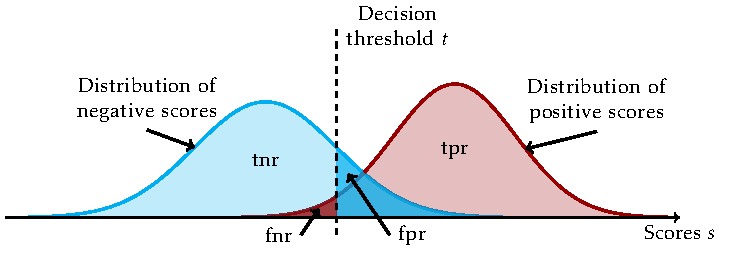
\includegraphics{images/confusion_rates.pdf}
  \caption{The relation between classification scores and  rates. The blue/red curve is the theoretical distribution of the scores of negative/positive samples, respectively. The area between the blue line and the x-axis is divided by the decision threshold~$t.$ The left part represents a true-negative rate, while the right part represents a false-positive rate. The area between the red line and the x-axis is also divided by~$t.$ The left part represents a false-negative rate, and a right represents the true-positive rate.}
  \label{fig: scores and rates}
\end{figure}

The confusion matrix is not the only way to measure the performance of binary classifiers. For example, there are many different classification matrices, and many of them are derived directly from the confusion matrix~\cite{fawcett2006introduction, metz1978basic, brodersen2010balanced, hossin2015review}. As an example, we can mention accuracy and balanced accuracy defined by
\begin{align*}
  \accuracy & = \frac{1}{n}\Brac{\tp + \tn} &
  \baccuracy & = \frac{1}{2}\Brac{\tpr + \tnr}
\end{align*}
Note that the objective function in~\eqref{eq: Binary classification counts} is accuracy if~$C_1 = C_2 = \frac{1}{\nall}.$ Moreover, for~$C_1 = \frac{1}{2\nneg}$ and~$C_2 = \frac{1}{2\npos},$ the objective function is balanced accuracy. This show the importance of these two performance matrices for standard binary classification. More performance metrics derived from the confusion matrix can be found in Table~\ref{tab: classification metrics}. Moreover, in the following section, we introduce a different approach for the performance evaluation of binary classifiers.

\begin{table}
  \centering
  \begin{NiceTabular}{ccc}
    \CodeBefore
      \rowcolor{\headercol}{1}
      \rowcolors{3}{\rowcol}{}[restart]
    \Body
    \toprule
    \textbf{Name} & \textbf{Aliases} & \textbf{Formula} \\
    \midrule
    true negatives
      & correct rejection
      & $\tn$ \\
    false positives
      & Type I error, false alarm
      & $\fp = \nneg - \tn$ \\
    true positives
      & hit
      & $\tp$ \\
    false negatives
      & Type II error
      & $\fn = \npos - \tp$ \\
    \midrule
    true negative rate
      & specificity, selectivity
      & $\tnr = \frac{\tn}{\nneg}$ \\
    false positive rate
      & fall-out
      & $\fpr = \frac{\fp}{\nneg} = 1 - \tnr$ \\
    true positive rate
      & sensitivity, recall, hit rate
      & $\tpr = \frac{\tp}{\npos}$ \\
    false negative rate
      & miss rate
      & $\fnr = \frac{\fn}{\npos} = 1 - \tpr$ \\
    \midrule
    accuracy
      & ---
      & $\accuracy = \frac{\tp + \tn}{n}$ \\
    balanced accuracy
      & ---
      & $\baccuracy = \frac{\tpr + \tnr}{2}$ \\
    precision
      & positive predictive value
      & $\precision = \frac{\tp}{\tp + \fp}$ \\
    \bottomrule
  \end{NiceTabular}
  \caption{Summary of classification metrics derived from confusion matrix. The first column shows the name used in this work, while the second column shows alternative names that can be found in the literature. The last column shows the formula based on the confusion matrix.}
  \label{tab: classification metrics}
\end{table}

\begin{figure}
  \centering
  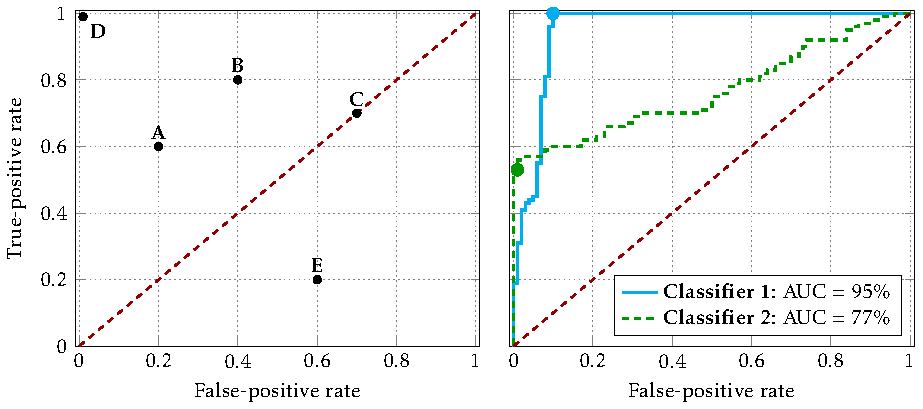
\includegraphics{images/roc_space.pdf}
  \caption{A basic representation of the ROC space with five different classifiers. (\textbf{left}) A comparison of ROC curves for two different classifiers. (\textbf{right})}
  \label{fig: roc space}
\end{figure}

\subsection{ROC Analysis}\label{subsec: ROC}

In the previous section, we defined a general binary classification formulation~\eqref{eq: Binary classification counts} that minimizes a weighted sum of false-positive and false-negative counts. Therefore, we always have to find some trade-off between the false-positive and false-negative counts and select the best hyperparameters~$C_1,$ $C_2,$ for given tasks. There is no universal truth which of these two errors is worse. For example, it is probably better to classify a healthy patient as sick and do additional tests than the other way around. On the other hand, in computer security, an antivirus program with a lot of false-positive alerts is useless since it is disruptive to the user. The Receiver Operating Characteristic (ROC) space~\cite{egan1975signal, fawcett2006introduction} is one way to visualize the trade-off between false-positive and false-negative errors.

ROC space is a two-dimensional space with the x-axis equal to the false-positive rate and the y-axis to the true-positive rate. The left-hand side of Figure~\ref{fig: roc space} shows the ROC space with five highlighted points. Each point in the ROC space represents one fixed classifier, i.e., one pair of model~$f$ and decision threshold~$t.$ There are several important points in the ROC space. The point~$(0, 0)$ represents a classifier classifying all samples as negative, while~$(1, 1)$ is a classifier classifying all samples as positive. Both these classifiers are useless. On the other hand, the point (0, 1) represents the perfect classifier that classifies all samples correctly since~$\fpr = 0$ and~$\tpr = 1.$

ROC representation allows us to decide whether one classifier is better than another, only in some cases. For example, in Figure~\ref{fig: roc space}, classifier \textbf{B} is better than classifier \textbf{C} since \textbf{B} has a higher true-positive rate and at the same time a lower false-positive rate. On the other hand, it is impossible to say which classifier is better if one has a higher true-positive rate and the other has a lower false-positive rate. We can see this situation for classifier \textbf{B} and \textbf{A}. In such a case, the preference depends on the given problem, as discussed at the beginning of this section.

Another important part of the ROC space is the diagonal line highlighted in red in Figure~\ref{fig: roc space}. Any classifier that appears on this diagonal provides the same performance as a random classifier. For example, classifier \textbf{C} is represented in ROC space by point~$(0.7, 0.7).$ Such classifier randomly classifies 70\% of samples as positive. Therefore, any classifier that appears in ROC space in the lower right triangle is worse than a random classifier. There are usually no classifiers in this area since any classifier from the lower right triangle can be easily improved. If we negate the prediction of such a classifier for every sample, we get its negated version in the upper left triangle. Such a situation is in Figure~\ref{fig: roc space} for classifier \textbf{E} and \textbf{B}. Since classifier \textbf{E} has a false-negative rate of 0.8, we can deduce that negated classifier will have a true-positive rate of 0.8. Similarly, since classifier \textbf{E} has a true-negative rate of 0.4, its negated version will have a false-positive rate of 0.4. Therefore the negated version of classifier \textbf{E} is represented in ROC space by point~$(0.4, 0.8),$ which is classifier~\textbf{B}.

Many classifiers only predict whether samples are positive or negative. As an example, we can mention decision trees. Such classifiers are always represented as a single point in the ROC space. In this text, we consider only classifier from Notation~\ref{not: classifier}, which predict a continuous score instead of a hard prediction. We assume that the classifier consists of the model~$f$ that produces classification scores and the decision threshold~$t.$ Many standard classifiers such as neural networks or logistic regression fall into this setting. Even though the decision threshold is determined during the training process, it is possible to change it and obtain different predictions. This possibility is very often used to produce so-called ROC curves~\cite{fawcett2006introduction}.

ROC curve shows how model~$f$ behaves for different thresholds~$t$ varying from~$-\infty$ to~$+\infty.$ Right-hand side of Figure~\ref{fig: roc space} provides an example of two ROC curves for two different classifiers. \textbf{Classifier 1} provides accuracy~95\% and is represented by the blue dot, while the blue line represents its ROC curve. \textbf{Classifier 2} represented by the green dot provides accuracy~76\%, and the green dashed line represents its ROC curve. A standard method for comparing two classifiers is to compare the corresponding areas under the ROC curves (AUC)~\cite{bradley1997use, hanley1982meaning}. Such an approach is a simple way to reduce the curve to one number. In the case of standard binary classification, the larger the AUC, the better. In Figure~\ref{fig: roc space} we can see that the blue classifier has AUC 95\% while the green one has only 77\%. Therefore, for most classification problems, the blue classifier is better. Even though we get almost the same values of accuracy and AUC for both classifiers, the accuracy is not equivalent to AUC. The similarity is only a consequence of the used example.

Since both false-positive and true-positive rates are non-increasing functions of threshold~$t,$ we can efficiently compute the ROC curve from sorted classification scores. Moreover, the AUC of a classifier is equivalent to the probability that the classifier will rank a randomly chosen positive sample higher than a randomly chosen negative sample~\cite{fawcett2006introduction}. By comparing the classifiers from the right-hand side of Figure~\ref{fig: roc space}, we can deduce that \textbf{Classifier 1} is generally better at a false-positive rate larger than~$0.01.$ Otherwise, \textbf{Classifier 2} is the better one. Therefore,  there is a specific region of the ROC space where \textbf{Classifier 2} outperforms \textbf{Classifier 1}. In the next section, we discuss multiple different problems which focus on the performance only at low false-positive rates.

\section{Classification at the Top}\label{sec: related problems}

As discussed above, \textbf{Classifier 1} focuses on the overall performance, while the  \textbf{Classifier 2} on the performance on low false-positive rates, see Figure~\ref{fig: roc space}. The latter classifier can be handy for search engines such as Google or DuckDuckGo, where the goal is to have all relevant results on the first few pages. The results on page 50 are usually of no interest to anyone, so it is crucial to move the most relevant results to the few first pages~\cite{cortes2003auc}. Therefore, it is essential to push as many positive samples above some small portion of the worst negative samples (negative samples with the largest classification scores). In this section, we use two different visual representations of the performance of classifiers from the right-hand side of Figure A to show the difference and emphasize the advantages of both of them.

Figure~\ref{fig: standard vs. aatp} shows the difference between the standard classifier (\textbf{Classifier 1}) that maximizes the accuracy and the classifier that focuses only on the classification at the top (\textbf{Classifier 2}). In this particular case, \textbf{Classifier 2} maximizes the number of positive samples that are ranked higher or equal than the worst negative sample. In other words, \textbf{Classifier 2} maximizes true-positive rate at the smallest possible false-positive rate. If we go back to the example with search engines, the goal of \textbf{Classifier 2} is to push as many relevant results before the first irrelevant. Formally, \textbf{Classifier 2} maximizes the following metric
\begin{equation}\label{eq: metric pos at top}
  \postop(\bm{s}) = \frac{1}{\npos} \sum_{i \in \Ipos} \Iverson{s_i \geq \max_{j \in \Ineg}s_j}.
\end{equation}
For both classifiers, Figure~\ref{fig: standard vs. aatp} shows two different decision thresholds. The black threshold is the one for which the classifier was trained, while the green one represents the worst negative sample. For \textbf{Classifier 2} these two thresholds coincide. We can observe that \textbf{Classifier 1} provides a much better separation of positive and negative samples. Only a few samples above the black threshold ruin perfect separation. On the other hand, the separation provided by \textbf{Classifier 2} is much worse since half of the positive samples are mixed with negative ones. Therefore, the accuracy of \textbf{Classifier 1} is~$95\%$ while the accuracy of \textbf{Classifier 2} is only~$76\%.$ However, in terms of metric~\eqref{eq: metric pos at top} the situation is quite different. Since there are few negative outliers, there is only 19\% of positive samples above the worst negative for \textbf{Classifier 1}, but 53\% for \textbf{Classifier 2}.

The same behavior can also be demonstrated using ROC curves. Figure~\ref{fig: roc space log} show ROC curves for both classifier with (rihght) and without (left) logaritmic scaling of x-axis. The blue line represents ROC curve for \textbf{Classifier 1} and the green dashed one for \textbf{Classifier 2}. Moreover, There are two important points for \textbf{Classifier 2}. The blue filled circle corresponds to the black threshold and the blue filled square to the green threshold from Figure~\ref{fig: standard vs. aatp}. Since for \textbf{Classifier 2} both thresholds coincide, there is only one point in Figure~\ref{fig: roc space log} highlighted by a green square. The superiority of \textbf{Classifier 1} in the overall performance is evident from the left-hand side of the figure, since there is only a small region of ROC space, where \textbf{Classifier 2} provides a higher true-positive rate. However, this region is very interesting. The right-hand side of Figure~\ref{fig: roc space log} allows us to concentrate on very low false-positive rates. 
If the false-positive rate is lower than~$7 \cdot 10^{-1},$ then \textbf{Classifier 2} provides better true-positive rate than \textbf{Classifier 1}. Finally, the value of metric~\eqref{eq: metric pos at top} is highlighted using squares for both classifiers and it is clear, that \textbf{Classifier 2} provides higher value of this metric.

\begin{figure}
  \centering
  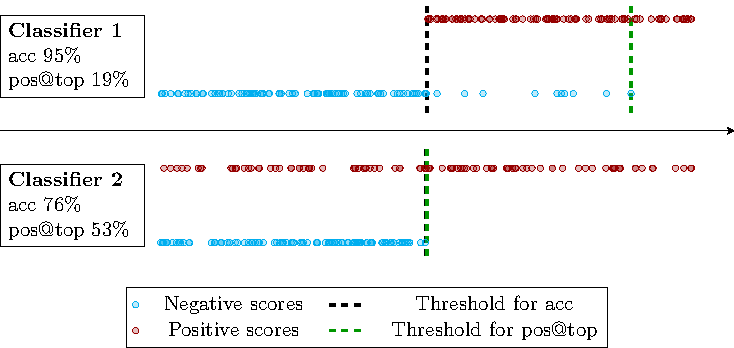
\includegraphics{images/standard_aatp_comparison.pdf}
  \caption{Difference between standard classifiers (\textbf{Classifier~1}) and classifiers maximizing~$\postop$ metric (\textbf{Classifier~2}). While the former has a good total accuracy, the latter has a good~$\postop$ metric.}
  \label{fig: standard vs. aatp}
\end{figure}

\begin{figure}
  \centering
  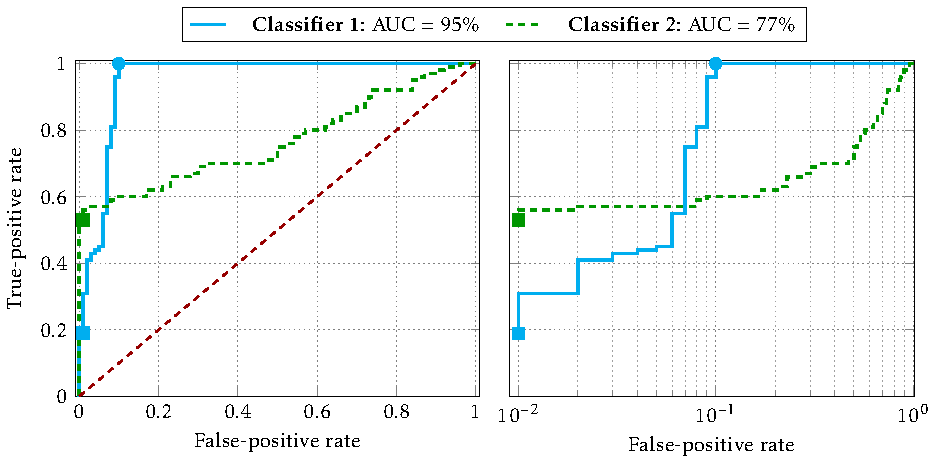
\includegraphics{images/roc_space_log.pdf}
  \caption{Difference between standard classifiers (\textbf{Classifier~1}) and classifiers maximizing~$\postop$ metric (\textbf{Classifier~2}). While the former has a good total accuracy, the latter has a good~$\postop$ metric.}
  \label{fig: roc space log}
\end{figure}

The rest of the chapter presents three main categories of problems that focus only on a small number of the most relevant samples. Moreover, in Chapter~\ref{chap: framework}, we show that at least some formulations from these three categories are closely related to binary classification.

\subsection{Ranking Problems}

The first category is the category of ranking problems. The ranking algorithms play a crucial role in many information retrieval problems:
\begin{itemize}
  \item \textbf{Document (Text) retrieval systems} are used for obtaining relevant documents from the collection of documents based on the relevance to the user's query. Such systems are widely used for accessing books, journals, or any other documents. However, the most visible application is search engines such as Google or DuckDuckGo.
  \item \textbf{Collaborative filtering} is one of the techniques used to predict the user's rating of a new product based on the past ratings of users with similar rating patter. Such systems can be used to generate music or video playlist automatically. Therefore, such systems are widely used in services such as Youtube or Spotify.
\end{itemize}
The two examples above show that ranking problems usually depend on users' feedback or preferences. In binary classification, we have only the labels that represent if the samples are positive or negative. On the other hand, ranking problems use multiple ways to describe the users' feedback. One approach uses the feedback function~$\Phi: \R^d \times \R^d \to \R$ to represent the user's preferences~\cite{freund2003efficient}. In such a case, the feedback function can be defined for all pairs of samples~$(\bm{x}_i, \bm{x}_j)$ in the following way
\begin{equation*}
  \Phi(\bm{x}_i, \bm{x}_j) \; 
  \begin{cases}
    > 0 & \bm{x}_i \text{ is prefered over } \bm{x}_j, \\
    = 0 & \text{no preference,} \\
    < 0 & \bm{x}_j \text{ is prefered over } \bm{x}_i.
  \end{cases}
\end{equation*}
We can see, that the feedback function specify if the user prefers~$\bm{x}_i$ over~$\bm{x}_j$ or not. Moreover, the feedback function also specifies how strong the preference is, i.e., the higher the volume~$\abs{\Phi(\bm{x}_i, \bm{x}_j)},$ the higher the preference. Many ranking algorithms try to find some ordering of all samples that minimizes the number of incorectly ordered pairs of samples. Consider ranking function~$r: \R^d \to \R.$ The sample~$\bm{x}_i$ is ranked higher than sample~$\bm{x}_j$ if~$r(\bm{x}_i) > r(\bm{x}_j).$ Then, the minimization of the number of misordered pairs can be formally written as follows
\begin{mini}{r}{
  \sum_{i \in \I} \sum_{j \in \I} \Iverson{r(\bm{x}_i) \leq r(\bm{x}_j)} \cdot \max\Brac[c]{0, \; \Phi(\bm{x}_i, \bm{x}_j)}.
  }{\label{eq: rankboost}}{}
\end{mini}
This problem is computationally demanding since the objective function contains a pairwise comparison of all samples. Therefore, the problem is not suitable for large data. \emph{RankBoost}~\cite{freund2003efficient} is an boosting algorithm based on the AdaBoost~\cite{freund1997decision} that combines many weak ordering functions to obtain the final ranking. This approach leads to the maximization of the area under the ROC curve~\cite{rudin2009pnorm}. Therefore, RankBoost focuses on the overall performance. However, as we discussed at the beginning of the section, we want to focus only on the small portion of the most relevant samples in many applications. In such a case, this approach is not ideal.

Consider recommendation of movies. In such a case, we only care about if the movie is good or not. It is not important if one bad movie is ranked higher than another bad movie. Both movies are still bad and therefore not relevant. Many ranking algorithms~\cite{rudin2009pnorm} use the so-called bipartite ranking to address this situation. In such a situation, each sample is positive (good) or negative (bad), and the goal is to push positive samples above negative ones. The authors of~\cite{rudin2009pnorm} proposed the following formulation
\begin{mini}{r}{
  \Brac{\sum_{j \in \Ineg} \Brac{\sum_{i \in \Ipos} \Iverson{r(\bm{x}_i) \leq r(\bm{x}_j)}}^p}^{\frac{1}{p}}.
  }{\label{eq: p-norm push}}{}
\end{mini}
The authors of~\cite{rudin2009pnorm} also proposed boosting algorithm called \textbf{$p$-Norm Push} to solve the formulation above. Note that for~$p = 1$, the formulation~\eqref{eq: p-norm push} is very similar to the RankBoost~\eqref{eq: rankboost}. In such a case, the resulting ranking function maximizes the AUC and therefore focuses on optimizing overall rankig. On the other hand, for~$p \rightarrow +\infty$, the formulation~\eqref{eq: p-norm push} minimizes the largest number of positive samples ranked below any negative sample
\begin{mini*}{r}{
  \max_{j \in \Ineg} \; \sum_{i \in \Ipos} \Iverson{r(\bm{x}_i) \leq r(\bm{x}_j)}.
  }{}{}
\end{mini*}
In such a case, the resulting ranking function focus only on the absolute top, i.e., it aims to push as many positive samples above the negative sample with the highest rank. Moreover, the formulation above can be equivalently rewritten as follows
\begin{mini}{r}{
  \sum_{i \in \Ipos} \Iverson{r(\bm{x}_i) \leq \max_{j \in \Ineg} \; r(\bm{x}_j)}.
  }{\label{eq: toppush rank}}{}
\end{mini}
Authors of~\cite{agarwal2011infinite} focus on this formulation and introduces SVM (\emph{Support Vector Machines}~\cite{cortes1995support}) based algorithm called \emph{Infinite Push} to solve it. Finally, authors of~\cite{li2014top} proposed an even more efficient algorithm with the linear complexity in the number of samples called \TopPush. Note that the objective function of the problem above is almost the same as the metric~\eqref{eq: metric pos at top}. Therefore, this \textbf{Classifier 2} from Figures~\ref{fig: standard vs. aatp} and~\ref{fig: roc space log} corresponds to the ranking function given by \TopPush algorithm. It shows a tied connection between binary classification and the bipartite ranking problems. 

\subsection{Accuracy at the Top}

In the previous section, we introduced formulation~\eqref{eq: toppush rank}, which focuses on maximizing the number of positive samples above the worst negative sample (the one with the highest rank or highest classification score). This formulation is very useful, as discussed at the beginning of this section. However, such a maximization problem can be unstable since the objective function does not allow false-positive errors. Therefore, if there is one negative outlier with a high score, the number of positive samples above this outlier can be tiny. The authors of~\cite{boyd2012accuracy} focus on similar problems as \TopPush, but use a different approach. They proposed the following formulation and it called \textbf{Accuracy at the Top}
\begin{mini}{\bm{w}}{
  \frac{1}{\nneg} \fp(\bm{s}, t) + \frac{1}{\npos} \fn(\bm{s}, t)
  }{\label{eq: aatp intro}}{}
  \addConstraint{s_i}{= f(\bm{x}_i; \bm{w}), \quad i \in \I}
  \addConstraint{t}{= \max \Set{t}{\frac{1}{\nall} \sum_{i \in \I} \Iverson{s_i \geq t} \geq \tau},}
\end{mini}
where~$f: \R^d \to \R$ is a model. This formulation focuses on the top $\tau$-fraction of all samples and tries to maximize the number of positive samples and minimize the number of negative samples in it. Even though the goal is to maximize the number of positive samples above the top $\tau$-quantile, the objective function contains false-positive and false-negative rates. It should be sufficient to include only one of them since the definition of the threshold implies the minimization of the other one as well. However, this form of objective function should be more robust~\cite{grill2016learning}. The problem of Accuracy at the Top is useful, for example, in applications where identified samples undergo expensive post-processing, such as human evaluation. For example, potentially useful drugs need to be preselected and manually investigated in drug development. Since the manual investigation is costly, we have to select only a fraction of drugs with the highest potential. However, it is precisely what Accuracy at the Top does.

There are many methods on how to solve Accuracy at the Top, since the formulation is complicated due to the top $\tau$-quantile in the constraint. The early approaches aim at solving approximations. For example, the authors of \cite{joachims2005svm} optimize a convex upper bound on the number of errors among the top samples. Due to exponentially many constraints, the method is computationally expensive. In \cite{boyd2012accuracy} the authors presented an SVM-like formulation. They assume that the top $\tau$-quantile is one of the samples, construct~$n$ unconstrained optimization problems with fixed thresholds, solve them and select the best solution. While this removes the necessity to handle the (difficult) quantile constraint, the algorithm is computationally infeasible for a large number of samples. The authors of~\cite{grill2016learning} proposed the projected gradient descent method, where after each gradient step, the quantile is recomputed. In \cite{eban2017scalable} authors suggested new formulations for various criteria and argued that they keep desired properties such as convexity. Finally, the authors of~\cite{tasche2018plug} showed that Accuracy at the Top is maximized by thresholding the posterior probability of the relevant class.

\subsection{Hypothesis Testing}

The hypothesis testing operates with null~$H_0$ and alternative~$H_1$ hypothesis. The goal is to either reject the null hypothesis in favor of the alternative or not to reject it. Since this problem is binary, two possible errors can occur. Type I occurs when~$H_0$ is true but is rejected, and Type II error happens when~$H_0$ is false but fails to be rejected. The Neyman-Pearson problem minimizes~\cite{neyman1933ontheproblem} Type II error while keeping Type I error smaller than some predefined bound. Using our notation for the Neyman-Pearson problem, the null hypothesis~$H_0$ states that sample~$\bm{x}$ has a negative label. Then Type I error occurs when the sample is false-positive, while Type II error occurs when the sample is false-negative. Therefore, the Neyman-Pearson problem minimizes the false-negative rate with the prescribed level~$\tau$ of the false-positive rate. Such constraint can be written in the form of quantile, i.e., the threshold is the top $\tau$-quantile of scores of all negative samples.
\begin{mini*}{f}{
  \frac{1}{\npos} \fn(\bm{s}, t)
  }{}{}
  \addConstraint{s_i}{= f(\bm{x}_i), \quad i \in \I}
  \addConstraint{t}{= \max \Set{t}{\frac{1}{\nneg} \sum_{i \in \Ineg} \Iverson{s_i \geq t} \geq \tau},}
\end{mini*}
This formulation is very similar to the one for Accuracy at the Top~\eqref{eq: aatp intro}. The main difference is that the quantile in the constraint is not computed from all but only from negative samples. Also, note one key difference in interpretation. The~$\tau$ in Accuracy at the Top represents the total amount of samples we want to process with the smallest possible error. On the other hand, in the Neyman-Pearson problem~$\tau$ represents the maximal acceptable false-positive rate. Therefore, the former approach is useful in situations where we can process only a certain number of samples. The latter is for situations where we have strict constraints on false-positive errors.

\section{Summary}

In this chapter, we introduced the general formulation~\eqref{eq: Binary classification counts} for binary classification and discussed how to measure the performance of binary classifiers. The first approach for performance evaluation is based on the confusion matrix. This approach is very straightforward. Moreover, it is possible to derive many different classification matrices from the confusion matrix. Table~\ref{tab: classification metrics} summarizes classification matrices derived from the confusion matrix used in the upcoming chapters. The second approach introduced in this chapter uses the ROC space to visualize the ability of classifiers to rank positive samples above negative ones. Since standard binary classification focuses on optimizing the overall performance, we discussed that there are many problems closely tied to the binary classification that focuses on the performance only of the most relevant samples. Such problems occur in many applications, from search engines to drug development. We also introduced Ranking problems, the problem of Accuracy at the Top, and the Neyman-Pearson problem and discussed their relation to the binary classification.

In the upcoming chapters, we focus on these three groups of problems and introduce a general framework to handle them. More precisely, the rest of the text is organized as follows.
\begin{itemize}
  \item Chapter~\ref{chap: framework} introduces a general optimization framework for classification at the top. Many problems fall into this framework even though they are usually considered separate problems. We describe Ranking problems, Accuracy at the Top, and the Neyman-Pearson problem in more detail and show that many formulations from these three categories fall into the framework. Moreover, we derive two new formulations closely related to the existing one. Finally, we discussed the basic properties and relations between introduced formulations. All formulations are introduced in a general form with arbitrary model~$f$, even though many of them have been initially designed only for a linear model. Theoretical properties of the formulations with different models are discussed later.
  \item Chapter~\ref{chap: linear} is dedicated to the linear model and formulations in their primal form, i.e., in the form presented in this chapter. This chapter shows that some formulations have nice properties such as convexity, differentiability, or stability. We derive some theoretical guarantees for the optimal solution based on these properties.
  \item Chapter~\ref{chap: dual} is dedicated to the dual forms of formulations from Table~\ref{tab: summary formulations}. In this chapter, we again assume a linear model only and show that all formulations can be split into two families based on their similarities. Then we derive dual formulations for these two families and show that these formulations are very similar to standard SVM. Using this observation, we use kernel trick to employ non-linearity into the formulations. Finally, we derive an efficient algorithm for solving the formulations.
  \item In Chapter~\ref{chap: deep}, we assume a nonlinear model. A prototypical example of such a model can be a neural network. The resulting formulations are not decomposable since the decision threshold is always a function of all classification scores. Therefore, it is impossible to use the stochastic descent algorithm directly to solve them. In Chapter~\ref{chap: deep}, we present two approaches to deal with this problem.
  \item Chapter~\ref{chap: experiments} is dedicated to all numerical experiments.
  \item Chapter~\ref{chap: experiments} summarizes all results presented in this work. 
\end{itemize}
Chapter~\ref{chap: framework} is crucial for the whole work since it introduces all formulations that are studied in the rest of the work. On the other hand, Chapters~\ref{chap: linear}, \ref{chap: dual}, and~\ref{chap: deep} study the properties of these formulations in three different settings. Therefore, these three chapters can be read separately. 

\begin{note}
  To improve the readability of the main part of the work, we postpone many results into appendices. Main results are presented in the main part, but all auxiliary results and proofs are located in appendices.
\end{note}

\chapter{Binary Classiciation at the Top}\label{chap: framework}

In the previous chapter, we introduced the general formulation of the binary classification problem~\eqref{eq: Binary classification counts} and basic ways how to evaluate the performance of binary classification. Furthermore, we introduced three problems that are closely related to binary classification, but focus on specific performance criteria. Namely: accuracy at the top, ranking problems and problem of hypothesis testing. Eventhough these problems are usually considered separately, they have one important thing in common: all three problems can be formulated as a minimization of the number of misclassified samples below (or above) a certain threshold. More specifically, in the rest of the chapter we show, that all mentioned problems falls into the following unified framework
\begin{mini}{\bm{w}}{
  \lambda_1 \cdot \fp(\bm{s}, t) + \lambda_2 \cdot \fn(\bm{s}, t)
}{\label{eq: aatp counts}}{}
  \addConstraint{s_i}{= f(\bm{x}_i; \bm{w}), \quad}{i \in \I}
  \addConstraint{t}{= G\Brac{\Brac[c]{(s_i, y_i)}_{i \in \I}},}
\end{mini}
where function~$G \colon \R^n \times \{0, 1\}^n \to \R$ takes the scores and labels of all samples and computes the decision threshold. In other words, all mentioned problems can be formulated as a binary classification problem with special condition on the decision threshold. Then the problems only differ in the way they define the function~$G$. The important distinction from standard binary classification is that the decision threshold is no longer fixed (as in case of neural networks) or trained independently (as in case of SVM), but is a function of scores of all samples. Therefore, the minimization in the problem~\eqref{eq: aatp counts} is performed only with respect to the one variable~$\bm{w}$.

The problem~\eqref{eq: aatp counts} is difficult to handle, since the objective function contains Iverson function~\eqref{eq: iverson} and therefore is discontinuous. The usual approach how to get a continuous objective function is to employ a surrogate function to replace the Iverson function~\cite{li2014top, grill2016learning}.

\begin{notation}[Surrogate function]\label{not: surrogates}
  In the text below, the symbol~$l$ denotes any convex non-negative non-decreasing function with~$l(0) = 1$. As examples of such function we can mention the hinge loss function or the quadratic hinge loss functions defined as follows
  \begin{equation*}
    \begin{aligned}
      l_{\text{hinge}}(s) & = \max\Brac[c]{0, 1 + s}, \\
      l_{\text{quadratic}}(s) & = \Brac{\max\Brac[c]{0, 1 + s}}^2.\\
    \end{aligned}
  \end{equation*}
  We also use parameter~$\vartheta > 0$ to scale inputs to the surrogate functions.
\end{notation}

Figure~\ref{fig: surrogates} compares Iverson function with hinge loss and quadratic hinge loss with different scaling parameters. As can be seen, the surrogate function always provides an upper approximation of the Iverson function, i.e.~$l(s) \geq \Iverson{s \geq 0}$ for all~$s \in \R.$ Besides that, if the scaling parameter is larger than 1, then the surrogate functions approximate the Iverson function better on the interval~$(-\infty, 0]$. However, the approximation on the interval~$[0, \infty)$ is worse. Even though the scaling parameter affects a lot the quality of the approximation, the usual choice is 1.

\begin{figure}[t]
  \centering
  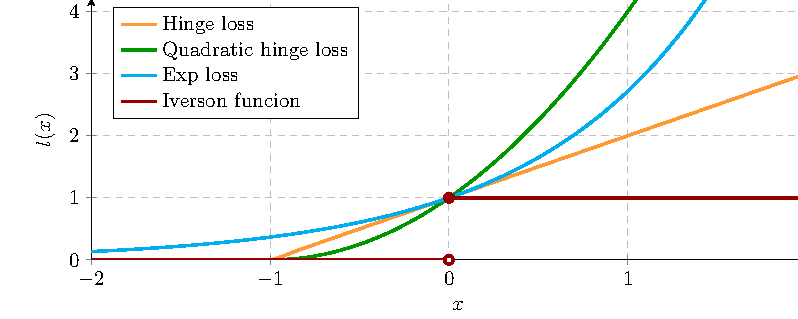
\includegraphics[width = \linewidth]{images/surrogates.pdf}
  \caption{Surrogates}
  \label{fig: surrogates}
\end{figure}

To follow the notation from the previous chapter, we define surrogate approximations of the counts defined in equation~\eqref{eq: confusion counts}. Using surrogate function~$l$ that fulfill the requirements mentioned in Notation~\ref{not: surrogates}, the counts~\eqref{eq: confusion counts} may be approximated by their surrogate counterparts defined as follows
\begin{equation}\label{eq: confusion counts surrogate}
  \begin{aligned}
    \tps(\bm{s}, t) & = \sum_{i \in \Ipos}l(s_i - t), & \qquad
    \fns(\bm{s}, t) & = \sum_{i \in \Ipos}l(t - s_i), \\
    \tns(\bm{s}, t) & = \sum_{i \in \Ineg}l(t - s_i), &
    \fps(\bm{s}, t) & = \sum_{i \in \Ineg}l(s_i - t).
  \end{aligned}
\end{equation}
Since the surrogate function provides upper approximation of the Iverson function, the surrogate counts~\eqref{eq: confusion counts surrogate} provide upper approximations of the true counts~\eqref{eq: confusion counts}. Replacing the counts in~\eqref{eq: aatp counts} by their surrogate counterparts and adding a regularization results in
\begin{mini}{\bm{w}}{
  \frac{1}{2} \norm{\bm{w}}^2 + \lambda_1 \cdot \fps(\bm{s}, t) + \lambda_2 \cdot \fns(\bm{s}, t)
  }{\label{eq: aatp surrogate}}{}
  \addConstraint{s_i}{= f(\bm{x}_i; \bm{w}), \quad i \in \I}
  \addConstraint{t}{= G\Brac{\Brac[c]{(s_i, y_i)}_{i \in \I}}.}
\end{mini}
The regularization is not necessary, but it is usually added for better numerical stability. The resulting optimization problem is easier to solve than problem~\eqref{eq: aatp counts} since the objective function is continuous. To derive other theoretical properties, we need to know the concrete form of the decision threshold function~$G$ as well as the form of the used model~$f.$ Different forms of the function~$G$ are discussed in the rest of this chapter and different forms of model~$f$ in Chapters~\ref{chap: linear} - \ref{chap: deep}.

In the rest of the chapter, we show, that accuracy at the top, ranking problems and the problem of hypothesis testing can be formulated in such a way, that fall  into our general framework of~\eqref{eq: aatp counts} or to its surrogate approximation~\eqref{eq: aatp surrogate}. Most of the problems that we refer to are originally defined for the linear model only, i.e. for~$f(\bm{x}; \bm{w}) = \bm{w}^{\top} \bm{x}.$ However, we formulate all the problems for general model~$f$ and then in Chapters~\ref{chap: linear} - \ref{chap: deep} we discuss their properties based on the used model. 

\begin{notation}[Classification scores]\label{not: scores}
  In Notation~\ref{not: classifier}, we defined vector~$\bm{s} \in \R^n$ of scores of all samples with components defined as
  \begin{equation*}
    s_i = f(\bm{x}_i; \bm{w}), \quad i \in \I,
  \end{equation*}
  where~$f \colon \R^d \to \R$ represents arbitrary model. To simplify the upcoming sections, we define sorted version of the vector of scores~$\bm{s}_{[\cdot]}$ with decreasing components, i.e.
  \begin{equation*}
    s_{[1]}   \geq s_{[2]} \geq \dots \geq s_{[n - 1]} \geq s_{[n]}.
  \end{equation*}
  Moreover, we denote negative samples as~$\bm{x}^-$ and positive samples as~$\bm{x}^+.$ Finally, we define vectors~$\bm{s}^- \in \R^{\nneg},$ $\bm{s}^+ \in \R^{\npos}$ of scores of all positive and negative samples with components defined as
  \begin{equation*}
    \begin{aligned}
      s^-_i & = f(\bm{x}^-_i; \bm{w}), \quad i = 1, \; 2, \ldots, \; \nneg, \\
      s^+_i & = f(\bm{x}^+_i; \bm{w}), \quad i = 1, \; 2, \ldots, \; \npos,
    \end{aligned}
  \end{equation*}
  and their sorted versions~$\bm{s}^-_{[\cdot]}$, $\bm{s}^+_{[\cdot]}$ with decreasing components.
\end{notation}

\section{Ranking problems}\label{sec: ranking}

The first category of formulations falling into our framework~\eqref{eq: aatp counts} and~\eqref{eq: aatp surrogate} are ranking methods which attempt to put as many positive (relevant) samples to the top as possible. The number of positive samples on top equals to the number of positive samples with classification score equal or larger than the highest classicication score corresponding to negative sample. This amounts to maximizing the number of true-positive samples or, equivalently, minimizing the number of false-negative negative samples, which may be written as
\begin{mini}{\bm{w}}{
  \frac{1}{\npos} \fn(\bm{s}, t)
  }{\label{eq: toppush}}{}
  \addConstraint{s_i}{= f(\bm{x}_i; \bm{w}), \quad i \in \I}
  \addConstraint{t}{= s_{[1]}^-}
\end{mini}
Since the threshold~$t$ is a function of score, the problem~\eqref{eq: toppush} is a special case of~\eqref{eq: aatp counts} for~$\lambda_1 = 0$ and~$\lambda_2 = \nicefrac{1}{\npos}$. The authors in~\cite{li2014top} proposed an efficient method to solve the formulation above and called it \TopPush. They replaced the number of false-negative samples with its surrogate counterpart in the objective function of~\eqref{eq: toppush} and added the regularization term to arrive at
\begin{mini}{\bm{w}}{
  \frac{1}{2} \norm{\bm{w}}^2 + \frac{1}{\npos} \fns(\bm{s}, t)
  }{\label{eq: toppush surrogate}}{}
  \addConstraint{s_i}{= f(\bm{x}_i; \bm{w}), \quad i \in \I}
  \addConstraint{t}{= s_{[1]}^-}
\end{mini}
Similarly to the original problem, this surrogate approximation falls into our framework of~\eqref{eq: aatp surrogate} for~$\lambda_1 = 0$ and~$\lambda_2 = \nicefrac{1}{\npos}$. However, \TopPush can be very sensitive to outliers. Especially when the linear model is used, as shown in Section~\ref{sec: stability}. To robustify \TopPush formulation, we follow the idea from~\cite{lapin2015top} and propose to replace the largest negative score by the mean of~$K$ largest negative scores. We call this approach \TopPushK and the resulting formulation is as follows
\begin{mini}{\bm{w}}{
  \frac{1}{2} \norm{\bm{w}}^2 + \frac{1}{\npos} \fns(\bm{s}, t)
  }{\label{eq: toppushK surrogate}}{}
  \addConstraint{s_i}{= f(\bm{x}_i; \bm{w}), \quad i \in \I}
  \addConstraint{t}{= \sum_{i = 1}^{K} s_{[i]}^-},
\end{mini}
where we use Notation~\ref{not: scores}. We used the mean of highest~$K$ negative scores instead of the value of the~$K$-th negative score to preserve convexity as shown in Section~\ref{sec: convexity}. 

\section{Accuracy at the Top}\label{sec: aatp}

The previous category considers formulations which minimize the number of positive samples below the highest-ranked negative sample, i.e. minimize the number of false-negative samples. Accuracy at the Top~\cite{boyd2012accuracy} takes a different approach and minimizes the number of negative samples with the score above the top~$\tau$-quantile of all scores defined by
\begin{equation}\label{eq: aatp quantile} 
  t_1(\bm{s})
    = \max \Set{t}{\frac{1}{n} \sum_{i \in \I} \Iverson{s_i \geq t} \geq \tau}.
\end{equation}
Then the Accuracy at the Top problem is defined by
\begin{mini}{\bm{w}}{
  \frac{1}{\nneg} \fp(\bm{s}, t)
  }{\label{eq: aatp original}}{}
  \addConstraint{s_i}{= f(\bm{x}_i; \bm{w}), \quad i \in \I}
  \addConstraint{t}{= \max \Set{t}{\frac{1}{n} \sum_{i \in \I} \Iverson{s_i \geq t} \geq \tau}}{~}
\end{mini}
This formulation already falls into our framework~~\eqref{eq: aatp counts} for~$\lambda_1 = \nicefrac{1}{\nneg}$ and~$\lambda_2 = 0$. However, this formulation can be rewritten using the following lemma.
\begin{restatable}{lemma}{lemmaequivalence}\label{lemma:fnfp_equivalence}
  Denote by~$t$ the exact quantile from~\eqref{eq: aatp quantile}. Then for all~$\mu \in [0,1]$ we have
  \begin{equation}\label{eq: fn fp equivalence}
      \fp(\bm{s},t) = \mu \fp(\bm{s},t) + (1-\mu)\fn(\bm{s},t) + (1-\mu)(n\tau - \npos) + (1-\mu)(q - 1),
  \end{equation}
  where~$q$ represents the number of samples which score is equal to~$t$
  \begin{equation*}
      q := \# \Set{i \in \I}{ \bm{s}_i = t}.
  \end{equation*}
\end{restatable}
\noindent The previous lemma can be used to replace the objective function in~\ref{eq: aatp original}. The right-hand side of~\eqref{eq: fn fp equivalence} consists of three parts. The first one is a convex combination of false-positive and false-negative counts. The second one is a constant term which has no impact on optimization. Finally, the third term~$(1-\mu)\Brac{q - 1}$ equals the number of samples for which their score equals the quantile. However, this term is small in comparison with the true-positive and the false-negative counts and can be neglected. Moreover, when the data are ``truly'' random such as when measurement errors are present, then~$q = 1$ and this term vanishes completely. Altogether, we get the following (almost) equivalent formulation to the problem~\eqref{eq: aatp original}
\begin{mini}{\bm{w}}{
  \mu \fp(\bm{s},t) + (1 - \mu)\fn(\bm{s},t)
  }{\label{eq: aatp original combination}}{}
  \addConstraint{s_i}{= f(\bm{x}_i; \bm{w}), \quad i \in \I}
  \addConstraint{t}{= \max \Set{t}{\frac{1}{n} \sum_{i \in \I} \Iverson{s_i \geq t} \geq \tau},}{~}
\end{mini}
where~$\mu \in [0,1]$. This problem with~$\mu = 0$ equals to~\eqref{eq: aatp original}, while with~$\mu = \nicefrac{\nneg}{n}$ it corresponds to the original definition (without regularization) from~\cite{boyd2012accuracy}.

Paper~\cite{grill2016learning} builds on the Accuracy at the Top problem~\eqref{eq: aatp original combination}, where it replaces false-positive and false-negative counts in the objective function by their surrogate counterparts. This leads to
\begin{mini}{\bm{w}}{
  \frac{1}{2} \norm{\bm{w}}^2 + \frac{1}{\nneg}\fps(\bm{s}, t) + \frac{1}{\npos} \fns(\bm{s}, t)
  }{\label{eq: grill}}{}
  \addConstraint{s_i}{= f(\bm{x}_i; \bm{w}), \quad i \in \I}
  \addConstraint{t}{= \max \Set{t}{\frac{1}{n} \sum_{i \in \I} \Iverson{s_i \geq t} \geq \tau}.}{~}
\end{mini}
Based on the first author, we name this formulation \Grill. This formulation falls into our framework~\eqref{eq: aatp surrogate} for~$\lambda_1 = \nicefrac{1}{\nneg}$ and~$\lambda_2 = \nicefrac{1}{\npos}$.

Apart from the quantile~\eqref{eq: aatp quantile}, there are two other possible choices of the threshold. The first on is simple approximation of the the true quantile by mean of the~$n\tau$ largest scores 
\begin{equation}\label{eq: aatp quantile mean} 
  t_2(\bm{s}) = \frac{1}{n\tau} \sum_{i=1}^{n\tau} s_{[i]}.
\end{equation}
where for simplicity we assume, that~$n\tau$ is an integer. The quantile~\eqref{eq: aatp quantile} is sometimes denoted as VaR (value at risk) and the quantile~\eqref{eq: aatp quantile mean} as CVaR (conditional value of risk).The main purpose of~\eqref{eq: aatp quantile mean} is to provide a convex approximation of the non-convex quantile~\eqref{eq: aatp quantile}. In fact, it is known is that it is the tightest convex approximation of~\eqref{eq: aatp quantile}. Putting~\eqref{eq: aatp quantile mean} into the constraint results in the following problem, which we call \TopMeanK
\begin{mini}{\bm{w}}{
  \frac{1}{2} \norm{\bm{w}}^2 + \frac{1}{\npos} \fns(\bm{s}, t)
  }{\label{eq: topmeank}}{}
  \addConstraint{s_i}{= f(\bm{x}_i; \bm{w}), \quad i \in \I}
  \addConstraint{t}{= \frac{1}{K} \sum_{i=1}^{K} s_{[i]},}
\end{mini}
where~$K = n\tau.$ Note that this formulation is very similar to the \TopPushK formulation from the previous section. The only difference is, that the threshold is computed from scores of all samples and not only from the negative ones as for \TopPushK. 

The second option how to approximate the true qunatile~\eqref{eq: aatp quantile} is to use surrogate counterparts to replace counts in~\eqref{eq: aatp quantile} and solve the following equality
\begin{equation}\label{eq: aatp quantile surrogate}
  t_3(\bm{s}) \quad \text{solves} \quad \frac{1}{n}\sum_{i \in \I} l\Brac{\vartheta(s_i - t)} = \tau, 
\end{equation}
where~$\vartheta > 0$ is scaling parameter.Since this threshold uses the surrogate approximation, we will sometimes denote it as surrogate top~$\tau$-quantile. Similarly to the previous case, we can use the surrogate top~$\tau$-quantile in the constraint to arrive at
\begin{mini}{\bm{w}}{
  \frac{1}{2} \norm{\bm{w}}^2 + \frac{1}{\npos} \fns(\bm{s}, t)
  }{\label{eq: patmat}}{}
  \addConstraint{s_i}{= f(\bm{x}_i; \bm{w}), \quad i \in \I}
  \addConstraint{t}{\quad \text{solves} \quad \frac{1}{n}\sum_{i \in \I} l\Brac{\vartheta(s_i - t)} = \tau.}
\end{mini}
Note that \Grill minimizes the convex combination of false-positives and false-negatives while~\eqref{eq: topmeank} and~\eqref{eq: patmat} minimize only the false-negatives. The reason for this will be evident in Section~\ref{sec: convexity} and amounts to preservation of convexity for linear model. Moreover, problem~\eqref{eq: patmat} provides a good approximation to the Accuracy at the Top problem and for linear model is easily solvable due to convexity and requires almost no tuning. For this reason we named it \PatMat (Precision At the Top \& Mostly Automated Tuning).

\section{Neyman-Pearson problem}\label{sec: Neyman-Pearson}

Another category falling into the framework of~\eqref{eq: aatp counts} and~\eqref{eq: aatp surrogate} is the Neyman-Pearson problem which is closely related to hypothesis testing, where null~$H_0$ and alternative~$H_1$ hypotheses are given. Type~I error occurs when~$H_0$ is true but is rejected, and Type II error happens when~$H_0$ is false, but it fails to be rejected. The standard technique is to minimize Type II error while a bound for Type I error is given.

In the Neyman-Pearson problem, the null hypothesis~$H_0$ states that a sample~$\bm{x}$ has the negative label. Then Type I error occurs when the sample is false-positive while Type II error when the sample is false-negative, see Table~\ref{tab: classification metrics}. In other words, minimizing Type II error corresponds to minimizing the number of false-negative samples and the bound for Type I error is equivalent to the bound on the number of false-positive samples, i.e. if the bound on Type I error equals~$\tau$, we may write this as
\begin{equation}\label{eq: NP quantile} 
  t_1^{\rm NP}(\bm{s})
    = \max \Set{t}{\fp(\bm{s}, t) \geq \nneg \tau}
    = \max \Set{t}{\frac{1}{\nneg} \sum_{i \in \Ineg} \Iverson{s_i \geq t} \geq \tau}.
\end{equation}
Note that in~\eqref{eq: NP quantile} we only count the false-positive samples instead of counting all positives in~\eqref{eq: aatp quantile}. Then, we may write the Neyman-Pearson problem as
\begin{mini}{\bm{w}}{
  \frac{1}{\npos} \fn(\bm{s}, t)
  }{\label{eq: NP problem}}{}
  \addConstraint{s_i}{= f(\bm{x}_i; \bm{w}), \quad i \in \I}
  \addConstraint{t}{= \max \Set{t}{\frac{1}{\nneg} \sum_{i \in \Ineg} \Iverson{s_i \geq t} \geq \tau}.}{~}
\end{mini}
This problem again falls within our framework for~\eqref{eq: aatp counts} for~$\lambda_1 = 0$ and~$\lambda_2 = \nicefrac{1}{\npos}$. Since formulation~\eqref{eq: NP problem} and~\eqref{eq: aatp original combination} are almost identical, we can derive approximations of~\eqref{eq: NP problem} in the exactly the same way as in Section~\ref{sec: aatp}.

The first way how to approximate the formulation~\eqref{eq: aatp counts} is to replace the true counts  in the objective function by their surrogate counterparts as in~\cite{grill2016learning}. This results in the Neyman-Pearson variant of \Grill formulation. To emphasize this relationship, we call this formulation \GrillNP
\begin{mini}{\bm{w}}{
  \frac{1}{2} \norm{\bm{w}}^2 + \frac{1}{\nneg}\fps(\bm{s}, t) + \frac{1}{\npos} \fns(\bm{s}, t)
  }{\label{eq: grill np}}{}
  \addConstraint{s_i}{= f(\bm{x}_i; \bm{w}), \quad i \in \I}
  \addConstraint{t}{= \max \Set{t}{\frac{1}{\nneg} \sum_{i \in \Ineg} \Iverson{s_i \geq t} \geq \tau}.}{~}
\end{mini}
The second option is to use approximation of the true quantile. In such a case, the first choice is to replace the true qunatile by the mean of the~$\nneg\tau$ largest scores of negative samples 
\begin{equation}\label{eq: np quantile mean} 
  t_2^{\rm NP}(\bm{s}) = \frac{1}{\nneg\tau} \sum_{i=1}^{\nneg\tau} s^-_{[i]}.
\end{equation}
For simplicity, we again assume, that~$\nneg\tau$ is an integer. Putting~\eqref{eq: np quantile mean} into the constraint results in the the Neyman-Pearson alternative to \TopMeanK defined as
\begin{mini}{\bm{w}}{
  \frac{1}{2} \norm{\bm{w}}^2 + \frac{1}{\npos} \fns(\bm{s}, t)
  }{\label{eq: tau-fpl}}{}
  \addConstraint{s_i}{= f(\bm{x}_i; \bm{w}), \quad i \in \I}
  \addConstraint{t}{= \frac{1}{\nneg\tau} \sum_{i=1}^{\nneg\tau} s^-_{[i]}.}
\end{mini}
This problem already appeared in~\cite{zhang2018tau} under the name \tauFPL. We may see~\eqref{eq: tau-fpl} from two different viewpoints. First, for linear model \tauFPL provide convex approximations of \GrillNP as will be discussed in Chapter~\ref{chap: linear}. Second, \tauFPL has the same form as \TopPushK. The only difference is that for \tauFPL we have~$K = \nneg\tau$ while for \TopPushK the value of~$K$ is small. Thus, even though we started from two different problems, we arrived at two approximations which differ only in the value of one parameter. This shows a close relation of the ranking problem and the Neyman-Pearson problem and the need for a unified theory to handle these problems.

Finally, it is possible to use surrogate counterparts to replace counts in~\eqref{eq: NP quantile} and solve the following equality
\begin{equation}\label{eq: np quantile surrogate}
  t_3^{\rm NP}(\bm{s}) \quad \text{solves} \quad \frac{1}{\nneg}\sum_{i \in \Ineg} l\Brac{\vartheta(s_i - t)} = \tau. 
\end{equation}
This approximation of the true quantile leads to the Neyman-Pearson alternative to \PatMat in the following form
\begin{mini}{\bm{w}}{
  \frac{1}{2} \norm{\bm{w}}^2 + \frac{1}{\npos} \fns(\bm{s}, t)
  }{\label{eq: patmat np}}{}
  \addConstraint{s_i}{= f(\bm{x}_i; \bm{w}), \quad i \in \I}
  \addConstraint{t}{\text{solves} \quad \frac{1}{\nneg}\sum_{i \in \Ineg} l\Brac{\vartheta(s_i - t)} = \tau,}
\end{mini}
and we call it \PatMatNP.

\section{Summary}

\todo[inline]{Add summary of the framework and formulations that fall into the framework}

\begin{table}
  \centering
  \begin{NiceTabular}{lccccc}
    \toprule
    \textbf{Name}
      & \textbf{Definition}
      & \textbf{Source}
      & $\lambda_1$
      & $\lambda_2$
      & \textbf{Threshold} \\
    \midrule
    \TopPush
      & \eqref{eq: toppush surrogate}
      & \cite{li2014top}
      & 0
      & $\frac{1}{\npos}$
      & $s_{[1]}^-$ \\
    \TopPushK
      & \eqref{eq: toppushK surrogate}
      & ours~\cite{adam2021general}
      & 0
      & $\frac{1}{\npos}$
      & $\sum_{i = 1}^{K} s_{[i]}^-$ \\
    \midrule
    \Grill
      & \eqref{eq: grill}
      & \cite{grill2016learning}
      & $\frac{1}{\nneg}$
      & $\frac{1}{\npos}$
      & $\max \Set{t}{\frac{1}{n} \sum_{i \in \I} \Iverson{s_i \geq t} \geq \tau}$ \\
    \TopMeanK
      & \eqref{eq: topmeank}
      & ---
      & 0
      & $\frac{1}{\npos}$
      & $\frac{1}{K} \sum_{i=1}^{K} s_{[i]}$ \\
    \PatMat
      & \eqref{eq: patmat}
      & ours~\cite{adam2021general}
      & 0
      & $\frac{1}{\npos}$
      & $\frac{1}{n} \sum_{i \in \I} l\Brac{\vartheta(s_i - t)} = \tau$ \\
    \midrule
    \GrillNP
      & \eqref{eq: grill np}
      & ---
      & $\frac{1}{\nneg}$ 
      & $\frac{1}{\npos}$
      & $\max \Set{t}{ \frac{1}{\nneg} \sum_{i \in \Ineg} \Iverson{s_i \geq t} \geq \tau}$ \\
    \tauFPL
      & \eqref{eq: tau-fpl}
      & \cite{zhang2018tau}
      & 0
      & $\frac{1}{\npos}$
      & $\frac{1}{\nneg\tau} \sum_{i=1}^{\nneg\tau} s^-_{[i]}$ \\
    \PatMatNP
      & \eqref{eq: patmat np}
      & ours~\cite{adam2021general}
      & 0
      & $\frac{1}{\npos}$
      & $\frac{1}{\nneg} \sum_{i \in \Ineg} l\Brac{\vartheta(s_i - t)} = \tau$ \\
    \midrule
    \emph{Precision@Recall}
      & (6) in~\cite{mackey2018constrained}
      & \cite{mackey2018constrained}
      & $\frac{1}{\nneg}$
      & 0
      & $\min \Set{t}{\frac{1}{\npos} \sum_{i \in \Ipos} s_i \leq \tau}$ \\
    \emph{Precision@K}
      & ---
      & ---
      & $\frac{1}{\nneg}$
      & 0
      & $s_{[K]}$ \\
      \emph{Recall@K}
      & ---
      & ---
      & 0
      & $\frac{1}{\npos}$
      & $s_{[K]}$ \\
    \bottomrule
  \end{NiceTabular}
  \caption{Summary of problem fomrulations that fall in the framework~\eqref{eq: aatp surrogate}. The  table shows their definition label, the source or the source they are based on, the values of parameters~$\lambda_1,$~$\lambda_2$ for framework~\eqref{eq: aatp surrogate} and the form of the decision threshold~$t$.}
  \label{tab: summary formulations}
\end{table}
\chapter{Linear Classification at the Top}

Many binary classification problems focus on separating the dataset by a linear hyperplane $\bm{w}^\top \bm{x} - t$. A sample $\bm{x}$ is deemed to be positive or relevant (depending on the application) if its score $\bm{w}^\top \bm{x}$ is above a threshold $t$. Multiple problem categories belong to this framework:
\begin{itemize}
  \item \textit{Ranking problems} select the most relevant samples and rank them. To each sample, a numerical score is assigned, and the ranking is performed based on this score. Often, only scores above a threshold are considered.
  \item \textit{Accuracy at the Top} is similar to ranking problems. However, instead of ranking the most relevant samples, it only maximizes the accuracy (equivalently minimizes the misclassification) in these top samples. The prime examples of both categories include search engines or problems where identified samples undergo expensive post-processing such as human evaluation.
  \item \textit{Hypothesis testing} states a null and an alternative hypothesis. The Neyman-Pearson problem minimizes the Type II error (the null hypothesis is false but it fails to be rejected) while keeping the Type I error (the null hypothesis is true but is rejected) small. If the null hypothesis states that a sample has the positive label, then Type II error happens when a positive sample is below the threshold and thus minimizing the Type II error amounts to minimizing the positives below the threshold.
\end{itemize}
Examples of this type can be found in search engines, where the user is interested only in the first few queries. These queries need to be of high quality. Other examples include cybersecurity~\cite{Grill_2016}, where a low false-negative rate is crucial as a high number of false alarms would result in the software being uninstalled, or drug development, where potentially useful drugs need to be preselected and manually investigated. All these three applications may be written (possibly after a reformulation) in a similar form as a minimization of the false-negatives (misclassified positives) above a threshold. They only differ in the way they define the threshold. Despite this striking similarity, they are usually considered separately in the literature. The main goal of this paper is to provide a unified framework for these three applications and perform its theoretical and numerical analysis.

The goal of the ranking problems is to rank the relevant samples higher than the non-relevant ones. A prototypical example is the RankBoost \cite{freund2003efficient} maximizing the area under the ROC curve, the Infinite Push \cite{agarwal2011infinite} or the $p$-norm push \cite{rudin.2009} which concentrate on the high-ranked negatives and push them down. Since all these papers include pairwise comparisons of all samples, they can be used only for small datasets. This was alleviated in \cite{Li_TopPush}, where the authors performed the limit $p \to \infty$ in $p$-norm push and obtained the linear complexity in the number of samples. Moreover, since the $l_{\infty}$-norm is equal to the maximum, this method falls into our framework with the threshold equal to the largest score computed from negative samples.

Accuracy at the Top ($\tau$-quantile) was formally defined in \cite{boyd2012accuracy} and maximizes the number of relevant samples in the top $\tau$-fraction of ranked samples. When the threshold equals the top $\tau$-quantile of all scores, this problem falls into our framework. The early approaches aim at solving approximations, for example, \cite{Joachims:2005:SVM:1102351.1102399} optimizes a convex upper bound on the number of errors among the top samples. Due to the presence of exponentially many constraints, the method is computationally expensive. \cite{boyd2012accuracy} presented an SVM-like formulation which fixes the index of the quantile and solves $n$ problems. While this removes the necessity to handle the (difficult) quantile constraint, the algorithm is computationally infeasible for a large number of samples. \cite{kar2015surrogate} derived upper approximations, their error bounds and solved these approximations. \cite{Grill_2016} proposed the projected gradient descent method where after each gradient step, the quantile is recomputed. \cite{Eban_2017} suggested new formulations for various criteria and argued that they keep desired properties such as convexity. \cite{tasche2018plug} showed that accuracy at the top is maximized by thresholding the posterior probability of the relevant class. The closest approach to our framework is \cite{lapin.2015,lapin2018analysis}, where the authors considered multi-class classification problems, and their goal was to optimize the performance on the top few classes and \cite{mackey2018constrained}, where the authors implicitly removed some variables and derived an efficient algorithm.

\section{Framework for Minimizing Missclassification Above a Threshold}\label{sec:framework}

Many important binary classification problems minimize the number of misclassified samples below (or above) certain threshold. Since these problems are usually considered separately, in this section, we provide a unified framework for their handling and present several classification problems falling into this framework.

For samples $\bm{x}$, we consider the linear classifier $f(\bm{w}) = \bm{w}^\top \bm{x} - t$, where $\bm{w}$ is the normal vector to the separating hyperplane and $t$ is a threshold. The most well-known example is the support vector machines, where $t$ is an optimization variable. In many cases the threshold $t$ is computed from the scores $s = \bm{w}^\top \bm{x}$. For example, \TopPush from \cite{Li_TopPush} sets the threshold $t$ to the largest score $s^-$ corresponding to negative samples and \cite{Grill_2016} sets it to the quantile of all scores.

To be able to determine the missclassification above and below the threshold $t$, we define the true-positive, false-negative, true-negative and false-positive counts by
\begin{equation}\label{eq:defin_counts}
  \begin{aligned}
    \tp(\bm{w}, t) & = \sum_{\bm{x} \in \Xc^+}\Brac[s]{\bm{w}^\top \bm{x} - t \ge 0}, &
    \fn(\bm{w}, t) & = \sum_{\bm{x} \in \Xc^+}\Brac[s]{\bm{w}^\top \bm{x} - t < 0}, \\
    \tn(\bm{w}, t) & = \sum_{\bm{x} \in \Xc^-}\Brac[s]{\bm{w}^\top \bm{x} - t < 0}, &
    \fp(\bm{w}, t) & = \sum_{\bm{x} \in \Xc^-}\Brac[s]{\bm{w}^\top \bm{x} - t \ge 0}.
  \end{aligned}
\end{equation}
Here $[\cdot]$ is the 0-1 loss (Iverson bracket, characteristic function) which is equal to $1$ if the argument is true and to $0$ otherwise. Moreover, $\Xc / \Xc^{+} / \Xc^{-}$ denotes the sets of all/positive/negative samples and by $n / n^{+} / n^{-}$ their respective sizes. 

Since the misclassified samples below the threshold are the false-negatives, we arrive at the following problem
\begin{equation}\label{eq:problem1}
  \begin{aligned}
    \minimize
    & \quad \frac{1}{n^{+}}\fn(\bm{w}, t)\\
    \st
    & \quad \text{threshold } t \text{ is a function of }\{\bm{w}^\top \bm{x}_i\}_{i = 1}^n.
  \end{aligned}
\end{equation}
As the 0-1 loss in \eqref{eq:defin_counts} is discontinuous, problem \eqref{eq:problem1} is difficult to handle. The usual approach is to employ a surrogate function such as the hinge loss function defined by
\begin{equation}\label{eq:defin_surrogate}
  \begin{aligned}
    l_{\rm hinge}(s) & =\max\Brac[c]{0, 1 + s}.\\
  \end{aligned}
\end{equation}
In the text below, the symbol $l$ denotes any convex non-negative non-decreasing function with $l(0) = 1$. Using the surrogate function, the counts \eqref{eq:defin_counts} may be approximated by their surrogate counterparts
\begin{equation}\label{eq:defin_counts_surr}
  \begin{aligned}
    \tps(\bm{w}, t) & = \sum_{\bm{x} \in \Xc^+}l(\bm{w}^\top \bm{x}-t), &
    \fns(\bm{w}, t) & = \sum_{\bm{x} \in \Xc^+}l(t - \bm{w}^\top \bm{x}), \\
    \tns(\bm{w}, t) & = \sum_{\bm{x} \in \Xc^-}l(t - \bm{w}^\top \bm{x}),&
    \fps(\bm{w}, t) & = \sum_{\bm{x} \in \Xc^-}l(\bm{w}^\top \bm{x}-t).
  \end{aligned}
\end{equation}
Since $l(\cdot)\ge[\cdot]$, the surrogate counts \eqref{eq:defin_counts_surr} provide upper approximations of the true counts \eqref{eq:defin_counts}. Replacing the counts in \eqref{eq:problem1} by their surrogate counterparts and adding a regularization results in
\begin{equation}\label{eq:problem2}
  \begin{aligned}
    \minimize
    & \quad \frac{1}{n^{+}}\fns(\bm{w}, t) + \frac{\lambda}{2}\norm{\bm{w}}^2 \\
    \st
    & \quad \text{threshold } t \text{ is a function of }\{\bm{w}^\top \bm{x}_i\}_{i = 1}^n.
  \end{aligned}
\end{equation}
In the rest of this section, we list formulations which fall into the framework of \eqref{eq:problem1} and \eqref{eq:problem2}.

\subsection{Methods based on pushing positives to the top}\label{sec:obj1}

The first category of formulations falling into our framework \eqref{eq:problem1} and \eqref{eq:problem2} are ranking methods which attempt to put as many positives (relevant samples) to the top as possible. Specifically, for each sample $\bm{x}$, they compute the score $s = \bm{w}^\top \bm{x}$ and then sort the vector $\bm{s}$ into $\bm{s}_{[\cdot]}$ with decreasing components $s_{[1]} \ge s_{[2]} \ge \dots \ge s_{[n]}$. The number of positives on top equals to the number of positives above the highest negative. This amounts to maximizing true-positives or, equivalently, minimizing false-negatives, which may be written as
\begin{equation}\label{eq:problem_top2}
  \begin{aligned}
    \minimize
    & \quad\frac{1}{n^{+}}\fn(\bm{w},t) \\
    \st
    & \quad t = s_{[1]}^-, \\
    & \quad \text{components of }\bm{s}^- \text{ equal to } s^- = \bm{w}^\top \bm{x}^-\text{ for }\bm{x}^- \in \Xc^-.
  \end{aligned}
\end{equation}
As $t$ is a function of the scores $s = \bm{w}^\top \bm{x}$, problem \eqref{eq:problem_top2} is a special case of \eqref{eq:problem1}.

\TopPush from \cite{Li_TopPush} replaces the false-negatives in \eqref{eq:problem_top2} by their surrogate and adds a regularization term to arrive at
\begin{equation}\label{eq:problem_toppush}
  \begin{aligned}
    \minimize
    & \quad \frac{1}{n^{+}} \fns(\bm{w}, t) + \frac{\lambda}{2} \norm{\bm{w}}^2 \\
    \st
    & \quad t = s_{[1]}^-, \\
    & \quad \text{components of }\bm{s}^-\text{ equal to } s^- = \bm{w}^\top \bm{x}^- \text{ for }\bm{x}^- \in \Xc^-.
  \end{aligned}
\end{equation}
Note that this falls into the framework of \eqref{eq:problem2}.

As we will show in Section \ref{sec:stability}, \TopPush is sensitive to outliers and mislabelled data. To robustify it, we follow the idea from \cite{lapin.2015} and propose to replace the largest negative score by the mean of $k$ largest negative scores. This results in
\begin{equation}\label{eq:problem_toppushk}
  \begin{aligned}
    \minimize
    & \quad \frac{1}{n^{+}} \fns(\bm{w}, t) + \frac{\lambda}{2} \norm{\bm{w}}^2 \\
    \st
    & \quad t = \frac{1}{k}(s_{[1]}^- + \dots + s_{[k]}^-), \\
    & \quad \text{components of } \bm{s}^- \text{ equal to } s^-= \bm{w}^\top \bm{x}^- \text{ for }\bm{x}^- \in \Xc^-.
  \end{aligned}
\end{equation}
We used the mean of highest $k$ negative scores instead of the value of the $k$-th negative score to preserve convexity as shown in Section \ref{sec:convexity}.

\subsection{Accuracy at the Top}\label{sec:obj2}

The previous category considers formulations which minimize the false-negatives below the highest-ranked negative. Accuracy at the Top \cite{boyd2012accuracy} takes a different approach and minimizes false-positives above the top $\tau$-quantile defined by
\begin{equation}\label{eq:defin_quantile} 
  t_1(\bm{w}) = \max \Brac[c]{t \mid \tp(\bm{w}, t) + \fp(\bm{w}, t) \ge n \tau}.
\end{equation}
Then the Accuracy at the Top problem is defined by
\begin{equation}\label{eq:problem_aatp_orig}
  \begin{aligned}
    \minimize
    & \quad \frac{1}{n^{-}}\fp(\bm{w},t) \\
    \st
    & \quad t \text{ is the top \ensuremath{\tau}-quantile: it solves } \eqref{eq:defin_quantile}.
  \end{aligned}
\end{equation}
Due to Lemma \ref{lemma:fnfp_equivalence} in the Appendix, the previous problem \eqref{eq:problem_aatp_orig} is equivalent (up to a small theoretical issue) to
\begin{equation}\label{eq:problem_aatp}
  \begin{aligned}
    \minimize
    & \quad \mu \fn(\bm{w}, t) + (1 - \mu)\fp(\bm{w}, t) + \frac{\lambda}{2}\norm{\bm{w}}^2\\
    \st
    & \quad t\text{ is the top \ensuremath{\tau}-quantile: it solves }\eqref{eq:defin_quantile}
  \end{aligned}
\end{equation}
for any $\mu \in [0,1]$. This problem with $\mu = 0$ equals to \eqref{eq:problem_aatp_orig}, with $\mu = 1$ it falls into our framework \eqref{eq:problem1}, while with $\mu = \frac{n^-}{n}$ it corresponds to the original definition from \cite{boyd2012accuracy}. 

Apart from the quantile \eqref{eq:defin_quantile}, there are two other possible choices of the threshold
\begin{align}
  \label{eq:defin_quantile1} t_2(\bm{w}) =\ &\frac{1}{n\tau}\sum_{i=1}^{n\tau} s_{[i]}, \\
  \label{eq:defin_quantile0} t_3(\bm{w})\quad \text{solves} \quad & \frac{1}{n}\sum_{i = 1}^nl(\beta(s_i - t)) = \tau.
\end{align}
We again use the vector of scores $\bm{s}$ with components $s_i = \bm{w}^\top \bm{x}_i$ and for the rest of the paper we assume, for simplicity, that $n\tau$ is an integer. The quantile \eqref{eq:defin_quantile} is sometimes denoted as VaR (value at risk) and \eqref{eq:defin_quantile1} as CVaR (conditional value of risk). It is known is that the latter is the tightest convex approximation of the former. We will sometimes denote \eqref{eq:defin_quantile0} as surrogate top $\tau$-quantile. We will investigate the relations between these three objects as well as their properties such as convexity, differentiability or stability in Section \ref{sec:theory}.

Paper \cite{Grill_2016} builds on the Accuracy at the Top problem~\eqref{eq:problem_aatp}, where it replaces $\fn(\bm{w}, t)$ and $\fp(\bm{w}, t)$ in the objective by their surrogate counterparts $\fns(\bm{w}, t)$ and $\fps(\bm{w}, t)$. This leads to
\begin{equation}\label{eq:problem_grill}
  \begin{aligned}
    \minimize
    & \quad \frac{1}{n^{+}}\fns(\bm{w},t) + \frac{1}{n^{-}}\fps(\bm{w},t) + \frac{\lambda}{2}\norm{\bm{w}}^2\\
    \st
    & \quad t\text{ is the top \ensuremath{\tau}-quantile: it solves }\eqref{eq:defin_quantile}.
  \end{aligned}
\end{equation}
Based on the first author, we name this formulation \Grill. The main purpose of \eqref{eq:defin_quantile1} is to provide a convex approximation of the non-convex quantile \eqref{eq:defin_quantile}. Putting it into the constraint results in a convex approximation problem, which we call \TopMeanK
\begin{equation}\label{eq:problem_topmeank}
  \begin{aligned}
    \minimize
    & \quad \frac{1}{n^{+}} \fns(\bm{w},t) + \frac{\lambda}{2}\norm{\bm{w}}^2 \\
    \st
    & \quad t = \frac 1{n\tau}(s_{[1]} + \dots + s_{[n\tau]}), \\
    & \quad \text{components of }\bm{s}\text{ equal to } s = \bm{w}^\top \bm{x} \text{ for } \bm{x} \in \Xc.
  \end{aligned}
\end{equation}
Similarly, we can use the surrogate top quantile in the constraint to arrive at
\begin{equation}\label{eq:problem_patmat}
  \begin{aligned}
    \minimize
    & \quad \frac{1}{n^{+}} \fns(\bm{w},t) + \frac{\lambda}{2}\norm{\bm{w}}^2\\
    \st
    & \quad t \text{ is the surrogate top \ensuremath{\tau}-quantile: it solves }\eqref{eq:defin_quantile0}.
  \end{aligned}
\end{equation}
Note that \Grill minimizes the convex combination of false-positives and false-negatives while~\eqref{eq:problem_topmeank} and \eqref{eq:problem_patmat} minimize only the false-negatives. The reason for this will be evident in Section \ref{sec:convexity} and amounts to preservation of convexity. Moreover, as will see later, problem \eqref{eq:problem_patmat} provides a good approximation to the Accuracy at the Top problem, it is easily solvable due to convexity and requires almost no tuning, we named it \PatMat (Precision At the Top \& Mostly Automated Tuning). 

\subsection{Methods optimizing the Neyman-Pearson criterion}\label{sec:obj3}

Another category falling into the framework of \eqref{eq:problem1} and \eqref{eq:problem2} is the Neyman-Pearson problem which is closely related to hypothesis testing, where null $H_0$ and alternative $H_1$ hypotheses are given. Type~I error occurs when $H_0$ is true but is rejected, and type II error happens when $H_0$ is false, but it fails to be rejected. The standard technique is to minimize Type II error while a bound for Type I error is given.

In the Neyman-Pearson problem, the null hypothesis $H_0$ states that a sample $\bm{x}$ has the negative label. Then Type I error corresponds to false-positives while Type II error to false-negatives. If the bound on Type I error equals $\tau$, we may write this as
\begin{equation}\label{eq:defin_quantile_np} 
  t_1^{\rm NP}(\bm{w}) = \max\Brac[c]{t \mid \fp(\bm{w},t) \ge n^- \tau}.
\end{equation}
Then, we may write the Neyman-Pearson problem as
\begin{equation}\label{eq:problem_np}
  \begin{aligned}
    \minimize
    & \quad \frac{1}{n^{+}}\fn(\bm{w},t) \\
    \st
    & \quad t \text{ is Type I error at level \ensuremath{\tau}: it solves }\eqref{eq:defin_quantile_np}.
  \end{aligned}
\end{equation}
Since \eqref{eq:problem_np} differs from \eqref{eq:problem_aatp} only by counting only the false-positives in \eqref{eq:defin_quantile_np} instead of counting all positives in \eqref{eq:defin_quantile}, we can derive its approximations in exactly the same way as in Section \ref{sec:obj2}. We therefore provide only their brief description and start with approximations of \eqref{eq:defin_quantile_np}
\begin{align}
  \label{eq:defin_quantile1_np} t_2^{\rm NP}(\bm{w}) =\ &\frac{1}{n^-\tau}\sum_{i=1}^{n^-\tau} s_{[i]}^-, \\
  \label{eq:defin_quantile0_np} t_3^{\rm NP}(\bm{w})\quad \text{solves} \quad &\frac{1}{n}\sum_{i=1}^{n^-}l(\beta(s_i^- - t)) = \tau.
\end{align}
Replacing the true counts by their surrogates results in the Neyman-Pearson variant \GrillNP
\begin{equation}\label{eq:problem_grill_np}
  \begin{aligned}
  \minimize
  & \quad \frac{1}{n^{+}}\fns(\bm{w}, t) + \frac{1}{n^{-}}\fps(\bm{w}, t) + \frac{\lambda}{2}\norm{\bm{w}}^2\\
  \st
  & \quad t\text{ is the Neyman-Pearson threshold: it solves }\eqref{eq:defin_quantile_np}.
  \end{aligned}
\end{equation}
Similarly, the Neyman-Pearson alternative to \TopMeanK reads
\begin{equation}\label{eq:problem_topmeank_np}
  \begin{aligned}
  \minimize
  & \quad\frac{1}{n^{+}}\fns(\bm{w}, t) + \frac{\lambda}{2}\norm{\bm{w}}^2 \\
  \st
  & \quad t = \frac 1{n^ - \tau}(s_{[1]}^- + \dots + s_{[n^- \tau]}^-), \\
  & \quad \text{components of }\bm{s}^-\text{ equal to } s^- = \bm{w}^\top \bm{x}^-\text{ for }\bm{x}^- \in \Xc.
  \end{aligned}
\end{equation}
This problem already appeared in \cite{zhang2018tau} under the name \tauFPL. Finally, \PatMatNP reads
\begin{equation}\label{eq:problem_patmat_np}
  \begin{aligned}
  \minimize
  & \quad \frac{1}{n^{+}}\fns(\bm{w},t) + \frac{\lambda}{2}\norm{\bm{w}}^2\\
  \st
  & \quad t\text{ is the surrogate Neyman-Pearson threshold: it solves }\eqref{eq:defin_quantile0_np}.
  \end{aligned}
\end{equation}

We may see \eqref{eq:problem_topmeank_np} from two different viewpoints. First, \tauFPL provide convex approximations of \GrillNP. Second, \tauFPL has the same form as \TopPushK. The only difference is that for \tauFPL we have $k=n^-\tau$ while for \TopPushK the value of $k$ is small. Thus, even though we started from two different problems, we arrived at two approximations which differ only in the value of one parameter. This shows a close relation of the ranking problem and the Neyman-Pearson problem and the need for a unified theory to handle these problems.

\section{Theoretical Analysis of the Framework}\label{sec:theory}

In this section, we provide a theoretical analysis of the unified framework from Section~\ref{sec:framework}. We consider purely the problem \textit{formulations} and not individual \textit{algorithms} which specify how to solve these formulations. We focus mainly on the following desirable properties:
\begin{itemize}
  \item \textit{Convexity} implies a guaranteed convergence for many optimization algorithms or their better convergence rates \cite{boyd.2004}.
  \item \textit{Differentiability} increases the speed of convergence.
  \item \textit{Stability} is a general term, by which we mean that the global minimum is not at $\bm{w} = \bm{0}$. This actually happens for many formulations from Section \ref{sec:framework} and results in the situation where the separating hyperplane is degenerate and does not actually exist.
\end{itemize}
For a nicer flow of text, we show the results only for formulations from Section \ref{sec:obj2}. The results for methods from Section \ref{sec:obj3} are identical. For the same reason, we postpone the proofs to Appendix \ref{app:proofs}.

\subsection{Threshold value comparison}

We start with the following proposition, which compares the threshold approximation quality.

\begin{proposition}[\cite{zhang2018tau}]\label{prop:threholds}
  We always have
  \begin{equation*}
    t_1(\bm{w}) \le t_2(\bm{w}) \le t_3(\bm{w}).
  \end{equation*}
\end{proposition}

\noindent Whenever the objective contains only false-negatives, a lower threshold $t$ means a lower objective function. Therefore, a lower threshold is preferred.

\subsection{Convexity}\label{sec:convexity}

Convexity is one of the most important properties in numerical optimization. It ensures that the optimization problem has neither stationary points nor local minima. All points of interest are global minima. Moreover, it allows for faster convergence rates. We present the following two results.

\begin{restatable}{proposition}{propconvex}\label{prop:convex}
  Thresholds $t_2$ and $t_3$ are convex functions of the weights $\bm{w}$. The threshold function $t_1$ is non-convex.
\end{restatable}

\begin{restatable}{theorem}{thmconvex}\label{thm:convex}
  If the threshold $t$ is a convex function of the weights $\bm{w}$, then function $f(\bm{w}) = \fns(\bm{w}, t(\bm{w}))$ is convex.
\end{restatable}

While the proof of Theorem \ref{thm:convex} is simple, it points to the necessity of considering only false-negatives in the objective of the problems in Section \ref{sec:framework}. In such a case, \TopPush, \TopPushK, \TopMeanK, \tauFPL, \PatMat and \PatMatNP are convex problems. At the same time, \Grill and \GrillNP are not convex problems.

\subsection{Differentiability}

Similarly to convexity, differentiability allows for faster convergence rate and in some algorithms, better termination criteria. The next theorem shows which formulations are differentiable.

\begin{restatable}{theorem}{derivative}\label{thm:derivative}
  If the surrogate function $l$ is differentiable, then threshold $t_3$ is a differentiable function of the weights $\bm{w}$ and its derivative equals to
  \begin{equation*}
    \nabla t_3(\bm{w}) = \frac{\sum_{\bm{x} \in \Xc} l'(\beta(\bm{w}^\top \bm{x} - t_3(\bm{w})))\bm{x}}{\sum_{\bm{x} \in \Xc}l'(\beta(\bm{w}^\top \bm{x} - t_3(\bm{w})))}.
  \end{equation*}
  The threshold functions $t_1$ and $t_2$ are non-differentiable.
\end{restatable}

\noindent This theorem shows that the objective functions of \PatMat and \PatMatNP are differentiable. This allows us to prove the convergence of the stochastic gradient descent for these two formulations in Section \ref{sec:convergence}.

\subsection{Stability}\label{sec:stability}

We first provide a simple example and show that many formulations from the previous section are degenerate for it. Then we analyze general conditions under which this degenerate behaviour happens.

\subsubsection{Example of a Degenerate Behavior}\label{sec:example}

We consider $n$ negative samples uniformly distributed in $[-1,0]\times[-1,1]$, $n$ positive samples uniformly distributed in $[0,1]\times[-1,1]$ and one negative sample at $(2,0)$, see Figure \ref{fig:example} (left). We consider the hinge loss and no regularization. If $n$ is large, the point at $(2,0)$ is an outlier and the dataset is separable and the separating hyperplane has the normal vector $\bm{w}=(1,0)$. 

\begin{figure}[!ht]
  \centering
  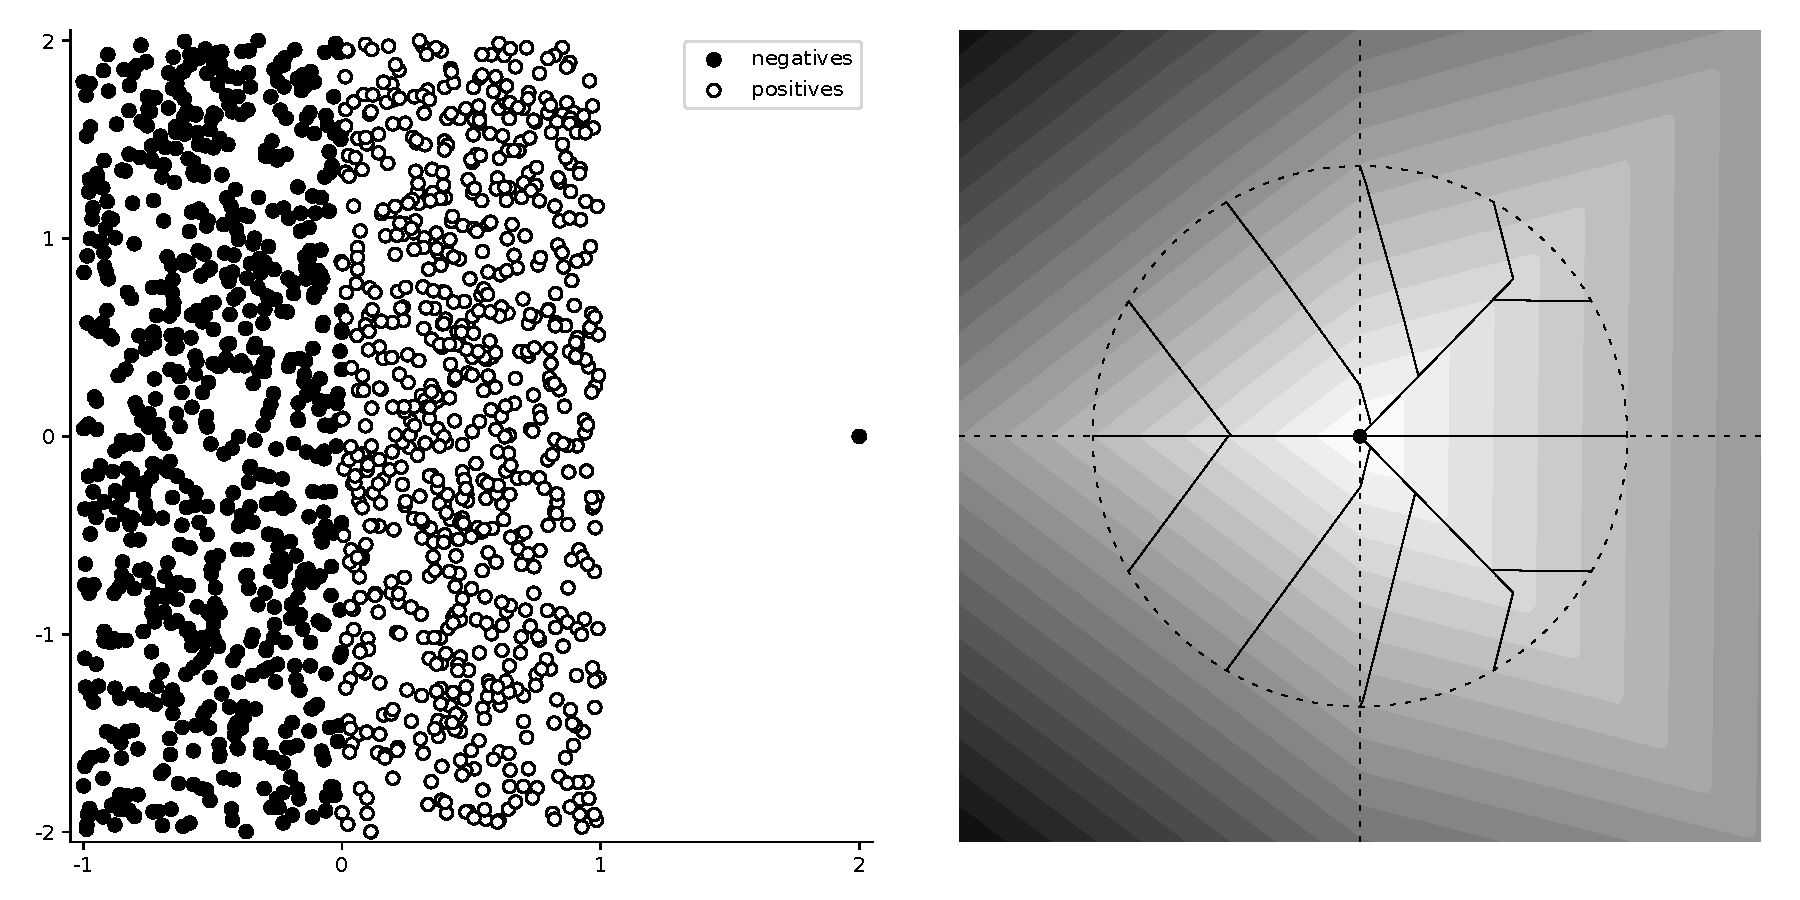
\includegraphics[width=0.7\linewidth]{data/toppush_convergence.pdf}
  \caption{Left: distribution of positive (empty circle) and negative samples (full circles) for the example from Section \ref{sec:example}. Right: contour plot for \TopPush and its convergence to the zero vector from $12$ initial points.}
  \label{fig:example}
\end{figure}

Table \ref{tab:example} shows the threshold $t$ and the objective value $f$ for two points $\bm{w}_1=(0,0)$ and $\bm{w}_2=(1,0)$. These two points are both important: $\bm{w}_1$ does not generate any separating hyperplane, while $\bm{w}_2$ generates the optimal separating hyperplane. We show the precise computation in Appendix \ref{app:example}. Since the dataset is perfectly separable by $\bm{w}_2$, we expect that $\bm{w}_2$ provides a lower objective than $\bm{w}_1$. By shading the better objective in Table~\ref{tab:example} by grey, we see that this did not happen for \TopPush and \TopMeanK.

\begin{table}[!ht]
  \caption{Comparison of formulations on the very simple problem from Section \ref{sec:example}. Two formulations have the global minimum (denoted by grey color) at $\bm{w}_1=(0,0)$ which does not generate any separating hyperplane. The optimal separating hyperplane is generated by $\bm{w}_2=(1,0)$.}
  \label{tab:example}
  \centering
  \begin{tabular}{@{}l ccccc@{}}\toprule
    & & \multicolumn{2}{c}{$\bm{w}_1=(0,0)$} & \multicolumn{2}{c}{$\bm{w}_2=(1,0)$} \\ \cmidrule(lr){3-4} \cmidrule(lr){5-6}
    Name & Label & $t$& $f$ & $t$ & $f$ \\
    \midrule
    \TopPush & \eqref{eq:problem_toppush} & $0$ & \cellcolor{gray!40}$1$ & $2$ & $2.5$ \\
    \TopPushK & \eqref{eq:problem_toppushk} & $0$ & $1$ & $\frac2k$ & \cellcolor{gray!40}$0.5+\frac2k$ \\
    \Grill & \eqref{eq:problem_grill} & $0$ & $2$ & $1-2\tau$ & \cellcolor{gray!40}$1.5+2\tau(1-\tau)$ \\
    \TopMeanK & \eqref{eq:problem_topmeank} & $0$ & \cellcolor{gray!40}$1$ & $1-\tau$ & $1.5-\tau$ \\
    \PatMat & \eqref{eq:problem_patmat}  & $\frac{1}{\beta}(1-\tau)$ & $1+\frac{1}{\beta}(1-\tau)$ & $\frac{1}{\beta}(1-\tau)$ & \cellcolor{gray!40}$0.5+\frac{1}{\beta}(1-\tau)$ \\
    \bottomrule
  \end{tabular}
\end{table}

It can be shown that $\bm{w}_1=(0,0)$ is even the global minimum for \TopPush and \TopMeanK. This raises the question of whether some tricks, such as early stopping or excluding a small ball around zero, cannot overcome this difficulty. The answer is negative as shown in Figure \ref{fig:example} (right). Here, we run \TopPush from several starting points, and it always converges to zero from one of the three possible directions; all of them far from the normal vector to the separating hyperplane.

\subsubsection{Stability and Global minimum at zero}\label{sec:w_zero}

The convexity derived in the previous section guarantees that there are no local minima. However, as we showed in the example above, the global minimum may be at $\bm{w} = \bm{0}$. This is highly undesirable since $\bm{w}$ is the normal vector to the separating hyperplane and the zero vector provides no information. In this section, we analyze when this situation happens. The first result states that if the threshold $t(\bm{w})$ is above a certain value, then zero has a better objective that $\bm{w}$. If this happens for all $\bm{w}$, then zero is the global minimum.

\begin{restatable}{theorem}{larget}\label{thm:large_t}
  Consider any of these formulations: \TopPush, \TopPushK, \TopMeanK or \tauFPL. Fix any $\bm{w}$ and denote the corresponding threshold $t(\bm{w})$. If we have
  \begin{equation*}
    t(\bm{w})\ge \frac{1}{n^+} \sum_{\bm{x}^+ \in \Xc^+} \bm{w}^\top \bm{x}^+,
  \end{equation*}
  then $f(\bm{0})\le f(\bm{w})$. Specifically, denote the scores $s^+=\bm{w}^\top \bm{x}^+$ for $\bm{x}^+\in \Xc^+$ and $s^-=\bm{w}^\top \bm{x}^-$ for $\bm{x}^-\in \Xc^-$ and the ordered variants with decreasing components of $\bm{s}^-$ by $\bm{s}_{[\cdot]}^-$. Then
  \begin{equation}\label{eq:w_zero}
    \begin{aligned}
    s_{[1]}^- \ge \frac{1}{n^+} \sum_{i=1}^{n^+} s_{i}^+
    & \implies f(\bm{0}) \le f(\bm{w}) \text{ for } \TopPush, \\
    \frac{1}{k}\sum_{i=1}^k s_{[i]}^- \ge \frac{1}{n^+} \sum_{i=1}^{n^+} s_{i}^+
    & \implies f(\bm{0})\le f(\bm{w}) \text{ for } \TopPushK, \\
    \frac{1}{n^-\tau} \sum_{i=1}^{n^-\tau} s_{[i]}^- \ge \frac{1}{n^+}\sum_{i=1}^{n^+} s_{i}^+
    & \implies f(\bm{0}) \le f(\bm{w}) \text{ for } \tauFPL. \\
    \end{aligned}
  \end{equation}
\end{restatable}

We can use this result immediately to deduce that some formulations have the global minimum at $\bm{w} = \bm{0}$. More specifically, \TopPush fails if there are outliers, and \TopMeanK fails whenever there are many positive samples.

\begin{corollary}\label{cor:toppush}
  Consider the \TopPush formulation. If the positive samples lie in the convex hull of negative samples, then $\bm{w}=\bm{0}$ is the global minimum.
\end{corollary}

\begin{corollary}\label{cor:topmean}
  Consider the \TopMeanK formulation. If $n^+\ge n\tau$, then $\bm{w}=\bm{0}$ is the global minimum.
\end{corollary}

The proof of Theorem \ref{thm:large_t} employs the fact that all formulations in the theorem statement have only false-negatives in the objective. If $\bm{w}_0=\bm{0}$, then $\bm{w}_0^\top \bm{x}=0$ for all samples $\bm{x}$, the threshold equals to $t=0$ and the objective equals to one. If the threshold is large for $\bm{w}$, many positives are below the threshold, and the false-negatives have the average surrogate value larger than one. In such a case, $\bm{w}_0=\bm{0}$ becomes the global minimum. There are two fixes to this situation:
\begin{itemize}
  \item Include false-positives to the objective. This approach is taken by \Grill and \GrillNP and necessarily results in the loss of convexity.  \item Move the threshold away from zero even when all scores $\bm{w}^\top \bm{x}$ are zero. This approach is taken by our formulations \PatMat and \PatMatNP and keeps convexity.
\end{itemize}
The next theorem shows the advantage of the second approach.

\begin{restatable}{theorem}{patmatzero}\label{thm:patmat_zero}
  Consider the \PatMat or \PatMatNP formulation with the hinge surrogate and no regularization. Assume that for some $\bm{w}$ we have
  \begin{equation}\label{eq:patmat_zero}
    \frac{1}{n^+}\sum_{\bm{x}^+ \in \Xc^+}\bm{w}^\top \bm{x}^+ > \frac{1}{n^-}\sum_{\bm{x}^- \in \Xc^-}\bm{w}^\top \bm{x}^-.
  \end{equation}
  Then there is a scaling parameter $\beta_0$ from \eqref{eq:defin_quantile0} such that $f(\bm{w})<f(\bm{0})$ for all $\beta\in(0,\beta_0)$.
\end{restatable}

These theorem shed some light on the behaviour of the formulations. Theorem \ref{thm:large_t} states that the stability of \tauFPL requires
\begin{equation}\label{eq:stability1}
  \frac{1}{n^-\tau}\sum_{i=1}^{n^-\tau}s_{[i]}^- < \frac{1}{n^+}\sum_{i=1}^{n^+} s_{i}^+,
\end{equation}
while Theorem \ref{thm:patmat_zero} states that the stability of \PatMatNP is ensured by
\begin{equation}\label{eq:stability2}
  \frac{1}{n^-}\sum_{i=1}^{n^-}s_{[i]}^- < \frac{1}{n^+}\sum_{i=1}^{n^+} s_{i}^+.
\end{equation}
The right-hand sides of \eqref{eq:stability1} and \eqref{eq:stability2} are the same, while the left-hand side of \eqref{eq:stability2} is always smaller than the left-hand side of \eqref{eq:stability1}. This implies that if \tauFPL is stable, then \PatMatNP is stable as well.

At the same time, there may be a huge difference in the stability of both formulations. Since the scores of positive samples should be above the scores of negative samples, the scores $s$ may be interpreted as performance. Then formula \eqref{eq:stability1} states that if the mean performance of a \emph{small number of the best} negative samples is larger than the average performance of \emph{all} positive samples, then \tauFPL fails. On the other hand, formula \eqref{eq:stability2} states that if the average performance of \emph{all} positive samples is better than the average performance of \emph{all} negative samples, then \PatMatNP is stable. The former may well happen as accuracy at the top is interested in a good performance of only a small number of positive samples.

\subsection{Method comparison}

We provide a summary of the obtained results in Table \ref{tab:methods}. There we give basic characterizations of the formulations such as their definition label, their source, the hyperparameters, whether the formulation is differentiable and convex, and whether it has stability problems with $\bm{w}=\bm{0}$ being the global minimum. 

\begin{table}[!ht]
  \caption{Summary of the formulations from Section \ref{sec:framework}. The table shows their definition label, the source or the source they are based on, the hyperparameters, whether the formulation is differentiable, convex and stable (in the sense of having problems with $\bm{w}=\bm{0}$).}
  \label{tab:methods}
  \centering
  \begin{tabular}{ll ccccc}\toprule
    Name & Source & Definition & Hyperpars & Convex & Differentiable & Stable \\
    \midrule
    \TopPush & \cite{Li_TopPush} & \eqref{eq:problem_toppush}& $\lambda$ & \yesmark & \nomark & \nomark\\
    \TopPushK & ours & \eqref{eq:problem_toppushk} & $\lambda$, $k$ & \yesmark & \nomark & \nomark\\ 
    \Grill & \cite{Grill_2016} & \eqref{eq:problem_grill}  & $\lambda$ & \nomark & \nomark & \yesmark\\
    \PatMat & ours & \eqref{eq:problem_patmat} & $\beta$, $\lambda$ & \yesmark & \yesmark & \yesmark\\ 
    \TopMeanK & - & \eqref{eq:problem_topmeank} & $\lambda$ & \yesmark & \nomark & \nomark\\ 
    \GrillNP & - & \eqref{eq:problem_grill_np} & $\lambda$ & \nomark & \nomark & \yesmark\\
    \PatMatNP & ours & \eqref{eq:problem_patmat_np} & $\beta$, $\lambda$ & \yesmark & \yesmark & \yesmark\\
    \tauFPL & \cite{zhang2018tau} & \eqref{eq:problem_topmeank_np} & $\lambda$ & \yesmark & \nomark & \nomark\\
    \bottomrule
  \end{tabular}
\end{table}

A similar comparison is performed in Figure \ref{fig:thresholds}. Methods in green and grey are convex, while formulations in white are non-convex. Based on Theorem \ref{thm:large_t}, four formulations in grey are vulnerable to have the global minimum at $\bm{w}=0$. This theorem states that the higher the threshold, the more vulnerable the formulation is. The full arrows depict this dependence. If it points from one formulation to another, the latter one has a smaller threshold and thus is less vulnerable to this undesired global minima. The dotted arrows indicate that this holds usually but not always, the precise formulation is provided in Appendix \ref{app:relations}. This complies with Corollaries \ref{cor:toppush} and \ref{cor:topmean} which state that \TopPush and \TopMeanK are most vulnerable. At the same time, it says that \tauFPL is the best one from the grey-coloured formulations. Finally, even though \PatMatNP has a worse approximation of the true threshold than \tauFPL due to Theorem \ref{thm:large_t}, it is more stable due to the discussion after Theorem \ref{thm:patmat_zero}.

\begin{figure}[!ht]
  \centering
  \begin{tikzpicture}[node distance=3cm]
  \node (tikz1) [bubbleB] {\TopPush};
  \node (tikz2) [bubbleB, right of=tikz1] {\TopPushK};
  \node (tikz3) [bubbleA, above right of=tikz2] {\PatMatNP};
  \node (tikz4) [bubbleB, below right of=tikz2] {\tauFPL};
  \node (tikz5) [bubbleC, below right of=tikz3] {\GrillNP};
  \draw [arrowA] (tikz1) -- (tikz2);
  \draw [arrowA] (tikz2) -- (tikz4);
  \draw [arrowA] (tikz3) -- (tikz5);
  \draw [arrowA] (tikz4) -- (tikz5);
  \draw [arrowA] (tikz3) -- (tikz4);
  %
  \node (tikz8) [bubbleC, right of=tikz5] {\Grill};
  \node (tikz6) [bubbleA, above right of=tikz8] {\PatMat};
  \node (tikz7) [bubbleB, below right of=tikz8] {\TopMeanK};
  \draw [arrowA] (tikz6) -- (tikz8);
  \draw [arrowA] (tikz7) -- (tikz8);
  \draw [arrowA] (tikz6) -- (tikz7);
  %
  \draw [arrowB] (tikz6) -- (tikz3);
  \draw [arrowB] (tikz7) -- (tikz4);
  \draw [arrowB] (tikz8) -- (tikz5);
  %
  \node (comm2) [bubbleB, minimum height=3mm, node distance=4.1cm, left of=tikz3] {\phantom{not }convex, not stable};
  \node (comm1) [bubbleA, minimum height=3mm, node distance=6.1mm, above of=comm2] {\phantom{not }convex, \phantom{not }stable};
  \node (comm3) [bubbleC, minimum height=3mm, node distance=6.1mm, below of=comm2] {not convex, \phantom{not }stable};
  \end{tikzpicture}
  \caption{Summary of the formulations from Section \ref{sec:framework}. Methods in green and grey are convex, while formulations in white are non-convex. Methods in grey are vulnerable to have the global minimum at $\bm{w}=0$. Full (dotted) arrow pointing from one formulation to another show that the latter formulation has always (usually) smaller threshold.}
  \label{fig:thresholds}
\end{figure}

\section{Convergence of stochastic gradient descent}\label{sec:convergence}

The previous section analyzed the formulations from Section \ref{sec:framework} but did not consider any optimization algorithms. In this section, we show a basic version of the stochastic gradient descent and then show its convergent version. Since due to considering the threshold, gradient computed on a minibatch is a biased estimate of the true gradient, we need to use variance reduction techniques, and the proof is rather complex.

\subsection{Stochastic gradient descent: Basic}

Many optimization algorithms for solving the formulations from Section \ref{sec:framework} use primal-dual or purely dual formulations. \cite{Eban_2017} introduced dual variables and used alternating optimization to the resulting min-max problem.  \cite{Li_TopPush} and \cite{zhang2018tau} dualized the problem and solved it with the steepest gradient ascent. \cite{macha2020nonlinear} followed the same path but added kernels to handle non-linearity. We follow the ideas of \cite{mackey2018constrained} and \cite{adam2019machine} and solve the problems directly in their primal formulations. Therefore, even though we use the same formulation for \TopPush as \cite{Li_TopPush} or for \tauFPL as \cite{zhang2018tau}, our solution process is different. However, due to convexity, both algorithms should converge to the same point.

The decision variables in \eqref{eq:problem2} are the normal vector of the separating hyperplane $\bm{w}$ and the threshold $t$. To apply an efficient optimization method, we need to compute gradients. The simplest idea \cite{Grill_2016} is to compute the gradient only with respect to $\bm{w}$ and then recompute $t$. A more sophisticated way is based on the chain rule. For each $\bm{w}$, the threshold $t$ can be computed uniquely. We stress this dependence by writing $t(\bm{w})$ instead of $t$. By doing so, we effectively remove the threshold $t$ from the decision variables and $\bm{w}$ remains the only decision variable. Note that the convexity is preserved. Then we can compute the derivative via the chain rule
\begin{equation}\label{eq:derivatives}
  \begin{aligned}
  f(\bm{w}) & = \frac{1}{n^+}\sum_{\bm{x} \in \Xc^+} l(t(\bm{w}) - \bm{w}^\top \bm{x}) + \frac{\lambda}{2}\norm{\bm{w}}^2, \\
  \nabla f(\bm{w}) & = \frac{1}{n^+}\sum_{\bm{x} \in \Xc^+} l'(t(\bm{w}) - \bm{w}^\top \bm{x})(\nabla t(\bm{w}) - \bm{x}) + \lambda \bm{w}.
  \end{aligned}
\end{equation}
The only remaining part is the computation of $\nabla t(\bm{w})$. It is simple for $\nabla t_1(\bm{w})$ and $\nabla t_2(\bm{w})$ and Theorem \ref{thm:derivative} shows the computation for $\nabla t_3(\bm{w})$. Appendix \ref{app:threshold} provides an efficient computation method for $t_3(\bm{w})$.

Having derivative \eqref{eq:derivatives}, deriving the stochastic gradient is simple. It partitions the dataset into minibatches and provides an update of the weights $\bm{w}$ based only on a minibatch, namely by replacing the mean over the whole dataset in \eqref{eq:derivatives} by a mean over the minibatch.

\subsection{Stochastic gradient descent: Convergent for \PatMat and \PatMatNP}

For the convergence proof, we need differentiability which is due to Theorem \ref{thm:derivative} possessed only by \PatMat and \PatMatNP. Therefore, we consider only these two formulations and for simplicity, show it only for \PatMat. We apply a variance reduction technique based on delayed values similar to SAG \cite{schmidt2017minimizing}. 

At iteration $k$ we have the decision variable $\bm{w}^k$ and the active minibatch $I^k$. First, we update the score vector $\bm{s}^k$ only on the active minibatch by setting
\begin{equation}\label{eq:defin_z}
  s_i^k = \begin{cases} \bm{x}_i^\top \bm{w}^k &\text{for all }i\in I^k,\\ s_i^{k-1} &\text{for all }i\notin I^k.\end{cases} 
\end{equation}
We keep scores from previous minibatches intact. We use Appendix \ref{app:threshold} to compute the surrogate quantile $t^k$ as the unique solution of
\begin{equation}\label{eq:update_t}
  \sum_{i \in X}l(\beta(s_i^k - t^k)) = n\tau.
\end{equation}
This is an approximation of the surrogate quantile $t(\bm{w}^k)$ from \eqref{eq:defin_quantile0}. The only difference from the true value $t(\bm{w}^k)$ is that we use delayed scores. Then we introduce artificial variable
\begin{equation}\label{eq:update_a}
  \begin{aligned}
    \bm{a}^k &= \sum_{i\in I^k}l'(\beta(s_i^k - t^k))\bm{x}_i.
  \end{aligned}
\end{equation}
Finally, we approximate the derivative $\nabla f(\bm{w}^k)$ from \eqref{eq:derivatives} by
\begin{equation}\label{eq:update_g}
  g(\bm{w}^k) = \frac{1}{n^k_+}\sum_{i\in I^k_+}l'(t^k - s_i^k)(\nabla t^k - \bm{x}_i),
\end{equation}
where $\nabla t^k$ is an approximation of $\nabla t(\bm{w}^k)$ from Theorem \ref{thm:derivative} defined by
\begin{equation}\label{eq:update_nablat}
  \nabla t^k = \frac{\bm{a}^k + \bm{a}^{k-1} + \dots + \bm{a}^{k - m + 1}}{\sum_{i \in X} l'(\beta(s_i^k - t^k))}.
\end{equation}
A perhaps more straightforward possibility would be to consider only $\bm{a}^k$ in the numerator of \eqref{eq:update_nablat}. However, choice \eqref{eq:update_nablat} enables us to prove the convergence and it adds stability to the algorithm for small minibatches.

The whole procedure does not perform any vector operations outside of the current minibatch~$I^k$. We summarize it in Algorithm \ref{alg:sgd}. Note that a proper initialization for the first $m$ iterations is needed. We finish the theoretical part by the convergence proof.

\begin{algorithm}[!ht]
  \begin{algorithmic}[1]
    \Require Dataset $X$, Minibatches $I^1,\dots,I^m$, Stepsize $\alpha^k$
    \State Initialize weights $\bm{w}^0$
    \For{$k = 0,1,\dots$}
    \State Select a minibatch $I^k$
    \State Compute $s_i^k$ for all $i\in I^k$ according to \eqref{eq:defin_z}
    \State Compute $t^k$ according to \eqref{eq:update_t}
    \State Compute $\bm{a}^k$ according to \eqref{eq:update_a}
    \State Compute $\nabla t^k$ according to \eqref{eq:update_nablat}
    \State Compute $g(\bm{w}^k)$ according to \eqref{eq:update_g}
    \State Set $\bm{w}^{k+1}\gets \bm{w}^k - \alpha^k g(\bm{w}^k)$
    \EndFor
  \end{algorithmic}
  \caption{Stochastic gradient descent for maximizing accuracy at the top}
  \label{alg:sgd}
\end{algorithm}

\begin{restatable}{theorem}{sgd}\label{thm:sgd}
  Consider the \PatMat or \PatMatNP formulation, stepsizes $\alpha^k = \frac{\alpha^0}{k+1}$ and piecewise disjoint minibatches $I^1,\dots,I^m$ which cycle periodically $I^{k+m}=I^k$. If $l$ is the smoothened (Huberized) hinge function, then Algorithm \ref{alg:sgd} converges to the global minimum of \eqref{eq:problem_patmat}.  
\end{restatable}

\section{Numerical experiments}\label{sec:num1}

In this section, we present numerical results.

\subsection{Implementational details and Hyperparameter choice}

We recall that all methods fall into the framework of either \eqref{eq:problem1} or \eqref{eq:problem2}. Since the threshold $t$ depends on the weights $\bm{w}$, we can consider the decision variable to be only $\bm{w}$. Then to apply a method, we implemented the following iterative procedure. At iteration $j$, we have the weights $\bm{w}^j$ to which we compute the threshold $t^j=t(\bm{w}^j)$. Then according to \eqref{eq:derivatives}, we compute the gradient of the objective and apply the ADAM descent scheme \cite{kingma2014adam}. All methods were run for $10000$ iterations using the stochastic gradient descent. The minibatch size was $512$ except for the Ionosphere and Spambase datasets where the full gradient was used. All methods used the hinge surrogate \eqref{eq:defin_surrogate}. The initial point is generated randomly.

We run the methods for the following hyperparameters
\begin{equation}\label{eq:beta1}
  \begin{aligned}
    \beta   & \in  \{0.0001,\ 0.001,\ 0.01,\ 0.1,\ 1,\ 10\}, \\
    \lambda & \in \{0,\ 0.00001,\ 0.0001,\ 0.001,\ 0.01,\ 0.1\}, \\
    k       & \in \{1, 3, 5, 10, 15, 20\}.
  \end{aligned}
\end{equation}
For \TopPushK, \PatMat and \PatMatNP we fixed $\lambda=0.001$ to have six hyperparameters for all methods. For all datasets, we choose the hyperparameter which minimized the criterion on the validation set. The results are computed on the testing set which was not used during training the methods.

\TopPush and \tauFPL were originally implemented in the dual. However, to allow for the same framework and the stochastic gradient descent, we implemented it in the primal. These two approaches are equivalent.

\subsection{Dataset description and Performance criteria}\label{sec:datasets}

For the numerical results, we considered 10 datasets summarized in Table \ref{tab:counts}. They can be downloaded from the UCI repository. Ionosphere \cite{ionosphere} and Spambase are small, Hepmass \cite{hepmass} contains a large number of samples while Gisette \cite{gisette} contains a large number of features. We also considered six visual recognition datasets: MNIST, FashionMNIST, CIFAR10, CIFAR20, CIFAR100 and SVHN2. MNIST and FashionMNIST are grayscale datasets of digits and fashion items, respectively. CIFAR100 is a dataset of coloured images of items grouped into 100 classes. CIFAR10 and CIFAR20 merge these classes into 10 and 20 superclasses, respectively. SVHN2 contains coloured images of house numbers. As Table \ref{tab:counts} shows, these datasets are imbalanced.

Each of the visual recognition datasets was converted into ten binary datasets by considering one of the classes $\{0,\dots,9\}$ as the positive class and the rest as the negative class. The experiments were repeated ten times for each dataset from different seeds, which influenced the starting point and minibatch creation. We use tpr@fpr as the evaluation criterion. This describes the true-positive rate at a prescribed true-negative rate, usually of $1\%$ or $5\%$. For the linear classifier $\bm{w}^\top \bm{x} - t$, it selects the threshold $t$ so that the desired true-negative rate is satisfied and then computes the true-positive rate for this threshold.

\begin{table}[!ht]
  \caption{Structure of the used datasets. The training, validation and testing sets show the number of features $m$, samples $n$ and the fraction of positive samples $\frac{n^+}{n}$.}
  \label{tab:counts}
  \centering
  \begin{tabular}{@{}lllllllll@{}}
    \toprule
    &  & \multicolumn{2}{c}{Training} & \multicolumn{2}{c}{Validation} & \multicolumn{2}{c}{Testing} \\ \cmidrule(lr){3-4} \cmidrule(lr){5-6} \cmidrule(l){7-8} 
    & $m$ & $n$ & $\frac{n^+}{n}$ & $n$ & $\frac{n^+}{n}$ & $n$ & $\frac{n^+}{n}$ \\ \midrule
    Ionosphere
      & $34$
      & $175$ & $36.0\%$ & $88$ & $36.4\%$ & $88$ & $35.2\%$ \\
    Spambase
      & $57$
      & $2300$ & $39.4\%$ & $1150$ & $39.4\%$ & $1151$ & $39.4\%$ \\
    Gisette
      & $5000$
      & $1000$ & $50.0\%$ & $1500$ & $50.0\%$ & $500$ & $50.0\%$ \\
    Hepmass
      & $28$
      & $5250000$ & $50.0\%$ & $1750000$ & $50.0\%$ & $3500000$ & $50.0\%$ \\
    MNIST
      & $28 \times 28 \times 1$
      & $44999$ & $11.2\%$ & $15001$ & $11.2\%$ & $10000$ & $11.4\%$ \\
    FashionMNIST
      & $28 \times 28\times 1$
      & $45000$ & $10.0\%$ & $15000$ & $10.0\%$ & $10000$ & $10.0\%$ \\
    CIFAR10
      & $32\times 32\times 3$
      & $37500$ & $10.0\%$ & $12500$ & $10.0\%$ & $10000$ & $10.0\%$ \\
    CIFAR20
      & $32 \times 32\times 3$
      & $37500$ & $5.0\%$ & $12500$ & $5.0\%$ & $10000$ & $5.0\%$ \\
    CIFAR100
      & $32 \times 32\times 3$
      & $37500$ & $1.0\%$ & $12500$ & $1.0\%$ & $10000$ & $1.0\%$ \\
    SVHN2
      & $32 \times 32\times 3$
      & $54944$ & $18.9\%$ & $18313$ & $18.9\%$ & $26032$ & $19.6\%$ \\
    \bottomrule
  \end{tabular}
\end{table}

\subsection{Numerical results}

Figure \ref{fig:ptau} presents the standard ROC (receiver operating characteristic) curves on selected datasets. Since all methods from this paper are supposed to work at low false-positive rates, the $x$ axis is logarithmic. Both figures depict averages over ten runs with different seeds. The left column depicts CIFAR100 while the right one Hepmass. These are the two more complicated datasets. We selected four representative methods: \PatMat and \PatMatNP as our methods and \TopPush and \tauFPL as state-of-the-art methods. Even though all methods work well, \PatMatNP seems to outperform the remaining methods on most levels of false-positive rate.

\begin{figure}[!ht]
  \centering
  \begin{tikzpicture}
    \pgfplotsset{
      xlabel={False negative rate},
      ylabel={True positive rate},
      xmin = 0.0001,
      xmax = 1,
      xmode = log,
      ymin = -0.05,
      ymax = 1.05,
      ytick = {0,0.2,0.4,0.6,0.8,1},
      grid=major,
      grid style={dashed, gray!50},
      axis x line*=bottom,
    }
    \begin{groupplot}[
        group style = {group size = 2 by 1, horizontal sep = 20pt},
      ]
      \nextgroupplot[
        legend to name={Leg},
        legend style={legend columns=4, column sep = 10pt},
      ]
      \addplot [LinePatMatNP] table[x index=12, y index=13] {\DataCIFAR};
      \addlegendentry{\PatMatNP}
      \addplot [LineTopPush] table[x index=20, y index=21] {\DataCIFAR};
      \addlegendentry{\TopPush}
      \addplot [LinePatMat] table[x index=8, y index=9] {\DataCIFAR};
      \addlegendentry{\PatMat}
      \addplot [LinetauFPL] table[x index=24, y index=25] {\DataCIFAR};
      \addlegendentry{\tauFPL}

      \nextgroupplot[ylabel = {}, yticklabels={}]
      \addplot [LinePatMatNP] table[x index=12, y index=13] {\DataHEPMASS};
      \addplot [LineTopPush] table[x index=20, y index=21] {\DataHEPMASS};
      \addplot [LinePatMat] table[x index=8, y index=9] {\DataHEPMASS};
      \addplot [LinetauFPL] table[x index=24, y index=25] {\DataHEPMASS};
    \end{groupplot}
    \path (group c1r1.north east) -- node[above]{\ref{Leg}} (group c2r1.north west);
  \end{tikzpicture}
  \caption{ROC curves (with logarithmic $x$ axis) on CIFAR100 (left) and Hepmass (right).}
  \label{fig:ptau}
\end{figure}

While Figure \ref{fig:ptau} gave a glimpse of the behaviour of methods, Figures \ref{fig:cd1} and~\ref{fig:cd2} provide a statistically more sound comparison. It employs the Nemenyi post hoc test for the Friedman test recommended in \cite{demvsar2006statistical}. This test compares if the mean ranks of multiple methods are significantly different.

We consider 14 methods (we count different values of $\tau$ as different methods) as depicted in this table. For each dataset mentioned in Section \ref{sec:datasets} and each method, we evaluated the fpr@tpr metric and ranked all methods. Rank 1 refers to the best performance for given criteria, while rank 14 is the worst. The $x$-axis shows the average rank over all datasets. The Nemenyi test computes the critical difference. If two methods are within their critical difference, their performance is not deemed to be significantly different. Black wide horizontal lines group such methods.

\begin{figure}[!ht]
    \centering
    \resizebox{\linewidth}{!}{
  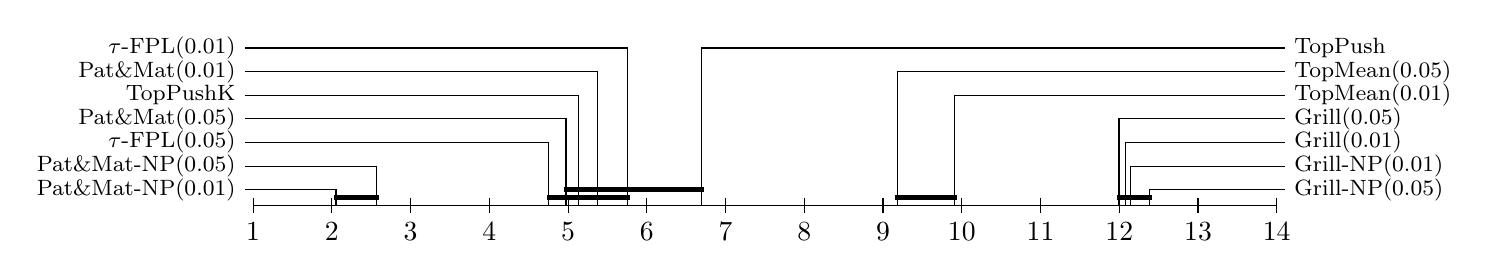
\begin{tikzpicture}[scale = 1.0]
    \draw (1.0,0) -- (14.0,0);
    \foreach \x in {1,...,14} \draw (\x,0.10) -- (\x,-0.10) node[anchor=north]{$\x$};
    \draw (2.051948051948052,0) -- (2.051948051948052,0.19999999999999998) -- (0.9, 0.19999999999999998) node[anchor=east] {\footnotesize Pat\&Mat-NP(0.01)};
    \draw (2.564935064935065,0) -- (2.564935064935065,0.5) -- (0.9, 0.5) node[anchor=east] {\footnotesize Pat\&Mat-NP(0.05)};
    \draw (4.7564935064935066,0) -- (4.7564935064935066,0.7999999999999999) -- (0.9, 0.7999999999999999) node[anchor=east] {\footnotesize $\tau$-FPL(0.05)};
    \draw (4.974025974025974,0) -- (4.974025974025974,1.0999999999999999) -- (0.9, 1.0999999999999999) node[anchor=east] {\footnotesize Pat\&Mat(0.05)};
    \draw (5.136363636363637,0) -- (5.136363636363637,1.4) -- (0.9, 1.4) node[anchor=east] {\footnotesize TopPushK};
    \draw (5.37012987012987,0) -- (5.37012987012987,1.6999999999999997) -- (0.9, 1.6999999999999997) node[anchor=east] {\footnotesize Pat\&Mat(0.01)};
    \draw (5.753246753246753,0) -- (5.753246753246753,2.0) -- (0.9, 2.0) node[anchor=east] {\footnotesize $\tau$-FPL(0.01)};
    \draw (6.694805194805195,0) -- (6.694805194805195,1.9999999999999998) -- (14.1, 1.9999999999999998) node[anchor=west] {\footnotesize TopPush};
    \draw (9.181818181818182,0) -- (9.181818181818182,1.7) -- (14.1, 1.7) node[anchor=west] {\footnotesize TopMean(0.05)};
    \draw (9.905844155844155,0) -- (9.905844155844155,1.4) -- (14.1, 1.4) node[anchor=west] {\footnotesize TopMean(0.01)};
    \draw (11.996753246753247,0) -- (11.996753246753247,1.0999999999999999) -- (14.1, 1.0999999999999999) node[anchor=west] {\footnotesize Grill(0.05)};
    \draw (12.084415584415584,0) -- (12.084415584415584,0.8) -- (14.1, 0.8) node[anchor=west] {\footnotesize Grill(0.01)};
    \draw (12.146103896103897,0) -- (12.146103896103897,0.5) -- (14.1, 0.5) node[anchor=west] {\footnotesize Grill-NP(0.01)};
    \draw (12.383116883116884,0) -- (12.383116883116884,0.2) -- (14.1, 0.2) node[anchor=west] {\footnotesize Grill-NP(0.05)};
    \draw[line width=0.06cm,color=black,draw opacity=1.0] (2.021948051948052,0.1) -- (2.594935064935065,0.1);
    \draw[line width=0.06cm,color=black,draw opacity=1.0] (4.726493506493506,0.1) -- (5.783246753246753,0.1);
    \draw[line width=0.06cm,color=black,draw opacity=1.0] (4.9440259740259735,0.2) -- (6.724805194805195,0.2);
    \draw[line width=0.06cm,color=black,draw opacity=1.0] (9.151818181818182,0.1) -- (9.935844155844155,0.1);
    \draw[line width=0.06cm,color=black,draw opacity=1.0] (11.966753246753248,0.1) -- (12.413116883116883,0.1);
  \end{tikzpicture}
}

    \caption{Critical difference (CD) diagrams (level of importance 0.05) of the Nemenyi post hoc test for the Friedman test. Each diagram shows the mean rank of each method, with rank 1 being the best. Black wide horizontal lines group together methods with the mean ranks that are not significantly different. The critical difference diagrams were computed for mean rank averages over all datasets of the tpr@fpr ($\tau=0.01$) metric.}
    \label{fig:cd1}
\end{figure}

\begin{figure}[!ht]
    \centering
    \resizebox{\linewidth}{!}{
  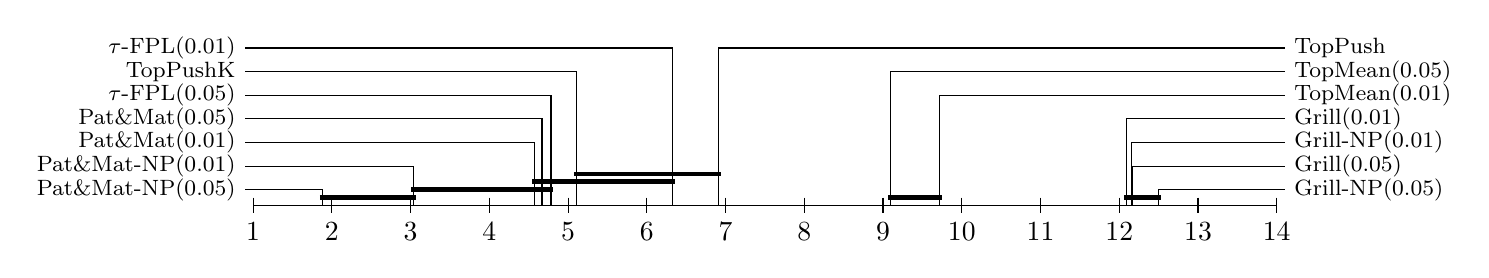
\begin{tikzpicture}[scale = 1.0]
    \draw (1.0,0) -- (14.0,0);
    \foreach \x in {1,...,14} \draw (\x,0.10) -- (\x,-0.10) node[anchor=north]{$\x$};   \draw (1.8766233766233766,0) -- (1.8766233766233766,0.19999999999999998) -- (0.9, 0.19999999999999998) node[anchor=east] {\footnotesize Pat\&Mat-NP(0.05)};
    \draw (3.0357142857142856,0) -- (3.0357142857142856,0.5) -- (0.9, 0.5) node[anchor=east] {\footnotesize Pat\&Mat-NP(0.01)};
    \draw (4.577922077922078,0) -- (4.577922077922078,0.7999999999999999) -- (0.9, 0.7999999999999999) node[anchor=east] {\footnotesize Pat\&Mat(0.01)};
    \draw (4.6688311688311686,0) -- (4.6688311688311686,1.0999999999999999) -- (0.9, 1.0999999999999999) node[anchor=east] {\footnotesize Pat\&Mat(0.05)};
    \draw (4.782467532467533,0) -- (4.782467532467533,1.4) -- (0.9, 1.4) node[anchor=east] {\footnotesize $\tau$-FPL(0.05)};
    \draw (5.103896103896104,0) -- (5.103896103896104,1.6999999999999997) -- (0.9, 1.6999999999999997) node[anchor=east] {\footnotesize TopPushK};
    \draw (6.327922077922078,0) -- (6.327922077922078,2.0) -- (0.9, 2.0) node[anchor=east] {\footnotesize $\tau$-FPL(0.01)};
    \draw (6.9058441558441555,0) -- (6.9058441558441555,1.9999999999999998) -- (14.1, 1.9999999999999998) node[anchor=west] {\footnotesize TopPush};
    \draw (9.097402597402597,0) -- (9.097402597402597,1.7) -- (14.1, 1.7) node[anchor=west] {\footnotesize TopMean(0.05)};
    \draw (9.714285714285714,0) -- (9.714285714285714,1.4) -- (14.1, 1.4) node[anchor=west] {\footnotesize TopMean(0.01)};
    \draw (12.090909090909092,0) -- (12.090909090909092,1.0999999999999999) -- (14.1, 1.0999999999999999) node[anchor=west] {\footnotesize Grill(0.01)};
    \draw (12.152597402597403,0) -- (12.152597402597403,0.8) -- (14.1, 0.8) node[anchor=west] {\footnotesize Grill-NP(0.01)};
    \draw (12.162337662337663,0) -- (12.162337662337663,0.5) -- (14.1, 0.5) node[anchor=west] {\footnotesize Grill(0.05)};
    \draw (12.503246753246753,0) -- (12.503246753246753,0.2) -- (14.1, 0.2) node[anchor=west] {\footnotesize Grill-NP(0.05)};
    \draw[line width=0.06cm,color=black,draw opacity=1.0] (1.8466233766233766,0.1) -- (3.0657142857142854,0.1);
    \draw[line width=0.06cm,color=black,draw opacity=1.0] (3.005714285714286,0.2) -- (4.812467532467533,0.2);
    \draw[line width=0.06cm,color=black,draw opacity=1.0] (4.5479220779220775,0.30000000000000004) -- (6.357922077922078,0.30000000000000004);
    \draw[line width=0.06cm,color=black,draw opacity=1.0] (5.073896103896104,0.4) -- (6.935844155844156,0.4);
    \draw[line width=0.06cm,color=black,draw opacity=1.0] (9.067402597402598,0.1) -- (9.744285714285713,0.1);
    \draw[line width=0.06cm,color=black,draw opacity=1.0] (12.060909090909092,0.1) -- (12.533246753246752,0.1);
  \end{tikzpicture}
}

    \caption{Critical difference (CD) diagrams (level of importance 0.05) of the Nemenyi post hoc test for the Friedman test. Each diagram shows the mean rank of each method, with rank 1 being the best. Black wide horizontal lines group together methods with the mean ranks that are not significantly different. The critical difference diagrams were computed for mean rank averages over all datasets of the tpr@fpr ($\tau=0.05$) metric.}
    \label{fig:cd2}
\end{figure}

From this figure and table, we make several observations:
\begin{itemize}
  \item \TopPushK (rank 5.1) provides a slight improvement over \TopPush (rank 6.7) even though this improvement is not statistically significant as both methods are connected by the black line in both Figures \ref{fig:cd1} and \ref{fig:cd2}.
  \item Neither \Grill (ranks 12.0 and 12.1) nor \GrillNP (ranks 12.1 and 12.4) perform well. We believe this happened due to the lack of convexity as indicated in Theorem \ref{thm:convex} and the discussion after that.
  \item \TopMeanK (ranks 9.2 and 9.9) does not perform well either. Since the thresholds $\tau$ are small, then $\bm{w}=0$ is the global minimum as proved in Corollary \ref{cor:topmean}.
  \item \PatMatNP (rank 2.1 and 2.6) seems to outperform other methods.
  \item \PatMat (ranks 5.0 and 5.4), \tauFPL (ranks 4.8 and 5.8) and \TopPushK (rank 5.1) perform similarly. Since they are connected, there is no statistical difference between their behaviours.
  \item \PatMatNP at level $0.01$ (rank 2.1) outperforms \PatMatNP at level $0.05$ (rank 2.6) for $\tau=0.01$. \PatMatNP at level $0.05$ (rank 1.9 in Figure \ref{fig:cd2}) outperforms \PatMatNP at level $0.01$ (rank 3.0 in Figure \ref{fig:cd2}) for $\tau=0.05$. This should be because these methods are optimized for the corresponding threshold. For $\tauFPL$ we observed this behaviour for Figure \ref{fig:cd2} but not for Figure \ref{fig:cd1}.
\end{itemize}

Figure \ref{fig:wilcoxon} provides a similar comparison. Both axes are sorted from the best (left) to the worst (right) average ranks. The numbers in the graph show the $p$-value for the pairwise Wilcoxon signed-rank test, where the null hypothesis is that the mean tpr@fpr of both methods is the same. Even though Figure \ref{fig:cd1} employs a comparison of mean ranks and Figure \ref{fig:wilcoxon} a pairwise comparison of fpr@tpr, the results are almost similar. Methods grouped by the black line in the former figure usually show a large $p$-value in the latter figure.

\begin{figure}[!ht]
    \centering
    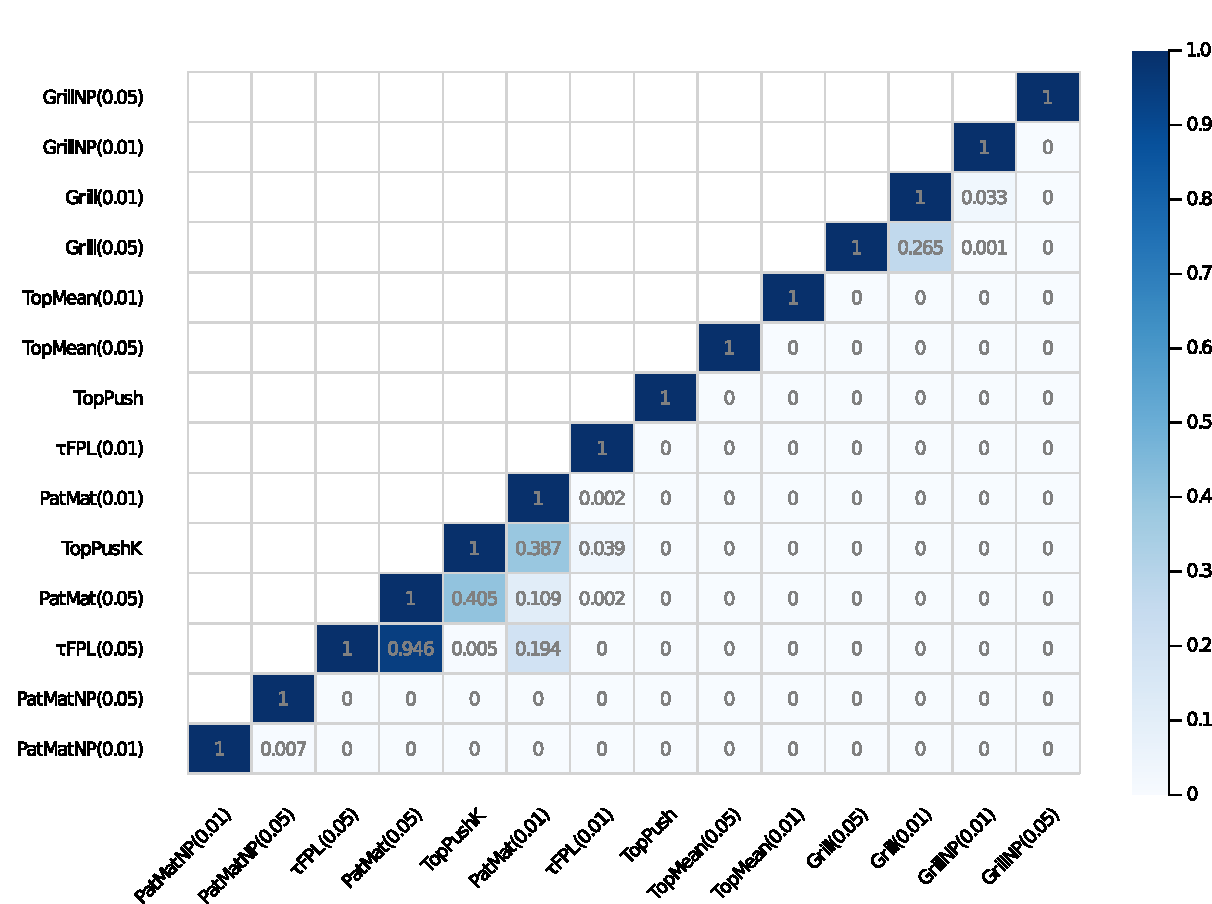
\includegraphics[width = \linewidth]{data/wilcoxon_fpr_1.pdf}
    \caption{The $p$-value for the parwise Wilcoxon signed-rank test, where the null hypothesis is that the mean tpr@fpr(0.01) of both methods is the same. The methods are sorted by mean rank (left = better).}
    \label{fig:wilcoxon}
\end{figure}

Table \ref{tab:fails} investigates the impact of $\bm{w}=0$ as a potential global minimum. Each method was optimized for six different values of hyperparameters. The table depicts the condition under which the final value has a lower objective than $\bm{w}=0$. Thus, \yesmark\ means that it is always better while \nomark\ means that the algorithm made no progress from the starting point $\bm{w} =0$. The latter case implies that $\bm{w}=0$ seems to be the global minimum. We make the following observations:
\begin{itemize}
  \item \PatMat and \PatMatNP are the only methods which succeeded at every dataset for some hyperparameter. Moreover, for each dataset, there was some $\beta_0$ such that these methods were successful if and only if $\beta\in(0,\beta_0)$. This is in agreement with Theorem~\ref{thm:patmat_zero}.
  \item \TopMeanK fails everywhere which agrees with Corollary \ref{cor:topmean}.
  \item Figure \ref{fig:thresholds} states that the methods from Section \ref{sec:obj2} has a higher threshold than their Neyman-Pearson variants from Section \ref{sec:obj3}. This is documented in the table as the latter have a higher number of successes.
\end{itemize}

\begin{table}[!ht]
  \caption{Necessary hyperparameter choice for the solution to have a better objective than zero. \yesmark\ means that the solution was better than zero for all hyperparameters while \nomark\ means that it was worse for all hyperparameters.}
  \label{tab:fails}
  \centering
  \begin{tabular}{@{}lllll@{}}
    \toprule
    & Ionosphere & Hepmass & FashionMNIST & CIFAR100 \\
    \midrule
    \TopPush
      & \yesmark & \nomark & \yesmark & \nomark \\
    \TopPushK
      & \yesmark & \nomark & \yesmark & \nomark \\
    \Grill$\tau=0.01$
      & \nomark & \nomark & \nomark & \nomark \\
    \phantom{\Grill}$\tau=0.05$
      & \nomark &\nomark & \nomark & \nomark \\
    \PatMat$\tau=0.01$
      & \yesmark & \good{\boldmath$\beta\le 0.1$} & \good{\boldmath$\beta\le 1$} & \good{\boldmath$\beta\le 1$} \\
    \phantom{\PatMat}$\tau=0.05$
      & \yesmark & \good{\boldmath$\beta\le 1$} & \yesmark & \yesmark \\
    \TopMeanK$\tau=0.01$
      & \nomark & \nomark & \nomark & \nomark \\
    \phantom{\TopMeanK}$\tau=0.05$
      & \nomark & \nomark & \nomark & \nomark \\
    \GrillNP$\tau=0.01$
      & \nomark & \nomark & \nomark & \nomark \\
    \phantom{\GrillNP}$\tau=0.05$
      & \nomark & \nomark & \nomark & \nomark \\
    \PatMatNP$\tau=0.01$
      & \yesmark & \good{\boldmath$\beta\le 1$} & \yesmark & \good{\boldmath$\beta\le 1$} \\
    \phantom{\PatMatNP}$\tau=0.05$
      & \yesmark & \yesmark & \yesmark & \good{\boldmath$\beta\le 1$} \\
    \tauFPL$\tau=0.01$
      & \yesmark & \nomark & \yesmark & \nomark \\
    \phantom{\tauFPL}$\tau=0.05$
      & \yesmark & \yesmark & \yesmark & \good{\boldmath$\lambda\le 0.001$} \\
    \bottomrule
  \end{tabular}
\end{table}

\section{Conclusion}

In this paper, we achieved the following results:
\begin{itemize}
  \item We presented a unified framework for the three criteria from Section \ref{sec:framework}. These criteria include ranking, accuracy at the top and hypothesis testing.
  \item We showed that several known methods (\TopPush, \Grill, \tauFPL) fall into our framework and derived some completely new methods (\PatMat, \PatMatNP).
  \item We performed a theoretical analysis of the methods. We showed that known methods suffer from certain disadvantages. While \TopPush and \tauFPL are sensitive to outliers, \Grill is non-convex. We proved the global convergence of the stochastic gradient descent for \PatMat and \PatMatNP.
  \item We performed a numerical comparison and we showed a good performance of our method \PatMatNP.
\end{itemize}
\chapter{Non-linear Classification at the Top}

\section{Introduction}
    
The aim of classical linear binary classification is to separate positive and negative samples by a linear hyperplane. In many applications, it is desirable to separate only a certain number of samples. In such a case, the goal is not to maximize the performance on all samples but only the performance on the required samples with the highest relevance. Such classifiers have many applications. For example, in information retrieval systems, only the most relevant documents should be returned for a given query. Furthermore, they are useful in domains, where a large number of samples needs to be quickly screened and only a small subset of samples needs to be selected for further evaluation.

These problems can be generally written as pushing the positive samples above some decision threshold. The methods differ in the definition of the decision threshold. In our previous work~\cite{adam2019patmat}, we introduced a general framework that unifies these methods. We showed that several problem classes, which were considered as separate problems so far, fit into the framework. As the most relevant we mention the following methods:
\begin{itemize}
  \item \emph{Ranking problems} focuses on ranking the positive samples higher than the negative ones. Many methods, such as \emph{RankBoost}~\cite{freund2003efficient}, \emph{Infinite Push}~\cite{agarwal2011infinite} or \emph{$p$-norm push}~\cite{rudin2009pnorm} employ a pairwise comparison of samples, which makes them infeasible for larger datasets. This was alleviated in \TopPush~\cite{li2014top} where the authors considered the limit~$p \rightarrow \infty$. Since the $l_{\infty}$ norm from \TopPush is equal to the maximum, the decision threshold from our framework equals to the maximum of scores of negative samples. This was generalized into \TopPushK~\cite{adam2019patmat} by considering the threshold to be the mean of~$K$ largest scores of negative samples.

  \item \AccatTop~\cite{boyd2012accuracy} focuses on maximizing the number of positive samples above the top $\tau$-quantile of scores. There are many methods on how to solve accuracy at the top. In~\cite{boyd2012accuracy}, the authors assume that the top quantile is one of the samples, construct~$n$ unconstrained optimization problems with fixed thresholds, solve them and select the best solution. This method is computationally expensive. In~\cite{grill2016learning} the authors propose a fast projected gradient descent method. In our previous paper, we proposed a convex approximation of the accuracy at the top called \PatMat. This method is reasonably fast and guaranteed the existence of global optimum.
\end{itemize}

The deficiency of methods from this framework is that they usually cover only linear classifiers. However, as many problems are not linearly separable, nonlinear classifiers are needed. In this work, we show how to extend our framework into nonlinear classification problems. To do so, we use the fact that our framework is similar to the primal formulation of support vector machines~\cite{cortes1995support}. The classical way to incorporate nonlinearity into SVM is to derive the dual formulation~\cite{boyd2004convex} and to employ the kernels method~\cite{scholkopf2001learning}. In this work, we follow this approach, derive dual formulations for the considered problems and add nonlinear kernels to them. Moreover, as dual problems are generally expensive to solve, we derive a quick method to solve them. This is a modification of the coordinate-wise dual ascent from~\cite{hsieh2008dual}. For a review of other approaches see \cite{batmaz2019review,werner2019review}.

The paper is organized as follows: In Section~\ref{sec:Derivation of dual problems} we recall the unified framework derived in~\cite{adam2019patmat} and two class of problems that falls into it. Moreover, for selected methods, we derive their dual formulations. Namely, we focus on \TopPush, \TopPushK and \PatMat. In Section~\ref{sec:New method for solving dual problems}, we show how to add nonlinear kernels into dual formulations, derive a new method for solving these dual problems and perform its complexity analysis. Since our method depends on the chosen problem and surrogate function, we provide a concrete form of the solution for \TopPushK with the truncated quadratic loss. Solutions for other problems are provided in Appendix~\ref{sec:Computing Delta with truncated quadratic surrogate} and~\ref{sec:Computing Delta with hinge surrogate}. Finally, in Section~\ref{sec:Numerical experiments} we present the description of performance criteria, choice of hyperparameters and description of datasets. The rest of the section is focused on the results of numerical experiments. Here we compare all methods in terms of overall accuracy and accuracy at a given threshold. We also discuss the convergence and time consumption of all methods. All our codes are available online.\footnote{\texttt{https://github.com/VaclavMacha/ClassificationOnTop\_nonlinear.jl}}

\section{Derivation of dual problems}\label{sec:Derivation of dual problems}

Linear binary classification is a problem of finding a linear hyperplane that separates a group of positive samples from a group of negative samples and achieves the lowest possible error. For a sample~$\bm{x} \in \R^d,$ the prediction for a linear classifier amounts to
\begin{equation*}
  \bm{x} \textnormal{ has }
  \begin{dcases*}
    \textnormal{positive label} & if~$\bm{w}^{\top} \bm{x} \geq t$, \\
    \textnormal{negative label} & otherwise.
  \end{dcases*}
\end{equation*}
Here,~$\bm{w} \in \R^{d}$ is the normal vector to the separating hyperplane and~$t \in \R$ is a decision threshold. The well-known example of such a classifier is a support vector machine~\cite{cortes1995support} where the decision threshold~$t$ is a free variable. However, many important binary classification problems maximize the performance only for a certain amount of samples with the highest scores~$s = \bm{w}^{\top}\bm{x}.$ In these cases, the threshold~$t$ is not a free variable but a function of the scores. In our previous work~\cite{adam2019patmat}, we formulated a general framework for maximizing performance above the threshold $t$ as
\begin{equation}\label{eq:General problem}
  \begin{aligned}
    \minimize{\bm{w}, t}
    & \frac{1}{2} \norm{\bm{w}}_{2}^{2} + C \sum_{i = 1}^{n^+} [t - \bm{w}^{\top}\bm{x}^+_{i}] \\
    \st
    & \textnormal{threshold} \ t \ \textnormal{is a function of } \{\bm{w}^{\top} \bm{x_i}\}_{i=1}^n,
  \end{aligned}
\end{equation}
where~$C \in \R$ is a constant;~$[\cdot]$ is the $0-1$~loss defined as~$1$ if the argument is true and~$0$ otherwise. To denote positive and negative samples, we use~$+$ and $-$ symbols in the superscript, respectively. Note that $[t - \bm{w}^{\top}\bm{x}^+_{i}]$ counts the number of positive samples $\bm x_i^+$ whose score $\bm{w}^\top \bm x_i^+$ is below the threshold $t$. Since the objective is to be minimized, the positive samples should lie above the threshold $t$.

Since the objective function in~\eqref{eq:General problem} is discontinuous due to the $0-1$~loss, the optimization problem~\eqref{eq:General problem} is difficult. A typical approach to remove this unwanted feature is to approximate the $0-1$~loss by a surrogate function such as the truncated quadratic or the hinge functions
\begin{align}
    l_{\textnormal{quadratic}}(s)
    & = (\max\{0,1 + \vartheta s\})^{2}, \label{eq:Truncated quadratic loss} \\
    l_{\textnormal{hinge}}(s)
    & = \max\{0,1 + \vartheta s\} \label{eq:Hinge loss},
\end{align}
where $\vartheta > 0$ is a scaling parameter. In the following text, we use the symbol~$l$ to denote any convex non-negative non-decreasing function with~$l(0) = 1.$ Replacing the $0-1$~loss in~\eqref{eq:General problem} by a surrogate function results in
\begin{equation}\label{eq:General surrogate problem}
  \begin{aligned}
    \minimize{\bm{w}, t}
    & \frac{1}{2} \norm{\bm{w}}_{2}^{2} + C \sum_{i = 1}^{n^+} l(t - \bm{w}^{\top}\bm{x}^+_{i}) \\
    \st
    & \textnormal{threshold} \ t \ \textnormal{is a function of } \{\bm{w}^{\top} \bm{x_i}\}_{i=1}^n.
  \end{aligned}
\end{equation}
Note that the objective function in~\eqref{eq:General surrogate problem} is continuous.

As we derived in~\cite{adam2019patmat}, there are many problems belonging to the general framework~\eqref{eq:General problem}. However, this framework handles only linear classification problems. As many problems are not linearly separable, this is often not sufficient. To generalize the framework to nonlinear classifiers, we realize that~\eqref{eq:General surrogate problem} is similar to the primal formulation of the SVM~\cite{cortes1995support}. We will follow the standard way to incorporate nonlinearity into SVM by deriving the dual problem~\cite{boyd2004convex} and using the kernels methods~\cite{scholkopf2001learning}.

In the remainder of this section, we recall two problem classes from~\cite{adam2019patmat} and their convex approximations, and for each of them, we derive its dual formulation. Namely, we will discuss \TopPushK and \AccatTop with its convex approximation \PatMat.

\subsection{\TopPushK}

The first problem \TopPushK is our modification of the \TopPush method introduced in~\cite{li2014top}. It selects the threshold $t$ as the mean of the scores corresponding to $K$ highest ranked negatives. By doing so, it enforces the positives to be ranked above negatives. Therefore, both \TopPush ($K=1$) and \TopPushK ($K>1$) fall into the category of ranking problems.

Writing this more formally, define vector~$\bm{s}$ of all scores as~$s_i = \bm{w}^{\top} \bm{x}_i$ for all~$i = 1, 2, \ldots, n$ and its sorted version~$\bm{s}_{[\cdot]}$ with decreasing components, i.e. $s_{[1]} \geq s_{[2]} \geq \cdots  \geq s_{[n]}$. Then \TopPushK reads
\begin{equation}\label{eq:TopPushK primal}
  \begin{aligned}
    \minimize{\bm{w}, t, \bm s^-}
    & \frac{1}{2} \norm{\bm{w}}_{2}^{2} + C \sum_{i = 1}^{n^+} l(t - \bm{w}^{\top}\bm{x}^+_{i}) \\
    \st
    & t = \frac{1}{K}\sum_{j = 1}^{K} s^{-}_{[j]}, \\
    & s_j^- = \bm{w}^\top \bm x_j^-, \quad \forall j = 1, 2, \ldots, n^-.
  \end{aligned}
\end{equation}
It can be showed that this problem is convex and that for~$K = 1$ we get the original \TopPush.

In the following theorem, we denote the positive semidefinite kernel matrix $\K$ by
\begin{equation}\label{eq:kernel_linear}
  \K = \Matrix{\X^+ \\ - \X^-} \Matrix{\X^+ \\ - \X^-}^\top = \Matrix{\X^+ \X^{+\top} & -\X^+ \X^{-\top} \\ -\X^- \X^{+\top} & \X^- \X^{-\top} }.
\end{equation}
and show the form of the \TopPushK dual problem\footnote{To keep the readability of the paper, we postpone all proofs to the Appendix}.

\begin{restatable}[\TopPushK dual formulation]{theorem}{toppushkdual}\label{thm:TopPushK dual}
  The dual problem corresponding to the problem~\eqref{eq:TopPushK primal} has the form
  \begin{subequations}\label{eq:TopPushK dual}
    \begin{alignat}{2}
      \maximize{\bm{\alpha}, \bm{\beta}}
      & - \frac{1}{2} \Matrix{\bm{\alpha} \\ \bm{\beta}}^\top \K \Matrix{\bm{\alpha} \\ \bm{\beta}} - C \sum_{i = 1}^{n^+} l^{\star}\Brac{\frac{\alpha_i}{C}} \span \span \label{eq:TopPushK dual objective} \\
      \st
      & \sum_{i = 1}^{n^+} \alpha_i = \sum_{j = 1}^{n^-} \beta_j, \label{eq:TopPushK dual constraint 1} \\
      & 0 \leq \beta_j \leq \frac{1}{K} \sum_{i = 1}^{n^+} \alpha_i,  && \quad \forall j = 1, 2, \ldots, n^-, \label{eq:TopPushK dual constraint 2}
    \end{alignat}
    where $l^{\star}$ is a conjugate of the surrogate loss function $l$ from~\eqref{eq:TopPushK primal} and $\K$ was defined in~\eqref{eq:kernel_linear}.
  \end{subequations}
\end{restatable}

\subsection{\AccatTop}

The second problem \AccatTop was introduced in~\cite{boyd2012accuracy}. On the contrary to \TopPushK, which focuses on the minimization of the number of positive samples below $K$~highest ranked negatives, the \AccatTop minimizes the number of positive samples below the top $\tau$-quantile from negative samples defined as
\begin{equation}\label{eq:Quantile}
    t = \max \Set{t}{\sum_{j = 1}^{n^-} [\bm{w}^\top \bm{x}_j^- - t] \geq n \tau}.
\end{equation}
Then \AccatTop is an optimization problem written as follows
\begin{equation}\label{eq:AccAtTop}
  \begin{aligned}
    \minimize{\bm{w}, t}
    & \frac{1}{2} \norm{\bm{w}}_{2}^{2} + C \sum_{i = 1}^{n^+} l_1(t - \bm{w}^{\top}\bm{x}^+_{i}) \\
    \st
    & t \ \textnormal{is the surrogate top} \ \tau\textnormal{-quantile: it solves~\eqref{eq:Quantile}}.
  \end{aligned}
\end{equation}
Since it is known that the quantile function~\eqref{eq:Quantile} is non-convex, we derived its convex surrogate approximation
\begin{equation}\label{eq:Surrogate quantile}
  t \quad \textnormal{solves} \quad \sum_{j = 1}^{n^-} l_2(\bm{w}^{\top}\bm{x}_{j}^- - t) \leq n \tau.
\end{equation}
Replacing the true quantile~\eqref{eq:Quantile} by its surrogate approximation~\eqref{eq:Surrogate quantile} yields
\begin{equation}\label{eq:PatMat primal}
  \begin{aligned}
    \minimize{\bm{w}, t}
    & \frac{1}{2} \norm{\bm{w}}_{2}^{2} + C \sum_{i = 1}^{n^+} l_1(t - \bm{w}^{\top}\bm{x}^+_{i}) \\
    \st & t \ \textnormal{is the top} \ \tau\textnormal{-quantile: it solves~\eqref{eq:Surrogate quantile}}.
  \end{aligned}
\end{equation}
In~\cite{adam2019patmat}, we called the convex problem~\eqref{eq:PatMat primal} \PatMat. The following theorem shows its dual form.

\begin{restatable}[\PatMat dual formulation]{theorem}{patmatdual}\label{thm:PatMat dual}
  The dual problem corresponding to the problem~\eqref{eq:PatMat primal} has the form
  \begin{subequations}\label{eq:PatMat dual}
    \begin{align}
      \maximize{\bm{\alpha}, \bm{\beta}, \delta}
      & -\frac{1}{2} \Matrix{\bm{\alpha} \\ \bm{\beta}}^\top \K \Matrix{\bm{\alpha} \\ \bm{\beta}} - C \sum_{i = 1}^{n^+} l_1^{\star} \Brac{\frac{\alpha_i}{C}} - \delta \sum_{j = 1}^{n^-} l_2^{\star} \Brac{\frac{\beta_j}{\delta}} - \delta n \tau \label{eq:PatMat dual objective} \\
      \st
      & \sum_{i = 1}^{n^+} \alpha_i = \sum_{j = 1}^{n^-} \beta_j, \label{eq:PatMat dual constraint 1} \\
      & \delta \geq 0, \label{eq:PatMat dual constraint 2} 
    \end{align}
    where $l_1^{\star}$, $l_2^{\star}$ are conjugates of the surrogate loss functions $l_1,$ $l_2$ from~\eqref{eq:PatMat primal} and $\K$ was defined in~\eqref{eq:kernel_linear}.
  \end{subequations}
\end{restatable}

\section{New method for solving dual problems}\label{sec:New method for solving dual problems}

In the previous section, we derived the dual formulations for the \TopPushK and \PatMat problems. These dual formulations allow us to incorporate nonlinearity using kernels~\cite{scholkopf2001learning} in the same way as in SVM. Since the dimension of~\eqref{eq:TopPushK dual} and~\eqref{eq:PatMat dual} equals to the number of samples $n$, it is computationally expensive to use standard techniques such as the gradient descent. To handle this issue, the coordinate descent algorithm~\cite{chang2008coordinate,hsieh2008dual} has been proposed in the context of SVMs. Since problems~(\ref{eq:TopPushK dual},~\ref{eq:PatMat dual}) differ from original SVMs by additional constraints (\ref{eq:TopPushK dual constraint 1},~\ref{eq:PatMat dual constraint 1}), the key idea of our algorithm is to update two coordinates (instead of one) of~$\bm{\alpha},$~$\bm{\beta}$ at every iteration. To summarize, we will solve the original tasks~(\ref{eq:TopPushK dual},~\ref{eq:PatMat dual}) by an iterative procedure where in every iteration we need to find a solution of a one-dimensional quadratic optimization problem. As we will show later, these one-dimensional problems have a closed form solution, which means that every iteration is cheap.

\subsection{Adding kernels}

To add kernels, we realize first that from the proofs of Theorems~\ref{thm:TopPushK dual} and~\ref{thm:PatMat dual} for any $\bm{z}\in\R^d$ we have
\begin{equation}\label{eq:pred_linear}
  \bm{w}^\top \bm{z} = \sum_{i = 1}^{n^+} \alpha_i \bm{z}^\top \bm{x}^+_i - \sum_{j = 1}^{n^-} \beta_j \bm{z}^\top \bm{x}^-_j
\end{equation}
Consider now any kernel function $k:\R^d\times\R^d\to\R$. Using the standard trick, we replace the kernel matrix~\eqref{eq:kernel_linear} by\footnote{
The first part of the objective of~\eqref{eq:TopPushK dual} and~\eqref{eq:PatMat dual} amounts to
\begin{equation*}
  \Matrix{\bm{\alpha} \\ \bm{\beta}}^\top \K \Matrix{\bm{\alpha} \\ \bm{\beta}}
  = \Matrix{\bm{\alpha} \\ \bm{\beta}}^\top \Matrix{\X^+ \X^{+\top} & -\X^+ \X^{-\top} \\ -\X^- \X^{+\top} & \X^- \X^{-\top} }\Matrix{\bm{\alpha} \\ \bm{\beta}}
  = \Matrix{\bm{\alpha} \\ -\bm{\beta}}^\top \Matrix{\X^+ \X^{+\top} & \X^+ \X^{-\top} \\ \X^- \X^{+\top} & \X^- \X^{-\top} }\Matrix{\bm{\alpha} \\ -\bm{\beta}},
\end{equation*}
from which~\eqref{eq:kernel_nonlinear} follows.}
\begin{equation}\label{eq:kernel_nonlinear}
  \K = \Matrix{k(\X^+, \X^{+}) & -k(\X^+, \X^{-}) \\ -k(\X^-, \X^{+}) & k(\X^-, \X^{-}) },
\end{equation}
where $k(\cdot,\cdot)$ is applied to all rows of both arguments. Then for a new sample $\bm{z}$, the prediction~\eqref{eq:pred_linear} is replaced by
\begin{equation}\label{eq:pred_nonlinear}
  \textrm{pred}(\bm{z}) = \sum_{i = 1}^{n^+} \alpha_i k\left(\bm{z}, \bm{x}^+_i\right) - \sum_{j = 1}^{n^-} \beta_j k\left(\bm{z}, \bm{x}^-_j\right),
\end{equation}
where $\bm{\alpha}$ and $\bm{\beta}$ are the optimal solution of~\eqref{eq:TopPushK dual} or~\eqref{eq:PatMat dual}.

\subsection{Update of dual optimization variables}

Let us consider the kernel matrix~$\K$ as in~\eqref{eq:kernel_nonlinear} and define the score vector~$\bm{s}$ by
\begin{equation}\label{eq:defin_s}
    \bm{s} = \K \Matrix{\bm{\alpha} \\ \bm{\beta}}.
\end{equation}
There are three possible update rules which modify two coordinates of $\bm{\alpha},$~$\bm{\beta}$ and which satisfy constraints (\ref{eq:TopPushK dual constraint 1},~\ref{eq:PatMat dual constraint 1}) and keep~\eqref{eq:defin_s} satisfied. The first one updates two components of~$\bm{\alpha}$
\begin{subequations}\label{eq:Update rules}
  \begin{equation}\label{eq:Update rule a,a}
    \begin{alignedat}{2}
      \alpha_k & \rightarrow \alpha_k + \Delta, & \qquad
      \alpha_l & \rightarrow \alpha_l - \Delta, & \qquad
      \bm{s}   & \rightarrow \bm{s} + (\K_{\bullet k} - \K_{\bullet l})\Delta,
    \end{alignedat}
  \end{equation}
  where~$K_{\bullet i}$ denotes~$i$-th column of~$\K.$ Note that the update rule for~$\bm{s}$ does not use matrix multiplication but only vector addition. The second rule updates one component of~$\bm{\alpha}$ and one component of~$\bm{\beta}$ 
  \begin{equation}\label{eq:Update rule a,b}
    \begin{alignedat}{2}
      \alpha_k & \rightarrow \alpha_k + \Delta, & \qquad
      \beta_l  & \rightarrow \beta_l  + \Delta, & \qquad
      \bm{s}   & \rightarrow \bm{s} + (\K_{\bullet k} + \K_{\bullet l})\Delta,
    \end{alignedat}
  \end{equation}
  and the last one updates two components of~$\bm{\beta}$
  \begin{equation}\label{eq:Update rule b,b}
    \begin{alignedat}{2}
      \beta_k & \rightarrow \beta_k + \Delta, & \qquad
      \beta_l & \rightarrow \beta_l - \Delta, & \qquad
      \bm{s}  & \rightarrow \bm{s} + (\K_{\bullet k} - \K_{\bullet l})\Delta.
    \end{alignedat}
  \end{equation}
\end{subequations}
These three update rules hold true for any surrogate function. However, the calculation of the optimal~$\Delta$ depends on the used problem formulation and surrogate function. In Subsection~\ref{sec:Computing Delta for TopPushK with truncated quadratic loss}, we show the closed-form formula for~$\Delta$ for \TopPushK problem~\eqref{eq:TopPushK dual} with truncated quadratic surrogate function~\eqref{eq:Truncated quadratic loss}. Computation of $\Delta$ for the hinge surrogate or \PatMat is presented in Appendices~\ref{sec:Computing Delta with truncated quadratic surrogate} and~\ref{sec:Computing Delta with hinge surrogate}. 

\subsection{Algorithm summary and Complexity analysis}

We summarize the whole procedure in Algorithm~\ref{alg:Coordinate descent}. We will describe it only for \PatMat (right column) as for \TopPushK (left column) it is almost identical. In step~\ref{alg: line 1} we initialize $\bm{\alpha}$, $\bm{\beta}$ and $\delta$ to some feasible value and based on~\eqref{eq:defin_s} compute $\bm s$. Each \repeatloop loop in step~\ref{alg: line 2} updates two coordinates as shown in~\eqref{eq:Update rules}. In step~\ref{alg: line 3} we select a random index $k$ and in the \forloop loop in step~\ref{alg: line 4} we compute the optimal $(\Delta_l,\delta_l)$ for all possible combinations $(k,l)$ as in~\eqref{eq:Update rules}. In step~\ref{alg: line 7} we select the pair $(\Delta_l,\delta_l)$ which maximizes the objective. Finally, based on~\eqref{eq:Update rules} we update $\bm{\alpha}$, $\bm{\beta}$, $\bm s$ and $\delta$ in steps~\ref{alg: line 8} and~\ref{alg: line 9}.

\begin{algorithm*}[!ht]
  \begin{minipage}{0.48\textwidth}
    \centering
    \begin{algorithmic}[1]
      \State set~$(\bm{\alpha}, \bm{\beta})$ feasible, set~$\bm{s}$ based on \eqref{eq:defin_s} \label{alg: line 1}
      \Repeat \label{alg: line 2}
        \State select random~$k$ from $\{1, 2, \ldots, n\}$ \label{alg: line 3}
        \For{$l \in \{1, 2, \ldots, n\}$} \label{alg: line 4}
            \State compute $\Delta_{l}$  \label{alg: line 5}
        \EndFor
        \State select best $\Delta_{l}$ \label{alg: line 7}
        \State update $\bm{\alpha}$, $\bm{\beta},$ $\bm{s}$ according to~\eqref{eq:Update rules} \label{alg: line 8}
        \State \label{alg: line 9}
      \Until{stopping criterion is satisfied}
    \end{algorithmic}
  \end{minipage}
  \hfill
  \begin{minipage}{0.51\textwidth}
    \centering
    \begin{algorithmic}[1]
      \State set~$(\bm{\alpha}, \bm{\beta}, \delta)$ feasible, set~$\bm{s}$ based on \eqref{eq:defin_s}
      \Repeat
        \State select random~$k$ from $\{1, 2, \ldots, n\}$ 
        \For{$l \in \{1, 2, \ldots, n\}$}
            \State compute $(\Delta_{l}, \; \delta_{l})$
        \EndFor
        \State select best $(\Delta_{l}, \; \delta_{l})$
        \State update $\bm{\alpha}$, $\bm{\beta},$ $\bm{s}$ according to~\eqref{eq:Update rules}
        \State set $\delta \leftarrow \delta_{l}$
      \Until{stopping criterion is satisfied}
    \end{algorithmic}
  \end{minipage}
  \caption{Coordinate descent algorithm for \TopPushK (left) and \PatMat (right).}
  \label{alg:Coordinate descent}
\end{algorithm*}

Now we derive the computational complexity of each \repeatloop loop from step~\ref{alg: line 2}. Since the computation of $(\Delta_l,\delta_l)$ amounts to solving a quadratic optimization problem in one variable, there is a closed-form solution (see Section~\ref{sec:Computing Delta for TopPushK with truncated quadratic loss}) and step~\ref{alg: line 5} can be performed in $O(1)$. Since this is embedded in a \forloop loop in step~\ref{alg: line 4}, the whole complexity of this loop is $O(n)$. Step~\ref{alg: line 8} requires $O(1)$ for the update of $\bm{\alpha}$ and $\bm{\beta}$ while $O(n)$ for the update of $\bm s$. Since the other steps are $O(1)$, the total complexity of the \repeatloop loop is $O(n)$. This holds true only if the kernel matrix~$\K$ is precomputed. In the opposite case, all complexities must by multiplied by the cost of computation of components of $\K$ which is $O(d)$. This complexity analysis is summarized in Table~\ref{tab:Computational complexity}. 


\begin{table}[!ht]
  \caption{Computational complexity of one \repeatloop loop (which updates two coordinates of $\bm{\alpha}$ or $\bm{\beta}$) from Algorithm~\ref{alg:Coordinate descent}.}
  \label{tab:Computational complexity}
  \centering
  \begin{tabular}{@{}clll@{}l} 
    \toprule
    Precomputed $\K$ & Evaluation of $\Delta_l$ & Update of $\bm{s}$ & Total per iteration \\
    \midrule
    \yesmark & $O(1)$ & $O(n)$  & $O(n)$ \\
    \nomark  & $O(d)$ & $O(nd)$ & $O(nd)$ \\
    \bottomrule
  \end{tabular}
\end{table}{}

\subsection{Computing $\Delta$ for \TopPushK with truncated quadratic loss}\label{sec:Computing Delta for TopPushK with truncated quadratic loss}

In this section, we show how to compute the stepsize $\Delta$ from~\eqref{eq:Update rules} for \TopPushK~\eqref{eq:TopPushK dual} with the truncated quadratic surrogate function~\eqref{eq:Truncated quadratic loss}. Optimal~$\Delta$ for \PatMat can be found in a similar way as we show in Appendix~\ref{sec:Computing Delta with truncated quadratic surrogate}. In Appendix~\ref{sec:Computing Delta with hinge surrogate} we present the computation of optimal~$\Delta$ for \TopPushK and \PatMat with the hinge loss function~\eqref{eq:Hinge loss}.

Plugging the conjugate~\eqref{eq:Conjugate of truncated quadratic loss} of the truncated quadratic loss~\eqref{eq:Truncated quadratic loss} into \TopPushK dual formulation~\eqref{eq:TopPushK dual} yields
\begin{subequations}\label{eq:TopPushK dual quadratic}
  \begin{alignat}{2}
    \maximize{\bm{\alpha}, \bm{\beta}}
    & - \frac{1}{2} \Matrix{\bm{\alpha} \\ \bm{\beta}}^\top \K \Matrix{\bm{\alpha} \\ \bm{\beta}} + \frac{1}{\vartheta} \sum_{i = 1}^{n^+} \alpha_i - \frac{1}{4 C \vartheta^2} \sum_{i = 1}^{n^+} \alpha_i^2 \span \span \label{eq:TopPushK dual quadratic objective} \\
    \st 
    & \sum_{i = 1}^{n^+} \alpha_i = \sum_{j = 1}^{n^-} \beta_j, \label{eq:TopPushK dual quadratic constraint 1} \\
    & \alpha_i \geq 0, && \quad \forall i = 1, 2, \ldots, n^+, \label{eq:TopPushK dual quadratic constraint 2} \\
    & 0 \leq \beta_j  \leq \frac{1}{K} \sum_{i = 1}^{n^+} \alpha_i, && \quad \forall j = 1, 2, \ldots, n^-. \label{eq:TopPushK dual quadratic constraint 3}
  \end{alignat}
\end{subequations}
This is a quadratic optimization problem. Moreover, for~$K=1$ the upper bound in~\eqref{eq:TopPushK dual quadratic constraint 3} automatically follows from~\eqref{eq:TopPushK dual quadratic constraint 1} and the problem can be simplified. In the following theorem, we show that for each of update rules~\eqref{eq:Update rules}, problem~\eqref{eq:TopPushK dual quadratic} has a simple closed-form solution. For simplicity, we use~$\clip{a}{b}{c}$ to denote clipping (projecting)~$c$ to the interval~$[a,b]$.

\begin{restatable}[Update rule for $\Delta^*$ for \TopPushK with truncated quadratic loss]{theorem}{toppushkupdatequadratic}\label{thm:Update rule TopPushK with quadratic loss}
  Consider problem~\eqref{eq:TopPushK dual quadratic}. Then the optimal step $\Delta^\star$ equals to
  \begin{equation}\label{eq:Optimal delta}
    \Delta^{*} = \clip{\Delta_{lb}}{\Delta_{ub}}{\gamma},
  \end{equation}
  where there are the following three cases (each corresponding to one update rule in~\eqref{eq:Update rules}):
  \begin{itemize}
    \item For any~$1\le k, l \le n^+$ we have
    \begin{align*}
      \Delta_{lb} & = -\alpha_k, \\
      \Delta_{ub} & = \alpha_l, \\
      \gamma      & = -\frac{s_k - s_l + \frac{1}{2C\vartheta^2}(\alpha_k - \alpha_l)}{\K_{kk} + \K_{ll} - \K_{kl} - \K_{lk} + \frac{1}{C\vartheta^2}}.
    \end{align*}
    \item For any $1 \le k \le n^+$ and $n^+ + 1 \le l \le n$ we define $\hat{l} = l - n^+$  and $\beta_{\max} = \max_{j \in \{1, 2, \ldots, n^- \} \setminus \{\hat l\}} \beta_j.$ Then we have
    \begin{align*}
      \Delta_{lb} & = 
        \begin{cases*}
          \max \Brac[c]{- \alpha_k,\;  -\beta_{\hat l}} & K = 1, \\
          \max \Brac[c]{- \alpha_k,\;  -\beta_{\hat l}, \; K\beta_{\max} - \sum_{i = 1}^{n^+} \alpha_i} & \textrm{otherwise},
        \end{cases*} \\
      \Delta_{ub} & = 
        \begin{cases*}
          + \infty & K = 1, \\
          \frac{1}{K-1}\Brac{\sum_{i = 1}^{n^+} \alpha_i - K \beta_{\hat l}} & \textrm{otherwise},
        \end{cases*} \\
      \gamma & = -\frac{s_k + s_l - \frac{1}{\vartheta} + \frac{1}{2C\vartheta^2} \alpha_k}{\K_{kk} + \K_{ll} + \K_{kl} + \K_{lk} + \frac{1}{2C\vartheta^2}}.
    \end{align*}
    \item For any $n^+ + 1\le k,l \le n$ we define $\hat{k} = k - n^+,$ $\hat{l} = l - n^+$ and then  have
    \begin{align*}
      \Delta_{lb} & = 
        \begin{cases*}
          -\beta_{\hat k} & K = 1, \\
          \max \Brac[c]{- \beta_{\hat k},\; \beta_{\hat l} - \frac{1}{K} \sum_{i = 1}^{n^+} \alpha_i} & \textrm{otherwise},
        \end{cases*} \\
      \Delta_{ub} & = 
        \begin{cases*}
          \beta_{\hat l} & K = 1, \\
          \min \Brac[c]{\beta_{\hat l},\; \frac{1}{K} \sum_{i = 1}^{n^+} \alpha_i - \beta_{\hat k}} & \textrm{otherwise},
        \end{cases*} \\
      \gamma & = -\frac{s_k - s_l}{\K_{kk} + \K_{ll} - \K_{kl} - \K_{lk}}.
    \end{align*}
  \end{itemize}
\end{restatable}

\section{Numerical experiments}\label{sec:Numerical experiments}

In this section, we present numerical results. All codes were implemented in the Julia language~\cite{bezanson2017julia} and are available online.\footnote{All codes are available at \url{https://github.com/VaclavMacha/ClassificationOnTop_new.jl}}

\subsection{Performance criteria}

For the evaluation of numerical experiments, we use precision and recall. For a threshold~$t$ they are defined by
\begin{equation}\label{eq:prec_rec}
  \begin{alignedat}{2}
      \precision
      & = \frac{\sum_{i = 1}^{n^+} [\bm{w}^{\top}\bm{x}^+_{i} - t]}{\sum_{i = 1}^{n} [\bm{w}^{\top}\bm{x}_{i} - t]}, & \qquad
      \recall
      & = \frac{1}{n^+} \sum_{i = 1}^{n^+} [\bm{w}^{\top}\bm{x}^+_{i} - t].
  \end{alignedat}
\end{equation}
We also use the Precision-Recall (PR) curve that are commonly used for unbalanced data~\cite{davis2006relationship} and precision at a certain level of recall which we denote by~$\pratrec$.

\subsection{Hyperparameter choice}

In Section~\ref{sec:New method for solving dual problems} we introduced Algorithm~\ref{alg:Coordinate descent} for solving dual problems~(\ref{eq:TopPushK dual},~\ref{eq:PatMat dual}). We let it run for~$20000$ \repeatloop loops, which corresponds to~$40000$ updates of coordinates of $(\bm{\alpha},\bm{\beta})$. We use the linear and Gaussian kernels defined by
\begin{align}
  k_{\textrm{lin}}(\bm{x}, \bm{y})   & = \bm{x}^{\top} \bm{y}, \label{eq:Linear kernel} \\
  k_{\textrm{gauss}}(\bm{x}, \bm{y}) & = \exp\{-\sigma \norm{\bm{x} - \bm{y}}_2^2\} \label{eq:Gaussian kernel}
\end{align}
and the truncated quadratic loss~\eqref{eq:Truncated quadratic loss} with~$\vartheta = 1$ as a surrogate. 

The classifiers were trained on the training set. We selected the optimal hyperparameter from
\begin{equation*}
  \begin{aligned}
    \tau   & \in \{0.01,\ 0.05,\ 0.1\}, &
    K      & \in \{5,\ 10\}, &
    C      & \in \{0.1,\ 1,\ 10\}, &
    \sigma & \in \{0.01,\ 0.05\} 
  \end{aligned}
\end{equation*}
which gave the best performance on the validation set. All presented result are shown on the testing set which was not part of the training process.

\begin{table}[ht]
  \caption{Summary of the used datasets. It shows which original labels $y^+$ were selected as the positive class, the number of features~$d,$ samples~$n,$ and the fraction of positive samples~$\frac{n^+}{n}$.}
  \label{tab:Datasets}
  \centering
  \begin{tabular}{@{}lllllllll@{}}
      \toprule
      &&& \multicolumn{2}{c}{Training}
        & \multicolumn{2}{c}{Validation}
        & \multicolumn{2}{c}{Testing} \\
      \cmidrule(lr){4-5} \cmidrule(lr){6-7} \cmidrule(l){8-9}
        & $y^+$
        & $d$
        & $n$
        & $\frac{n^+}{n}$
        & $n$
        & $\frac{n^+}{n}$
        & $n$
        & $\frac{n^+}{n}$ \\
      \midrule
      sigillito1989classification
        & -- & 34 & 176 & 64.2\% & 87 & 64.4\% & 88 & 63.6\% \\
      Spambase
        & -- & 57 & 2301 & 39.4\% & 1150 & 39.4\% & 1150 & 39.4\% \\
      WhiteWineQuality
        & 7, 8, 9 & 11 & 2449 & 21.6\% & 1224 & 21.7\% & 1225 & 21.6\% \\
      RedWineQuality
        & 7, 8 & 11 & 800 & 13.5\% & 400 & 13.8\% & 399 & 13.5\% \\
      Fashion-MNIST
        & 0 & 784 & 50000 & 10.0\% & 10000 & 10.0\% & 10000 & 10.0\% \\
      \bottomrule
  \end{tabular}
\end{table}

\subsection{Dataset description}

For numerical experiments, we consider the FashionMNIST dataset~\cite{xiao2017fashionmnist} and four smaller datasets from the UCI repository~\cite{dua2019uci}: sigillito1989classification~\cite{sigillito1989classification}, Spambase, WhiteWineQuality~\cite{cortez2009modeling} and RedWineQuality~\cite{cortez2009modeling}. Datasets that do not contain testing set were randomly divided into a training (50\%), validation (25\%) and testing (25\%) sets. For datasets that contain a testing set, the training set was randomly divided into a training and a validation set, where the validation set has the same size as the testing set. FashionMNIST dataset was converted to binary classification tasks by selecting class with label 0 as the positive class and the rest as the negative class. All datasets are summarized in Table~\ref{tab:Datasets}.

\subsection{Experiments}

In Figure~\ref{fig:PR comparison} we present the PR curves for all methods with two different kernels evaluated on the FashionMNIST dataset. The left column corresponds to the linear kernel~\eqref{eq:Linear kernel} while the right one to the Gaussian kernel~\eqref{eq:Gaussian kernel} with~$\sigma = 0.01$. The nonlinear Gaussian kernel significantly outperforms the linear kernel. This will be confirmed later in Table \ref{tab:Metrics comparison} where we present a comparison from multiple datasets. 

\begin{figure}[!ht]
  \centering
  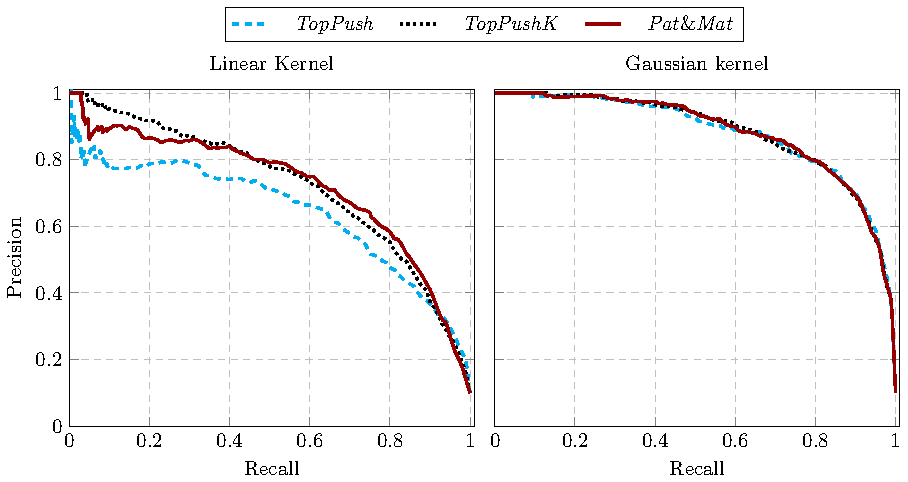
\includegraphics[width = \linewidth]{images/dual_results1.pdf}
  \caption{PR curves for all methods and  FashionMNIST dataset. The left column corresponds to the linear kernel~\eqref{eq:Linear kernel} and the right column corresponds to the Gaussian kernel~\eqref{eq:Gaussian kernel}.}
  \label{fig:PR comparison}
\end{figure}

For a better illustration of how the methods from Figure~\ref{fig:PR comparison} work, we present density estimates of scores $\bm s$ from \eqref{eq:defin_s}. High scores predict positive labels while low scores predict negative labels. The rows of Figure \ref{fig:Scores comparison} depict the linear \eqref{eq:Linear kernel} and the Gaussian kernels \eqref{eq:Gaussian kernel} with~$\sigma = 0.01$ while each column corresponds to one method. The black vertical lines depict the top 5\%-quantile of all scores (on the testing set). Since a smaller overlap of scores of samples with positive and negative labels implies a better separation, we deduce the benefit of the Gaussian over the linear kernel.

\begin{figure}[!ht]
  \centering
  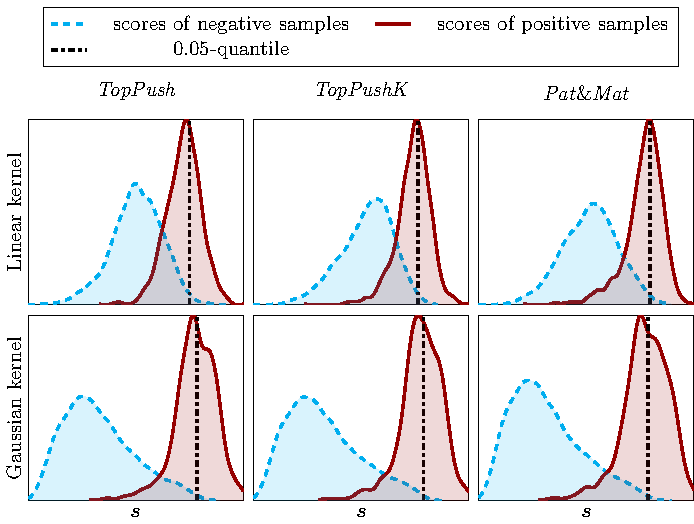
\includegraphics[width = \linewidth]{images/dual_results2.pdf}
  \caption{Density estimates for scores corresponding to samples with positive and negative labels for the FashionMNIST dataset.}
  \label{fig:Scores comparison}
\end{figure}

In Table~\ref{tab:Metrics comparison} we present the precision of all methods across all datasets from Table~\ref{tab:Datasets}. For each dataset, we trained each method and computed precision at certain levels of recall. The depicted values are averages over all datasets. For each kernel and each level of recall, the best precision is highlighted in light green. Moreover, the best overall precision for each level of recall is depicted in dark green. We can make several observations from Table~\ref{tab:Metrics comparison}:
\begin{itemize}
  \item All methods perform better with the Gaussian kernels than with the linear kernel. 
  \item \TopPush and \TopPushK perform better for sufficiently small recall. This happened because they consider the threshold to be the maximal $K$ negative scores and small recall corresponds to high threshold. However, for the same reason, \TopPush is not robust.
  \item \PatMat is the best for all kernels if the recall is sufficiently large. The reason is again the form of the decision threshold.
\end{itemize}

\begin{table}[ht]
  \caption{The precision of all methods averaged across all datasets from Table~\ref{tab:Datasets}. Each column represents precision at a certain level of recall. Light green depicts the best method for the given kernel and dark green depicts the best overall method.}
  \label{tab:Metrics comparison}
  \centering
  \begin{tabular}{@{}c|llllllll@{}}
    \toprule
    \multicolumn{3}{c}{} & \multicolumn{6}{c}{$\pratrec$}  \\
    \cmidrule(lr){4-9}
    \multicolumn{3}{c}{}
      & 0.05 & 0.1 & 0.2 & 0.4 & 0.6 & 0.8 \\
    \midrule
    \multirow{6}{*}{\rotatecell{Linear kernel}}
    & \TopPush
      & & \best 79.83 & 64.27 & \best 65.55 & 61.85 & 57.89 & 51.83 \\
    & \TopPushK & $K = 5$
      & 73.96 & \best 65.41 & 64.82 & 60.28 & 56.94 & 50.52 \\
    & & $K = 10$
      & 60.63 & 61.97 & 59.69 & 56.89 & 54.40 & 49.83 \\
    & \PatMat & $\tau = 0.01$
      & 63.67 & 60.30 & 58.74 & 57.75 & 53.32 & 48.42 \\
    & & $\tau = 0.05$
      & 54.05 & 60.91 & 63.32 & 55.24 & 52.55 & 48.30 \\
    & & $\tau = 0.1$
      & 57.02 & 61.24 & 62.49 & \best 63.11 & \best 59.91 & \best 52.14 \\
    \midrule
    \multirow{6}{*}{\rotatecell{Gaussian kernel}}
    & \TopPush
      & & \besttotal 97.50 & 86.06 & 81.28 & 76.15 & 71.13 & 60.17 \\
    & \TopPushK & $K = 5$
      & 92.50 & 87.56 & 85.31 & 78.47 & 70.77 & 57.10 \\
    & & $K = 10$
      & 89.50 & 87.56 & 83.15 & 79.09 & 71.88 & 59.27 \\
    & \PatMat & $\tau = 0.01$
      & 89.65 & \besttotal 89.11 & \besttotal 86.75 & 80.77 & 75.44 & 65.95 \\
    & & $\tau = 0.05$
      & 80.77 & 81.28 & 85.74 & 82.92 & 74.91 & 65.04 \\
    & & $\tau = 0.1$
      & 81.30 & 84.14 & 82.58 & \besttotal 83.12 & \besttotal 77.82 & \besttotal 66.50 \\
    \bottomrule
  \end{tabular}
\end{table}

In Figure~\ref{fig:Convergence comparison}, we investigate the convergence of methods. In each column, we show the convergence of primal and dual problems for one method. To solve the primal problem, we use the gradient method proposed in~\cite{adam2019patmat}. For the dual problem, we use our Algorithm~\ref{alg:Coordinate descent}. Since~\cite{adam2019patmat} considers only linear kernels, we present them. Moreover, since the computation of the objective is expensive, the results are presented for the sigillito1989classification dataset. We can see that \TopPush and \TopPushK converge to the same objective for primal and dual problems. This means that the problem was solved to optimality. However, there is a little gap between optimal solution of primal and dual problems for \PatMat.

\begin{figure}[!ht]
  \centering
  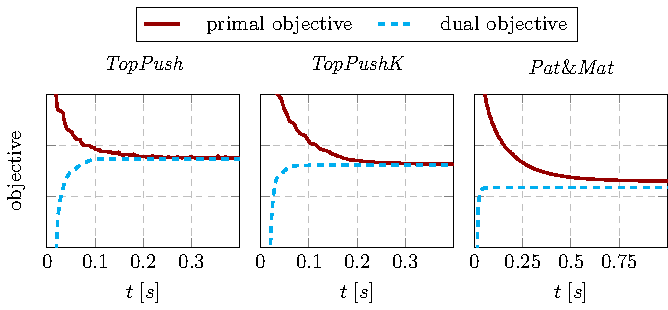
\includegraphics[width = \linewidth]{images/dual_results3.pdf}
  \caption{Convergence of the objectives for the primal (red line) and dual (blue line) problems for the sigillito1989classification dataset with linear kernel.}
  \label{fig:Convergence comparison}
\end{figure}

Finally, Table~\ref{tab:Time comparison} depicts the time comparison for all methods and all datasets. It shows the average time in milliseconds needed for one \repeatloop loop in Algorithm~\ref{alg:Coordinate descent}. The time is relatively stable and for most of the datasets it is below one millisecond. Since we run all experiments for 20000 \repeatloop loops, the evaluation of one method with one hyperparameter setting takes a few seconds for smaller datasets and approximately 7 minutes for FashionMNIST. The average time for one~$\Delta_l$ in step~\ref{alg: line 5} in Algorithm~\ref{alg:Coordinate descent} took between $1.7\cdot 10^{-7}$ and $3.1\cdot 10^{-7}$ seconds for each methods. It is almost the same for all datasets, which corresponds to the fact that the complexity of step~\ref{alg: line 5} is independent of the size of the dataset. Note that in all experiments we used precomputed kernel matrix~$\K$ saved on the hard drive and not in memory.

\begin{table}[ht]
    \caption{The average time with standard deviation (in milliseconds) for one \repeatloop loop in Algorithm~\ref{alg:Coordinate descent}. The average time for one~$\Delta_l$ in step~\ref{alg: line 5} in Algorithm~\ref{alg:Coordinate descent} took between $1.7\cdot 10^{-7}$ and $3.1\cdot 10^{-7}$ seconds for each methods.}
    \label{tab:Time comparison}
    \centering
    \begin{tabular}{@{}c|llll@{}}
        \toprule
        \multicolumn{2}{c}{}
          & \TopPush & \TopPushK & \PatMat \\
        \midrule
        \multirow{5}{*}{\rotatecell{One \repeatloop \\ loop [ms]}}
        & sigillito1989classification
          & $ 0.04 \pm 0.00 $ & $ 0.03 \pm 0.00 $ & $ 0.03 \pm 0.00 $ \\
        & Spambase
          & $ 0.56 \pm 0.02 $ & $ 0.49 \pm 0.01 $ & $ 0.50 \pm 0.01 $ \\
        & WhiteWineQuality
          & $ 0.62 \pm 0.03 $ & $ 0.53 \pm 0.01 $ & $ 0.54 \pm 0.01 $ \\
        & RedWineQuality
          & $ 0.17 \pm 0.01 $ & $ 0.14 \pm 0.01 $ & $ 0.15 \pm 0.01 $ \\
        & Fashion-MNIST
          & $ 17.16 \pm 0.74 $ & $ 15.95 \pm 0.14 $ & $ 15.54 \pm 0.80 $ \\
        \bottomrule
    \end{tabular}
\end{table}

\section{Conclusion}\label{sec:Conclusion}

In this paper, we analyzed and extended the general framework for binary classification on top samples from~\cite{adam2019patmat} to nonlinear problems. Achieved results can be summarized as follows:
\begin{itemize}
    \item We derived the dual formulations for \TopPush, \TopPushK and \PatMat.
    \item We proposed a new method for solving the dual problems. We performed its complexity analysis. For selected surrogate functions we also derived the exact formulas needed in the method.
    \item We performed a numerical analysis of the proposed method. We showed its good convergence as well as improved performance of nonlinear kernels over the linear one.
\end{itemize}
Based on the numerical analysis from Section~\ref{sec:Numerical experiments}, we recommend using \TopPush or \TopPushK for problems where the resulting recall should be small. Otherwise, we recommend using \PatMat with an appropriately selected~$\tau$ parameter.

\chapter{Deep}

Binary classifiers compute a score for each sample and compare it with a given threshold to predict whether the sample belongs to the positive or negative class. This score is often interpreted as the probability that the sample is of the positive class, and the threshold is usually $0.5$. Such a task attempts to classify all samples correctly.

On the other hand, many applications need to classify only a small fraction of samples correctly. In information retrieval systems, the user is interested only in the top few queries. Whenever samples undergo manual processing, humans can process only a small fraction of all samples. Cybersecurity defensive mechanisms must have extremely low false positive rates; otherwise, they are removed by the user. In all these applications, the score determines the sample relevance. After computing the scores of all samples, they are compared with a threshold. All samples below the threshold are irrelevant. The small fraction of samples above the threshold is deemed positive. These selected samples are then the search results, items for further analysis, or the detected malware.

Since this task considers only scores above the threshold, \cite{boyd2012accuracy} named it \AccatTop. The important distinction from standard classifiers is that this threshold is no longer fixed, as in the case of $0.5$, but depends on all samples. Therefore, the objective is non-additive and non-decomposable. This brings both theoretical and numerical issues. Standard machine learning algorithms use minibatch sampling. However, when the threshold is computed on a minibatch, it provides a lower estimate of the true threshold. Therefore, the sampled threshold is a biased estimate of the true threshold. Figure~\ref{fig:thresholds1} illustrates this phenomenon. The bias between the true and sampled thresholds is large even for medium-sized minibatches. Backpropagation then propagates this sampling error through the whole gradient, and consequently, the minibatch gradient is a biased estimate of the true gradient. This brings numerical issues \cite{bottou2018optimization}.

\begin{figure}[!ht]
  \centering
  \begin{tikzpicture}
    \begin{axis}[
      height=130,
      width=0.9\linewidth,
      title = {},
      xlabel = {Minibatch size},
      ylabel = {},
      ymin = 1.5,
      ymax = 2.5,
      tick pos = left,
      grid = major,
      grid style = {dashed, draw = gray!50, very thin},
      enlargelimits = false,
      legend pos=south east,
      legend cell align={left},
    ]
      \addplot [lineD]  table[x index=0, y index=1] {\Quantiles};
      \addlegendentry{True threshold}
      \addplot [lineA] table[x index=0, y index=2] {\Quantiles};
      \addlegendentry{Sampled threshold}
      \addplot [myblue!50,name path=path1] table[x index=0, y index=3] {\Quantiles};
      \addplot [myblue!50,name path=path2] table[x index=0, y index=4] {\Quantiles};
      \addplot[myblue!50,fill opacity=0.5] fill between[of=path1 and path2]; \addlegendentry{Standard deviation}
    \end{axis}
  \end{tikzpicture}
  \caption{The bias between the sampled and true thresholds computed from scores following the standard normal distribution. The threshold separates the top $1\%$ of samples with the highest scores.}
  \label{fig:thresholds1}
\end{figure}

\begin{figure*}[!ht]
  \centering
  \begin{tikzpicture}
    \begin{axis}[
      width = \textwidth,
      height = 5cm, 
      xmin = -0.525,
      xmax = 2.05,
      ymin = -0.25,
      ymax = 3.25,
      hide axis,
      legend style = {
        column sep = 10pt,
        legend columns = 4,
        legend cell align = {left},
        anchor = south,
        at = {(0.5, 1.05)},
      },
      enlargelimits = false,
    ]
      \addplot [scatterneg] table[x index=1, y index=0] {\ExampleTop};
      \addlegendentry{Negative scores}
      \addplot [scatterpos] table[x index=3, y index=2] {\ExampleTop};
      \addlegendentry{Positive scores}
      \addlegendimage{black, very thick, dashed}
      \addlegendentry{Threshold accuracy}    
      \addlegendimage{myorange, very thick, dashed}
      \addlegendentry{Threshold top}    
      \addplot [scatterneg] table[x index=5, y index=4] {\ExampleTop};
      \addplot [scatterpos] table[x index=7, y index=6] {\ExampleTop};
      \node [draw, left] at (axis cs:-0.05,2.5) {\parbox{2cm}{\textbf{Classifier 1} \\ Accuracy 95\% \\ Top 19\%}};
      \node [draw, left] at (axis cs:-0.05,0.5) {\parbox{2cm}{\textbf{Classifier 2} \\ Accuracy 76\% \\ Top 53\%}};
      \draw [black, very thick, dashed] (axis cs:1, 1.75) -- (axis cs:1,3.25);
      \draw [myorange, very thick, dashed] (axis cs:1.764, 1.75) -- (axis cs:1.764,3.25);
      \draw [black, very thick, dashed] (axis cs:0.995,-0.25) -- (axis cs:0.995,1.25);
      \draw [myorange, very thick, dashed] (axis cs:1,-0.25) -- (axis cs:1,1.25);
      \draw [black, very thick] (axis cs:-0.525,1.5) -- (axis cs:2.05,1.5);
      \end{axis}
  \end{tikzpicture}
  \caption{Difference between standard classifiers (top row) and classifiers maximizing accuracy at the top (bottom row). While the former has a good total accuracy, the latter has a good top acccuracy.}
  \label{fig:difference}
\end{figure*}

Our method mitigates this bias. It is based on several results. \cite{li2014top} proposed the TopPush formulation of the accuracy at the top and solved it in its dual formulation. \cite{adam2019patmat} solved the TopPush formulation directly in its primal form for linear classifiers. Since we generalize the linear TopPush into non-linear classifiers, we name our method \DeepTopPush. We stay in the primal form to be able to employ stochastic gradient descent. Due to non-decomposability, we need to propose a way of computing the gradient and reduce the bias mentioned above. Since the threshold always equals to one of the scores \cite{boyd2012accuracy}, its computation has a simple local formula. We implicitly remove some variables and apply the chain rule (backpropagation) to compute the gradient in an end-to-end manner. To reduce the bias, we need to improve the approximation quality of the sampled threshold. We employ again the fact that the true threshold corresponds to one sample. Since this sample changes slowly during optimization, we modify the idea of \cite{adam2019machine} and enhance the current minibatch by the sample, which equalled the sampled threshold on the previous minibatch. As this added sample usually propagates across multiple minibatches, it tracks the threshold, and this trick mitigates the sampled threshold bias. The main contributions of the paper are as follows:
\begin{itemize}
  \item We propose \DeepTopPush, which is a simple and scalable method for accuracy at the top.
  \item We show that \DeepTopPush increases the computational time only slightly, yet it achieves better performance than prior art methods.
  \item We show both theoretically and numerically that enhancing the minibatch by one sample reduces the bias of the sampled gradient.
\end{itemize}
The paper is organized as follows: Section \ref{sec:deeptheory} introduces a general formulation of accuracy at the top. Section \ref{sec:solving} derives formulas for the bias of the sampled threshold and proposes \DeepTopPush to minimize it. Section \ref{sec:numerics} shows the good performance of \DeepTopPush on multiple images recognition datasets, a real-world medical application, and a malware detection dataset, where we detected 46\% malware at an extremely low false alarm rate of $10^{-5}$. To promote reproducibility, our codes are available online.

\section{Accuracy at the top}\label{sec:deeptheory}

This section introduces the accuracy at the top. A standard deep network $f$ with weights $\bm{w}$ takes inputs $\bm{x}_i$, transforms them into scores $z_i$, and computes the total loss based on these scores and labels $y_i$. On the other hand, accuracy at the top solves
\begin{equation}\label{eq:problem}
  \begin{aligned}
    \minimize{w,z,t}
    & \lambda_1 \sum_{i\in I^-}\II_{z_i \ge t} + \lambda_2\sum_{i\in I^+}\II_{z_i < t} \\
    \st
    & z_i = f(\bm{w};\bm{x}_i), \\
    & t = G(\{(z_i, y_i)\}_{i\in I}).
  \end{aligned}
\end{equation}
Similarly to the standard network, the classifier $f$ computes the score $z_i$ for each sample $\bm{x}_i$. Then a general function $G$ takes the scores and labels of \textbf{all} samples and computes the threshold $t$. This makes the problem non-decomposable. The objective function equals the weighted sum of false-positives (negative samples above the threshold) and false-negatives (positive samples below the threshold). Here, $I$, $I^+$ and $I^-$ are the sets of all, positive and negative labels, respectively, and $\II$ is the characteristic ($0/1$) function counting how many times the argument is satisfied. Setting \eqref{eq:problem} includes TopPush \cite{li2014top} which minimizes the number of positive samples below the highest-ranked negative sample. This fits into \eqref{eq:problem} with $\lambda_1=0$, $\lambda_2=1$ and $t=\max_{i\in I^-} z_i$.

Figure \ref{fig:difference} shows the difference between the standard approach with cross-entropy and accuracy at the top. While classifier 1 has good total accuracy, its top accuracy is subpar because of the few negative outliers. On the other hand, classifier 2 has worse total accuracy, but its top accuracy is extremely good because more than half of the positive samples are on the top. While classifier 1 selected different thresholds for the accuracy and top metrics, these thresholds coincide for classifier 2.

Table \ref{table:summary} shows other special cases of \eqref{eq:problem} including maximizing precision at a given level of recall \cite{mackey2018constrained} or recall at $K$. The threshold $t$ always equals to the sample with the $j^*$-th highest score on all, positive, or negative samples. The problems differ only in $j^*$ and from which samples the threshold is computed. For example, Pat\&Mat-NP \cite{adam2019patmat} minimizes the false negative rate (equivalently maximizes the true positive rate) under the constraint that the false positive rate is at most $\tau$.

\begin{table}[!ht]
  \centering
  \begin{tabular}{@{}llllll@{}}
    \toprule
    Name & $\lambda_1$ & $\lambda_2$ & $t$ computed from & $j^*$ \\
    \midrule
    Prec@Rec    & $1$ & $0$ & positive samples & $n^+\tau$ \\
    Rec@K       & $0$ & $1$ & all samples      & $K$ \\
    TopPush     & $0$ & $1$ & negative samples & $1$ \\
    Pat\&Mat-NP & $0$ & $1$ & negative samples & $n^-\tau$ \\
    \bottomrule
  \end{tabular}
  \caption{Selected problems of setting \eqref{eq:problem}. False-positives and false-negatives have weights $\lambda_1$ and $\lambda_2$, the threshold $t$ equals to the sample with the $j^*$-th highest score on all, positive, or negative samples.}
  \label{table:summary}
\end{table}

\subsection{Related works}

There is a close connection between accuracy at the top and ranking problems \cite{batmaz2019review,werner2019review}. This was, together with similarities to the Neyman-Pearson problem, showed in \cite{adam2019patmat}. A special case of the ranking problems attempts to rank positive samples above negative samples. Several approaches, such as RankBoost~\cite{freund2003efficient}, Infinite Push~\cite{agarwal2011infinite} or $p$-norm push~\cite{rudin2009pnorm} employ a positive-negative pairwise comparison of scores, which can handle only small datasets. TopPush~\cite{li2014top} converts the pairwise sum into a single sum and minimizes the false-negatives below a threshold given by the maximum score corresponding to negative samples. Thus, it converts ranking into accuracy at the top problems.

Two approaches for solving \eqref{eq:problem} exist. The first approach considers the threshold constraint as it is, while the second approach uses heuristics to approximate it. In the first approach, Acc@Top~\cite{boyd2012accuracy} argues that the threshold equals one of the scores. They fix the index of a sample and solve as many optimization problems as there are samples. \cite{eban2017scalable,adam2019patmat,kumar2021implicit} write the threshold as a constraint and replace both the objective and the constraint via surrogates. \cite{eban2017scalable} uses Lagrange multipliers to obtain a minimax problem, \cite{mackey2018constrained} implicitly removes the threshold as an optimization variable and uses the chain rule to compute the gradient while \cite{macha2020nonlinear} solves an SVM-like dual formulation with kernels. \cite{grill2016learning} uses the same formulation but applies surrogates only to the objective and recomputes the threshold after each gradient step. TFCO \cite{cotter2019optimization} solves a general class of constrained problems via a minimax reformulation. In the second approach, SoDeep \cite{engilberge2019sodeep} or SmoothI \cite{thonet2021smoothi} use the fact that the threshold may be easily computed from sorted scores. They approximate the sorting operator by a network trained on artificial data. AP-Perf \cite{fathony2019ap} considers a general metric and hedges against the worst-case perturbation of scores. The authors argue that the problem is bilinear in scores and use duality arguments. However, the bilinearity is lost when optimizing with respect to the weights of the original network. 

\section{DeepTopPush as a method for maximizing accuracy at the top}\label{sec:solving}

This section first shows a basic algorithm to solve \eqref{eq:problem}. We then argue that the stochastic gradient descent produces a biased estimate of the true gradient, and we mention two strategies for mitigating this bias. Based on one strategy, we propose the \DeepTopPush algorithm. The whole section assumes that the classifier $f$ is differentiable.

\subsection{Basic algorithm for solving accuracy at the top}

Even though the presented technique can be applied to any formulation from Table \ref{table:summary}, for simplicity, we derive it only for the TopPush formulation, where $\lambda_1=0$ and $\lambda_2=1$. This amounts to minimizing the false-negatives in \eqref{eq:problem}. Since the function $\II$ in the formulation \eqref{eq:problem} is discontinuous, it is usually replaced by a general surrogate function $l$ which is continuous and non-decreasing. This leads to
\begin{equation}\label{eq:problem_surr1}
  \begin{aligned}
    \minimize{w,z,t}
    & \frac{1}{n^+}\sum_{i\in I^+}l(t-z_i) \\
    \st
    & z_i = f(\bm{w};\bm{x}_i), \\
    & t   = G(\{(z_i, y_i)\}_{i\in I}).
\end{aligned}
\end{equation}
To apply the stochastic gradient descent, we need to compute the gradient. The core idea follows \cite{mackey2018constrained} which was proposed in a more general context in \cite{adam2019machine}. It rewrites problem \eqref{eq:problem_surr1} into its equivalent form
\begin{equation}\label{eq:problem_surr2}
  \minimize{w}
  \frac{1}{n^+}\sum_{i\in I^+}l\Brac{G\Brac{\{(f(\bm{w};\bm{x}_j), y_j)\}_{j\in I}} - f(\bm{w};\bm{x}_i)}.
\end{equation}
This form removed the constraints and it has the advantage that the only optimization variable is $\bm{w}$ instead of $(\bm{w}, \bm{z}, t)$ in \eqref{eq:problem_surr1}. In all cases from Table \ref{table:summary}, the threshold $t$ always equals to one of the scores, let it have index $j^*$ and then $t=z_{j^*}$. Denoting the objective of \eqref{eq:problem_surr2} by $L(\bm{w})$, the chain rule implies that the gradient of the objective from \eqref{eq:problem_surr2} equals to
\begin{equation}\label{eq:grad1}
  \nabla L(\bm{w}) = \frac{1}{n^+} \sum_{i\in I^+}l'(t-z_i)\big(\nabla_w f(\bm{w};\bm{x}_{j^*}) - \nabla_w f(\bm{w};\bm{x}_i)\big).
\end{equation}
The stochastic gradient descent replaces the sum over all positive samples $I^+$ with a sum over all positive samples in a minibatch $\Imin^+$. However, as both the threshold $t$ and the index $j^*$ depend on all scores $z_i$, they need to be approximated on the minibatch as well. We denote these approximations by $\hat t$ and $\hat j$, respectively. Denoting the number of positive samples in the minibatch by $\nmin^+$, we replace the true gradient \eqref{eq:grad1} by the \textit{sampled gradient}
\begin{equation}\label{eq:grad2}
  \nabla \hat L = \frac{1}{\nmin^+}\sum_{i\in \Imin^+}l'(\hat t-z_i)\big(\nabla_w f(\bm{w};\bm{x}_{\hat j}) - \nabla_w f(\bm{w};\bm{x}_i) \big),
\end{equation}
The most straightforward way is to choose the sampled threshold $\hat t$ by the same rule as the true threshold $t$. As an example, if $t$ is the $100^{\rm th}$ largest score on the whole dataset and $\frac{n}{\nmin}=20$ is the ratio of sizes of the whole dataset and of the minibatch, we select the sampled threshold $\hat t$ as the $5^{\rm th}$ largest score on the minibatch. We summarize this procedure in Algorithm \ref{alg1}.

\begin{figure*}
  \begin{minipage}{0.48\textwidth}
    \begin{algorithm}[H]
      \centering
      \begin{algorithmic}[1]
        \State Initialize weights $\bm{w}$
        \Repeat
        \State Select minibatch $\Imin$
        \State \phantom{$\Iminh$}
        \State Compute $z_i\gets f(\bm{w};\bm{x}_i)$ for $i\in\Imin$
        \State Set $\hat t \gets G(\{(z_i,y_i)\}_{i\in\Imin})$
        \State 
        \State Compute $\nabla \hat L$ based on $\Imin$\phantom{$\Iminh$}
        \State Make a gradient step
        \Until{stopping criterion is satisfied}
      \end{algorithmic}
      \caption{Basic algorithm for solving \eqref{eq:problem} \\}
      \label{alg1}
    \end{algorithm}
  \end{minipage}
  \hfill
  \begin{minipage}{0.48\textwidth}
    \begin{algorithm}[H]
      \centering
      \begin{algorithmic}[1]
        \State Initialize weights $\bm{w}$, random index $j^*$
        \Repeat
        \State Select minibatch $\Imin$
        \State Enhance minibatch $\Iminh = \Imin \cup \{j^*\}$
        \State Compute $z_i\gets f(\bm{w};\bm{x}_i)$ for $i\in\Iminh$
        \State Set $\hat t \gets \{\max z_i \mid i\in \Iminh \cap I^-\}$
        \State Find index $j^*$ such that $t = z_{j^*}$
        \State Compute $\nabla \hat L$ based on $\Iminh\cap I^+$
        \State Make a gradient step
        \Until{stopping criterion is satisfied}
      \end{algorithmic}
      \caption{DeepTopPush as an efficient method for maximizing accuracy at the top.}
      \label{alg2}
    \end{algorithm}
  \end{minipage}
\end{figure*}

\subsection{Bias of the sampled gradient}

Convergence proofs of the stochastic gradient descent require that the sampled gradient is an unbiased estimate of the true gradient \cite{bottou2018optimization}. This means that
\begin{equation}\label{eq:defin_bias}
  \bias(\bm{w}) := \nabla L(\bm{w}) - \EE \nabla \hat L(\bm{w})
\end{equation}
equals to $0$ for all $\bm{w}$. A comparison of \eqref{eq:grad1} and \eqref{eq:grad2} shows that a necessary condition is that the sampled threshold $\hat t$ is an unbiased estimate of the true threshold $t$. However, the sampled version underestimates the true value, which is evident for the maximum where the sampled maximum is always smaller or equal to the true maximum. The next result quantifies the difference between the sampled and true thresholds.

\begin{proposition}[\cite{glynn1996importance}]\label{proposition:bound}
  Let $X$ be an absolutely continuous random variable with distribution function $F$, let $X_1,\dots,X_n$ be iid samples from $X$ and let $\tau\in(0,1)$. Denote the true threshold $t=F^{-1}(1-\tau)$ and the sampled threshold $\hat t=X_{[\lceil n\tau\rceil]}$. If $F$ is differentiable with a positive gradient at $t$, then
  \begin{equation*}
    \sqrt{n}(t - \hat t) \rightarrow N\left(0, \frac{\tau(1-\tau)}{F'(t)^2}\right),
  \end{equation*}
  where the convergence is in distribution and $N$ denotes the normal distribution.
\end{proposition}

This proposition states that when the minibatch size increases to infinity, the variance of the sampled threshold is approximately $\frac{\tau(1-\tau)}{nF'(t)^2}$. Figure \ref{fig:thresholds1} in the introduction shows this empirically for the case where the scores follow the standard normal distribution and $\tau=0.01$ is the desired top fraction. The approximation is poor with both large bias and standard deviation. Even though this result gives us insight into the bias of the sampled threshold, we are ultimately interested in the bias of the sampled gradient $\nabla \hat L(\bm{w})$. To do so, recall that $j^*$ is the threshold index on the whole dataset ($t=z_{j^*}$) while $\hat j$ is the threshold index on the minibatch ($\hat t=z_{\hat j}$). We split the computation based on whether these two indices are identical.

\begin{lemma}\label{lemma:convergence}
  Let $j^*$ be unique. Assume that the selection of positive and negative samples into the minibatch is independent and that the threshold is computed from negative samples while the objective is computed from positive samples. Then the conditional expectation of the sampled gradient satisfies
  \begin{equation*}
    \EE\Brac{\nabla \hat L(\bm{w}) \mid \hat j=j^*} =  \nabla L(\bm{w}).
  \end{equation*}
\end{lemma}
\begin{proof}
  If $j^*$ is unique, then the true threshold $t$ is a differentiable function. The differentiability of $L$ and $\hat L$ follows from the chain rule. If $\hat j=j^*$ holds, then the sampled gradient equals to
  \begin{equation}\label{eq:grad_min_aux}
    \nabla \hat L(\bm{w})= \frac{1}{\nmin^+}\sum_{i\in \Imin^+}l'(t-z_i)\big(\nabla_w f(\bm{w};\bm{x}_{j^*}) - \nabla_w f(\bm{w};\bm{x}_i) \big).
  \end{equation}
  The summands are identical to the ones in \eqref{eq:grad1}. Since the sum is performed with respect to positive samples, the threshold is computed from negative samples, the lemma statement follows.
\end{proof}

Now we present the main result about the bias.

\begin{theorem}\label{theorem:convergence}
  Under the assumptions of Lemma \ref{lemma:convergence}, the bias of the sampled gradient from \eqref{eq:defin_bias} satisfies
  \begin{equation}\label{eq:comp_bias}
    \bias(\bm{w}) = \PP(\hat j\neq j^*) \Brac{\nabla L(\bm{w}) - \EE\Brac{\nabla \hat L(\bm{w}) \mid \hat j\neq j^*}}.
  \end{equation}
\end{theorem}
\begin{proof}
  The law of total expectation implies
  \begin{equation*}
    \begin{aligned}
      \EE \nabla \hat L(\bm{w})
      & = \PP(\hat j=j^*)\EE(\nabla \hat L(\bm{w}) \mid \hat j=j^*) \\
      & \qquad + \PP(\hat j\neq j^*)\EE(\nabla \hat L(\bm{w}) \mid \hat j\neq j^*),
    \end{aligned}
  \end{equation*}
  from where the statement follows due to definiton \eqref{eq:defin_bias} and Lemma \ref{lemma:convergence}.
\end{proof}

The assumptions of Theorem \ref{theorem:convergence} holds for all methods from Table \ref{table:summary} with the exception of Rec@K. For this method, the bias contains an additional term, as we show in the appendix.

The bias \eqref{eq:comp_bias} consists of a multiplication of two terms. We propose two strategies for reducing the bias. The first strategy reduces both terms, while the second strategy reduces only the first term.

\subsection{Bias reduction: Increasing minibatches size}\label{sec:bias1}

The natural choice to mitigate the bias is to work with large minibatches. Even though this is not a standard way, some works suggest this route \cite{you2019large}. When the minibatch is large, it contains more samples and the chance that $\hat j$ differs from $j^*$ decreases. This reduces the first term in~\eqref{eq:comp_bias}. Moreover, Proposition \ref{proposition:bound} ensures that the difference between the sampled threshold $\hat t$ and the true threshold $t$ is small. Then the difference between the true gradient \eqref{eq:grad1} and the sampled gradient \eqref{eq:grad2} decreases as well. This reduces the second term in \eqref{eq:comp_bias}. This approach is applicable to any method from Table~\ref{table:summary}.

\subsection{Bias reduction: Incorporating delayed values}\label{sec:bias2}

Various reasons may enforce the use of small minibatches. Then Algorithm \ref{alg1} is not suitable for a small fraction of top samples. For example, a minibatch of size $32$ with $16$ negative samples must have thresholds $\tau\ge \frac{100}{16}=6.25\%$. However, we need to aim for much smaller thresholds.

We propose a simple fix based on the reasoning that when the weights $\bm{w}$ of a neural network are updated, the scores $\bm{z}$ usually do not change much, especially for a small learning rate. This means that if a sample has the largest score, it will likely have the largest score even after the gradient step. Since the threshold $t$ for TopPush equals the largest score corresponding to negative samples, we can easily track it. We enhance the current minibatch by the negative sample from the previous minibatch with the highest score. This significantly increases the chance that the sampled threshold is the true threshold and, due to the first term in \eqref{eq:comp_bias}, reduces the bias of the sampled gradient.

We summarize the procedure in Algorithm \ref{alg2} and show it next to Algorithm \ref{alg1} to highlight the differences. In every iteration, it stores the index $j^*$ of the sample, which equals the threshold (step~7). We add it to the enhanced minibatch (step 4). Since we can track only the maximum, we set the threshold as the maximum of scores from negative samples (step~6) and minimize false-positives. Since Algorithm \ref{alg2} uses the same formulation as \textit{TopPush} \cite{li2014top} but can handle an arbitrary classifier, we name it \DeepTopPush. We provide empirical evidence of why our technique works later in Section \ref{sec:delay}.

\section{Numerical experiments}\label{sec:numerics}

This section presents numerical results for \DeepTopPush. Table \ref{table:summary} shows that it is similar to \PatMatNP. While the former maximizes the number of positives above the largest negative, while the latter maximizes the number of positives above the $n^-\tau$-largest negative. The former may be understood as requiring no false-positives, while the latter allows for false positive rate $\tau$.

Section \ref{sec:bias1} showed that we can use large minibatches to obtain good results for \PatMatNP for small fractions of top samples $\tau$. Section~\ref{sec:bias2} showed that \DeepTopPush works well even with small minibatches if we track the threshold by enhancing the minibatch by one sample. We present numerical comparisons in several sections, each with a different purpose. Comparison with the prior art \TFCO and \APPerf is performed on several visual recognition datasets and shows that \DeepTopPush outperforms other methods. Then we present two real-world applications. The first one shows that \DeepTopPush can handle ranking problems. The second one presents results on a complex malware detection problem. Finally, we show similarities between \DeepTopPush and \PatMatNP and explain why enhancing the minibatch in Algorithm \ref{alg2} works.

\subsection{Dataset description and Computational setting}\label{sec:set}

We consider the following image recognition datasets: FashionMNIST~\cite{xiao2017fashionmnist}, CIFAR100~\cite{krizhevsky2009learning}, SVHN2~\cite{netzer2011reading} and ImageNet~\cite{russakovsky2015imagenet}. These datasets were converted to binary classification tasks by selecting one class as the positive class and the rest as the negative class. ImageNet merged turtles and non-turtles. We also consider the 3A4 dataset~\cite{ma2015deep} with molecules and their activity levels. Finally, malware analysis reports of executable files were provided by a cybersecurity company. This is an extremely tough dataset as individual samples are JSON files whose size ranges from 1kB to 2.5MB. Moreover, they contain different features, and their features may have variable lengths. All datasets are summarized in the appendix.

We use truncated quadratic loss~$l(z) = (\max\{0, 1 + z\})^2$ as the surrogate function and $\tau=\frac{1}{n^-}$ and $\tau=0.01$. This first one computes the true positive rate above the second highest-ranked negative, while the latter allows for the false positive rate of $1\%$. All algorithms were run for $200$ epochs on an NVIDIA P100 GPU card with balanced minibatches of 32 samples. The only exception was Malware Detection, which was run on a cluster in a distributed manner, and where the minibatch size was $20000$. For the evaluation of numerical experiments, we use the standard receiver operating characteristic (ROC) curve. All results are computed from the test set. All codes were implemented in the Julia language~\cite{bezanson2017julia}. The network structure was the same for all methods; we describe them in the online appendix.

\subsection{Comparison with prior art}\label{sec:comparison}

We compare our methods with \BaseLine, which uses the weighted cross-entropy. Moreover, we use two prior art methods which have codes available online, namely \TFCO \cite{cotter2019optimization,narasimhan2019optimizing} and \APPerf \cite{fathony2019ap}. We did not implement the original TopPush because its duality arguments restrict the classifiers to only linear ones. Table \ref{table:time} shows the time requirement per epoch. All methods besides \APPerf have similar time requirements, while \APPerf is much slower. This difference increases drastically when the minibatch size increases, as noted in \cite{fathony2019ap}. We do not present the results for SVHN for \APPerf because it was too slow and for \TFCO because we encountered a TensorFlow memory error. All these methods are designed to maximize true-positives when the false positive rate is at most $\tau$. This is the same as for \PatMatNP.

\begin{table}[!ht]
  \centering
  \begin{tabular}{@{}llll@{}}
      \toprule      
       & FashionMNIST & CIFAR100 & SVHN \\
      \midrule
      BaseLine
        & 4.4s & 5.1s & 62.8s \\
      DeepTopPush
        & 4.8s & 5.6s & 66.6s \\
      Pat\&Mat-NP
        & 4.8s & 5.6s & 66.6s \\
      TFCO
        & 7.2s & 6.5s & - \\
      AP-Perf
        & 95.3s & 81.2s & - \\
      \bottomrule
  \end{tabular}
  \caption{Time requirements per epoch for investigated methods for minibatches of size $\nmin=32$.}
  \label{table:time}
\end{table}

\begin{table*}[ht]
  \centering
  \footnotesize
  \begin{tabular}{@{}c|llllll@{}}
    \toprule
    & \thead{Dataset}
    & \thead{BaseLine}
    & \thead{DeepTopPush}
    & \thead{Pat\&Mat-NP}
    & \thead{TFCO}
    & \thead{AP-Perf} \\
    \midrule
    \multirow{4}{*}{\rotatebox[origin=c]{90}{\parbox[c]{1.5cm}{\centering tpr@fpr $\tau=\nicefrac{1}{n^-}$}}}
    & FashionMNIST
      & $5.06 \pm 1.41$
      & \best $27.30 \pm 5.91$
      & $22.21 \pm 5.62$
      & $11.30 \pm 3.44$
      & $9.90$ \\
    & CIFAR100
      & $1.70 \pm 0.46$
      & \best $14.40 \pm 5.44$
      & $8.10 \pm 3.45$
      & $7.70 \pm 2.28$
      & $5.00$ \\
    & 3A4
      & $2.58 \pm 0.61$ 
      & \best $5.61 \pm 1.70$
      & $3.79 \pm 0.90$
      & $3.03 \pm 1.52$
      & $3.03$ \\
    & SVHN
      & $6.51 \pm 1.37$
      & \best $12.21 \pm 5.39$
      & $12.07 \pm 4.41$ 
      & - & -\\
    \midrule
    \multirow{4}{*}{\rotatebox[origin=c]{90}{\parbox[c]{1.5cm}{\centering tpr@fpr $\tau=0.01$}}}
    & FashionMNIST
      & $63.14 \pm 1.39$
      & \best $75.37 \pm 1.18$
      & $74.11 \pm 1.00$
      & $73.27 \pm 2.92$
      & $64.60$ \\
    & CIFAR100
      & $49.40 \pm 4.90$
      & \best $70.20 \pm 2.14$
      & $66.30 \pm 2.33$
      & $67.30 \pm 1.79$
      & $65.00$ \\
    & 3A4
      & $57.80 \pm 0.35$ 
      & $60.08 \pm 3.35$
      & \best $65.91 \pm 0.59$
      & $54.55 \pm 10.22$
      & $63.64$ \\
    & SVHN
      & $84.72 \pm 0.84$
      & $91.05 \pm 1.45$
      & \best $91.07 \pm 0.30$
      & - & - \\
    \bottomrule
  \end{tabular}
  \caption{The true positive rates (in \%) at two levels of false positive rates averaged across ten indepenedent runs with standard deviation. The best methods are highlighted.}
  \label{tab:Overall comparison}
\end{table*}

Table \ref{tab:Overall comparison} shows the true positive rate (tpr) above the second-largest negative and at the prescribed false positive rate (fpr) $\tau=0.01$. Using the second-largest negative, which corresponds to $\tau=\frac{1}{n^-}$, allows for one outlier. The results are averaged over ten independent runs except for AP-Perf, which is too slow. The best result for each metric (in columns) is highlighted. All methods are better than \BaseLine. This is not surprising as all these methods are designed to work well for low false positive rates. \DeepTopPush outperforms all other methods at the top, while it performs well at the low fpr of $\tau=0.01$. There \PatMatNP, which also falls into our framework, performs well. Both these methods outperform the state of the art methods. 

Figure \ref{fig: roc curves} \textbf{A)} shows the ROC curves on CIFAR100 averaged over ten independent runs. We use the logarithmic $x$ axis to highlight low fpr modes. \DeepTopPush performs significantly the best again whenever the false positive rate is smaller than $0.01$.

As a further test, we performed a simple experiment on ImageNet. We modified the pre-trained EfficientNet B0 \cite{tan2019efficientnet} by removing the last dense layer and adding another dense layer with one output. Then we retrained the newly added layer to perform well at the top. The original EfficientNet achieved $68.0\%$ at the top, while \DeepTopPush achieved $70.0\%$ for the same metric. This shows that \DeepTopPush can provide better accuracy at the top than pre-trained networks.

\subsection{Application to ranking}

The 3A4 dataset contains information about activity levels of approximately $50000$ molecules, each with about $10000$ descriptors. The activity level corresponds to the usefulness of the molecule for creating new drugs. Since medical scientists can focus on properly investigating only a small number of molecules, it is important to select a small number of molecules with high activity.

We converted the continuous activity level into binary by considering a threshold on the activity. Since the input is large-dimensional, and there is no spatial structure to use convolutional neural networks, we used PCA to reduce the dimension to $100$. Then we created a network with two hidden layers and applied \DeepTopPush to it. The test activity was evaluated at the continuous (and not binary level). Table \ref{tab:Overall comparison} shows again the results at the top. \DeepTopPush outperforms other methods. Figure \ref{fig:molecules} shows that high scores (output of the network) indeed correspond to high activity. Thus, even though the problem was ``binarized'' and its dimension reduced, our algorithm was able to select a small number of molecules with high activity levels. These molecules can be used for further manual (expensive) investigation.

\begin{figure}[!ht]
  \centering
  \begin{tikzpicture}
    \begin{axis}[
      width=0.8\linewidth,
      title = {},
      xlabel = {Scores},
      ylabel = {Activity},
      xmax = 8,
      ymax = 8.5,
      tick pos = left,
      grid = major,
      grid style = {dashed, draw = gray!50, very thin},
      enlargelimits = false,
    ]
      \addplot [scatterneg] table[x index=0, y index=1] {\Molecules};
      \addplot [scatterpos] table[x index=2, y index=3] {\Molecules};
      \node[circle, black, draw, very thick, minimum size = 30pt, label = above left:Target] at (axis cs:5.2,7.55) {};
      \end{axis}
  \end{tikzpicture}
  \caption{Results for the 3A4 dataset. The goal was to assign large scores to a few molecules with high activity (scores on top-right are preferred).}
  \label{fig:molecules}
\end{figure}

\begin{figure*}[!ht]
  \centering
  \begin{tikzpicture}
    \begin{groupplot}[
      group style = {
          group size = 2 by 1,
          horizontal sep = 20pt,
          x descriptions at = edge bottom,
          y descriptions at = edge left,
      },
      footnotesize,
      width= 0.4\linewidth,
      xlabel = {False positive rate},
      ylabel = {True positive rate},
      ytick = {0, 0.2, 0.4, 0.6, 0.8, 1},
      ymin = -0.05,
      xmode = log,
      tick pos = left,
      grid = major,
      grid style = {dashed, draw = gray!50, very thin},
      enlargelimits = false,
      height = 150,
    ]
    \nextgroupplot[
      title = {\textbf{A)} CIFAR100},
      xmin = 0.001,
      legend to name={CommonLegend},
      legend style = {
          column sep = 10pt,
          legend columns = 3,
          legend cell align = {left},
      }
    ]
      % legend
      \addlegendimage{lineDeepTP}
      \addlegendentry{DeepTopPush}
      \addlegendimage{lineBaseLine}
      \addlegendentry{BaseLine}
      \addlegendimage{lineTFCO}
      \addlegendentry{TFCO($\tau = 10^{-2}$)}
      \addlegendimage{lineAPPerf}
      \addlegendentry{AP-Perf($\tau = 10^{-2}$)}
      \addlegendimage{linePatMat3}
      \addlegendentry{Pat\&Mat-NP($\tau = 10^{-3}$)}
      \addlegendimage{linePatMat2}
      \addlegendentry{Pat\&Mat-NP($\tau = 10^{-2}$)}

      \addplot [lineDeepTP] table[x index=2, y index=3] {\DeepCIFAR};
      \addplot [lineTFCO] table[x index=12, y index=13] {\DeepCIFAR};
      \addplot [lineBaseLine] table[x index=0, y index=1] {\DeepCIFAR};
      \addplot [lineAPPerf] table[x index=8, y index=9] {\DeepCIFAR};
      \draw (axis cs:0.01,-0.05) -- (axis cs:0.01,1) node [right] at (axis cs:0.01,0.3) {Optimized threshold};

    \nextgroupplot[
      title = {\textbf{B)} Malware detection},
      xmin = 0.00001,
    ]
      \addplot [lineDeepTP]  table[x index=4, y index=5] {\DeepLarge};
      \addplot [linePatMat3]  table[x index=6, y index=7] {\DeepLarge};
      \addplot [linePatMat2] table[x index=0, y index=1] {\DeepLarge};
      \addplot [lineBaseLine]  table[x index=2, y index=3] {\DeepLarge};
      \fill [myblue] (axis cs:0.000015,0.459232673) circle [radius=4pt];
      \fill [mypurple] (axis cs:0.001,0.924199612) circle [radius=4pt];
      \fill [myorange] (axis cs:0.01,0.915815306) circle [radius=4pt];

    \end{groupplot}
    \path ($(group c1r1.north)!.5!(group c2r1.north)$) ++ (0,1.1) node {\pgfplotslegendfromname{CommonLegend}};
  \end{tikzpicture}
  \caption{\textbf{A)} ROC curves averaged over ten runs on the CIFAR100 dataset. \textbf{B)} ROC curve for Malware Detection dataset. The circles show the thresholds the methods were optimized for.}
  \label{fig: roc curves}
\end{figure*}

\subsection{Real-world application}

This section shows a real-world application of the accuracy at the top. A renowned cybersecurity company provided malware analysis reports of executable files. Its structure is highly complicated because each sample has a different number of features, and features may have a complicated structure, such as a list of ports to which the file connects. This is in sharp contrast with standard datasets, where each sample has the same number of features, and each feature is a real number. We processed the data by a public implementation of hierarchical multi-instance learning (HMIL) \cite{pevny2017using}. Then we applied \DeepTopPush and \PatMatNP at $\tau=10^{-3}$ and $\tau=10^{-2}$. The latter maximizes the true positives rate when the false positive rate is at most $\tau$. The minibatch size was $20000$, which allowed us to obtain precise threshold estimates and unbiased sampled gradients due to Section \ref{sec:bias1}.

Figure \ref{fig: roc curves} \textbf{B)} shows the performance on the test set. \DeepTopPush is again the best at low false positive rates. This is extremely important in cybersecurity as it prevents false alarms for malware. Even at the extremely low false positive rate $\tau=10^{-5}$, our algorithm correctly identified $46\%$ of malware. The circles denote the thresholds for which the methods were optimized. \DeepTopPush should have the best performance at the leftmost point, \PatMatNP ($\tau=10^{-3}$) at $\tau=10^{-3}$ and similarly \PatMatNP($\tau=10^{-2}$).

\subsection{Impact of enhancing the minibatch}\label{sec:delay}

The crucial aspect of \DeepTopPush is enhancing the minibatch by one sample. In all presented results with the exception of the Malware Detection, the minibatch contained only 32 samples. Then the discussion in Section \ref{sec:bias2} implies that \PatMatNP equals to \DeepTopPush without enhancing the minibatch. In other words, \PatMatNP uses Algorithm~\ref{alg1} while \DeepTopPush uses Algorithm \ref{alg2}. As Table~\ref{tab:Overall comparison} clearly shows that \DeepTopPush ourperforms \PatMatNP, this implies that using the delayed values is beneficial.

Figure \ref{fig:thresholds2} shows explanation for this behaviour. The full blue line shows the behaviour of \DeepTopPush while the dotted grey line shows \PatMatNP. As explained in the previous paragraph, their difference demonstrates the effect of enhancing the minibatch by one delayed value. The top subfigure compares thresholds with the true threshold (dashed black). While the threshold for \PatMatNP jumps wildly, it is smooth for \DeepTopPush, and it often equals the true threshold. Theorem \ref{theorem:convergence} then implies that our sampled gradient is an unbiased estimate of the true gradient. This is even more pronounced in the bottom subfigure, which shows the angle between the true gradient and the computed gradient. This angle is important because \cite{nocedal2006numerical} showed that if this angle is uniformly in the interval $[0,90)$, then gradient descent schemes converge. This is precisely what happened for \DeepTopPush. When the threshold is correct, the true and estimated gradients are parallel to each other, and the gradient descent moves in the correct direction.

\begin{figure}[!ht]
  \centering
  \begin{tikzpicture}
    \begin{groupplot}[
      group style = {
          group size = 1 by 2,
          vertical sep = 5pt,
          x descriptions at = edge bottom,
          y descriptions at = edge left,
      },
      footnotesize,
      xtick={0,2,4, 6, 8, 10},
      width= 0.9\linewidth,
      tick pos = left,
      enlargelimits = false,
    ]
    \nextgroupplot[
      title = {},
      ylabel = {Threshold},
      ytick={0, 4, 8, 12},
      ymin=0,
      ymax=14.5,
      height=120,
    ]
      \addplot [lineC] table[x index=4, y index=9] {\Thresholds};
      \addplot [lineA] table[x index=4, y index=10] {\Thresholds};
      \addplot [lineB] table[x index=4, y index=11] {\Thresholds};

    \nextgroupplot[
      title = {},
      xlabel = {Epoch},
      ylabel = {Gradient angle},
      ytick={0,45,90},
      ymin=-5,
      ymax=100,
      height=120,
    ]
      \addplot [lineC] table[x index=4, y index=3] {\Thresholds};
      \addplot [lineA] table[x index=4, y index=2] {\Thresholds};
      \addplot [lineB] table[x index=4, y index=12] {\Thresholds};
      \addplot [lineB] table[x index=4, y index=13] {\Thresholds};
      \end{groupplot}
  \end{tikzpicture}
  \caption{The thresholds (top) and angle between true and sampled gradients (bottom) for Algorithm \ref{alg1} (full blue) and Algorithm \ref{alg2} (dotted gray).}
  \label{fig:thresholds2}
\end{figure}

\section{Conclusions}

We proposed \DeepTopPush as an efficient method for solving the constrained non-decomposable problem of accuracy at the top, which focuses on the performance only above a threshold. We implicitly removed some optimization variables, created an unconstrained end-to-end network and used the stochastic gradient descent to train it. We modified the minibatch so that the sampled threshold (computed on a minibatch) is a good estimate of the true threshold (computed on all samples). We showed both theoretically and numerically that this procedure reduces the bias of the sampled gradient. The time increase over the standard method with no threshold is small. We demonstrated the usefulness of \DeepTopPush both on visual recognition datasets, a ranking problem and on a real-world application of malware detection.

\chapter{Numerical Experiments}\label{chap: experiments}

In the previous sections, we derived general framework for classification at the top and showed that multiple well-known formulations fall into it. The summary of all formulations presented in this work is in Table~\ref{tab: summary formulations}. The goal of this chapter is to experimentally verify the properties of these formulations. 

\section{Settings}\label{sec: settings}

In this section we describe in detail all settings used for experiments. 

\subsection{Formulations}

Formulations from Table~\ref{tab: summary formulations} can be divided into three categories:
\begin{itemize}
  \item The first category contains \TopPush and \TopPushK formulations. Formulations from this category minimize the surrogate approximation of the false-negative rate. As a threshold, these formulations use the mean of a small fraction of the negative samples with the highest scores.
  \item The second category consists of \Grill, \TopMeanK, and \PatMat formulation. These three formulations again use the surrogate approximation of the false-negative rate as an objective function. The only exception is the \Grill formulation also adds the surrogate approximation of the false-positive rate into the objective function for better stability. All three formulation uses some kind of approximation of the top $\tau$-quantile of all scores as a threshold.
  \item The last category consists of \GrillNP, \tauFPL, and \PatMatNP. These formulations use the same objectives as their corresponding formulations from the previous category and differ only in the definition of the decision threshold. All three formulation uses some kind of approximation of the top $\tau$-quantile of negative scores as a threshold.
\end{itemize}
To simplify the setup of all experiments, we decided to focus on formulations that use only negative samples for the threshold computation, i.e. formulations from the first and third categories. The performance of these formulations can be easily compared using some basic performance metrics as we show later in Section~\ref{sec: performance criteria}.

In total, we use four different formulations from Table~\ref{tab: summary formulations}, namely \TopPush, \TopPushK, \tauFPL, and \PatMatNP. We decided to omit the \GrillNP formulation in final experiments, because it provides very poor results in preliminary experiments. Moreover, for \TopPushK we use two different values of~$K = \{5, 10\}$ and consider the resulting formulations as separate formulations, i.e. we have \TopPushK(5) and \TopPushK(10). Similarly, for \tauFPL and \PatMat we use two different values of~$\tau = \{0.01, 0.05\}.$ For all formulations, we use the hinge loss defined in Notation~\ref{not: surrogates} as a surrogate function.

We have a total of 7 different formulations, however, all these formulations fall into our general framework. To show that these formulations work properly, we have to compare them to some standard methods. In previous chapters, we showed how to solve presented formulations in their primal (Chapters~\ref{chap: linear} and~\ref{chap: deep}) and dual form (Chapter~\ref{chap: dual}). Whenever we use the primal form in the experiments, we use binary cross-entropy defined in the following way as a baseline formulation 
\begin{mini}{\bm{w}}{
  \frac{1}{\nall} \sum_{i \in \I} \Brac{- y_i \log(s_i) - (1 - y_i) \log (1 - s_i)}
  }{\label{eq: crossentropy}}{}
  \addConstraint{s_i}{= f(\bm{x}_i; \bm{w}), \quad i \in \I.}
\end{mini}
We decided to use binary cross-entropy, since it is one of the most used objective functions for binary classification in machine learning applications. In the following text, we will denote binary cross-entropy as \BaseLine for simplicity. In experiments with dual forms, we use C-SVC variant of SVM~\cite{boser1992training, cortes1995support,chang2011libsvm} defined as follows
\begin{mini}{\bm{w}, b, \bm{\xi}}{
  \frac{1}{2} \norm{\bm{w}}^2 + C \sum_{i \in \I} \xi_i
  }{\label{eq: SVM}}{}
  \addConstraint{y_i}{\Brac{\bm{w}^{\top} \phi(\bm{x}_i) + b} \geq 1 - \xi_i, \quad i \in \I}
  \addConstraint{\xi_i}{\geq 0, \quad i \in \I,}
\end{mini}
where~$y_i \in \{-1, 1\}$ for all~$i \in \I$ and~$\phi(\bm{x}_i)$ maps~$\bm{x}_i$ into a higher-dimensional space (see Section~\ref{sec: kernels}). The corresponding dual form is as follows
\begin{maxi}{\bm{\alpha}}{
  - \frac{1}{2} \bm{\alpha}^{\top} \K \bm{\alpha} - \sum_{i = 1}^{\nall} \alpha_i
  }{\label{eq: SVM dual}}{}
  \addConstraint{\sum_{i = 1}^{\nall} y_i \alpha_i}{= 0}
  \addConstraint{0 \leq \alpha_i }{\leq C, \quad i = 1, 2, \ldots, \nall,}
\end{maxi}
where the kernel matrix~$\K$ is defined as
\begin{equation*}
  \K_{i,j} = y_i y_j k(\bm{x}_i, \bm{x}_j) = \phi(\bm{x}_i)^{\top} \phi(\bm{x}_j),
\end{equation*}
for all~$i, j = 1, 2, \ldots, \nall.$ Note that the dual form of C-SVC is very similar to the dual forms of our formulations derived in Chapter~\ref{chap: dual}. In the following text, we will denote C-SVC as \SVM for simplicity.

In total, we have 9 different formulations. However, not all formulations are used for all experiments: \BaseLine formulation is also not used for experiments with dual forms, and \SVM is used only for experiments with dual forms. The summary of all formulations used for experiments is in Table~\ref{tab: formulations experiments summary}.

\subsection{Hyperparameters}

Since considered formulations differ in the number of available hyper-parameters, we decided to fix the number of hyper-parameters per formulation to six. For most of the considered formulations, the remaining hyper-parameter is the regularization constant~$\lambda$. The only exceptions are the formulations derived from \PatMatNP, since they also have the scaling parameter~$\vartheta.$ Therefore, we use the following six values of this hyper-parameter
\begin{equation*}
  \lambda \in \Brac[c]{10^{-5}, 10^{-4}, 10^{-3}, 10^{-2}, 10^{-1}, 1}
\end{equation*}
for all formulations except \PatMatNP. Since we used a slightly different (but equivalent) primal formulation for the derivation of the dual forms, we use~$\lambda$ to compute hyper-parameter~$C$ used in dual forms
\begin{equation*}
  C = \frac{1}{\lambda \ntil},
\end{equation*}
where~$\ntil = \nall$ for \SVM and~$\ntil = \npos$ otherwise. For formulations derived from \PatMatNP, we fixed~$\lambda$ to~$10^{-3}$ and use the following six different values of the scaling parameter
\begin{equation*}
  \vartheta \in \Brac[c]{10^{-5}, 10^{-4}, 10^{-3}, 10^{-2}, 10^{-1}, 1}.
\end{equation*}
In all experiments, the best hyperparameter is selected based on the validation data and the appropriate performance metric.

\begin{table}[!ht]
  \centering
  \begin{NiceTabular}{lcccc}
    \CodeBefore
      \rowcolor{\headercol}{1}
      \rowcolors{3}{\rowcol}{}[restart]
    \Body
    \toprule
    \textbf{Formulation}
      & \textbf{Fixed parameters}
      & \textbf{Hyper-parameter}
      & \textbf{Primal Form}
      & \textbf{Dual Form} \\
    \midrule
    \BaseLine
      & ---
      & $\lambda$
      & \yesmark
      & \nomark \\
    \SVM
      & ---
      & $\lambda$
      & \nomark 
      & \yesmark \\
    \midrule
    \TopPush
      & ---
      & $\lambda$
      & \yesmark
      & \yesmark \\
    \TopPushK(5)
      & $K = 5$
      & $\lambda$
      & \yesmark
      & \yesmark \\
    \TopPushK(10)
      & $K = 10$
      & $\lambda$
      & \yesmark
      & \yesmark \\
    \tauFPL(0.01)
      & $\tau = 0.01$
      & $\lambda$
      & \yesmark
      & \yesmark \\
    \tauFPL(0.05)
      & $\tau = 0.05$
      & $\lambda$
      & \yesmark
      & \yesmark \\
    \PatMatNP(0.01)
      & $\tau = 0.01,$ $\lambda = 0.001$
      & $\vartheta$
      & \yesmark
      & \yesmark \\
    \PatMatNP(0.05)
      & $\tau = 0.05,$ $\lambda = 0.001$
      & $\vartheta$
      & \yesmark
      & \yesmark \\
    \bottomrule
  \end{NiceTabular}
  \caption{Summary of all formulations used for experiments. The first column shows the aliases used for the formulations when describing the experiment results. The second column shows fixed hyperparameters used for each formulation, while the third column shows which hyper-parameters are tuned using validation data. The last two columns indicate whether the formulation is used in primal experiments, dual experiments, or both.}
  \label{tab: formulations experiments summary}
\end{table}

\subsection{Datasets}

For the numerical experiments, we consider variety of different datasets summarized in Table~\ref{tab: datasets summary}, that can be divided into three categories:
\begin{enumerate}
  \item \textbf{Image Recognition:} In this category, we have six different but well-known image recognition datasets. We use these datasets to show, that formulations from the presented framework can improve performance on specific criteria even for these well-studied datasets.
  \item \textbf{Steganalysis:}
  \item \textbf{Malware Detection:}
\end{enumerate}
For each of these categories, there is a separate section with results and a more detailed description later in the text. It is worth mentioning, that not all datasets that are used in experiments are primarily designed for the classification at the top. In fact, all datasets from the first category are general image classification datasets. We use these datasets for two reasons. The first one is that they are publicly available. The second reason is, that all these datasets are well known, and therefore it is easier to present the results on them. However, there are also some drawbacks. For example, many state-of-the-art neural network architectures achieve almost the perfect classification on these datasets and therefore there is no room for improvement. For this reason, we use much simpler architectures in the experiments to show the behavior of formulations presented in this work. 

\begin{table}[!ht]
  \centering
  \resizebox{\columnwidth}{!}{%
    \begin{NiceTabular}{lccrrrrrr}
      \CodeBefore
      \rowcolor{\headercol}{1-2}
      \rowcolors{4}{\rowcol}{}[restart]
      \Body
      \toprule
      \Block[c]{2-1}{\textbf{Dataset}}
      & \Block[c]{2-1}{$y^+$}
      & \Block[c]{2-1}{$d$}
      & \Block[c]{1-2}{\textbf{Train}}
      && \Block[c]{1-2}{\textbf{Validation}}
      && \Block[c]{1-2}{\textbf{Test}} \\
      \cline{4-9}
      &&& \Block[c]{1-1}{$n$}
      & \Block[c]{1-1}{$\frac{\npos}{n}$}
      & \Block[c]{1-1}{$n$}
      & \Block[c]{1-1}{$\frac{\npos}{n}$}
      & \Block[c]{1-1}{$n$}
      & \Block[c]{1-1}{$\frac{\npos}{n}$} \\
      \midrule
      MNIST
      & 1
      & $28 \times 28 \times 1$
      & 45 000
      & 11.3\%
      & 15 000
      & 11.2\%
      & 10 000
      & 11.4\% \\
      FashionMNIST
      & 1
      & $28 \times 28\times 1$
      & 45 000
      & 10.0\%
      & 15 000
      & 9.9\%
      & 10 000
      & 10.0\% \\
      CIFAR10
      & 1
      & $32 \times 32 \times 3$
      & 37 500
      & 10.0\%
      & 12 500
      & 9.9\%
      & 10 000
      & 10.0\% \\
      CIFAR20
      & 1
      & $32 \times 32 \times 3$
      & 37 500
      & 5.0\%
      & 12 500
      & 5.1\%
      & 10 000
      & 5.0\% \\
      CIFAR100
      & 1
      & $32 \times 32 \times 3$
      & 37 500
      & 1.0\%
      & 12 500
      & 1.0\%
      & 10 000
      & 1.0\% \\
      SVHN2
      & 1
      & $32 \times 32\times 3$
      & 54 944
      & 18.9\%
      & 18 313
      & 18.9\%
      & 26 032
      & 19.6\% \\
      SVHN2-Extra
      & 1
      & $32 \times 32\times 3$
      & 453 291
      & 17.3\%
      & 151 097
      & 17.1\%
      & 26 032
      & 19.6\% \\
      \midrule
      \bad{Nsf5}
      & ---
      & $22 510 \times 1$
      & 186 583
      & 9.1\%
      & 62 194
      & 9.1\%
      & 248 776
      & 9.1\% \\
      \bad{JMiPOD}
      & ---
      & $256 \times 256\times 3$
      & 186 515
      & 9.1\%
      & 62 172
      & 9.1\%
      & 248 686
      & 9.1\% \\
      \midrule
      \bad{Malware}
      & ---
      & variable
      & 6 580 166
      & 87.22\%
      & ---
      & ---
      & 800 346
      & 91.8\% \\
      \bottomrule
    \end{NiceTabular}
  }
  \caption{Structure of the used datasets: The training, validation and testing sets show the positive label~$y^+,$ the number of features~$d$, samples~$n$ and the fraction of positive samples~$\frac{\npos}{n}$. Datasets depicted in red are not publicly available.}
  \label{tab: datasets summary}
\end{table}

\subsection{Performance Criteria}\label{sec: performance criteria}

In the previous subsections, we described all formulations and datasets used for the experiments. In this section, we describe which performance criteria are used for evaluation and how these criteria are related to the tested formulations.

As we discussed at the beginning of Section~\ref{sec: settings}, we decided to test only formulations that minimize the false-negative rate (or a combination of false-negative and false-positive rate) and use only negative samples for the threshold computation. This choice allows us to use simple metrics to compare used formulations. The first metric that we use in experiments is~$\tpratk$ defined as follows
\begin{equation*}
  \tpratk = \frac{1}{\npos} \sum_{i \in \Ipos} \Iverson{s_i \geq t} \quad \text{where} \quad t = \sum_{j = 1}^{K} s^{-}_{[j]}.
\end{equation*}
This metric computes the true-positive rate at threshold~$t$ which is the mean of $K$-largest negative scores. For~$K = 1$ the threshold corresponds to the threshold used by \TopPush formulation, and otherwise threshold~$t$ corresponds to the threshold used by \TopPushK. Moreover, since minimizing the false-negative rate is equivalent to maximizing the true-positive rate, both \TopPush and \TopPushK should optimize the $\tpratk$ metric. In the upcoming experiments, we use this metric with three different values of~$K \in \{1, 5, 10\}.$

The second metric is defined in a similar way
\begin{equation*}
  \tpratfpr = \frac{1}{\npos} \sum_{i \in \Ipos} \Iverson{s_i \geq t} \quad \text{where} \quad t
  = \max \Set{t}{\frac{1}{\nneg} \sum_{i \in \Ineg} \Iverson{s_i \geq t} \geq \tau}.
\end{equation*}
This metric computes the true-positive rate at a specific top $\tau$-quantile of negative scores. This metric is ideal for testing the performance of \tauFPL and \PatMatNP, since both formulations maximize true-positive rate and use some kind of approximation of the true top $\tau$-quantile of negative scores as a threshold. In experiments, we use this metric with two different values of~$\tau \in \{0.01, 0.05\}.$ 

The two previous metric are specific for the formulations from our framework. However, we should also test if the baseline formulations work properly. Since the baseline methods are designed to optimize overall perfomance, we use area under ROC curve to measure the overall performance. The summary of all used metrics is in Table~\ref{tab: metrics summary}.

\begin{table}[!ht]
  \centering
  \begin{NiceTabular}{lcccccc}
    \CodeBefore
    \rowcolor{\headercol}{1-2}
    \rowcolors{4}{\rowcol}{}[restart]
    \Body
    \toprule
    \Block[c]{2-1}{\textbf{Formulation}}
      & \Block[c]{2-1}{$\auroc$}
      & \Block[c]{1-3}{$\tpratk$}
      &&& \Block[c]{1-2}{$\tpratfpr$} \\
    \cline{3-7}
      && $1$  
      & $5$
      & $10$
      & $0.01$
      & $0.05$ \\
    \midrule
    \BaseLine
      & \yesmark
      & \nomark
      & \nomark
      & \nomark
      & \nomark
      & \nomark \\
    \SVM
      & \yesmark
      & \nomark
      & \nomark
      & \nomark
      & \nomark
      & \nomark \\
    \midrule
    \TopPush
      & \nomark
      & \yesmark
      & \nomark
      & \nomark
      & \nomark
      & \nomark \\
    \TopPushK(5)
      & \nomark
      & \nomark
      & \yesmark
      & \nomark
      & \nomark
      & \nomark \\
    \TopPushK(10)
      & \nomark
      & \nomark
      & \nomark
      & \yesmark
      & \nomark
      & \nomark \\
    \tauFPL(0.01) and \PatMatNP(0.01)
      & \nomark
      & \nomark
      & \nomark
      & \nomark
      & \yesmark
      & \nomark \\
    \tauFPL(0.05) and \PatMatNP(0.05)
      & \nomark
      & \nomark
      & \nomark
      & \nomark
      & \nomark
      & \yesmark \\
    \bottomrule
  \end{NiceTabular}
  \caption{The summary of all used perofmance metrics used for evaluation. In total we use six different metrics and eleven different formulations. For each formulation~\yesmark denotes the metric in which the formulation should be the best.}
  \label{tab: metrics summary}
\end{table}

\subsection{Critical Difference Diagrams}\label{sec: cd evaluation}

All metrics from Section~\ref{sec: performance criteria} can be used to compare different formulations on a single dataset. However, these metrics are not suitable for comparison of multiple formulations on multiple datasets. To address this issue, we follow the suggestion from~\cite{demvsar2006statistical} and use the Friedman test~\cite{friedman1940comparison}. Consider that we have~$D,$ datasets and~$k$ formulations. Than for each dataset~$i$, each formulation~$j$ is ranked by rank~$r^i_j$ according to some performance criterium (any performance metric from previous section), i.e. the formulation that provides the best result has rank 1, the second best has rank 2, etc.. If two formulations provides the same results, the average ranks are assigned. The average rank over all dataset for formulation~$j$ is then computed as~$R_j = \frac{1}{D} \sum_{i = 1}^{D} r^{i}_{j}.$ The Friedman test compares the average ranks of formulations under the null hypothesis, which states that all formulations are equivalent and therefore their average ranks should be equal. If the null hypothesis is rejected, we proceed with the post-hoc Nemenyi test~\cite{nemenyi1963distribution} that compares all formulations to each other. The performance of two formulations is significantly different if the corresponding average
ranks differ by at least the critical difference
\begin{equation*}
  CD = q_{\alpha} \sqrt{\frac{k(k + 1)}{6D}},
\end{equation*}
where critical values~$q_{\alpha}$ are based on the Studentized range statistic divided by~$\sqrt{2},$ see Table 5(a) in~\cite{demvsar2006statistical}. The results of this post hoc test can be easily visualized using critical difference diagrams proposed in~\cite{demvsar2006statistical}.  The $x$-axis of such diagram shows the average rank over all datasets for each formulation. Formulations that are not significatnly different according to the Nemenyi test are connected using green horizontal line. As an example of such diagrams see Figure~\ref{fig: critical diagrams primal}.

\subsection{Implementation}

For the implementation of all formulations we use the Julia programming language~\cite{bezanson2017julia}. The dual formulations are implemented from scratch in pure Julia, while the primal formulations are implemented using Flux.jl~\cite{innes:2018, Flux.jl-2018} library. This library provides all the necessary tools for building neural networks. Moreover, the library allows the implementation of a custom gradient for any function, which allows us to implement all formulations from Table~\ref{tab: summary formulations}. For experiments with SVM, we use the Julia wrapper for the LIBSVM library~\cite{chang2011libsvm}. All codes used for experiments as well as all configurations of all experiments are publicly available on GitHub:
\begin{center}
  \url{https://github.com/VaclavMacha/ClassificationAtTopExperiments.jl}
\end{center}

\section{Image Recognition}

This section contains results for six well-known visual recognition datasets. MNIST \cite{deng2012mnist} and FashionMNIST \cite{xiao2017fashionmnist} are grayscale datasets of digits and fashion items, respectively. CIFAR100~\cite{krizhevsky2009learning} is a dataset of coloured images of different items grouped into 100 classes. CIFAR10 and CIFAR20 merge these classes into 10 and 20 superclasses, respectively. Finally, SVHN2~\cite{netzer2011reading} contains coloured images of house numbers. All these datasets are originally divided only into training and test sets. Therefore, we select 25\% samples from the training set to obtain the validation set. For a more detailed description of the structure of datasets, see Table~\ref{tab: datasets summary}.


\subsection{Primal Formulation: Linear Model}\label{sec: results primal linear}

\begin{table}[!p]
  \centering
  \underline{$\tpratk =10$}
  \vspace{0.25cm}\\
  \resizebox{\columnwidth}{!}{% 
    \begin{NiceTabular}{lccccccc}
      \CodeBefore
        \rowcolor{\headercol}{1}
        \rowcolors{3}{\rowcol}{}[restart]
      \Body
      \toprule
      \textbf{Formulation}
        & \textbf{MNIST}
        & \textbf{FashionMNIST}
        & \textbf{CIFAR10}
        & \textbf{CIFAR20}
        & \textbf{CIFAR100}
        & \textbf{SVHN2}
        & \textbf{SVHN2Extra}\\
      \midrule
      \BaseLine
        & 68.54
        & 85.65
        & \worst{1.25}
        & \best{1.40}
        & \worst{2.00}
        & 0.04
        & \worst{0.02}\\
      \TopPush
        & 89.38
        & \best{93.70}
        & 2.25
        & \worst{0.40}
        & 4.00
        & \worst{0.02}
        & \worst{0.02}\\
      \TopPushK(5)
        & 89.60
        & 93.30
        & 3.30
        & 1.10
        & 3.00
        & 0.04
        & 0.06\\
      \TopPushK(10)
        & \best{89.64}
        & 92.75
        & 3.90
        & 0.70
        & 4.50
        & 0.04
        & \best{0.09}\\
      \tauFPL(0.01)
        & 83.35
        & 92.40
        & 2.90
        & 0.80
        & 2.50
        & 0.03
        & \worst{0.02}\\
      \tauFPL(0.05)
        & \worst{40.26}
        & \worst{79.65}
        & 3.60
        & 1.00
        & \best{5.50}
        & 0.04
        & \best{0.09}\\
      \PatMatNP(0.01)
        & 87.88
        & 92.75
        & \best{5.00}
        & 1.10
        & 4.00
        & 0.12
        & \best{0.09}\\
      \PatMatNP(0.05)
        & 51.72
        & 81.60
        & 3.80
        & 1.20
        & 3.00
        & \best{0.14}
        & 0.06\\
      \bottomrule
    \end{NiceTabular}
  }
  \vspace{0.25cm}\\
  \underline{$\tpratfpr = 0.05$}
  \vspace{0.25cm}\\
  \resizebox{\columnwidth}{!}{% 
    \begin{NiceTabular}{lccccccc}
      \CodeBefore
        \rowcolor{\headercol}{1}
        \rowcolors{3}{\rowcol}{}[restart]
      \Body
      \toprule
      \textbf{Formulation}
        & \textbf{MNIST}
        & \textbf{FashionMNIST}
        & \textbf{CIFAR10}
        & \textbf{CIFAR20}
        & \textbf{CIFAR100}
        & \textbf{SVHN2}
        & \textbf{SVHN2Extra}\\
      \midrule
      \BaseLine
        & \best{99.65}
        & 99.30
        & 43.40
        & 32.90
        & 54.50
        & 5.53
        & \worst{5.91}\\
      \TopPush
        & \worst{99.12}
        & \worst{98.30}
        & \worst{31.10}
        & \worst{16.30}
        & 43.50
        & \worst{5.22}
        & 6.40\\
      \TopPushK(5)
        & 99.21
        & \worst{98.30}
        & 35.50
        & 20.20
        & \worst{42.50}
        & 6.78
        & 7.42\\
      \TopPushK(10)
        & 99.30
        & \worst{98.30}
        & 37.90
        & 20.80
        & 46.50
        & 6.15
        & 8.07\\
      \tauFPL(0.01)
        & 99.47
        & 98.75
        & 35.85
        & 24.00
        & 44.00
        & 6.90
        & 7.76\\
      \tauFPL(0.05)
        & 99.56
        & 99.20
        & 39.50
        & 25.70
        & 50.50
        & 8.16
        & 9.69\\
      \PatMatNP(0.01)
        & 99.52
        & 98.85
        & 45.35
        & 33.70
        & 56.00
        & 9.28
        & \best{12.47}\\
      \PatMatNP(0.05)
        & \best{99.65}
        & \best{99.40}
        & \best{46.80}
        & \best{34.80}
        & \best{58.50}
        & \best{9.34}
        & 12.25\\
      \bottomrule
    \end{NiceTabular}
  }
  \vspace{0.25cm}\\
  \underline{$\auroc$}
  \vspace{0.25cm}\\
  \centering
  \resizebox{\columnwidth}{!}{% 
    \begin{NiceTabular}{lccccccc}
      \CodeBefore
        \rowcolor{\headercol}{1}
        \rowcolors{3}{\rowcol}{}[restart]
      \Body
      \toprule
      \textbf{Formulation}
        & \textbf{MNIST}
        & \textbf{FashionMNIST}
        & \textbf{CIFAR10}
        & \textbf{CIFAR20}
        & \textbf{CIFAR100}
        & \textbf{SVHN2}
        & \textbf{SVHN2Extra}\\
      \midrule
      \BaseLine
        & \best{99.86}
        & \best{99.83}
        & \best{84.00}
        & \best{76.26}
        & \best{88.48}
        & \best{57.82}
        & \best{56.10}\\
      \TopPush
        & \worst{99.78}
        & \worst{99.42}
        & \worst{73.84}
        & 65.76
        & 82.10
        & 51.08
        & 51.30 \\
      \TopPushK(5)
        & 99.8
        & \worst{99.42}
        & 76.67
        & \worst{65.70}
        & \worst{81.52}
        & \worst{50.98}
        & 50.69\\
      \TopPushK(10)
        & 99.82
        & 99.48
        & 77.74
        & 66.87
        & 81.91
        & 51.90
        & \worst{50.58}\\
      \tauFPL(0.01)
        & 99.84
        & 99.72
        & 77.34
        & 69.24
        & 82.96
        & 51.04
        & 50.62\\
      \tauFPL(0.05)
        & 99.81
        & 99.80
        & 79.41
        & 70.86
        & 84.56
        & 51.78
        & 50.76\\
      \PatMatNP(0.01)
        & 99.85
        & 99.68
        & 82.34
        & 74.56
        & 86.13
        & 56.38
        & 51.93\\
      \PatMatNP(0.05)
        & 99.84
        & 99.81
        & 83.35
        & 75.44
        & 87.22
        & 56.40
        & 52.50\\
      \bottomrule
    \end{NiceTabular}
  }
  \caption{\textbf{Primal formulation with linear model:} Each table corresponds to one performance metric and all presented results are medians of ten independent runs for each pair of datasets and formulation. The best result for each dataset is highlighted in green, while the worst result is highlighted in red.}
  \label{tab: primal auc}
\end{table}

One of the basic assumption of the critical difference diagrams to work properly is the large number of datasets. Since we perform all experiments for each formulation and each dataset ten times with different randomseed for train/valid/test split, we decided to consider each of this run as a separate dataset. It is important, that we use this settings only for the critical difference diagrams.

\begin{figure}[!p]
  \centering
  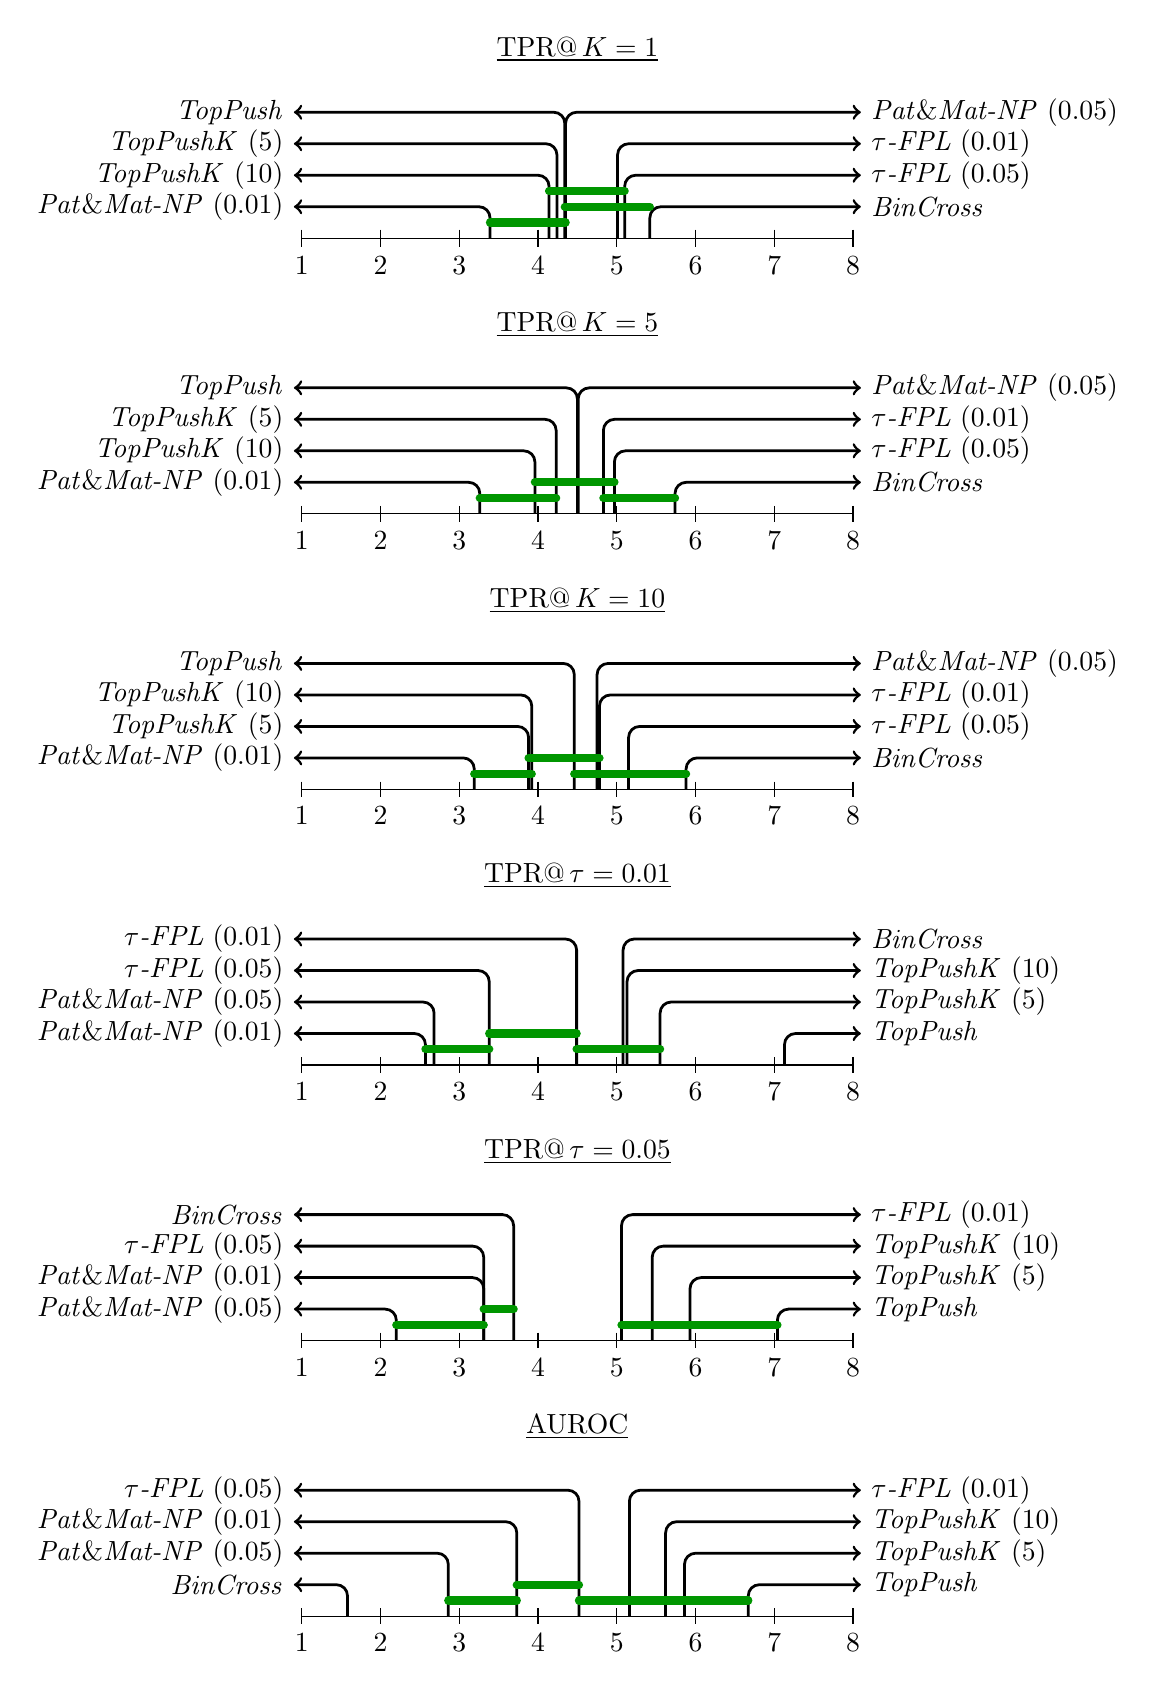
\begin{tikzpicture}  \node at (4.5,2.4) {\underline{$\auroc$}}; 
  \draw (1,0) -- (8,0); 
  \foreach \x in {1,...,8} \draw (\x,0.1) -- (\x,-0.1) node[anchor=north]{$\x$}; 
  \draw[line_node] (1.58,0) -- (1.58,0.4) -- (0.9, 0.4) node[anchor=east] {\BaseLine}; 
  \draw[line_node] (2.86,0) -- (2.86,0.8) -- (0.9, 0.8) node[anchor=east] {\PatMatNP(0.05)}; 
  \draw[line_node] (3.73,0) -- (3.73,1.2) -- (0.9, 1.2) node[anchor=east] {\PatMatNP(0.01)}; 
  \draw[line_node] (4.52,0) -- (4.52,1.6) -- (0.9, 1.6) node[anchor=east] {\tauFPL(0.05)}; 
  \draw[line_node] (5.16,0) -- (5.16,1.6) -- (8.1, 1.6) node[anchor=west] {\tauFPL(0.01)}; 
  \draw[line_node] (5.62,0) -- (5.62,1.2) -- (8.1, 1.2) node[anchor=west] {\TopPushK(10)}; 
  \draw[line_node] (5.86,0) -- (5.86,0.8) -- (8.1, 0.8) node[anchor=west] {\TopPushK(5)}; 
  \draw[line_node] (6.67,0) -- (6.67,0.4) -- (8.1, 0.4) node[anchor=west] {\TopPush}; 
  \draw[line_cv] (2.86,0.2) -- (3.73, 0.2); 
  \draw[line_cv] (3.73,0.4) -- (4.52, 0.4); 
  \draw[line_cv] (4.52,0.2) -- (5.62, 0.2); 
  \draw[line_cv] (5.16,0.2) -- (5.86, 0.2); 
  \draw[line_cv] (5.62,0.2) -- (6.67, 0.2); 


  \node at (4.5,5.9) {\underline{$\tpratfpr = 0.05$}}; 
  \draw (1,3.5) -- (8,3.5); 
  \foreach \x in {1,...,8} \draw (\x,3.6) -- (\x,3.4) node[anchor=north]{$\x$}; 
  \draw[line_node] (2.2,3.5) -- (2.2,3.9) -- (0.9, 3.9) node[anchor=east] {\PatMatNP(0.05)}; 
  \draw[line_node] (3.31,3.5) -- (3.31,4.3) -- (0.9, 4.3) node[anchor=east] {\PatMatNP(0.01)}; 
  \draw[line_node] (3.31,3.5) -- (3.31,4.7) -- (0.9, 4.7) node[anchor=east] {\tauFPL(0.05)}; 
  \draw[line_node] (3.69,3.5) -- (3.69,5.1) -- (0.9, 5.1) node[anchor=east] {\BaseLine}; 
  \draw[line_node] (5.06,3.5) -- (5.06,5.1) -- (8.1, 5.1) node[anchor=west] {\tauFPL(0.01)}; 
  \draw[line_node] (5.45,3.5) -- (5.45,4.7) -- (8.1, 4.7) node[anchor=west] {\TopPushK(10)}; 
  \draw[line_node] (5.93,3.5) -- (5.93,4.3) -- (8.1, 4.3) node[anchor=west] {\TopPushK(5)}; 
  \draw[line_node] (7.04,3.5) -- (7.04,3.9) -- (8.1, 3.9) node[anchor=west] {\TopPush}; 
  \draw[line_cv] (2.2,3.7) -- (3.31, 3.7); 
  \draw[line_cv] (3.31,3.9) -- (3.69, 3.9); 
  \draw[line_cv] (5.06,3.7) -- (5.93, 3.7); 
  \draw[line_cv] (5.93,3.7) -- (7.04, 3.7); 


  \node at (4.5,9.4) {\underline{$\tpratfpr = 0.01$}}; 
  \draw (1,7.0) -- (8,7.0); 
  \foreach \x in {1,...,8} \draw (\x,7.1) -- (\x,6.9) node[anchor=north]{$\x$}; 
  \draw[line_node] (2.57,7.0) -- (2.57,7.4) -- (0.9, 7.4) node[anchor=east] {\PatMatNP(0.01)}; 
  \draw[line_node] (2.68,7.0) -- (2.68,7.8) -- (0.9, 7.8) node[anchor=east] {\PatMatNP(0.05)}; 
  \draw[line_node] (3.38,7.0) -- (3.38,8.2) -- (0.9, 8.2) node[anchor=east] {\tauFPL(0.05)}; 
  \draw[line_node] (4.49,7.0) -- (4.49,8.6) -- (0.9, 8.6) node[anchor=east] {\tauFPL(0.01)}; 
  \draw[line_node] (5.08,7.0) -- (5.08,8.6) -- (8.1, 8.6) node[anchor=west] {\BaseLine}; 
  \draw[line_node] (5.13,7.0) -- (5.13,8.2) -- (8.1, 8.2) node[anchor=west] {\TopPushK(10)}; 
  \draw[line_node] (5.55,7.0) -- (5.55,7.8) -- (8.1, 7.8) node[anchor=west] {\TopPushK(5)}; 
  \draw[line_node] (7.13,7.0) -- (7.13,7.4) -- (8.1, 7.4) node[anchor=west] {\TopPush}; 
  \draw[line_cv] (2.57,7.2) -- (3.38, 7.2); 
  \draw[line_cv] (3.38,7.4) -- (4.49, 7.4); 
  \draw[line_cv] (4.49,7.2) -- (5.55, 7.2); 


  \node at (4.5,12.9) {\underline{$\tpratk =10$}}; 
  \draw (1,10.5) -- (8,10.5); 
  \foreach \x in {1,...,8} \draw (\x,10.6) -- (\x,10.4) node[anchor=north]{$\x$}; 
  \draw[line_node] (3.19,10.5) -- (3.19,10.9) -- (0.9, 10.9) node[anchor=east] {\PatMatNP(0.01)}; 
  \draw[line_node] (3.88,10.5) -- (3.88,11.3) -- (0.9, 11.3) node[anchor=east] {\TopPushK(5)}; 
  \draw[line_node] (3.92,10.5) -- (3.92,11.7) -- (0.9, 11.7) node[anchor=east] {\TopPushK(10)}; 
  \draw[line_node] (4.46,10.5) -- (4.46,12.1) -- (0.9, 12.1) node[anchor=east] {\TopPush}; 
  \draw[line_node] (4.75,10.5) -- (4.75,12.1) -- (8.1, 12.1) node[anchor=west] {\PatMatNP(0.05)}; 
  \draw[line_node] (4.78,10.5) -- (4.78,11.7) -- (8.1, 11.7) node[anchor=west] {\tauFPL(0.01)}; 
  \draw[line_node] (5.15,10.5) -- (5.15,11.3) -- (8.1, 11.3) node[anchor=west] {\tauFPL(0.05)}; 
  \draw[line_node] (5.88,10.5) -- (5.88,10.9) -- (8.1, 10.9) node[anchor=west] {\BaseLine}; 
  \draw[line_cv] (3.19,10.7) -- (3.92, 10.7); 
  \draw[line_cv] (3.88,10.9) -- (4.78, 10.9); 
  \draw[line_cv] (4.46,10.7) -- (5.15, 10.7); 
  \draw[line_cv] (4.75,10.7) -- (5.88, 10.7); 


  \node at (4.5,16.4) {\underline{$\tpratk =5$}}; 
  \draw (1,14.0) -- (8,14.0); 
  \foreach \x in {1,...,8} \draw (\x,14.1) -- (\x,13.9) node[anchor=north]{$\x$}; 
  \draw[line_node] (3.26,14.0) -- (3.26,14.4) -- (0.9, 14.4) node[anchor=east] {\PatMatNP(0.01)}; 
  \draw[line_node] (3.96,14.0) -- (3.96,14.8) -- (0.9, 14.8) node[anchor=east] {\TopPushK(10)}; 
  \draw[line_node] (4.23,14.0) -- (4.23,15.2) -- (0.9, 15.2) node[anchor=east] {\TopPushK(5)}; 
  \draw[line_node] (4.5,14.0) -- (4.5,15.6) -- (0.9, 15.6) node[anchor=east] {\TopPush}; 
  \draw[line_node] (4.51,14.0) -- (4.51,15.6) -- (8.1, 15.6) node[anchor=west] {\PatMatNP(0.05)}; 
  \draw[line_node] (4.83,14.0) -- (4.83,15.2) -- (8.1, 15.2) node[anchor=west] {\tauFPL(0.01)}; 
  \draw[line_node] (4.97,14.0) -- (4.97,14.8) -- (8.1, 14.8) node[anchor=west] {\tauFPL(0.05)}; 
  \draw[line_node] (5.74,14.0) -- (5.74,14.4) -- (8.1, 14.4) node[anchor=west] {\BaseLine}; 
  \draw[line_cv] (3.26,14.2) -- (4.23, 14.2); 
  \draw[line_cv] (3.96,14.4) -- (4.97, 14.4); 
  \draw[line_cv] (4.83,14.2) -- (5.74, 14.2); 


  \node at (4.5,19.9) {\underline{$\tpratk =1$}}; 
  \draw (1,17.5) -- (8,17.5); 
  \foreach \x in {1,...,8} \draw (\x,17.61) -- (\x,17.39) node[anchor=north]{$\x$}; 
  \draw[line_node] (3.39,17.5) -- (3.39,17.9) -- (0.9, 17.9) node[anchor=east] {\PatMatNP(0.01)}; 
  \draw[line_node] (4.14,17.5) -- (4.14,18.3) -- (0.9, 18.3) node[anchor=east] {\TopPushK(10)}; 
  \draw[line_node] (4.24,17.5) -- (4.24,18.7) -- (0.9, 18.7) node[anchor=east] {\TopPushK(5)}; 
  \draw[line_node] (4.34,17.5) -- (4.34,19.1) -- (0.9, 19.1) node[anchor=east] {\TopPush}; 
  \draw[line_node] (4.35,17.5) -- (4.35,19.1) -- (8.1, 19.1) node[anchor=west] {\PatMatNP(0.05)}; 
  \draw[line_node] (5.01,17.5) -- (5.01,18.7) -- (8.1, 18.7) node[anchor=west] {\tauFPL(0.01)}; 
  \draw[line_node] (5.1,17.5) -- (5.1,18.3) -- (8.1, 18.3) node[anchor=west] {\tauFPL(0.05)}; 
  \draw[line_node] (5.42,17.5) -- (5.42,17.9) -- (8.1, 17.9) node[anchor=west] {\BaseLine}; 
  \draw[line_cv] (3.39,17.7) -- (4.35, 17.7); 
  \draw[line_cv] (4.14,18.1) -- (5.1, 18.1); 
  \draw[line_cv] (4.34,17.9) -- (5.42, 17.9); 
\end{tikzpicture}

  \caption{\textbf{Primal formulation with linear model:} Critical difference (CD) diagrams (level of importance 0.05) of the Nemenyi post hoc test for the Friedman test. Each diagram shows the mean rank of each method, with rank 1 being the best. Green wide horizontal lines group together methods with the mean ranks that are not significantly different. The critical difference diagrams were computed for mean rank averages over all datasets.}
  \label{fig: critical diagrams primal}
\end{figure}

\newpage

\subsection{Dual Formulation: Linear Model}\label{sec: results dual}

\begin{table}[!p]
  \centering
  \underline{$\tpratk =10$}
  \vspace{0.25cm}\\
  \resizebox{\columnwidth}{!}{% 
    \begin{NiceTabular}{lcccccc}
      \CodeBefore
        \rowcolor{\headercol}{1}
        \rowcolors{3}{\rowcol}{}[restart]
      \Body
      \toprule
      \textbf{Formulation}
        & \textbf{MNIST}
        & \textbf{FashionMNIST}
        & \textbf{CIFAR10}
        & \textbf{CIFAR20}
        & \textbf{CIFAR100}
        & \textbf{SVHN2}\\
      \midrule
      \SVM
        & 97.89
        & \best{95.40}
        & 9.10
        & 4.90
        & \best{11.50}
        & 4.52 \\
      \TopPush
        & 97.62
        & 94.80
        & 10.45
        & \best{6.10}
        & 11.00
        & 5.23 \\
      \TopPushK(5)
        & 97.97
        & 94.90
        & 10.05
        & 6.00
        & 11.0
        & 5.07 \\
      \TopPushK(10)
        & 97.97
        & 94.90
        & 9.85
        & \best{6.10}
        & 11.00
        & 5.18 \\
      \tauFPL(0.01)
        & \best{98.02}
        & 95.05
        & \best{10.70}
        & 5.90
        & 10.5
        & \best{5.25} \\
      \tauFPL(0.05)
        & 92.56
        & \worst{92.20}
        & 10.15
        & 5.10
        & 10.0
        & 5.24 \\
      \PatMatNP(0.01)
        & 88.37
        & 92.50
        & \worst{7.45}
        & 1.40
        & \worst{5.00}
        & \worst{4.02} \\
      \PatMatNP(0.05)
        & \worst{52.60}
        & 92.50
        & \worst{7.45}
        & \worst{1.30}
        & \worst{5.00}
        & 4.05 \\
      \bottomrule
    \end{NiceTabular}
  }
  \vspace{0.25cm}\\
  \underline{$\tpratfpr = 0.05$}
  \vspace{0.25cm}\\
  \resizebox{\columnwidth}{!}{% 
    \begin{NiceTabular}{lcccccc}
      \CodeBefore
        \rowcolor{\headercol}{1}
        \rowcolors{3}{\rowcol}{}[restart]
      \Body
      \toprule
      \textbf{Formulation}
        & \textbf{MNIST}
        & \textbf{FashionMNIST}
        & \textbf{CIFAR10}
        & \textbf{CIFAR20}
        & \textbf{CIFAR100}
        & \textbf{SVHN2}\\
      \midrule
      \SVM
        & 99.74
        & 98.90
        & 60.00
        & \best{44.80}
        & 59.00
        & \worst{59.72} \\
      \TopPush
        & 99.74
        & 98.80
        & 57.10
        & \worst{37.70}
        & 59.50
        & 72.54 \\
      \TopPushK(5)
        & \best{99.82}
        & 98.90
        & 56.25
        & 38.80
        & \worst{57.50}
        & 71.40 \\
      \TopPushK(10)
        & \best{99.82}
        & 98.90
        & 56.90
        & 38.70
        & 58.00
        & 71.61 \\
      \tauFPL(0.01)
        & \best{99.82}
        & 98.90
        & 58.10
        & 39.10
        & 59.00
        & 73.52 \\
      \tauFPL(0.05)
        & 99.74
        & \best{99.10}
        & \best{60.80}
        & 44.40
        & 61.00
        & \best{74.26} \\
      \PatMatNP(0.01)
        & \worst{99.30}
        & \worst{98.10}
        & \worst{54.70}
        & 44.60
        & 62.50
        & 63.47 \\
      \PatMatNP(0.05)
        & 99.38
        & \worst{98.10}
        & \worst{54.70}
        & 44.50
        & \best{63.50}
        & 63.48 \\
      \bottomrule
    \end{NiceTabular}
  }
  \vspace{0.25cm}\\
  \underline{$\auroc$}
  \vspace{0.25cm}\\
  \resizebox{\columnwidth}{!}{% 
    \begin{NiceTabular}{lcccccc}
      \CodeBefore
        \rowcolor{\headercol}{1}
        \rowcolors{3}{\rowcol}{}[restart]
      \Body
      \toprule
      \textbf{Formulation}
        & \textbf{MNIST}
        & \textbf{FashionMNIST}
        & \textbf{CIFAR10}
        & \textbf{CIFAR20}
        & \textbf{CIFAR100}
        & \textbf{SVHN2}\\
      \midrule
      \SVM
        & 99.94
        & 99.66
        & 90.02
        & 79.75
        & 87.80
        & \worst{90.14} \\
      \TopPush
        & 99.94
        & 99.56
        & 89.35
        & 79.06
        & \worst{87.03}
        & 92.77 \\
      \TopPushK(5)
        & 99.95
        & 99.64
        & 89.05
        & 79.13
        & 87.21
        & 92.60 \\
      \TopPushK(10)
        & 99.95
        & 99.67
        & 89.16
        & 79.27
        & 87.78
        & 92.67 \\
      \tauFPL(0.01)
        & \best{99.97}
        & 99.68
        & 89.83
        & 79.07
        & 87.64
        & 92.98 \\
      \tauFPL(0.05)
        & 99.93
        & \best{99.80}
        & \best{90.34}
        & \best{80.17}
        & 88.56
        & \best{93.16} \\
      \PatMatNP(0.01)
        & \worst{99.78}
        & \worst{99.40}
        & 87.62
        & 78.82
        & \best{89.78}
        & 90.80 \\
      \PatMatNP(0.05)
        & \worst{99.78}
        & \worst{99.40}
        & \worst{87.61}
        & \worst{78.76}
        & 89.52
        & 90.82 \\
      \bottomrule
    \end{NiceTabular}
  }
  \caption{\textbf{Dual formulations with gaussian kernel:} Each table corresponds to one performance metric and all presented results are medians of ten independent runs for each pair of datasets and formulation. The best result for each dataset is highlighted in green, while the worst result is highlighted in red.}
  \label{tab: dual auc}
\end{table}

\begin{figure}[!p]
  \centering
  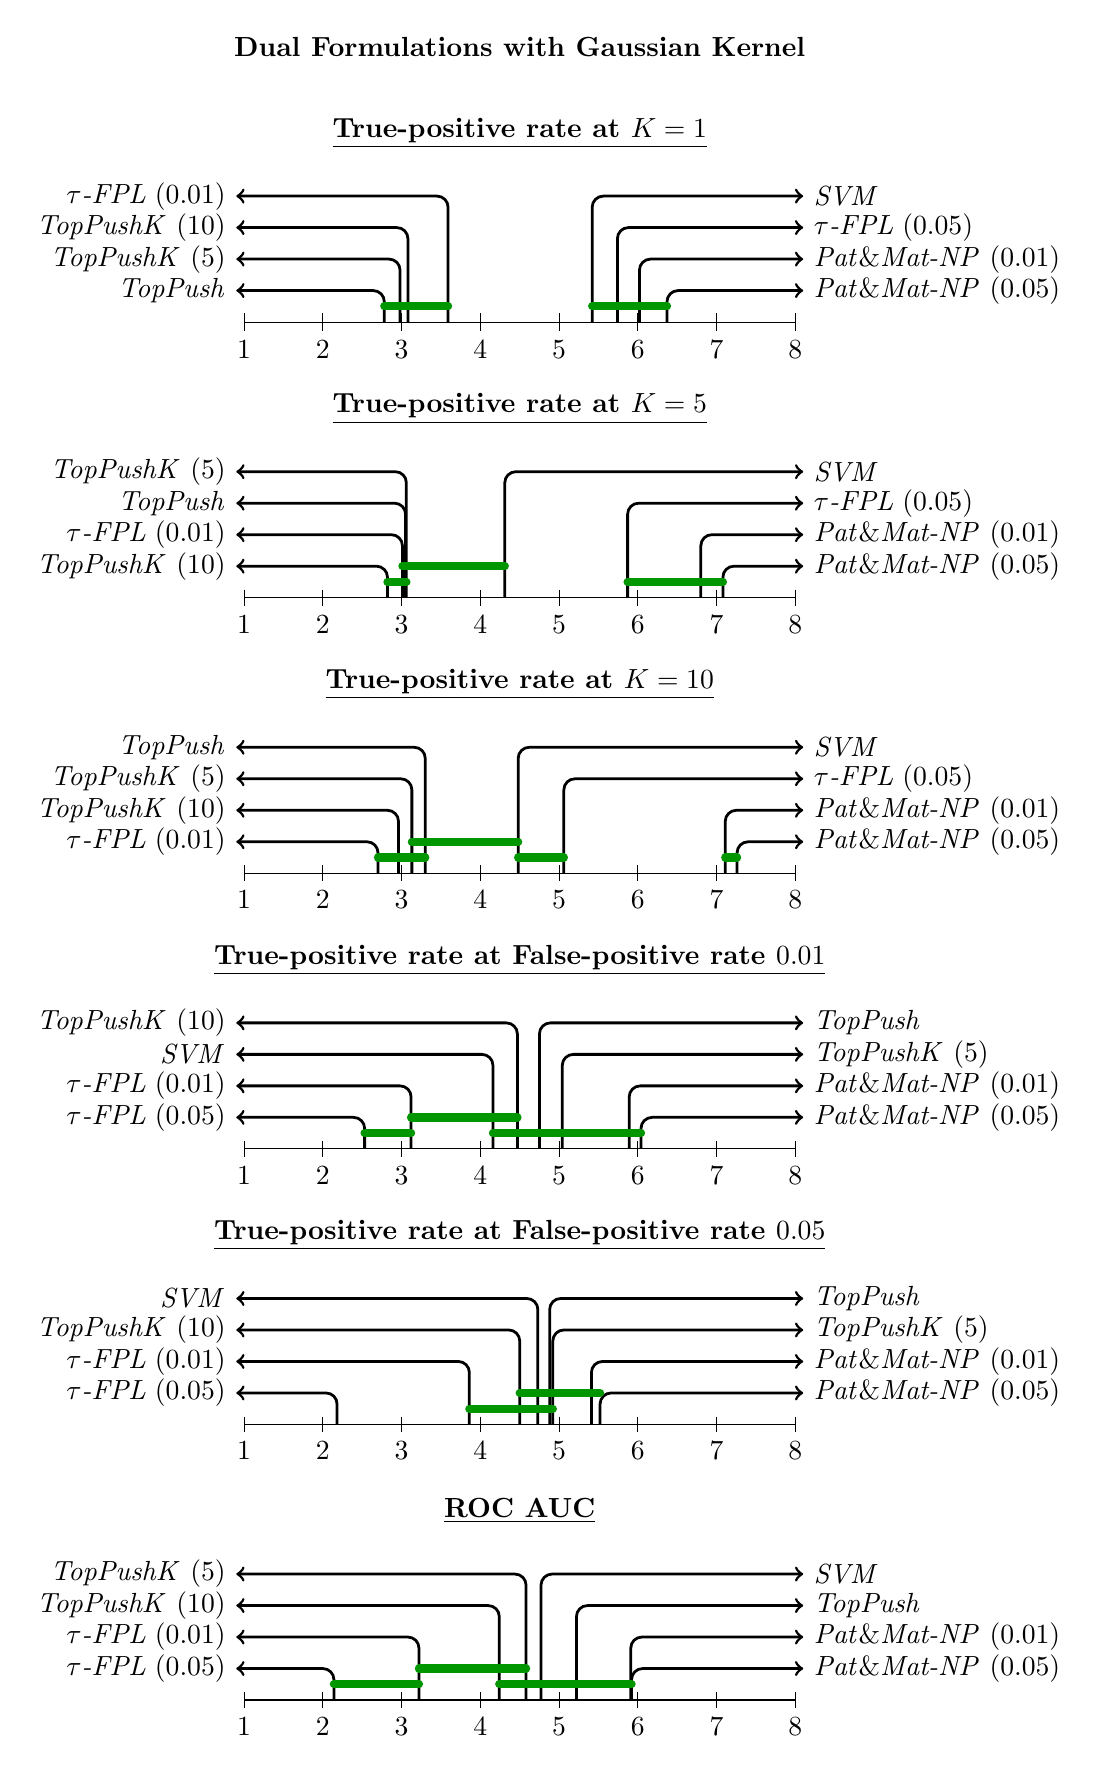
\begin{tikzpicture}  \node at (4.5,2.4) {\textbf{\underline{ROC AUC}}}; 
  \draw (1,0) -- (8,0); 
  \foreach \x in {1,...,8} \draw (\x,0.1) -- (\x,-0.1) node[anchor=north]{$\x$}; 
  \draw[line_node] (2.14,0) -- (2.14,0.4) -- (0.9, 0.4) node[anchor=east] {\tauFPL(0.05)}; 
  \draw[line_node] (3.22,0) -- (3.22,0.8) -- (0.9, 0.8) node[anchor=east] {\tauFPL(0.01)}; 
  \draw[line_node] (4.24,0) -- (4.24,1.2) -- (0.9, 1.2) node[anchor=east] {\TopPushK(10)}; 
  \draw[line_node] (4.58,0) -- (4.58,1.6) -- (0.9, 1.6) node[anchor=east] {\TopPushK(5)}; 
  \draw[line_node] (4.77,0) -- (4.77,1.6) -- (8.1, 1.6) node[anchor=west] {\SVM}; 
  \draw[line_node] (5.22,0) -- (5.22,1.2) -- (8.1, 1.2) node[anchor=west] {\TopPush}; 
  \draw[line_node] (5.91,0) -- (5.91,0.8) -- (8.1, 0.8) node[anchor=west] {\PatMatNP(0.01)}; 
  \draw[line_node] (5.92,0) -- (5.92,0.4) -- (8.1, 0.4) node[anchor=west] {\PatMatNP(0.05)}; 
  \draw[line_cv] (2.14,0.2) -- (3.22, 0.2); 
  \draw[line_cv] (3.22,0.4) -- (4.58, 0.4); 
  \draw[line_cv] (4.24,0.2) -- (5.22, 0.2); 
  \draw[line_cv] (4.58,0.2) -- (5.92, 0.2); 


  \node at (4.5,5.9) {\textbf{\underline{True-positive rate at False-positive rate $0.05$}}}; 
  \draw (1,3.5) -- (8,3.5); 
  \foreach \x in {1,...,8} \draw (\x,3.6) -- (\x,3.4) node[anchor=north]{$\x$}; 
  \draw[line_node] (2.18,3.5) -- (2.18,3.9) -- (0.9, 3.9) node[anchor=east] {\tauFPL(0.05)}; 
  \draw[line_node] (3.86,3.5) -- (3.86,4.3) -- (0.9, 4.3) node[anchor=east] {\tauFPL(0.01)}; 
  \draw[line_node] (4.5,3.5) -- (4.5,4.7) -- (0.9, 4.7) node[anchor=east] {\TopPushK(10)}; 
  \draw[line_node] (4.73,3.5) -- (4.73,5.1) -- (0.9, 5.1) node[anchor=east] {\SVM}; 
  \draw[line_node] (4.88,3.5) -- (4.88,5.1) -- (8.1, 5.1) node[anchor=west] {\TopPush}; 
  \draw[line_node] (4.92,3.5) -- (4.92,4.7) -- (8.1, 4.7) node[anchor=west] {\TopPushK(5)}; 
  \draw[line_node] (5.41,3.5) -- (5.41,4.3) -- (8.1, 4.3) node[anchor=west] {\PatMatNP(0.01)}; 
  \draw[line_node] (5.52,3.5) -- (5.52,3.9) -- (8.1, 3.9) node[anchor=west] {\PatMatNP(0.05)}; 
  \draw[line_cv] (3.86,3.7) -- (4.92, 3.7); 
  \draw[line_cv] (4.5,3.9) -- (5.52, 3.9); 


  \node at (4.5,9.4) {\textbf{\underline{True-positive rate at False-positive rate $0.01$}}}; 
  \draw (1,7.0) -- (8,7.0); 
  \foreach \x in {1,...,8} \draw (\x,7.1) -- (\x,6.9) node[anchor=north]{$\x$}; 
  \draw[line_node] (2.53,7.0) -- (2.53,7.4) -- (0.9, 7.4) node[anchor=east] {\tauFPL(0.05)}; 
  \draw[line_node] (3.12,7.0) -- (3.12,7.8) -- (0.9, 7.8) node[anchor=east] {\tauFPL(0.01)}; 
  \draw[line_node] (4.16,7.0) -- (4.16,8.2) -- (0.9, 8.2) node[anchor=east] {\SVM}; 
  \draw[line_node] (4.47,7.0) -- (4.47,8.6) -- (0.9, 8.6) node[anchor=east] {\TopPushK(10)}; 
  \draw[line_node] (4.75,7.0) -- (4.75,8.6) -- (8.1, 8.6) node[anchor=west] {\TopPush}; 
  \draw[line_node] (5.04,7.0) -- (5.04,8.2) -- (8.1, 8.2) node[anchor=west] {\TopPushK(5)}; 
  \draw[line_node] (5.89,7.0) -- (5.89,7.8) -- (8.1, 7.8) node[anchor=west] {\PatMatNP(0.01)}; 
  \draw[line_node] (6.04,7.0) -- (6.04,7.4) -- (8.1, 7.4) node[anchor=west] {\PatMatNP(0.05)}; 
  \draw[line_cv] (2.53,7.2) -- (3.12, 7.2); 
  \draw[line_cv] (3.12,7.4) -- (4.47, 7.4); 
  \draw[line_cv] (4.16,7.2) -- (5.04, 7.2); 
  \draw[line_cv] (4.75,7.2) -- (6.04, 7.2); 


  \node at (4.5,12.9) {\textbf{\underline{True-positive rate at $K = 10$}}}; 
  \draw (1,10.5) -- (8,10.5); 
  \foreach \x in {1,...,8} \draw (\x,10.6) -- (\x,10.4) node[anchor=north]{$\x$}; 
  \draw[line_node] (2.7,10.5) -- (2.7,10.9) -- (0.9, 10.9) node[anchor=east] {\tauFPL(0.01)}; 
  \draw[line_node] (2.96,10.5) -- (2.96,11.3) -- (0.9, 11.3) node[anchor=east] {\TopPushK(10)}; 
  \draw[line_node] (3.13,10.5) -- (3.13,11.7) -- (0.9, 11.7) node[anchor=east] {\TopPushK(5)}; 
  \draw[line_node] (3.3,10.5) -- (3.3,12.1) -- (0.9, 12.1) node[anchor=east] {\TopPush}; 
  \draw[line_node] (4.48,10.5) -- (4.48,12.1) -- (8.1, 12.1) node[anchor=west] {\SVM}; 
  \draw[line_node] (5.06,10.5) -- (5.06,11.7) -- (8.1, 11.7) node[anchor=west] {\tauFPL(0.05)}; 
  \draw[line_node] (7.11,10.5) -- (7.11,11.3) -- (8.1, 11.3) node[anchor=west] {\PatMatNP(0.01)}; 
  \draw[line_node] (7.26,10.5) -- (7.26,10.9) -- (8.1, 10.9) node[anchor=west] {\PatMatNP(0.05)}; 
  \draw[line_cv] (2.7,10.7) -- (3.3, 10.7); 
  \draw[line_cv] (3.13,10.9) -- (4.48, 10.9); 
  \draw[line_cv] (4.48,10.7) -- (5.06, 10.7); 
  \draw[line_cv] (7.11,10.7) -- (7.26, 10.7); 


  \node at (4.5,16.4) {\textbf{\underline{True-positive rate at $K = 5$}}}; 
  \draw (1,14.0) -- (8,14.0); 
  \foreach \x in {1,...,8} \draw (\x,14.1) -- (\x,13.9) node[anchor=north]{$\x$}; 
  \draw[line_node] (2.82,14.0) -- (2.82,14.4) -- (0.9, 14.4) node[anchor=east] {\TopPushK(10)}; 
  \draw[line_node] (3.01,14.0) -- (3.01,14.8) -- (0.9, 14.8) node[anchor=east] {\tauFPL(0.01)}; 
  \draw[line_node] (3.05,14.0) -- (3.05,15.2) -- (0.9, 15.2) node[anchor=east] {\TopPush}; 
  \draw[line_node] (3.06,14.0) -- (3.06,15.6) -- (0.9, 15.6) node[anchor=east] {\TopPushK(5)}; 
  \draw[line_node] (4.31,14.0) -- (4.31,15.6) -- (8.1, 15.6) node[anchor=west] {\SVM}; 
  \draw[line_node] (5.87,14.0) -- (5.87,15.2) -- (8.1, 15.2) node[anchor=west] {\tauFPL(0.05)}; 
  \draw[line_node] (6.8,14.0) -- (6.8,14.8) -- (8.1, 14.8) node[anchor=west] {\PatMatNP(0.01)}; 
  \draw[line_node] (7.08,14.0) -- (7.08,14.4) -- (8.1, 14.4) node[anchor=west] {\PatMatNP(0.05)}; 
  \draw[line_cv] (2.82,14.2) -- (3.06, 14.2); 
  \draw[line_cv] (3.01,14.4) -- (4.31, 14.4); 
  \draw[line_cv] (5.87,14.2) -- (7.08, 14.2); 


  \node at (4.5,19.9) {\textbf{\underline{True-positive rate at $K = 1$}}}; 
  \draw (1,17.5) -- (8,17.5); 
  \foreach \x in {1,...,8} \draw (\x,17.61) -- (\x,17.39) node[anchor=north]{$\x$}; 
  \draw[line_node] (2.78,17.5) -- (2.78,17.9) -- (0.9, 17.9) node[anchor=east] {\TopPush}; 
  \draw[line_node] (2.98,17.5) -- (2.98,18.3) -- (0.9, 18.3) node[anchor=east] {\TopPushK(5)}; 
  \draw[line_node] (3.08,17.5) -- (3.08,18.7) -- (0.9, 18.7) node[anchor=east] {\TopPushK(10)}; 
  \draw[line_node] (3.59,17.5) -- (3.59,19.1) -- (0.9, 19.1) node[anchor=east] {\tauFPL(0.01)}; 
  \draw[line_node] (5.42,17.5) -- (5.42,19.1) -- (8.1, 19.1) node[anchor=west] {\SVM}; 
  \draw[line_node] (5.74,17.5) -- (5.74,18.7) -- (8.1, 18.7) node[anchor=west] {\tauFPL(0.05)}; 
  \draw[line_node] (6.02,17.5) -- (6.02,18.3) -- (8.1, 18.3) node[anchor=west] {\PatMatNP(0.01)}; 
  \draw[line_node] (6.37,17.5) -- (6.37,17.9) -- (8.1, 17.9) node[anchor=west] {\PatMatNP(0.05)}; 
  \draw[line_cv] (2.78,17.7) -- (3.59, 17.7); 
  \draw[line_cv] (5.42,17.7) -- (6.37, 17.7); 


\node at (4.5, 21.0) {\textbf{Dual Formulations with Gaussian Kernel}}; 
\end{tikzpicture}

  \caption{\textbf{Dual formulations with gaussian kernel:} Critical difference (CD) diagrams (level of importance 0.05) of the Nemenyi post hoc test for the Friedman test. Each diagram shows the mean rank of each method, with rank 1 being the best. Green wide horizontal lines group together methods with the mean ranks that are not significantly different. The critical difference diagrams were computed for mean rank averages over all datasets.}
  \label{fig: critical diagrams dual gauss}
\end{figure}

\newpage

\subsection{Primal Formulation: Non-Linear Model}\label{sec: results primal nonlinear}

In this subsection, we discuss result for the case of primal formulations with linear model, i.e. resutls presented here are related to the Chapter~\ref{chap: linear}.

\begin{table}[!p]
  \centering
  \underline{$\tpratk =10$}
  \vspace{0.25cm}\\
  \resizebox{\columnwidth}{!}{% 
    \begin{NiceTabular}{lccccccc}
      \CodeBefore
        \rowcolor{\headercol}{1}
        \rowcolors{3}{\rowcol}{}[restart]
      \Body
      \toprule
      \textbf{Formulation}
        & \textbf{MNIST}
        & \textbf{FashionMNIST}
        & \textbf{CIFAR10}
        & \textbf{CIFAR20}
        & \textbf{CIFAR100}
        & \textbf{SVHN2}
        & \textbf{SVHN2Extra}\\
      \midrule
      \BaseLine
        & \best{99.26}
        & \best{98.10}
        & 11.40
        & 3.50
        & 5.00
        & 11.34
        & 15.95 \\
      \DeepTopPush
        & 98.42
        & 97.60
        & \worst{0.20}
        & 0.20
        & \worst{0.00}
        & \worst{0.17}
        & \worst{0.00} \\
      \TopPushK(5)
        & 98.54
        & 97.50
        & 2.00
        & \worst{0.00}
        & 8.50
        & 10.58
        & 16.12 \\
      \TopPushK(10)
        & 98.24
        & 96.90
        & 12.55
        & \best{100.00}
        & \best{100.00}
        & \best{100.00}
        & \best{100.00} \\
      \tauFPL(0.01)
        & 98.72
        & 97.50
        & 1.00
        & 0.20
        & 9.00
        & 9.52
        & \worst{0.00} \\
      \tauFPL(0.05)
        & 96.78
        & 96.50
        & 14.80
        & 0.30
        & 8.50
        & 13.05
        & 12.48 \\
      \PatMatNP(0.01)
        & 98.54
        & 97.45
        & \best{32.45}
        & 4.80
        & 20.00
        & 13.92
        & 19.33 \\
      \PatMatNP(0.05)
        & \worst{82.86}
        & \worst{94.30}
        & 26.55
        & 5.90
        & 11.50
        & 11.36
        & 15.98 \\
      \bottomrule
    \end{NiceTabular}
  }
  \vspace{0.25cm}\\
  \underline{$\tpratfpr = 0.05$}
  \vspace{0.25cm}\\
  \resizebox{\columnwidth}{!}{% 
    \begin{NiceTabular}{lccccccc}
      \CodeBefore
        \rowcolor{\headercol}{1}
        \rowcolors{3}{\rowcol}{}[restart]
      \Body
      \toprule
      \textbf{Formulation}
        & \textbf{MNIST}
        & \textbf{FashionMNIST}
        & \textbf{CIFAR10}
        & \textbf{CIFAR20}
        & \textbf{CIFAR100}
        & \textbf{SVHN2}
        & \textbf{SVHN2Extra}\\
      \midrule
      \BaseLine
        & \best{100.00}
        & \best{99.90}
        & 83.35
        & 48.00
        & 82.00
        & 94.66
        & 97.71 \\
      \DeepTopPush
        & \worst{99.82}
        & \worst{99.70}
        & \worst{5.85}
        & 8.90
        & 9.00
        & 40.14
        & \worst{0.00} \\
      \TopPushK(5)
        & \best{100.00}
        & 99.85
        & 34.30
        & 7.70
        & 53.50
        & 86.54
        & 93.96 \\
      \TopPushK(10)
        & \best{100.00}
        & \best{99.90}
        & 27.95
        & \worst{0.00}
        & \worst{0.00}
        & \worst{0.00}
        & \worst{0.00} \\
      \tauFPL(0.01)
        & \best{100.00}
        & \best{99.90}
        & 24.40
        & 11.50
        & 65.50
        & 87.60
        & \worst{0.00} \\
      \tauFPL(0.05)
        & \best{100.00}
        & \best{99.90}
        & 82.75
        & 18.00
        & 66.50
        & 94.51
        & 97.52 \\
      \PatMatNP(0.01)
        & \best{100.00}
        & \best{99.90}
        & 91.55
        & 52.20
        & 79.00
        & 95.49
        & 98.43 \\
      \PatMatNP(0.05)
        & \best{100.00}
        & \best{99.90}
        & \best{91.75}
        & \best{57.70}
        & \best{85.00}
        & \best{95.53}
        & \best{98.50} \\
      \bottomrule
    \end{NiceTabular}
  }
  \vspace{0.25cm}\\
  \underline{$\auroc$}
  \vspace{0.25cm}\\
  \resizebox{\columnwidth}{!}{% 
    \begin{NiceTabular}{lccccccc}
      \CodeBefore
        \rowcolor{\headercol}{1}
        \rowcolors{3}{\rowcol}{}[restart]
      \Body
      \toprule
      \textbf{Formulation}
        & \textbf{MNIST}
        & \textbf{FashionMNIST}
        & \textbf{CIFAR10}
        & \textbf{CIFAR20}
        & \textbf{CIFAR100}
        & \textbf{SVHN2}
        & \textbf{SVHN2Extra}\\
      \midrule
      \BaseLine
        & \best{100.00}
        & \best{99.98}
        & 96.85
        & 84.67
        & 95.94
        & 98.54
        & 99.20 \\
      \DeepTopPush
        & 99.98
        & \worst{99.95}
        & \worst{49.51}
        & 59.40
        & 56.68
        & 83.12
        & 1.61 \\
      \TopPushK(5)
        & \best{100.0}
        & 99.97
        & 77.10
        & 55.50
        & 84.24
        & 96.57
        & 98.32 \\
      \TopPushK(10)
        & \best{100.00}
        & \best{99.98}
        & 74.26
        & \worst{0.00}
        & \worst{0.00}
        & \worst{0.00}
        & \worst{0.00} \\
      \tauFPL(0.01)
        & \best{100.0}
        & \best{99.98}
        & 70.96
        & 60.03
        & 90.16
        & 96.68
        & 25.84 \\
      \tauFPL(0.05)
        & 99.99
        & 99.97
        & 95.86
        & 68.18
        & 90.76
        & 98.50
        & 99.12 \\
      \PatMatNP(0.01)
        & 99.99
        & \best{99.98}
        & 97.90
        & 84.38
        & 93.84
        & 98.74
        & \best{99.38} \\
      \PatMatNP(0.05)
        & \worst{99.96}
        & 99.96
        & \best{98.24}
        & \best{88.39}
        & \best{96.56}
        & \best{98.76}
        & 99.32 \\
      \bottomrule
    \end{NiceTabular}
  }
  \caption{\textbf{Primal formulations with non-linear model:} Each table corresponds to one performance metric and all presented results are medians of ten independent runs for each pair of datasets and formulation. The best result for each dataset is highlighted in green, while the worst result is highlighted in red.}
  \label{tab: primalnn auc}
\end{table}

\begin{figure}[!p]
  \centering
  \documentclass{standalone}
% ------------------------------------------------------------------------------
% Packages
% ------------------------------------------------------------------------------
\usepackage[ddmmyyyy]{datetime}
\usepackage[T1]{fontenc}
\usepackage[utf8]{inputenc}

% Page setting
\usepackage[explicit]{titlesec}
\usepackage{sectsty}
\usepackage{fancyhdr}
\usepackage[title, titletoc]{appendix}

% Fonts
\usepackage{kpfonts}
\usepackage{amsmath}
\usepackage{amssymb}
\usepackage{dsfont}
\usepackage{pifont}

% Graphics and colors
\usepackage{graphicx}
\usepackage{xcolor}
\usepackage{import}

\definecolor{myred}{RGB}{150,0,0}
\definecolor{mygreen}{RGB}{0,150,0}
\definecolor{myblue}{RGB}{0, 101, 189}
\definecolor{myyellow}{RGB}{220, 206, 0}
\definecolor{myorange}{RGB}{255, 153, 51}
\definecolor{mycyan}{RGB}{51, 204, 204}
\definecolor{mypurple}{RGB}{204, 0, 153}

\newcommand{\doccol}{\color{myblue}}

% Hyperrefs
\usepackage[
  pdfusetitle,
  unicode = true,
  bookmarks = true,
  bookmarksnumbered = false,
  bookmarksopen = true,
  breaklinks = false,
  pdfborderstyle = {},
  backref = false,
  colorlinks = true,
  linkcolor = myblue,
  urlcolor = myred,
  citecolor = mygreen,
]{hyperref}


% Captions
\usepackage{caption}

\captionsetup[figure]{position = bottom}
\captionsetup[table]{position = bottom}

% Tables, Algs ...
\usepackage{enumitem}
\usepackage{algorithm}
\usepackage{algorithmicx}
\usepackage{algpseudocode}
\usepackage{booktabs}
\usepackage{nicematrix}

\renewcommand{\arraystretch}{1.5}

\newcommand{\headercol}{myblue!20}
\newcommand{\rowcol}{myblue!10}

% Math
\usepackage{nicefrac}
\usepackage{bm}
\usepackage{thm-restate}
\usepackage{optidef}
\usepackage{xspace}

% Theorems
\usepackage[framemethod=TikZ]{mdframed}
\usepackage{amsthm}
\usepackage{xifthen}

% Tikz and pfgplots
\usepackage{tikz}
\usepackage{pgfplots}
\usepackage{pgfplotstable}

\usetikzlibrary{shapes}
\usetikzlibrary{arrows}
\usetikzlibrary{automata}
\usetikzlibrary{positioning}
\usetikzlibrary{calc}
\usetikzlibrary{intersections}

\pgfplotsset{compat=newest}
\usepgfplotslibrary{groupplots}
\usepgfplotslibrary{fillbetween}

\tikzstyle{line_node} = [line width=1pt, rounded corners, color=black, ->]
\tikzstyle{line_cv} = [line width=3pt, color=mygreen, line cap=round]

% Tmp
\usepackage[color=myred!50]{todonotes}

% ------------------------------------------------------------------------------
% Math declarations
% ------------------------------------------------------------------------------
\newcommand{\Brac}[2][r]{%
  \ifx r#1 \left(       #2 \right)       \else
  \ifx c#1 \left\{      #2 \right\}      \else
  \ifx s#1 \left[       #2 \right]       \else
  \ifx v#1 \left\vert   #2 \right\vert   \else
  \ifx a#1 \left\langle #2 \right\rangle \else
  \ifx t#1 \left\lceil  #2 \right\rceil  \else
  \ifx b#1 \left\lfloor #2 \right\rfloor \else
  \ifx n#1 \left\|      #2 \right\|      \else
  \mathrm{Illegal~option}%
  \fi\fi\fi\fi\fi\fi\fi\fi
}

\newcommand{\clip}[4][s]{
  \ifx s#1 \mathrm{clip}_{\Brac[s]{#2,\; #3}}\Brac{#4} \else
  \ifx u#1 \mathrm{clip}_{\left[#2,\; #3\right)}\Brac{#4} \else
  \ifx l#1 \mathrm{clip}_{\left(#2,\; #3\right]}\Brac{#4} \else
  \mathrm{Illegal~option}%
  \fi\fi\fi
}

\DeclareMathOperator*{\argmax}{arg\,max}

\newcommand{\yesmark}{\textcolor{mygreen}{\ding{51}}}%
\newcommand{\nomark}{\textcolor{myred}{\ding{55}}}
\newcommand{\good}[1]{\textcolor{mygreen}{#1}}
\newcommand{\bad}[1]{\textcolor{myred}{#1}}

\newcommand{\R}{\mathbb{R}}
\newcommand{\N}{\mathbb{N}}
\newcommand{\X}{\mathbb{X}}

\newcommand{\I}{\mathcal{I}}
\newcommand{\Itil}{\tilde{\mathcal{I}}}
\newcommand{\Ineg}{\I_{-}}
\newcommand{\Ipos}{\I_{+}}

\newcommand{\Imb}{\I_{\text{mb}}}
\newcommand{\Imbneg}{\I_{\text{mb},-}}
\newcommand{\Imbpos}{\I_{\text{mb},+}}

\newcommand{\indmax}{j^{\star}}
\newcommand{\indmaxmb}{j^{\star}_{\text{mb}}}

\newcommand{\nall}{n}
\newcommand{\nneg}{n_{-}}
\newcommand{\npos}{n_{+}}
\newcommand{\ntil}{\tilde{n}}

\newcommand{\nmb}{n_{\text{mb}}}
\newcommand{\nmbneg}{n_{\text{mb},-}}
\newcommand{\nmbpos}{n_{\text{mb},+}}

\newcommand{\K}{\mathbb{K}}
\newcommand{\Kall}{\K^{\pm}}
\newcommand{\Kneg}{\K^{-}}

\newcommand{\alphak}{\alpha_{\hat{k}}}
\newcommand{\alphal}{\alpha_{\hat{l}}}
\newcommand{\betak}{\beta_{\hat{k}}}
\newcommand{\betal}{\beta_{\hat{l}}}

\newcommand{\norm}[1]{\Brac[n]{#1}}
\newcommand{\abs}[1]{|#1|}
\newcommand{\inner}[2]{\Brac[a]{#1, \; #2}}
\newcommand{\dd}[1]{\mathop{}\!\mathrm{d}#1}

\newcommand{\Iverson}[1]{\mathds{1}_{\Brac[s]{#1}}}

\newcommand{\EE}{\mathbb{E}}
\newcommand{\PP}{\mathbb{P}}
\newcommand{\bias}{\operatorname{bias}}

\newcommand{\Matrix}[1]{\begin{pmatrix} #1 \end{pmatrix}}
\newcommand{\Set}[2]{\Brac[c]{#1 \; \middle\vert \; #2}}
\newcommand{\domain}{\operatorname*{dom}}

\newcommand{\repeatloop}{\texttt{repeat}\xspace}
\newcommand{\forloop}{\texttt{for}\xspace}

\newcommand{\vecab}{\Matrix{\bm{\alpha} \\ \bm{\beta}}}

% models
\newcommand{\AccatTop}{\emph{Accuracy at the Top}\xspace}
\newcommand{\TopPush}{\emph{TopPush}\xspace}
\newcommand{\TopPushK}{\emph{TopPushK}\xspace}
\newcommand{\tauFPL}{{\emph{$\tau$-FPL}}\xspace}
\newcommand{\TopMeanK}{\emph{TopMeanK}\xspace}
\newcommand{\PatMat}{\emph{Pat}\&\emph{Mat}\xspace}
\newcommand{\PatMatNP}{{\emph{Pat}\&\emph{Mat-NP}}\xspace}
\newcommand{\Grill}{\emph{Grill}\xspace}
\newcommand{\GrillNP}{\emph{Grill-NP}\xspace}
\newcommand{\DeepTopPush}{\emph{DeepTopPush}\xspace}
\newcommand{\TFCO}{\emph{TFCO}\xspace}
\newcommand{\APPerf}{\emph{Ap-Perf}\xspace}
\newcommand{\BaseLine}{\emph{BinCross}\xspace}
\newcommand{\SVM}{\emph{SVM}\xspace}

% counts and rates
\DeclareMathOperator{\tp}{tp}
\DeclareMathOperator{\tn}{tn}
\DeclareMathOperator{\fp}{fp}
\DeclareMathOperator{\fn}{fn}
\DeclareMathOperator{\tpr}{tpr}
\DeclareMathOperator{\tnr}{tnr}
\DeclareMathOperator{\fpr}{fpr}
\DeclareMathOperator{\fnr}{fnr}

\DeclareMathOperator{\tps}{\overline{tp}}
\DeclareMathOperator{\tns}{\overline{tn}}
\DeclareMathOperator{\fps}{\overline{fp}}
\DeclareMathOperator{\fns}{\overline{fn}}

\DeclareMathOperator{\accuracy}{acc}
\DeclareMathOperator{\baccuracy}{bacc}
\DeclareMathOperator{\precision}{precision}
\DeclareMathOperator{\recall}{recall}
\DeclareMathOperator{\pratrec}{Precision@Recall}
\DeclareMathOperator{\postop}{pos@top}

\newcommand{\tpratk}{\operatorname{TPR@}K}
\newcommand{\tpratfpr}{\operatorname{TPR@}\tau}
\newcommand{\auroc}{\operatorname{AUROC}}


% ------------------------------------------------------------------------------
% Document
% ------------------------------------------------------------------------------
\tikzstyle{line_node} = [line width=1pt, rounded corners, color=black, ->]
\tikzstyle{line_cv} = [line width=3pt, color=mygreen, line cap=round]

\begin{document}
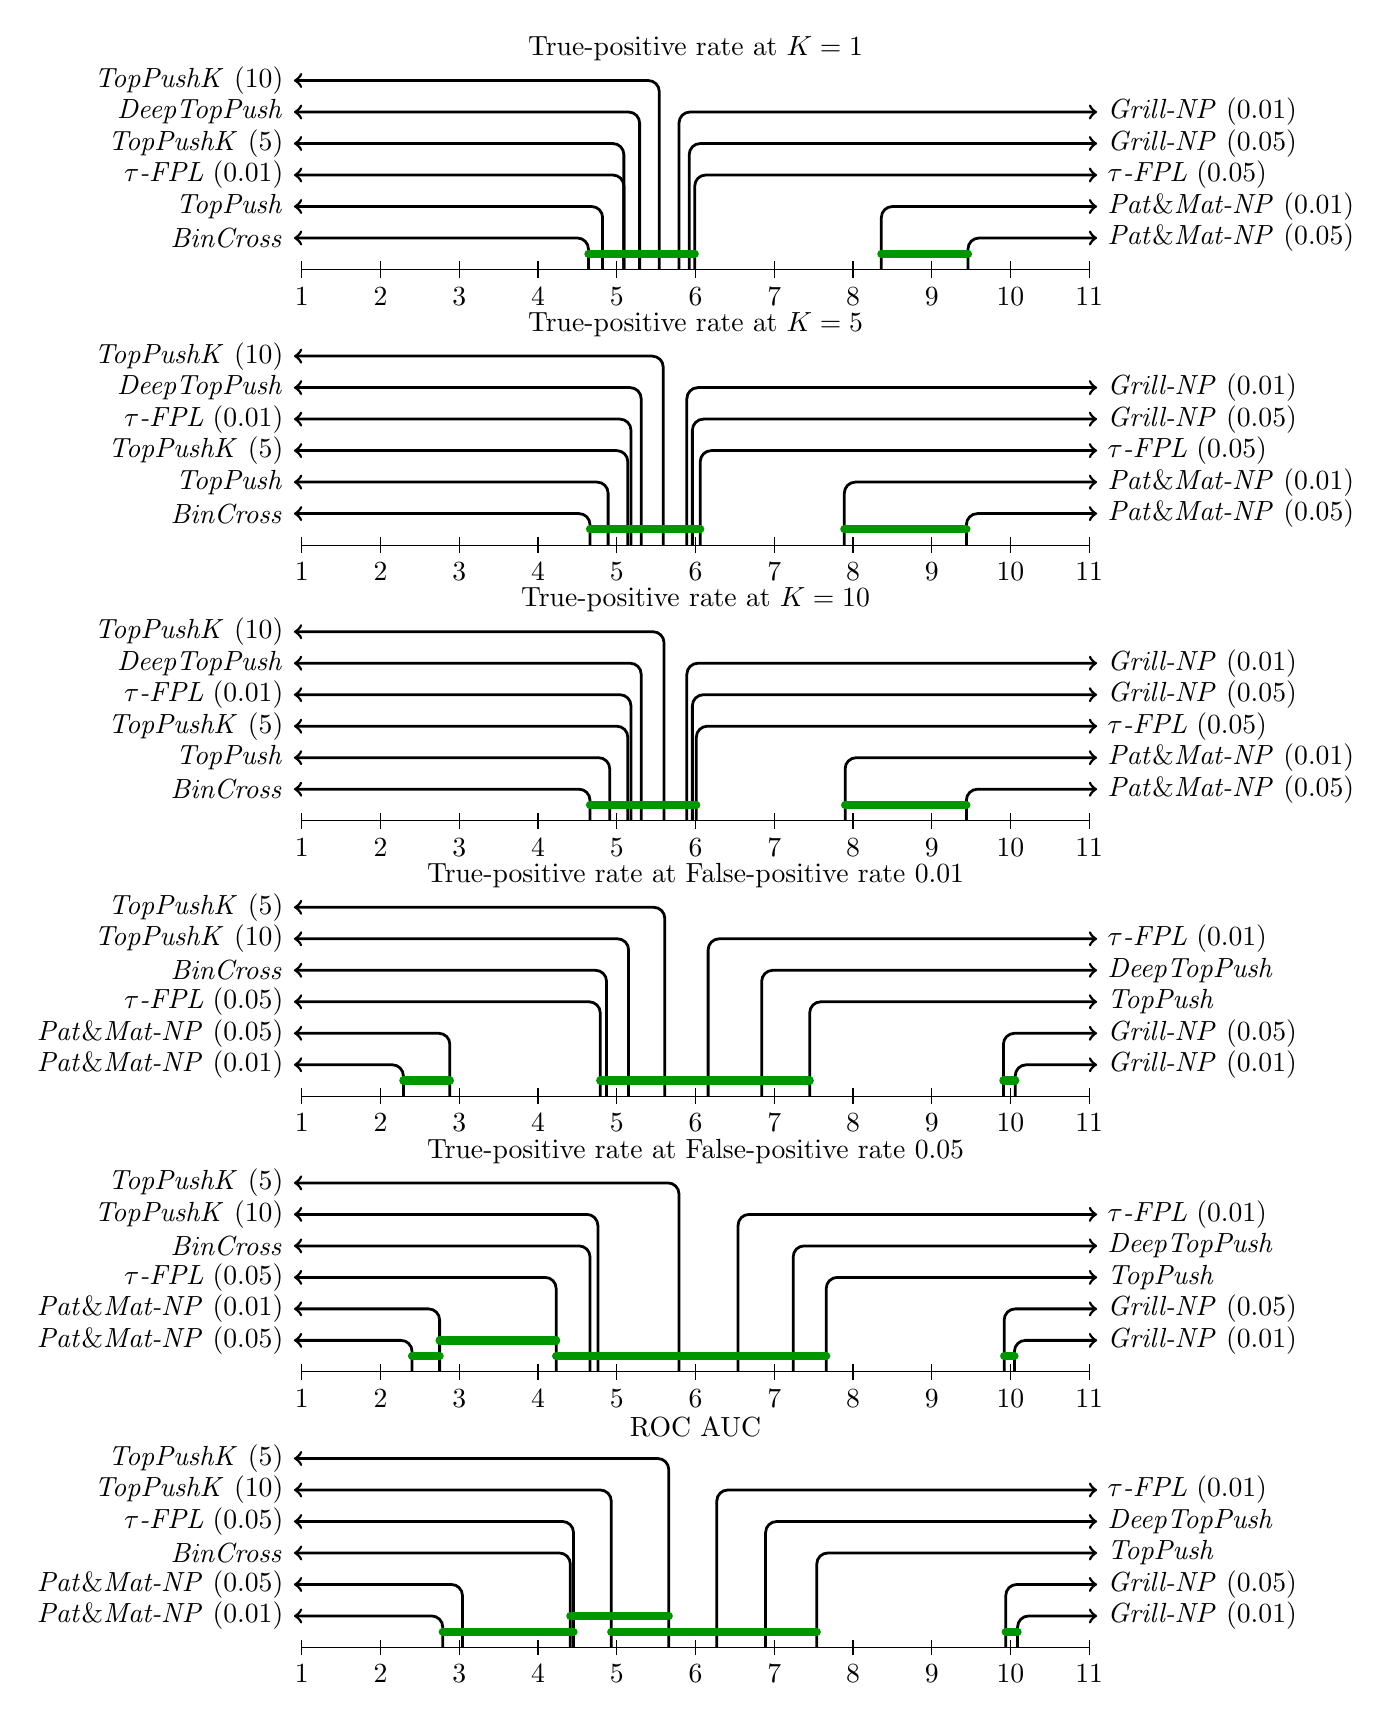
\begin{tikzpicture}
  \node at (6.0,2.8) {ROC AUC}; 
  \draw (1,0) -- (11,0); 
  \foreach \x in {1,...,11} \draw (\x,0.1) -- (\x,-0.1) node[anchor=north]{$\x$}; 
  \draw[line_node] (2.79,0) -- (2.79,0.4) -- (0.9, 0.4) node[anchor=east] {\PatMatNP(0.01)}; 
  \draw[line_node] (3.04,0) -- (3.04,0.8) -- (0.9, 0.8) node[anchor=east] {\PatMatNP(0.05)}; 
  \draw[line_node] (4.41,0) -- (4.41,1.2) -- (0.9, 1.2) node[anchor=east] {\BaseLine}; 
  \draw[line_node] (4.45,0) -- (4.45,1.6) -- (0.9, 1.6) node[anchor=east] {\tauFPL(0.05)}; 
  \draw[line_node] (4.93,0) -- (4.93,2.0) -- (0.9, 2.0) node[anchor=east] {\TopPushK(10)}; 
  \draw[line_node] (5.66,0) -- (5.66,2.4) -- (0.9, 2.4) node[anchor=east] {\TopPushK(5)}; 
  \draw[line_node] (6.27,0) -- (6.27,2.0) -- (11.1, 2.0) node[anchor=west] {\tauFPL(0.01)}; 
  \draw[line_node] (6.89,0) -- (6.89,1.6) -- (11.1, 1.6) node[anchor=west] {\DeepTopPush}; 
  \draw[line_node] (7.54,0) -- (7.54,1.2) -- (11.1, 1.2) node[anchor=west] {\TopPush}; 
  \draw[line_node] (9.94,0) -- (9.94,0.8) -- (11.1, 0.8) node[anchor=west] {\GrillNP(0.05)}; 
  \draw[line_node] (10.09,0) -- (10.09,0.4) -- (11.1, 0.4) node[anchor=west] {\GrillNP(0.01)}; 
  \draw[line_cv] (2.79,0.2) -- (4.45, 0.2); 
  \draw[line_cv] (4.41,0.4) -- (5.66, 0.4); 
  \draw[line_cv] (4.93,0.2) -- (6.27, 0.2); 
  \draw[line_cv] (5.66,0.2) -- (6.89, 0.2); 
  \draw[line_cv] (6.27,0.2) -- (7.54, 0.2); 
  \draw[line_cv] (9.94,0.2) -- (10.09, 0.2); 

  \node at (6.0,6.3) {True-positive rate at False-positive rate $0.05$}; 
  \draw (1,3.5) -- (11,3.5); 
  \foreach \x in {1,...,11} \draw (\x,3.6) -- (\x,3.4) node[anchor=north]{$\x$}; 
  \draw[line_node] (2.4,3.5) -- (2.4,3.9) -- (0.9, 3.9) node[anchor=east] {\PatMatNP(0.05)}; 
  \draw[line_node] (2.75,3.5) -- (2.75,4.3) -- (0.9, 4.3) node[anchor=east] {\PatMatNP(0.01)}; 
  \draw[line_node] (4.23,3.5) -- (4.23,4.7) -- (0.9, 4.7) node[anchor=east] {\tauFPL(0.05)}; 
  \draw[line_node] (4.66,3.5) -- (4.66,5.1) -- (0.9, 5.1) node[anchor=east] {\BaseLine}; 
  \draw[line_node] (4.76,3.5) -- (4.76,5.5) -- (0.9, 5.5) node[anchor=east] {\TopPushK(10)}; 
  \draw[line_node] (5.79,3.5) -- (5.79,5.9) -- (0.9, 5.9) node[anchor=east] {\TopPushK(5)}; 
  \draw[line_node] (6.54,3.5) -- (6.54,5.5) -- (11.1, 5.5) node[anchor=west] {\tauFPL(0.01)}; 
  \draw[line_node] (7.24,3.5) -- (7.24,5.1) -- (11.1, 5.1) node[anchor=west] {\DeepTopPush}; 
  \draw[line_node] (7.66,3.5) -- (7.66,4.7) -- (11.1, 4.7) node[anchor=west] {\TopPush}; 
  \draw[line_node] (9.92,3.5) -- (9.92,4.3) -- (11.1, 4.3) node[anchor=west] {\GrillNP(0.05)}; 
  \draw[line_node] (10.05,3.5) -- (10.05,3.9) -- (11.1, 3.9) node[anchor=west] {\GrillNP(0.01)}; 
  \draw[line_cv] (2.4,3.7) -- (2.75, 3.7); 
  \draw[line_cv] (2.75,3.9) -- (4.23, 3.9); 
  \draw[line_cv] (4.23,3.7) -- (5.79, 3.7); 
  \draw[line_cv] (4.76,3.7) -- (6.54, 3.7); 
  \draw[line_cv] (5.79,3.7) -- (7.24, 3.7); 
  \draw[line_cv] (6.54,3.7) -- (7.66, 3.7); 
  \draw[line_cv] (9.92,3.7) -- (10.05, 3.7); 

  \node at (6.0,9.8) {True-positive rate at False-positive rate $0.01$}; 
  \draw (1,7.0) -- (11,7.0); 
  \foreach \x in {1,...,11} \draw (\x,7.1) -- (\x,6.9) node[anchor=north]{$\x$}; 
  \draw[line_node] (2.29,7.0) -- (2.29,7.4) -- (0.9, 7.4) node[anchor=east] {\PatMatNP(0.01)}; 
  \draw[line_node] (2.88,7.0) -- (2.88,7.8) -- (0.9, 7.8) node[anchor=east] {\PatMatNP(0.05)}; 
  \draw[line_node] (4.79,7.0) -- (4.79,8.2) -- (0.9, 8.2) node[anchor=east] {\tauFPL(0.05)}; 
  \draw[line_node] (4.87,7.0) -- (4.87,8.6) -- (0.9, 8.6) node[anchor=east] {\BaseLine}; 
  \draw[line_node] (5.15,7.0) -- (5.15,9.0) -- (0.9, 9.0) node[anchor=east] {\TopPushK(10)}; 
  \draw[line_node] (5.61,7.0) -- (5.61,9.4) -- (0.9, 9.4) node[anchor=east] {\TopPushK(5)}; 
  \draw[line_node] (6.16,7.0) -- (6.16,9.0) -- (11.1, 9.0) node[anchor=west] {\tauFPL(0.01)}; 
  \draw[line_node] (6.84,7.0) -- (6.84,8.6) -- (11.1, 8.6) node[anchor=west] {\DeepTopPush}; 
  \draw[line_node] (7.45,7.0) -- (7.45,8.2) -- (11.1, 8.2) node[anchor=west] {\TopPush}; 
  \draw[line_node] (9.91,7.0) -- (9.91,7.8) -- (11.1, 7.8) node[anchor=west] {\GrillNP(0.05)}; 
  \draw[line_node] (10.06,7.0) -- (10.06,7.4) -- (11.1, 7.4) node[anchor=west] {\GrillNP(0.01)}; 
  \draw[line_cv] (2.29,7.2) -- (2.88, 7.2); 
  \draw[line_cv] (4.79,7.2) -- (6.16, 7.2); 
  \draw[line_cv] (5.15,7.2) -- (6.84, 7.2); 
  \draw[line_cv] (6.16,7.2) -- (7.45, 7.2); 
  \draw[line_cv] (9.91,7.2) -- (10.06, 7.2); 

  \node at (6.0,13.3) {True-positive rate at $K = 10$}; 
  \draw (1,10.5) -- (11,10.5); 
  \foreach \x in {1,...,11} \draw (\x,10.6) -- (\x,10.4) node[anchor=north]{$\x$}; 
  \draw[line_node] (4.66,10.5) -- (4.66,10.9) -- (0.9, 10.9) node[anchor=east] {\BaseLine}; 
  \draw[line_node] (4.91,10.5) -- (4.91,11.3) -- (0.9, 11.3) node[anchor=east] {\TopPush}; 
  \draw[line_node] (5.14,10.5) -- (5.14,11.7) -- (0.9, 11.7) node[anchor=east] {\TopPushK(5)}; 
  \draw[line_node] (5.18,10.5) -- (5.18,12.1) -- (0.9, 12.1) node[anchor=east] {\tauFPL(0.01)}; 
  \draw[line_node] (5.31,10.5) -- (5.31,12.5) -- (0.9, 12.5) node[anchor=east] {\DeepTopPush}; 
  \draw[line_node] (5.6,10.5) -- (5.6,12.9) -- (0.9, 12.9) node[anchor=east] {\TopPushK(10)}; 
  \draw[line_node] (5.89,10.5) -- (5.89,12.5) -- (11.1, 12.5) node[anchor=west] {\GrillNP(0.01)}; 
  \draw[line_node] (5.96,10.5) -- (5.96,12.1) -- (11.1, 12.1) node[anchor=west] {\GrillNP(0.05)}; 
  \draw[line_node] (6.01,10.5) -- (6.01,11.7) -- (11.1, 11.7) node[anchor=west] {\tauFPL(0.05)}; 
  \draw[line_node] (7.9,10.5) -- (7.9,11.3) -- (11.1, 11.3) node[anchor=west] {\PatMatNP(0.01)}; 
  \draw[line_node] (9.44,10.5) -- (9.44,10.9) -- (11.1, 10.9) node[anchor=west] {\PatMatNP(0.05)}; 
  \draw[line_cv] (4.66,10.7) -- (6.01, 10.7); 
  \draw[line_cv] (7.9,10.7) -- (9.44, 10.7); 

  \node at (6.0,16.8) {True-positive rate at $K = 5$}; 
  \draw (1,14.0) -- (11,14.0); 
  \foreach \x in {1,...,11} \draw (\x,14.1) -- (\x,13.9) node[anchor=north]{$\x$}; 
  \draw[line_node] (4.66,14.0) -- (4.66,14.4) -- (0.9, 14.4) node[anchor=east] {\BaseLine}; 
  \draw[line_node] (4.89,14.0) -- (4.89,14.8) -- (0.9, 14.8) node[anchor=east] {\TopPush}; 
  \draw[line_node] (5.14,14.0) -- (5.14,15.2) -- (0.9, 15.2) node[anchor=east] {\TopPushK(5)}; 
  \draw[line_node] (5.18,14.0) -- (5.18,15.6) -- (0.9, 15.6) node[anchor=east] {\tauFPL(0.01)}; 
  \draw[line_node] (5.31,14.0) -- (5.31,16.0) -- (0.9, 16.0) node[anchor=east] {\DeepTopPush}; 
  \draw[line_node] (5.59,14.0) -- (5.59,16.4) -- (0.9, 16.4) node[anchor=east] {\TopPushK(10)}; 
  \draw[line_node] (5.89,14.0) -- (5.89,16.0) -- (11.1, 16.0) node[anchor=west] {\GrillNP(0.01)}; 
  \draw[line_node] (5.96,14.0) -- (5.96,15.6) -- (11.1, 15.6) node[anchor=west] {\GrillNP(0.05)}; 
  \draw[line_node] (6.06,14.0) -- (6.06,15.2) -- (11.1, 15.2) node[anchor=west] {\tauFPL(0.05)}; 
  \draw[line_node] (7.89,14.0) -- (7.89,14.8) -- (11.1, 14.8) node[anchor=west] {\PatMatNP(0.01)}; 
  \draw[line_node] (9.44,14.0) -- (9.44,14.4) -- (11.1, 14.4) node[anchor=west] {\PatMatNP(0.05)}; 
  \draw[line_cv] (4.66,14.2) -- (6.06, 14.2); 
  \draw[line_cv] (7.89,14.2) -- (9.44, 14.2); 

  \node at (6.0,20.3) {True-positive rate at $K = 1$}; 
  \draw (1,17.5) -- (11,17.5); 
  \foreach \x in {1,...,11} \draw (\x,17.61) -- (\x,17.39) node[anchor=north]{$\x$}; 
  \draw[line_node] (4.64,17.5) -- (4.64,17.9) -- (0.9, 17.9) node[anchor=east] {\BaseLine}; 
  \draw[line_node] (4.82,17.5) -- (4.82,18.3) -- (0.9, 18.3) node[anchor=east] {\TopPush}; 
  \draw[line_node] (5.09,17.5) -- (5.09,18.7) -- (0.9, 18.7) node[anchor=east] {\tauFPL(0.01)}; 
  \draw[line_node] (5.09,17.5) -- (5.09,19.1) -- (0.9, 19.1) node[anchor=east] {\TopPushK(5)}; 
  \draw[line_node] (5.29,17.5) -- (5.29,19.5) -- (0.9, 19.5) node[anchor=east] {\DeepTopPush}; 
  \draw[line_node] (5.54,17.5) -- (5.54,19.9) -- (0.9, 19.9) node[anchor=east] {\TopPushK(10)}; 
  \draw[line_node] (5.79,17.5) -- (5.79,19.5) -- (11.1, 19.5) node[anchor=west] {\GrillNP(0.01)}; 
  \draw[line_node] (5.92,17.5) -- (5.92,19.1) -- (11.1, 19.1) node[anchor=west] {\GrillNP(0.05)}; 
  \draw[line_node] (5.99,17.5) -- (5.99,18.7) -- (11.1, 18.7) node[anchor=west] {\tauFPL(0.05)}; 
  \draw[line_node] (8.36,17.5) -- (8.36,18.3) -- (11.1, 18.3) node[anchor=west] {\PatMatNP(0.01)}; 
  \draw[line_node] (9.46,17.5) -- (9.46,17.9) -- (11.1, 17.9) node[anchor=west] {\PatMatNP(0.05)}; 
  \draw[line_cv] (4.64,17.7) -- (5.99, 17.7); 
  \draw[line_cv] (8.36,17.7) -- (9.46, 17.7); 
\end{tikzpicture}
\end{document}

  \caption{\textbf{Primal formulations with non-linear model:} Critical difference (CD) diagrams (level of importance 0.05) of the Nemenyi post hoc test for the Friedman test. Each diagram shows the mean rank of each method, with rank 1 being the best. Green wide horizontal lines group together methods with the mean ranks that are not significantly different. The critical difference diagrams were computed for mean rank averages over all datasets.}
  \label{fig: critical diagrams primal NN}
\end{figure}

\newpage

\section{Steganalysis}

In the previous section, we presented results on standard image recognition datasets. Even though the results are quite good even on these datasets, they did not fully show the importance of the problem of classification at the top. To show the importance of this problem properly,  we need to find the field in which the maximizing true-positive rate at the low false-positive rate is an important task. Such a field can be for example steganography and steganalysis. The standard way how to share secret information these days is the use of encryption. However, in such a case, the presence of a secret message (even though encrypted) is obvious. Steganography aims to hide the fact that communication taking place, by hiding the secret message within an ordinary file (usually called cover file) in order to avoid detection. The secret message is then extracted at its destination. The secret data can be hidden in almost any type of digital content, however the most popular are images. There are two reasons for this. The first of them is the ubiquity of images on the Internet and therefore the ease to use them as cover files for secret messages. The second reason is their large potential payload, i.e. it is possible to hide a lot of information in the images with high resolution. With an appropriate cover image and steganography tools, it is possible to create an stego-image (image with a hidden message) that can not be recognized from the cover image by human perception. However, each tool leaves a fingerprint or signature in the image, that can be used to detect stego images. The field that tries to detect stego images and possibly decrypt messages from them is called steganalysis. In steganalysis, the goal is to achieve the best true-positive rate with the lowest possible false-positive rate. Therefore steganalysis is the branch suitable for the classification at the top, since many of the formulations derived in this work focus precisely on this task. \cite{morkel2005overview, silman2001steganography} 

For the eperiments, we have a large dataset of cover-images that consists of approximately 450 000 images from Flickr. All these images are in the JPEG format with quality factor 80. Since the dataset does not contain any stego images, we use two different ways to generate them. For the purpose of this work, we named them \textbf{Nsf5} and \textbf{JMiPOD}.

\subsection{Nsf5}

In this case, we generate stego images using simulated F5 with matrix embedding turned off and we use payload 0.2. Since we are interested in low false-positive rates, we need a lot of negative (cover) samples to estimate it. This is evident in~\eqref{eq: patmat np} where the threshold~$t$ is a surrogate approximation of false-positive rate, i.e., the threshold is computed only from negative samples. Positive (stego) samples occurs only in the objective function. Since generating of stego images is expensive and we do not need them to estimate false-positive rate, we decided to use 10\% of all cover images to generate their stego counterparts. All images (both cover and stego images) are then described using 22 500 features and split into train / validation / test set in ratio 0.45 / 0.05 / 0.5. The resulting sizes of train / validation / test splits as well as the number of stego images in them, are in Table~\ref{tab: datasets summary}. 

Since the resulting classification task is relatively easier to solve, we decided to use a simple linear model. The number o training samples and their size is not too big, therefore we can load the whole dataset into memory. It allows us to use full gradient descent instead of its stochastic version. As an optimizer, we use the ADAM~\cite{kingma2014adam} with default settings and fixed step length~$\alpha = 0.01.$ We also use a fixed number of epochs to 1000 for all formulations. Finally, we repeat each experiment ten times with ten different random seeds.

Figure~\ref{fig: steganalysis nsf5} shows ROC curves for the test set of \textbf{Nsf5} dataset. For simplicity, we show ROC curves only for one run of the experiment. Moreover, Table~\ref{tab: steganalysis nsf5} shows seven different performance metrics computed for each formulation. Each shown result in this table is a median of ten independent runs. It is evident, that \BaseLine provides very poor results for all metrics except the $\auroc$. Surprisingly, \BaseLine is the worst even for the $\auroc.$ On the other hand, \DeepTopPush excels at very low false-positive rates, as can be seen from both the table and the figure. In fact, \DeepTopPush provides the best results for four out of seven performance metrics (the best results are highlighted in green). Note that all these four metrics operate at extremely small false-positive rates. We can also see, that \PatMatNP($10^{-5}$) is the best at false-positive rate~$10^{-4}$. This unexpected result is probably caused by the approximation of the true top $\tau$-quantile of all scores of negative samples in \PatMatNP formulation. Therefore, \PatMatNP($10^{-5}$) is optimized for a false-positive rate slightly higher than~$10^{-5}$ and as a consequence outperforms \PatMatNP($10^{-5}$) at false-positive rate~$10^{-4}$. Similar behavior can be seen for \PatMatNP($10^{-4}$) and \PatMatNP($10^{-3}$) at false-positive rate~$10^{-4}$.

\begin{figure}
  \centering
  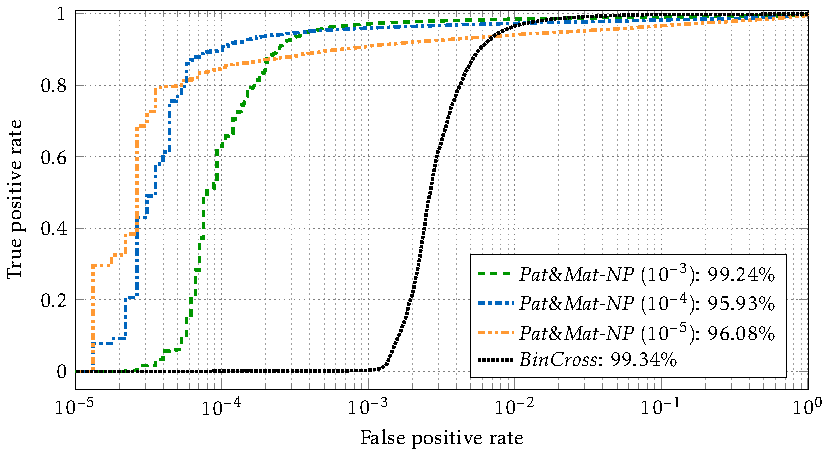
\includegraphics{images/stego_nsft5.pdf}
  \caption{\textbf{Nsf5 dataset:} ROC curves with logaithmic $x$-axis.}
  \label{fig: steganalysis nsf5}
\end{figure}

\begin{table}[!t]
  \centering
  \begin{NiceTabular}{lccccccc}
    \CodeBefore
    \rowcolor{\headercol}{1-2}
    \rowcolors{4}{\rowcol}{}[restart]
    \Body
    \toprule
    \Block[c]{2-1}{\textbf{Formulation}}
    & \Block[c]{2-1}{$\auroc$}
    & \Block[c]{1-3}{$\tpratk$}
    &&& \Block[c]{1-3}{$\tpratfpr$} \\
    \cline{3-8}
    && $1$
    & $10$
    & $5$
    & $10^{-5}$
    & $10^{-4}$
    & $10^{-3}$ \\
    \midrule
    \BaseLine
    & \worst{95.84}
    & \worst{0.0}
    & \worst{0.0}
    & \worst{0.0}
    & \worst{0.0}
    & \worst{0.02}
    & \worst{0.7} \\
    \DeepTopPush
    & 98.29
    & \best{5.07}
    & \best{35.48}
    & \best{57.66}
    & \best{48.65}
    & 89.56
    & 93.67 \\
    \PatMatNP($10^{-5}$)
    & 98.81
    & 2.55
    & 23.02
    & 47.24
    & 35.28
    & \best{91.9}
    & 95.84 \\
    \PatMatNP($10^{-4}$)
    & 98.98
    & \worst{0.0}
    & 0.05
    & 4.34
    & 1.78
    & 79.76
    & \best{96.18} \\
    \PatMatNP($10^{-3}$)
    & \best{99.26}
    & \worst{0.0}
    & \worst{0.0}
    & 0.01
    & \worst{0.0}
    & 0.29
    & 91.98 \\
    \bottomrule
  \end{NiceTabular}
  \caption{\textbf{NSF5 dataset:}  All presented results are medians of ten independent runs with different random seeds. Each column of the table corresponds to one performance metric and every row to one formulation. The best result for each metric is highlighted in green, while the worst result is highlighted in red.}
  \label{tab: steganalysis nsf5}
\end{table}

\subsection{JMiPOD}

In this case, we first select all images that can be cropped to to size $256 \times 256 \times 3$ and than cropped them looselesly using \emph{jpegtran} library. Than, we use JMiPOD~\cite{cogranne2020steganography} algorithm to generate stego images with payload 0.1. We use the same approach as in the case of Nsf5 dataset and use only 10\% of cover images to generate their stego counterparts. We split the data into train / validation / test set in ratio 0.375 / 0.125 / 0.5. The resulting sizes of train / validation / test splits as well as the number of stego images in them, are in Table~\ref{tab: datasets summary}. 

In this case, the resulting classification task is quite complicated, therefore we decided to use pre-trained EfficientNet-B0~\cite{tan2019efficientnet} as a model. Originally the model is trained for 1000 classes, therefore, we removed the last fully-connected layer and replaced it with a randomly initialized fully-connected layer of appropriate size for binary classification. The resulting model is large and therefore it is not possible to use a full gradient. For this reason, we use stochastic gradient descent with balanced mini-batches of size 256. As an optimizer, we use the ADAM~\cite{kingma2014adam} with default settings and fixed step length~$\alpha = 0.01.$ Finally, we use a fixed number of epochs to 30 for all formulations and we repeat each experiment ten times with ten different random seeds.

\begin{figure}[!t]
  \centering
  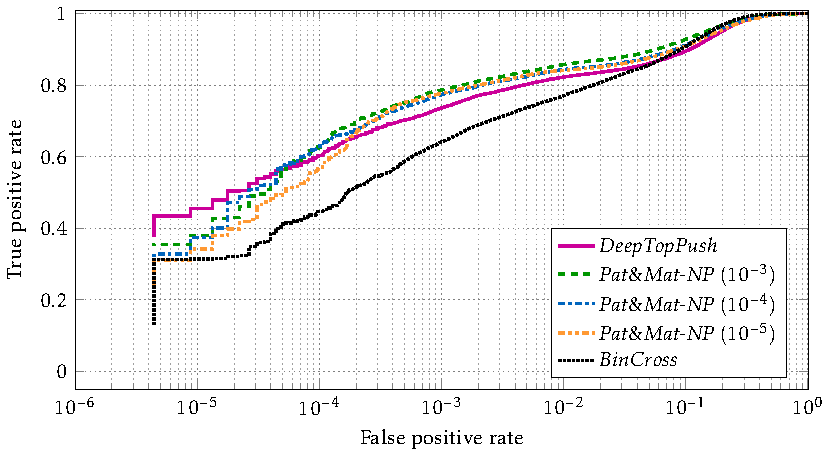
\includegraphics{images/stego_jmipod.pdf}
  \caption{\textbf{JMiPOD dataset:} ROC curves with logaithmic $x$-axis.}
  \label{fig: steganalysis jmipod}
\end{figure}

\begin{table}[!t]
  \centering
  \begin{NiceTabular}{lccccccc}
    \CodeBefore
      \rowcolor{\headercol}{1-2}
      \rowcolors{4}{\rowcol}{}[restart]
    \Body
    \toprule
    \Block[c]{2-1}{\textbf{Formulation}}
      & \Block[c]{2-1}{$\auroc$}
      & \Block[c]{1-3}{$\tpratk$}
      &&& \Block[c]{1-3}{$\tpratfpr$} \\
    \cline{3-8}
      && $1$
      & $10$
      & $5$
      & $10^{-5}$
      & $10^{-4}$
      & $10^{-3}$ \\
    \midrule
    \BaseLine
      & 97.5
      & \worst{13.52}
      & \worst{24.65}
      & \worst{29.54}
      & \worst{27.28}
      & \worst{44.58}
      & \worst{63.84} \\
    \DeepTopPush
      & \worst{97.26}
      & \best{34.25}
      & \best{42.57}
      & \best{47.3}
      & \best{43.59}
      & 60.42
      & 73.67 \\
    \PatMatNP($10^{-5}$)
      & 97.66
      & 21.24
      & 31.6
      & 39.38
      & 33.54
      & 60.35
      & 78.04 \\
    \PatMatNP($10^{-4}$)
      & 97.49
      & 25.66
      & 36.76
      & 45.19
      & 38.28
      & 63.49
      & 77.43 \\
    \PatMatNP($10^{-3}$)
      & \best{98.0}
      & 26.99
      & 38.76
      & 44.83
      & 42.17
      & \best{64.5}
      & \best{78.11} \\
    \bottomrule
  \end{NiceTabular}
  \caption{\textbf{JMiPOD dataset:} All presented results are medians of ten independent runs with different random seeds. Each column of the table corresponds to one performance metric and every row to one formulation. The best result for each metric is highlighted in green, while the worst result is highlighted in red.}
  \label{tab: steganalysis jmipod}
\end{table}

As in the previous subsection, Figure~\ref{fig: steganalysis jmipod} shows ROC curves for the test set of \textbf{JMiPOD} dataset, and Table~\ref{tab: steganalysis jmipod} shows seven performance metrics. Each shown result in this table is a median of ten independent runs. Since trained models use stochastic gradient descent, the results are not as evident as in the case of Nsf5 dataset. \BaseLine still provides the worst results for most of the metrics, but the differences are much smaller than for the Nsf5 dataset. We can see, that \DeepTopPush again provides the best performance for 4 of 7 metrics. It shows that the enhanced minibatch used in \DeepTopPush Algorithm~\ref{alg: deep toppush} improves the approximation quality of the true threshold and therefore it reduces the bias of sampled gradient (as we already showed in Figure~\ref{fig:thresholds2}). Even though \PatMatNP($10^{-3}$), \PatMatNP($10^{-4}$) and \PatMatNP($10^{-5}$) were trained for different levels of false-positive rate, they all perform similarly. As we said before, the decision threshold~$t$ of \PatMatNP model is the approximation of true top $\tau$-quantile of all scores of negative samples. Since we use minibatches with 128 negative samples, the smallest quantile that can be found on this minibatch is~$\tau = \frac{1}{128}=0.0078125.$ If we try to approximate smaller quantiles, we always get the same results. Therefore, \PatMatNP($10^{-3}$), \PatMatNP($10^{-4}$), \PatMatNP($10^{-5}$) should work almost identically, and we can see from both the figure and the table, that these three formulations provide very similar results.

\section{Malware Detection}

In the previous section, we presented results from the domain of steganalysis. Another domain in which formulations from presented framework can be very useful, is the domain of malware detection. As an example, consider standard antivirus software on a personal computer. Every user wants to be protected, so the goal of antivirus software is to detect as much malware as possible. However, if the antivirus software is too restrictive, it can easily happen, that clean software is marked as malware, i.e. the antivirus software can easily produce false alarms. If the antivirus software produces false alarms too often, it can be very annoying to the user and may lead to uninstalling the antivirus software. Therefore, the goal of every antivirus software is to maximize a true-positive rate at a very low false-positive rate, which is precisely what the formulations from the framework do.

In this section, we presented results on a real-world dataset provided by a renowned cybersecurity company. The dataset consists of malware analysis reports of executable files. This is an extremely tough dataset as individual samples are JSON files whose size ranges from 1kB to 2.5MB. The structure of the sample is highly complicated because each sample has a different number of features, and features may have a complicated structure, such as a list of ports to which the file connects. This is in sharp contrast with standard datasets, where each sample has the same number of features, and each feature is a real number. The usual approach how to process such complicated data is to create manually feature vectors and use them for training instead of the original data. However, such an approach is extremely time-demanding and requires expert knowledge of the original data. For this reason, we decided to use a different approach that is called Hierarchical Multiple Instance Learning (HMIL)~\cite{pevny2017using}. For the training, we use a publicly available implementation of HMIL~\cite{mandlik2021mill}, which allows train models directly from JSON files without the necessity of complicated feature extraction.

Since the dataset is very large (see Table~\ref{tab: datasets summary}), we train each formulation only one time. Moreover, we use only the formulations that worked the best in the previous experiments, i.e. we use only the \BaseLine, \PatMatNP($10^{-2}$), \PatMatNP($10^{-3}$) and \BaseLine. As an optimizer, we use the ADAM~\cite{kingma2014adam} with default settings and fixed step length~$\alpha = 0.01.$ We also use balanced mini-batches of size 2000, which allows us to obtain a very good estimate of the true thresholds as discussed in Section~\ref{sec: biased threshold estimate}. Finally, we use a fixed number of epochs to 100 for all formulations.

Figure~\ref{fig: malware detection} shows the performance of all formulations on the test set. For the comparison, we use ROC curves and we use filled circles to highlight the thresholds for which the formulation were optimized. It is clear, that \DeepTopPush is the best at low false-positive rates. Even at the extremely low false positive rate $\tau=10^{-5}$, \DeepTopPush correctly identified $46\%$ of malware. We can also see, that \PatMatNP($10^{-3}$) is the best at false-positive rate~$10^{-3}$, which is exactly the point for which the formulation should be optimized. However, \DeepTopPush performs almost as well as \PatMatNP($10^{-3}$) at this false-positive rate. Finally, at the false-positive rate~$10^{-2}$ all formulations perform equally well.

\begin{figure}
  \centering
  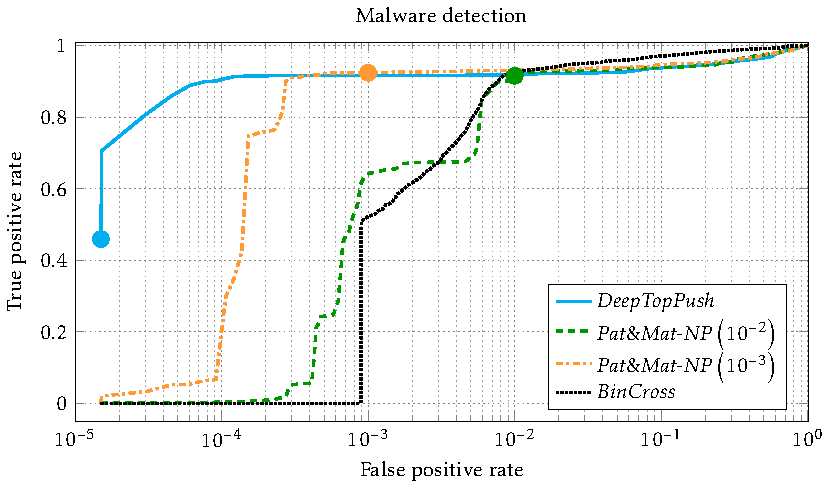
\includegraphics{images/malware_detection.pdf}
  \caption{\textbf{Malware detection:} ROC curves with logaithmic $x$-axis. The circles show the thresholds the formulations were optimized for.}
  \label{fig: malware detection}
\end{figure}

\chapter{Conclusion}

\section{Linear Model}

In this paper, we achieved the following results:
\begin{itemize}
  \item We presented a unified framework for the three criteria from Chapter~\ref{chap: framework}. These criteria include ranking, accuracy at the top and hypothesis testing.
  \item We showed that several known methods (\TopPush, \Grill, \tauFPL) fall into our framework and derived some completely new methods (\PatMat, \PatMatNP).
  \item We performed a theoretical analysis of the methods. We showed that known methods suffer from certain disadvantages. While \TopPush and \tauFPL are sensitive to outliers, \Grill is non-convex. We proved the global convergence of the stochastic gradient descent for \PatMat and \PatMatNP.
  \item We performed a numerical comparison and we showed a good performance of our method \PatMatNP.
\end{itemize}


\section{Dual}\label{sec:Conclusion}

In this paper, we analyzed and extended the general framework for binary classification on top samples from~\cite{adam2021general} to nonlinear problems. Achieved results can be summarized as follows:
\begin{itemize}
    \item We derived the dual formulations for \TopPush, \TopPushK and \PatMat.
    \item We proposed a new method for solving the dual problems. We performed its complexity analysis. For selected surrogate functions we also derived the exact formulas needed in the method.
    \item We performed a numerical analysis of the proposed method. We showed its good convergence as well as improved performance of nonlinear kernels over the linear one.
\end{itemize}
Based on the numerical analysis from Section~\ref{sec:Numerical experiments}, we recommend using \TopPush or \TopPushK for problems where the resulting recall should be small. Otherwise, we recommend using \PatMat with an appropriately selected~$\tau$ parameter.

\section{Neural Networks}

We proposed \DeepTopPush as an efficient method for solving the constrained non-decomposable problem of accuracy at the top, which focuses on the performance only above a threshold. We implicitly removed some optimization variables, created an unconstrained end-to-end network and used the stochastic gradient descent to train it. We modified the minibatch so that the sampled threshold (computed on a minibatch) is a good estimate of the true threshold (computed on all samples). We showed both theoretically and numerically that this procedure reduces the bias of the sampled gradient. The time increase over the standard method with no threshold is small. We demonstrated the usefulness of \DeepTopPush both on visual recognition datasets, a ranking problem and on a real-world application of malware detection.


% ------------------------------------------------------------------------------
% Appendix
% ------------------------------------------------------------------------------
\part*{Apendices}
\appendix

\chapter{Appendix for Chapter~\ref{chap: framework}}

Here, we provide additional results and proofs of results mentioned in the main body. For convenience, we repeat the result statements. To show this equivalence of \eqref{eq: aatp original} and \eqref{eq: aatp original combination}, we will start with an auxiliary lemma.

\lemmaequivalence*
\begin{proof}[Proof Lemma~\ref{lemma:fnfp_equivalence} on page~\pageref{lemma:fnfp_equivalence}]
  By the definition of the quantile we have
  \begin{equation*}
    \tp(\bm{s},t)+\fp(\bm{s},t) = n\tau + q-1.
  \end{equation*}
  This implies
  \begin{equation*}
    \fp(\bm{s},t)=n\tau +q - 1-\tp(\bm{s},t) =n\tau+q-1-\npos +\fn(\bm{s},t).
  \end{equation*}
  From this relation we deduce
  \begin{equation*}
    \begin{aligned}
      \fp(\bm{s},t)
      & = \mu \fp(\bm{s},t) + (1 - \mu)\fp(\bm{s},t) \\
      & = \mu \fp(\bm{s},t) + (1 - \mu)\Brac{\fn(\bm{s},t) + n\tau - \npos + q - 1} \\
      & = \mu \fp(\bm{s},t) + (1 - \mu)\fn(\bm{s},t) + (1-\mu)\Brac{n\tau - \npos} + (1-\mu)\Brac{q - 1},
    \end{aligned}
  \end{equation*}
  which is precisely the lemma statement.
\end{proof}

\chapter{Appendix for Chapter~\ref{chap: linear}}
\section{Convexity}

\propconvex*
\begin{proof}[Proof of Proposition~\ref{prop: convexity} on page~\pageref{prop: convexity}]
  From Notation~\ref{not: scores}, threshold~$t_0$ is just a maximum from vector~$\bm{s}^-$ of scores of all negative samples.  Since maximum is a convex function, threshold T is a convex function of weights~$\bm{w}.$ Moreover, it is easy to show that the quantile~$t_1$ is not convex. Due to~\cite{lapin2015top}, the mean of the~$K$ highest values of a vector is a convex function. Therefore, threshold~$t_2$ is a convex function  of weights~$\bm{w}.$ It remains to analyze threshold~$t_3.$ Let us define function~$g$ as follows
  \begin{equation*}
    g(\bm{w},t) := \frac{1}{n} \sum_{i \in \I} l(\bm{w}^{\top} \bm{x}_i - t) - \tau.
  \end{equation*}
  where we for simplicity set~$\vartheta = 1.$ Then~$t_3$ is defined via an implicit equation~$g(\bm{w},t) = 0.$ Moreover, since~$l$ is convex, we immediately obtain that~$g$ is jointly convex in both variables. To show the convexity, consider~$\bm{w}, \; \tilde{\bm{w}} \in \R^d$ and the corresponding thresholds~$t = t_3(\bm{w})$,~$\tilde{t} = t_3(\tilde{\bm{w}})$. Then for any~$\lambda\in[0,1],$ we have 
  \begin{equation}\label{eq:proof_conv1}
    g\Brac{\lambda \bm{w} + (1 - \lambda)\tilde{\bm{w}}, \;\lambda t + (1 - \lambda)\tilde{t}}
    \leq \lambda g(\bm{w}, t) + (1 - \lambda) g(\tilde{\bm{w}}, \tilde{t}) = 0.
  \end{equation}
  The inequality follows from the convexity of~$g$  and the equality from~$g(\bm{w}, t) = g(\tilde{\bm{w}}, \tilde{t}) = 0,$ which holds due to the definition of~$t_3.$ From the definition of~$t_3,$ we also have
  \begin{equation}\label{eq:proof_conv2}
    g(\lambda\bm{w} + (1-\lambda)\tilde{\bm{w}}, \; t_3(\lambda\bm{w} + (1-\lambda)\tilde{\bm{w}})) = 0.
  \end{equation}
  Since~$g$ is non-increasing in the second variable, from~\eqref{eq:proof_conv1} and~\eqref{eq:proof_conv2} we deduce
  \begin{equation*}
    t_3(\lambda\bm{w} + (1-\lambda)\tilde{\bm{w}})
    \leq \lambda t + (1-\lambda)\tilde{t}
    =   \lambda t_3(\bm{w})+(1-\lambda) t_3(\tilde{\bm{w}}),
  \end{equation*}
  which implies that function~$\bm{w}\mapsto t_3(\bm{w})$ is convex.
\end{proof}

\thmconvex*
\begin{proof}[Proof of Theorem~\ref{thm: convexity} on page~\pageref{thm: convexity}]
  Due to the definition~\eqref{eq: confusion counts surrogate}, the objective function~$L$ equals to
  \begin{equation*}
    L(\bm{w}) = \fns(\bm{s}, t(\bm{w})) = \sum_{i \in \Ipos} l \Brac{t(\bm{w}) - \bm{w}^{\top} \bm{x}_i}.
  \end{equation*}
  Here we write~$t(\bm{w})$ to stress the dependence of~$t$ on~$\bm{w}$. Since~$\bm{w}\mapsto t(\bm{w})$ is a convex function, we also have that~$\bm{w} \mapsto t(\bm{w}) - \bm{w}^{\top} \bm{x}$ is a convex function. From its definition, the surrogate function~$l$ is convex and non-decreasing.  Since the composition of a convex function with a non-decreasing convex function is a convex function, this finishes the proof.
\end{proof}

\section{Differentiability}

\derivative* 
\begin{proof}[Proof of Theorem~\ref{thm: differentiability} on page~\pageref{thm: differentiability}]
  The non-differentiability of~$t_0,$~$t_1$ and~$t_2$ happens whenever the threshold value is achieved at two different scores. The result for~$t_3$ follows directly from the implicit function theorem. 
\end{proof}

\newpage

\section{Stability}\label{app: stability}

\degeneratebehavior*

Additionally to the assumptions from Example~\ref{ex: degenerate behaviour}, we consider the hinge loss function and no regularization for all formulations from Table~\ref{tab: summary formulations}. We also assume that~$n$ is large, and the outlier may be ignored for the computation of thresholds that require a large number of points. Since the computation is simple for other formulations, we show it only for \PatMat. For~$\bm{w}_0 = (0,0),$ we have
\begin{equation*}
  \tau
  = \frac{1}{n}\sum_{i \in \I} l\Brac{\vartheta(\bm{w}_0^\top \bm{x}_i - t)}
  = l(0 - \vartheta t) = 1 - \vartheta t,
\end{equation*}
which implies that threshold~$t$ equals~$t = \nicefrac{1-\tau}{\vartheta}.$ Consequently, the value of the objective function is
\begin{equation}\label{eq: PatMat objective 0}
  L(\bm{w}_0)
    = \frac{1}{\npos} \sum_{i \in \Ipos} l(t - \bm{w}_0^\top \bm{x}_i)
    = l(t - 0)
    = 1 + t,
\end{equation}
where the last equality follows from the definition of the hinge loss function and the fact that~$t \geq 0.$ This finishes the computation for~$\bm{w}_0$. For~$\bm{w}_1 = (1,0),$ the computation goes similar. Since all samples are uniformly distributed in~$[-1,1]\times[-1,1],$ scores~$\bm{w}_1^\top \bm{x}_i$ for~$i \in \I$ are uniformly distributed in~$[-1,1].$ Then, if the scaling parameter~$\vartheta$ satisfies~$\vartheta \leq \tau$, we have
\begin{align*}
  \tau
    & = \frac{1}{n} \sum_{i \in \I} l\Brac{\vartheta (\bm{w}_1^\top \bm{x}_i - t)}
    \approx \frac{1}{2}\int_{-1}^{1} l\Brac{\vartheta(s-t)} \dd{s}
      = \frac{1}{2} \int_{-1}^{1} \max\{0, 1 + \vartheta(s - t)\}\dd{s} \\
    & =\frac{1}{2} \int_{-1}^{1} (1+\vartheta(s - t))\dd{s}
      = 1 - \vartheta t + \frac{\vartheta}{2}\int_{-1}^{1}s\dd{s}
      = 1 - \vartheta t.
\end{align*}
which again implies that threshold~$t$ equals~$t = \nicefrac{1-\tau}{\vartheta}$. Note that we could ignore the~$\max$ operator in the relation above, since 
\begin{equation*}
  1 + \vartheta(s - t)
    \geq 1 + \vartheta(-1 - t)
    = 1 + \vartheta(-1 - \frac{1 - \tau}{\vartheta})
    = \tau - \vartheta
    \geq 0.
\end{equation*}
Finally, since positive samples are uniformly distributed in~$[0,1]\times[-1,1],$ corresponding scores $\bm{w}_1^\top \bm{x}_i$  for~$i \in \Ipos$ are uniformly distributed in~$[0,1].$ Therefore, for the objective function, we have
\begin{equation*}
  L(\bm{w}_1)
    = \frac{1}{\npos} \sum_{i \in \Ipos} l(t - \bm{w}_1^\top \bm{x}_i)
    \approx \int_{0}^{1} l(t-s)\dd{s}
    = \int_{0}^{1} (1 + t - s)\dd{s}
    = 0.5 + t.
\end{equation*}
Results for \PatMatNP can be obtained in a similar way.

\pagebreak

\larget*
\begin{proof}[Proof of Theorem~\ref{thm:large_t} on page~\pageref{thm:large_t}]
  All mentioned formulations use surogate approximation of the false-negative rate as the objective function~$L.$ For the linear classifier, the objective function has the following form
  \begin{equation*}
    L(\bm{w})
      = \frac{1}{\npos}\sum_{i \in \Ipos}l(t - \bm{w}^{\top} \bm{x}_i)
  \end{equation*}
  Due to~$l(0) = 1$ and the convexity of~$l$ we have~$l(s) \geq 1 + cs$, where~$c$ equals to the derivative of~$l$ at~$0$. Then we have
  \begin{equation*}
    L(\bm{w}) 
      \geq \frac{1}{\npos} \sum_{i \in \Ipos}(1 + c(t-\bm{w}^{\top} \bm{x}_i))
      = 1 + c\Brac{t - \frac{1}{\npos}\sum_{i \in \Ipos}\bm{w}^{\top} \bm{x}}
      \geq 1,
  \end{equation*}
  where the last inequality follows from assumption~\eqref{eq:w_zero_nn}. Now we realize that for any formulation from the statement, the corresponding threshold for~$\bm{w}=0$ equals to~$t=0$, and thus~$L(\bm{0})=1$. But then~$L(\bm{0}) \leq L(\bm{w})$. The second part of the result follows from the form of thresholds~$t(\bm{w})$.
\end{proof}

\patmatzero*
\begin{proof}[Proof of Theorem~\ref{thm:patmat_zero} on page~\pageref{thm:patmat_zero}]
  Firstly recall thewe use linear model and Notation~\ref{not: scores} and define the following auxilliary variables
  \begin{equation*}
    \begin{aligned}
      s_{\min} & = \min \Set{s_i}{i \in \I}, \qquad
      s_{\max} & = \max \Set{s_i}{i \in \I}, \qquad
      \bar{s} & = \frac{1}{n} \sum_{i \in \I} s_i. \\
    \end{aligned}
  \end{equation*}
  Using the definition of~$\bar{s}$ we get the following relation
  \begin{equation}\label{eq:patmat_zero_aux0}
    \bar{s}
      = \frac{1}{n} \sum_{i \in \I} s_i
      = \frac{1}{n}\sum_{i \in \Ipos} s_i + \frac{1}{n} \sum_{i \in \Ineg} s_i
      < \frac{1}{n} \sum_{i \in \Ipos} s_i + \frac{\nneg}{n\npos} \sum_{i \in \Ipos} s_i
      = \frac{1}{\npos} \sum_{i \in \Ipos} s_i,
  \end{equation}
  where the inequality follows from~\eqref{eq:patmat_zero} and the last equality follows from
  \begin{equation*}
    \frac{1}{n} + \frac{\nneg}{n\npos}
      = \frac{1}{n} \Brac{1 + \frac{\nneg}{\npos}} 
      = \frac{1}{n} \frac{\npos + \nneg}{\npos}
      = \frac{1}{n} \frac{n}{\npos}
      = \frac{1}{\npos}.
  \end{equation*}
  Moreover, since the average of elements of the  vector is smaller or equal to the maximum of elements of the same vector, we get the following relation
  \begin{equation*}
    \bar{s}
      < \frac{1}{\npos} \sum_{i \in \Ipos} s_i
      \leq \max \Set{s_i}{i \in \Ipos}
      \leq \max \Set{s_i}{i \in \I}
      = s_{\max}
  \end{equation*}
  where the first inequality follows from~\eqref{eq:patmat_zero_aux0}. The lower bound for~$\bar{s}$ can be computed in a similar way. Altogether, we have~$s_{\min} < \bar{s} < s_{\max}$. Then we can define
  \begin{equation*}
    \vartheta_0 = \min\Brac[c]{\frac{\tau}{\bar{s} - s_{\min}}, \; \frac{1-\tau}{s_{\max}-\bar{s}}, \; \tau},
  \end{equation*}
  observe that~$\vartheta_0 > 0$, fix any~$\vartheta \in (0, \vartheta_0)$ and define
  \begin{equation*}
    t = \frac{1 - \tau}{\vartheta} + \bar{s}.
  \end{equation*}
  Then we obtain for any~$i \in \I$
  \begin{equation*}
    1 + \vartheta(s_i - t)
      \geq 1 + \vartheta(s_{\min} - t)
      = 1 + \vartheta s_{\min} - 1 + \tau - \vartheta\bar{s}
      = \tau - \vartheta (\bar{s} - s_{\min}),
  \end{equation*}
  where the first equality follows from the definition of~$t.$ From the definition~$\vartheta_0$ we known the following
  \begin{equation*}
    0 < \vartheta \leq \vartheta_0 \leq \frac{\tau}{\bar{s} - s_{\min}}.
  \end{equation*}
  Since~$\bar{s} - s_{\min} > 0,$ we get the following inequality
  \begin{equation}\label{eq:patmat_zero_aux1}
    1 + \vartheta(s_i - t)
      = \tau - \vartheta (\bar{s} - s_{\min})
      \geq \tau - \frac{\tau}{\bar{s} - s_{\min}} (\bar{s} - s_{\min})
      = 0
  \end{equation}
  Moreover, combining the definition of the hinge loss function in Notation~\ref{not: surrogates} and the inequality above, we have
  \begin{equation*}
    l\Brac{\vartheta (s_i - t)} = \max\{0, 1 + \vartheta (s_i - t), 0\} = \Brac{1 + \vartheta(s_i - t)}.
  \end{equation*}
  Finally, replacing the hinge loss in the left hand side of~\eqref{eq: aatp quantile surrogate} leads to
  \begin{equation*}
    \begin{aligned}
      \frac{1}{n} \sum_{i \in \I} l\Brac{\vartheta (s_i - t)}
      & = \frac{1}{n}\sum_{i \in \I}\Brac{1 + \vartheta(s_i - t)} \\
      & = 1 - \vartheta t + \frac{\vartheta}{n} \sum_{i \in \I} s_i \\
      & = 1 - \vartheta \Brac{\frac{1 - \tau}{\vartheta} + \bar{s}} + \vartheta \bar{s} \\
      & = \tau,
    \end{aligned}
  \end{equation*}
  where the third equality employs the definition of~$\bar{s}$ and~$t$. But this means that~$t$ is the threshold corresponding to~$\bm{w}$, i.e. it solves~\eqref{eq: aatp quantile surrogate}. Similarly to~\eqref{eq:patmat_zero_aux1} we get
  \begin{equation}\label{eq:patmat_zero_aux2}
    1 + t - s_i
    \geq 1 + t-s_{\max}
    =   1 + \frac{1-\tau}{\vartheta} + \bar{s} - s_{\max}
    \geq \frac{1-\tau}{\vartheta} + \bar{s} - s_{\max}
    \geq 0,
  \end{equation}
  where the last inequality follows from the definition of~$\vartheta_0$. Then for the objective we have
  \begin{equation*}
    \begin{aligned}
      L(\bm{w}) = \frac{1}{\npos}\sum_{i \in \Ipos}l(t-s_i)
      & = \frac{1}{\npos}\sum_{i \in \Ipos}\Brac{1+t-s_i} \\
      & = 1 + t - \frac{1}{\npos}\sum_{i \in \Ipos} s_i \\
      & < 1 + \Brac{\frac{1 - \tau}{\vartheta} + \bar{s}} - \bar{s} \\
      & = 1 + \frac{1-\tau}{\vartheta} \\
      & = L(\bm{0}),\\
    \end{aligned}
  \end{equation*}
  where the second equality follows from~\eqref{eq:patmat_zero_aux2}, the only inequality from~\eqref{eq:patmat_zero_aux0} and the last equality from~\eqref{eq: PatMat threshold 0} and~\eqref{eq: PatMat objective 0}. Thus, we finished the proof for \PatMat. The proof for \PatMatNP can be performed in an identical way by replacing in the definition of~$\bar{s}$ the mean with respect to all samples by the mean with respect to all negative samples.
\end{proof}

\section{Threshold comparison}\label{app:relations}

Whenever the objective contains only false-negatives, a lower threshold~$t$ means a lower objective function. Therefore, a lower threshold is preferred. The two following lemmas compares thresholds defined in Chapter~\ref{chap: framework} in terms of approximation quality.
\begin{lemma}[Thresholds relation~\cite{zhang2018tau}]\label{prop: threholds}
  We always have
  \begin{equation*}
    t_1(\bm{s}) \leq t_2(\bm{s}) \leq t_3(\bm{s}).
  \end{equation*}
\end{lemma}



\begin{lemma}\label{lemma:thresholds2}
  Consider the \Grill, \GrillNP, \TopMeanK and \tauFPL formulations and the notation from Notation~\ref{not: scores}. Then we have the following statements:
  \begin{equation*}
    \begin{aligned}
      s_{[\npos\tau]}^+ > s_{[\nneg\tau]}^-
        & \implies \Grill \text{ has larger threshold than }\GrillNP, \\
      \frac{1}{\npos\tau}\sum_{i=1}^{\npos\tau} s_{[i]}^+
      > \frac{1}{\nneg\tau}\sum_{i=1}^{\nneg\tau} s_{[i]}^-
        & \implies \TopMeanK \text{ has larger threshold than }\tauFPL. \\
    \end{aligned}
  \end{equation*}
\end{lemma}

\begin{proof}
  Since~$\bm{s}^+$ and~$\bm{s}^-$ are computed on disjunctive indices, we have
  \begin{equation*}
    s_{[n\tau]} \geq \min\{s_{[\npos\tau]}^+, \; s_{[\nneg\tau]}^-\}.
  \end{equation*}
  Since~$s_{[n\tau]}$ is the threshold for \Grill and~$s_{[\nneg\tau]}^-$ is the threshold for \GrillNP, the first statement follows. The second part can be shown in a similar way.
\end{proof}
  
\noindent Since the goal of the presented formulations is to push~$s^+$ above~$s^-$, we may expect that the conditions in Lemma~\ref{lemma:thresholds2} hold true. 

\section{Computing the threshold for \PatMat}\label{app:threshold}

We show how to efficiently compute the threshold~\eqref{eq: aatp quantile surrogate} for \PatMat with linear model and the hinge surrogate from Notation~\ref{not: surrogates}. Consider function
\begin{equation}\label{eq:defin_h}
  h(t) = \sum_{i \in \I} l\Brac{\vartheta(s_i - t)} - n\tau.
\end{equation}
Then solving~\eqref{eq:update_t} is equivalent to looking for~$\hat{t}$ such that~$h(\hat{t}) = 0$. Function~$h$ is continuous and strictly decreasing (until it hits the global minimum) with~$h(t) \to \infty$ as~$t \to -\infty$ and~$h(t) \to -n\tau$ as~$t \to \infty$. Thus, there is a unique solution to the equation~$h(t) = 0$. For sorted data, the following lemma gives advice on how to solve equation~$h(t) = 0$. 

\begin{lemma}
  Consider vector of scores~$\bm{s}$ and its sorted version~$\bm{s}_{[\cdot]}$ with decreasing elements as defined in Notation~\ref{not: scores}. Define~$\gamma = \nicefrac{1}{\vartheta}$. Then 
  \begin{equation}\label{eq:update_h}
    h(s_{[j]} + \gamma) = h(s_{[j - 1]} + \gamma) + (j - 1) \vartheta(s_{[j - 1]} - s_{[j]})
  \end{equation}
  for all~$i = 2, \; 3, \ldots, n$ with the initial condition~$h(s_{[1]} + \gamma) = -n\tau$.
\end{lemma}
\begin{proof}
Observe first that
\begin{equation*}
  \begin{aligned}
    h(s_{[j]}+\gamma)
      & = \sum_{i \in \I} l\Brac{\vartheta(s_i - (s_{[j]} + \gamma))} - n\tau \\
      & = \sum_{i \in \I} \max\Brac[c]{0,\; 1 + \vartheta\Brac{s_i - s_{[j]} - \frac{1}{\gamma}}} - n\tau \\
      & = \sum_{i = 1}^{j - 1} \vartheta(s_{[i]} - s_{[j]}) - n\tau,
  \end{aligned}
\end{equation*}
where the last equality holds since~$\vartheta > 0$ and~$s_{[i]} - s_{[j]} \leq 0$ for all~$i \geq j$
From here, we obtain~$h(s_{[1]} + \gamma) = -n\tau$. Moreover, we have
\begin{equation*}
  \begin{aligned}
    h(s_{[j]} + \gamma)
    & = \sum_{i = 1}^{j - 1} \vartheta(s_{[i]} - s_{[j]}) - n\tau \\
    & = \sum_{i = 1}^{j - 2} \vartheta(s_{[i]} - s_{[j]}) + \vartheta(s_{[j-1]} - s_{[j]}) - n\tau \\
    & = \sum_{i = 1}^{j - 2} \vartheta(s_{[i]} - s_{[j]} \pm s_{[j - 1]}) + \vartheta(s_{[j-1]} - s_{[j]}) - n\tau \\
    & = \sum_{i = 1}^{j - 2} \vartheta(s_{[i]} - s_{[j - 1]}) + \sum_{i = 1}^{j - 2} \vartheta(s_{[j - 1]} - s_{[j]}) + \vartheta(s_{[j - 1]} - s_{[j]}) - n\tau \\
    & = h(s_{[j - 1]} + \gamma) + (j - 1) \vartheta(s_{[j - 1]} - s_{[j]}),
  \end{aligned}
\end{equation*}
which finishes the proof.
\end{proof}

\noindent Thus, to solve~$h(t) = 0$ with the hinge surrogate, we start with~$t_1 = s_{[1]}  + \gamma$ and~$h(t_1) = -n\tau$. Then we start decreasing~$t$ according to~\eqref{eq:update_h} until we find some~$t_i = s_{[i]} + \gamma$ such that~$h(t_i) > 0$. The desired~$t$ then lies between~$t_i$ and~$t_{i-1}$. Since~$h$ is a piecewise linear function with
\begin{equation*}
  h(t) = h(t_{i-1}) + \frac{t - t_{i-1}}{t_{i} - t_{i-1}}\Brac{h(t_{i}) - h(t_{i-1})}
\end{equation*}
for~$t \in [t_{i-1}, \; t_{i}]$, the precise value of~$\hat{t}$ can be computed by a simple interpolation
\begin{equation*}
  \hat{t}
    = t_{i-1} - h(t_{i-1})\frac{t_{i} - t_{i-1}}{h(t_{i}) - h(t_{i-1})}
    = t_{i-1} - h(t_{i-1})\frac{t_{i} - t_{i-1}}{-(i-1)\vartheta(t_{i} - t_{i-1})}
    = t_{i-1} + \frac{h(t_{i-1})}{\vartheta(i-1)}.
\end{equation*}

\section{Convergence of stochastic gradient descent}

The proof is divided into three parts. In Section~\ref{app:sgd1}, we prove a general statement for convergence of stochastic gradient descent with a convex objective. In Section~\ref{app:sgd2} we apply it to Theorem~\ref{thm:sgd}. The proof is based on auxiliary results from Section~\ref{app:sgd3}.

\subsection{General result}\label{app:sgd1}

Consider a differentiable objective function~$L$ and the optimization method
\begin{equation}\label{eq:update}
  \bm{w}^{k+1} = \bm{w}^k - \alpha^k g(\bm{w}^k),
\end{equation}
where~$\alpha^k > 0$ is a stepsize and~$g(\bm{w}^k)$ is an approximation of the gradient~$\nabla L(\bm{w}^k)$. Assume the following:
\begin{enumerate}[label={(A\arabic*)}]
  \item \label{ass_convex}~$L$ is differentiable, convex and attains a global minimum;
  \item \label{ass_gbound}~$\norm{g(\bm{w}^k)}\leq B$ for all~$k$;
  \item \label{ass_alpha1} the stepsize is non-increasing and satisfies~$\sum_{k=0}^\infty \alpha^k = \infty$;
  \item \label{ass_alpha2} the stepsize satisfies~$\sum_{k=0}^\infty (\alpha^k)^2<\infty$;
  \item \label{ass_alpha3} the stepsize satisfies~$\sum_{k=0}^\infty \norm{\alpha^{k+1}-  \alpha^k}<\infty$.
\end{enumerate}
Assumptions~\ref{ass_alpha1}-\ref{ass_alpha3} are satisfied for example for~$\alpha^k = \nicefrac{\alpha^0}{k+1}$. We start with the general result.

\begin{theorem}\label{thm:convergence}
  Assume that~\ref{ass_convex}-\ref{ass_alpha2} is satisfied. If there exists some~$C$ such that for some global minimum of~$\bm{w}^*$ of~$L$ we have
  \begin{equation}\label{eq:nec_cond}
    \sum_{k=0}^\infty \alpha^k \inner{g(\bm{w}^k) - \nabla L(\bm{w}^k)}{\bm{w}^* - \bm{w}^k} \leq C,
  \end{equation}
  then the sequence~$\{\bm{w}^k\}$ generated by~\eqref{eq:update} is bounded and~$L(\bm{w}^k) \to L(\bm{w}^*)$. Thus, all its convergent subsequences converge to some global minimum of~$L$.
\end{theorem}
\begin{proof}
  Note first that the convexity of~$L$ from~\ref{ass_convex} implies
  \begin{equation}\label{eq:convex_estimate}
    \inner{\nabla L(\bm{w}^k)}{\bm{w}^* - \bm{w}^k} \leq L(\bm{w}^*) - L(\bm{w}^k).
  \end{equation}
  Then we have
  \begin{equation*}
    \begin{aligned}
      \norm{\bm{w}^{k+1} - \bm{w}^*}^2
        = \; & \norm{\bm{w}^k - \alpha^k g(\bm{w}^k) - \bm{w}^*}^2 \\
        = \; &\norm{\bm{w}^k - \bm{w}^*}^2 + 2\alpha^k\inner{g(\bm{w}^k)}{\bm{w}^* - \bm{w}^k} + (\alpha^k)^2 \norm{g(\bm{w}^k)}^2 \\
        \leq \; &\norm{\bm{w}^k - \bm{w}^*}^2 + 2\alpha^k\inner{g(\bm{w}^k) \pm \nabla L(\bm{w}^k)}{\bm{w}^* - \bm{w}^k} + (\alpha^k)^2 B^2\\
        \leq \; & \norm{\bm{w}^k - \bm{w}^*}^2 + 2 \alpha^k \inner{g(\bm{w}^k) - \nabla L(\bm{w}^k)}{\bm{w}^* - \bm{w}^k} \\
        & + 2 \alpha^k \Brac{L(\bm{w}^*) - L(\bm{w}^k)} + (\alpha^k)^2 B^2,
    \end{aligned}
  \end{equation*}
  where the first inequality follows from assumption~\ref{ass_gbound} and the second on from the properties of inner product and~\eqref{eq:convex_estimate}. Summing this expression for all~$k$ and using~\eqref{eq:nec_cond} leads to
  \begin{equation*}
    \limsup_{k \rightarrow \infty} \; \norm{\bm{w}^k - \bm{w}^*}^2
      \leq \norm{\bm{w}^0 - \bm{w}^*}^2 + 2C + 2 \sum_{k=0}^\infty \alpha^k (L(\bm{w}^*) - L(\bm{w}^k)) + \sum_{k=0}^ \infty (\alpha^k)^2 B^2.
\end{equation*}
  Using assumption~\ref{ass_alpha2} results in the existence of some~$\hat{C}$ such that
  \begin{equation}\label{eq:general_bound}
  \limsup_{k \rightarrow \infty} \;\norm{\bm{w}^k - \bm{w}^*}^2 + 2\sum_{k=0}^\infty \alpha^k \Brac{L(\bm{w}^k) - L(\bm{w}^*)} \leq 2 \hat{C}.
  \end{equation}
  Since~$\alpha^k > 0$ and~$L(\bm{w}^k) \geq L(\bm{w}^*)$ as~$\bm{w}^*$ is a global minimum of~$L$, we infer that sequence~$\{\bm{w}^k\}$ is bounded and~\eqref{eq:general_bound} implies
  \begin{equation*}
    \sum_{k=0}^\infty \alpha^k \Brac{L(\bm{w}^k) - L(\bm{w}^*)} \leq \hat{C}.
  \end{equation*}
  Since~$L(\bm{w}^k) - L(\bm{w}^*) \geq 0$, due to assumption~\ref{ass_alpha1} we obtain
  \begin{equation*}
    \lim_{k \to \infty} L(\bm{w}^k) = L(\bm{w}^*),
  \end{equation*}
  which implies the theorem statement.
\end{proof}

\subsection{Proof of Theorem~\ref{thm:sgd}}\label{app:sgd2}

For the proof, we will consider a general surrogate which satisfies:
\begin{enumerate}[label={(S\arabic*)}]
  \item \label{surr_basic1} $l(s)\geq 0$ for all~$s\in\R$, $l(0)=1$ and~$l(s)\to 0$ as~$s\to-\infty$;
  \item \label{surr_basic2} $l$ is convex and strictly increasing function on~$(s_0,\infty)$, where~$s_0:=\sup\{s \mid l(s)=0\}$;
  \item \label{surr_ratio} $\nicefrac{l'}{l}$ is a decreasing function on~$(s_0,\infty)$;
  \item \label{surr_der1} $l'$ is a bounded function;
  \item \label{surr_der2} $l'$ is a Lipschitz continuous function with Lipschitz constant~$D$.
\end{enumerate}
All these reguirements are satisfied for the surrogate logistic or by the Huber loss, which is the hinge surrogate which is smoothened on an~$\varepsilon$-neighborhood of zero.

\sgd*
\begin{proof}[Proof of Theorem~\ref{thm:sgd} on page~\pageref{thm:sgd}]
  We intend to apply Theorem~\ref{thm:convergence} and thus, we need to verify its assumptions. Assumption~\ref{ass_convex} is satisfied as~$L$ is convex due to Theorem~\ref{thm: convexity}. Assumption~\ref{ass_gbound} follows directly from Lemma~\ref{lemma:bound_g}. Assumptions~\ref{ass_alpha1},\ref{ass_alpha2} and~\ref{ass_alpha3} are imposed directly in the statement of this theorem. It remains to verify~\eqref{eq:nec_cond}.

  For simplicity, we will do so only for~$\vartheta = 1$ and for~$2$ minibatches of the same size. However, the proof would be identical for other values. This implies that there are some~$\Imb^k$ and~$\Imb^{k+1}$ which are pairwise disjoint, they cover all samples and that~$\Imb^k = \Imb^{k+2}$ for all~$k$. The assumptions imply that the number of positive samples in each minibatch equal to~$\nmbpos^k = \nicefrac{\npos}{2}$, where~$\npos$ is the total number of positive samples.

  First we estimate the difference between~$s_i^k$ defined in~\eqref{eq:defin_z} and~$\bm{x}_i^\top \bm{w}^k$. For any~$i \in \Imb^k$ we have
  \begin{equation*}
    s_i^k = \bm{x}_i^\top \bm{w}^k
  \end{equation*}
  and since we have two disjoint minibatches, due to the construction~\eqref{eq:defin_z} we get
  \begin{equation}\label{eq:sgd_estimate_z1}
    \begin{aligned}
      s_i^{k-1}
          = s_i^{k-2}
        & = \bm{x}_i^\top \bm{w}^{k-2} \\
        & = \bm{x}_i^\top \Brac{\bm{w}^k + \alpha^{k-2}g(\bm{w}^{k-2}) + \alpha^{k-1} g(\bm{w}^{k-1})} \\
        & = \bm{x}_i^\top \bm{w}^k + \alpha^{k-2}\bm{x}_i^\top g(\bm{w}^{k-2}) + \alpha^{k-1}\bm{x}_i^\top g(\bm{w}^{k-1}).
    \end{aligned}
  \end{equation}
  Similarly, due to the construction~\eqref{eq:defin_z}, for~$i \notin \Imb^k$ we have
  \begin{equation}\label{eq:sgd_estimate_z2}
    s_i^k
    = s_i^{k-1}
    = \bm{x}_i^\top \bm{w}^{k-1}
    = \bm{x}_i^\top (\bm{w}^k+\alpha^{k-1}g(\bm{w}^{k-1}))
    = \bm{x}_i^\top \bm{w}^k + \alpha^{k-1}\bm{x}_i^\top g(\bm{w}^{k-1}).
  \end{equation}
  Recall that we already verified~\ref{ass_convex}-\ref{ass_alpha3}. Combining~\ref{ass_gbound} with~\eqref{eq:sgd_estimate_z1} and~\eqref{eq:sgd_estimate_z2} yields the existence of some~$C_2$ such that for all~$i \in \I$ we have
  \begin{equation}\label{eq:estimate_diff_z}
    \begin{aligned}
      \norm{s_i^k - \bm{x}_i^\top \bm{w}^k} &\leq C_2\alpha^{k-1}, \\
      \norm{s_i^{k-1} - \bm{x}_i^\top \bm{w}^k} &\leq C_2\Brac{\alpha^{k-1}+\alpha^{k-2}}. \\
    \end{aligned}
  \end{equation}
  This also immediately implies
  \begin{equation}\label{eq:estimate_diff_t}
    \begin{aligned}
      \norm{t^k - t(\bm{w}^k)}     & \leq C_2\alpha^{k-1}, \\
      \norm{t^{k-1} - t(\bm{w}^k)} & \leq C_2\Brac{\alpha^{k-1}+\alpha^{k-2}}. \\
    \end{aligned}
  \end{equation}
  Since~$l'$ is Lipschitz continuous with Lipschitz constant~$D$ according to~\ref{surr_der2}, due to~\eqref{eq:estimate_diff_z} and~\eqref{eq:estimate_diff_t} we get
  \begin{equation}\label{eq:sgd_lipschitz1}
    \begin{aligned}
      \norm{l'(t^k-s_i^k) - l'(t(\bm{w}^k)-\bm{x}_i^\top \bm{w}^k)}
        & \leq D \norm{t^k-s_i^k - t(\bm{w}^k)+ \bm{x}_i^\top \bm{w}^k}
        \leq  2C_2 D \alpha^{k-1}.
    \end{aligned}
  \end{equation}
  In an identical way we can show
  \begin{equation}\label{eq:sgd_lipschitz2}
    \begin{aligned}
      \norm{l'(t^{k-1}-s_i^{k-1}) - l'(t(\bm{w}^k)-\bm{x}_i^\top \bm{w}^k)}
        & \leq 2C_2D\Brac{\alpha^{k-1}+\alpha^{k-2}}, \\
      \norm{l'(s_i^k-t^k) - l'(\bm{x}_i^\top \bm{w}^k-t(\bm{w}^k))}
        & \leq 2C_2D\alpha^{k-1}, \\
      \norm{l'(s_i^{k-1}-t^{k-1}) - l'(\bm{x}_i^\top \bm{w}^k-t(\bm{w}^k))}
        & \leq 2C_2D\Brac{\alpha^{k-1}+\alpha^{k-2}}.
    \end{aligned}
  \end{equation}
  Now we need to estimate the distance between~$\nabla t(\bm{w}^k)$ and~$\nabla t^k$. From~\eqref{eq:update_nablat} and~\eqref{eq:update_a}, we have
  \begin{equation*}
    \nabla t^k
      = \frac{\sum_{i \in \Imb^k} l'(s_i^k - t^k)\bm{x}_i + \sum_{i \in \Imb^{k-1}} l'(s_i^{k-1} - t^{k-1}) \bm{x}_i}{\sum_{i \in \I} l'(s_i^k - t^k)}.
  \end{equation*}
  Moreover, using Theorem~\ref{thm: differentiability} and the fact that we have only two minibatches and therefore for any~$k$ we have~$\I = \Imb^k \cup \Imb^{k-1}$, we get
  \begin{equation*}
    \nabla t(\bm{w}^k)
      = \frac{\sum_{i \in \Imb^k} l'(\bm{x}_i^\top \bm{w}^k - t(\bm{w}^k))\bm{x}_i + \sum_{i \in \Imb^{k-1}} l'(\bm{x}_i^\top \bm{w}^k - t(\bm{w}^k))\bm{x}_i}{\sum_{i \in \I} l'(\bm{x}_i^\top \bm{w}^k - t(\bm{w}^k))}.
  \end{equation*}
  From Lemma~\ref{lemma:bound_zero} we deduce that the denominators in the relations above are bounded away from zero uniformly in~$k$. Assumption~\ref{ass_alpha2} implies ~$\alpha^k \to 0$. This allows us to use Lemma~\ref{lemma:ratio} which together with~\eqref{eq:sgd_lipschitz2} implies that there is some~$C_3$ such that for all sufficiently large~$k$ we have
  \begin{equation}\label{eq:sgd_nablat_diff}
    \norm{\nabla t^k - \nabla t(\bm{w}^k)} \leq C_3\Brac{\alpha^{k-1} + \alpha^{k-2}}.
  \end{equation}
  Using the assumptions above, we can simplify the terms for~$g(\bm{w}^k)$ and~$\nabla L(\bm{w}^k)$ to
  \begin{equation*}
    \begin{aligned}
      g(\bm{w}^k)
        & = \frac{2}{\npos} \sum_{i \in \Imbpos^k} l'(t^k - s_i^k)(\nabla t^k - \bm{x}_i), \\
      g(\bm{w}^{k+1})
        & = \frac{2}{\npos} \sum_{i \in \Imbpos^{k+1}} l'(t^{k+1}-s_i^{k+1})(\nabla t^{k+1} - \bm{x}_i), \\
      \nabla L(\bm{w}^k)
        & = \frac{1}{\npos} \sum_{i \in \Ipos} l'(t(\bm{w}^k) - \bm{x}_i^\top \bm{w}^k)(\nabla t(\bm{w}^k) - \bm{x}_i), \\
      \nabla L(\bm{w}^{k+1})
        & = \frac{1}{\npos} \sum_{i \in \Ipos} l'(t(\bm{w}^{k+1}) - \bm{x}_i^\top \bm{w}^{k+1})(\nabla t(\bm{w}^{k+1}) - \bm{x}_i).
    \end{aligned}
  \end{equation*}
  Due to the assumptions, we have~$\Ipos = \Imbpos^k \cup \Imbpos^{k+1}$ and~$\emptyset = \Imbpos^k \cap \Imbpos^{k+1}$, which allows us to write
  \begin{subequations}\label{eq:sgd_sum}
    \begin{align}
    \label{eq:sgd_sum1}
    \npos & \Brac{g(\bm{w}^k) + g(\bm{w}^{k+1}) - \nabla f(\bm{w}^k)-\nabla f(\bm{w}^{k+1})}\\
    \label{eq:sgd_sum2}
    & = \sum_{i \in \Imbpos^k} l'(t^k - s_i^k)(\nabla t^k - \bm{x}_i) - \sum_{i \in \Imbpos^k} l'(t(\bm{w}^k) - \bm{x}_i^\top \bm{w}^k)(\nabla t(\bm{w}^k) - \bm{x}_i) \\
    \label{eq:sgd_sum3}
    & + \sum_{i \in \Imbpos^k} l'(t^k - s_i^k)(\nabla t^k - \bm{x}_i) - \sum_{i \in \Imbpos^k} l'(t(\bm{w}^{k+1}) - \bm{x}_i^\top \bm{w}^{k+1})(\nabla t(\bm{w}^{k+1}) - \bm{x}_i)\\
    \label{eq:sgd_sum4}
    & + \sum_{i \in \Imbpos^{k+1}} l'(t^{k+1} - s_i^{k+1})(\nabla t^{k+1} - \bm{x}_i) - \sum_{i\in \Imbpos^{k+1}}l'(t(\bm{w}^k) - \bm{x}_i^\top \bm{w}^k)(\nabla t(\bm{w}^k) - \bm{x}_i) \\
    \label{eq:sgd_sum5}
    & + \sum_{i \in \Imbpos^{k+1}} l'(t^{k+1} - s_i^{k+1})(\nabla t^{k+1} - \bm{x}_i)  - \sum_{i \in \Imbpos^{k+1}} l'(t(\bm{w}^{k+1}) - \bm{x}_i^\top \bm{w}^{k+1})(\nabla t(\bm{w}^{k+1}) - \bm{x}_i).
    \end{align}
  \end{subequations}
  Then relations~\eqref{eq:sgd_nablat_diff} and~\eqref{eq:sgd_lipschitz1} applied to Lemma~\ref{lemma:product} imply
  \begin{multline*}
    \norm{\sum_{i \in \Imbpos^k} l'(t^k - s_i^k)(\nabla t^k - \bm{x}_i) - \sum_{i \in \Imbpos^k} l'(t(\bm{w}^k) - \bm{x}_i^\top \bm{w}^k)(\nabla t(\bm{w}^k) - \bm{x}_i)}\\
      \leq C_4 \Brac{\alpha^{k-1} + \alpha^{k-2}}
  \end{multline*}
  for some~$C_4$, which gives a bound for~\eqref{eq:sgd_sum2}. Bound for~\eqref{eq:sgd_sum5} is obtained by increasing~$k$ by one. Bounds for~\eqref{eq:sgd_sum3} and~\eqref{eq:sgd_sum4} can be find similarly using~\eqref{eq:sgd_lipschitz2}. Altogether, we showed
  \begin{equation}\label{eq:nec_cond3}
    \norm{g(\bm{w}^k) + g(\bm{w}^{k+1}) - \nabla L(\bm{w}^k) - \nabla L(\bm{w}^{k+1})}
      \leq C_1(\alpha^{k-2} + \alpha^{k-1} + \alpha^{k} + \alpha^{k+1})
  \end{equation}
  for some~$C_1$. We now estimate
  \begin{equation}\label{eq:proof_est1}
    \begin{aligned}
      \alpha^k
      & \inner{ g(\bm{w}^{k})-\nabla L(\bm{w}^{k})}{\bm{w}^*-\bm{w}^{k}} + \alpha^{k+1}\inner{ g(\bm{w}^{k+1})-\nabla L(\bm{w}^{k+1})}{\bm{w}^*-\bm{w}^{k+1}} \\
      & = \inner{ g(\bm{w}^{k})-\nabla L(\bm{w}^{k})}{\alpha^k(\bm{w}^*-\bm{w}^{k})}
        + \inner{ g(\bm{w}^{k+1})-\nabla L(\bm{w}^{k+1})}{\alpha^{k+1}(\bm{w}^*-\bm{w}^{k+1})} \\
      & = \inner{ g(\bm{w}^{k})-\nabla L(\bm{w}^{k}) + g(\bm{w}^{k+1})-\nabla L(\bm{w}^{k+1})}{\alpha^k(\bm{w}^*-\bm{w}^{k})} \\
      & + \inner{ g(\bm{w}^{k+1})-\nabla L(\bm{w}^{k+1})}{\alpha^{k+1}(\bm{w}^*-\bm{w}^{k+1})-\alpha^k(\bm{w}^*-\bm{w}^{k})}.
    \end{aligned}
  \end{equation}
  To estimate the second part of the right hand side of~\eqref{eq:proof_est1}, we make use of Lemma~\ref{lemma:bound_g} to obtain the existence of some~$C_5$ such that
  \begin{equation}\label{eq:proof_est2}
    \begin{aligned}
    & \inner{ g(\bm{w}^{k+1})
    -\nabla L(\bm{w}^{k+1})}{\alpha^{k+1}(\bm{w}^*-\bm{w}^{k+1})-\alpha^k(\bm{w}^*-\bm{w}^{k})} \\
    & \leq 2B\norm{\alpha^{k+1}(\bm{w}^*-\bm{w}^{k+1})-\alpha^k(\bm{w}^*-\bm{w}^{k})} \\
    & = 2B\norm{\alpha^{k+1}(\bm{w}^*-\bm{w}^k+\alpha^kg(\bm{w}^k))-\alpha^k(\bm{w}^*-\bm{w}^{k})} \\
    & = 2B\norm{(\alpha^{k+1}-\alpha^k)\bm{w}^* + (\alpha^k-\alpha^{k+1})\bm{w}^k +\alpha^k\alpha^{k+1} g(\bm{w}^k)} \\
    & \leq C_5 \norm{\alpha^{k+1}-\alpha^k} + C_5(\alpha^k)^2 + C_5(\alpha^{k+1})^2.
    \end{aligned}
  \end{equation}
  In the last inequality we used the inequality~$2ab\leq a^2+b^2$. To estimate the first part of the right hand side of~\eqref{eq:proof_est1}, we can apply~\eqref{eq:nec_cond3} together with the boundedness of~$\{\bm{w}^k\}$ to obtain the existence of some~$C_6$ such that
  \begin{multline}\label{eq:proof_est3}
    \inner{ g(\bm{w}^{k}) -\nabla L(\bm{w}^{k}) + g(\bm{w}^{k+1})-\nabla L(\bm{w}^{k+1})}{\alpha^k(\bm{w}^* - \bm{w}^{k})} \\
      \leq C_6(\alpha^{k-2})^2 + C_6(\alpha^{k-1})^2 + C_6(\alpha^{k})^2 + C_6(\alpha^{k+1})^2.
  \end{multline}
  Plugging~\eqref{eq:proof_est2} and~\eqref{eq:proof_est3} into~\eqref{eq:proof_est1} and summing the terms yields~\eqref{eq:nec_cond}. Then the assumptions of Theorem~\ref{thm:convergence} are verified and the theorem statement follows.
\end{proof}

\subsection{Auxiliary results}\label{app:sgd3}

\begin{lemma}\label{lemma:bound_zero}
  Let~$l$ satisfy~\ref{surr_basic1}-\ref{surr_ratio}. Then there exists some~$\hat{C} > 0$ such that for all~$k$ we have
  \begin{equation*}
    \begin{aligned}
      \hat{C} \leq & \sum_{i \in \I} l'(s_i^k - t^k), \\
      \hat{C} \leq & \sum_{i \in \I} l'(\bm{x}_i^\top \bm{w}^k - t(\bm{w}^k)).
    \end{aligned}
  \end{equation*}
\end{lemma}
\begin{proof}
  First, we will find an upper bound of~$s_i^k-t^k$. Fix any index~$i_0$. Since~$l$ is nonnegative due to~\ref{surr_basic1}, equation~\eqref{eq:update_t} implies
  \begin{equation*}
    n\tau = \sum_{i \in \I} l(s_i^k - t^k) \geq l(s_{i_0}^k - t^k).
  \end{equation*}
  Moreover, as~$l$ is a strictly increasing function due to~\ref{surr_basic2} and~$n\tau>0$, this means 
  \begin{equation}\label{eq:sigma_bound}
    l^{-1}(n\tau) \geq s_{i_0}^k-t^k.
  \end{equation}
  Since~$i_0$ was an arbitrary index, it holds true for all indices. Then~\ref{surr_ratio} which leads to a further estimate
  \begin{equation*}
    \begin{aligned}
    \sum_{i \in \I} l'(s_i^k - t^k)
      & = \sum_{i\in \I} l(s_i^k-t^k) \frac{l'(s_i^k-t^k)}{l(s_i^k-t^k)} \\
      & \geq \sum_{i \in \I} l(s_i^k - t^k) \frac{l'(l^{-1}(n\tau))}{l(l^{-1}(n\tau))} \\
      & = n\tau \frac{l'(l^{-1}(n\tau))}{l(l^{-1}(n\tau))} \\
      & = l'(l^{-1}(n\tau)),
    \end{aligned}
  \end{equation*}
  where the inequality follows from~\eqref{eq:sigma_bound} and the following equality from~\eqref{eq:update_t}. Due to~\ref{surr_basic2} we obtain that~$l'(l^{-1}(n\tau))$ is a positive number, which finishes the proof of the first part. The second part can be obtained in an identical way.
\end{proof}



\begin{lemma}\label{lemma:bound_g}
  Let~$l$ satisfy~\ref{surr_basic1}-\ref{surr_der1}. Then there exists some~$B$ such that for all~$k$ we have
  \begin{equation*}
    \begin{aligned}
      \norm{\nabla L(\bm{w}^k)} & \leq B, \\
      \norm{g(\bm{w}^k)} & \leq B.
    \end{aligned}
  \end{equation*}
\end{lemma}
\begin{proof}
  Due to~\ref{surr_der1} the derivative~$l'$ is bounded by some~$\hat{B}$. Then Theorem~\ref{thm: differentiability} and Lemma~\ref{lemma:bound_zero} imply
  \begin{equation*}
    \norm{\nabla t(\bm{w}^k)}
      \leq \frac{\hat{B} \sum_{i \in \I} \norm{\bm{x}_i}}{\sum_{i \in \I} l'(\bm{x}_i^\top \bm{w} - t(\bm{w}))}
      \leq \frac{\hat{B}}{\hat{C}} \sum_{i\in \I} \norm{\bm{x}_i},
  \end{equation*}
  which is independent of~$k$. Then~\eqref{eq:derivatives} and again the boundedness of~$l'$ imply the existence of some~$B$ such that~$\norm{\nabla L(\bm{w}^k)} \leq B$ for all~$k$. The proof for~$g(\bm{w}^k)$ can be performed identically.
\end{proof}

\begin{lemma}\label{lemma:ratio}
  Consider uniformly bounded positive sequences~$c_1^k,$~$c_2^k,$~$d_1^k,$~$d_2^k,$~$\alpha^k$ and positive constants~$C_1$,~$C_2$ such that for all~$k$ we have
  \begin{equation*}
    \begin{aligned}
      \norm{c_1^k-c_2^k} & \leq C_1\alpha^k, \quad &
      \norm{d_1^k-d_2^k} & \leq C_1\alpha^k, \quad &
      d_1^k & \geq C_2, \quad &
      d_2^k & \geq C_2.
    \end{aligned}
  \end{equation*}
  If~$\alpha^k \to 0$, then there exists a constant~$C_3$ such that for all sufficiently large~$k$ we have
  \begin{equation*}
    \norm{\frac{c_1^k}{d_1^k} - \frac{c_2^k}{d_2^k}} \leq C_3\alpha^k.
  \end{equation*}
\end{lemma}

\begin{proof}
  Since~$d_1^k$ and~$d_2^k$ are bounded away from zero and since~$\alpha^k \to 0$, we have
  \begin{equation*}
    \norm{\frac{c_1^k}{d_1^k} - \frac{c_2^k}{d_2^k}}
      \leq \max\Brac[c]{\frac{c_1^k}{d_1^k} - \frac{c_1^k+C_1\alpha^k}{d_1^k-C_1\alpha^k}, \; \frac{c_1^k}{d_1^k} - \frac{c_1^k-C_1\alpha^k}{d_1^k+C_1\alpha^k}}.
  \end{equation*}
  The first term can be estimated as
  \begin{equation*}
    \norm{\frac{c_1^k}{d_1^k} - \frac{c_1^k+C_1\alpha^k}{d_1^k-C_1\alpha^k}}
    = \norm{\frac{(c_1^k+d_1^k)C_1\alpha^k}{d_1^k(d_1^k-C_1\alpha^k)}}
    \leq \frac{(c_1^k+d_1^k)C_1\alpha^k}{C_2|d_1^k-C_1\alpha^k|}.
  \end{equation*}
  Since~$\alpha^k\to 0$ by assumption, for large~$k$ we have~$\norm{d_1^k-C_1\alpha^k}\geq \frac{1}{2}C_2$. Since the sequences are uniformly bounded, the statement follows.
\end{proof}



\begin{lemma}\label{lemma:product}
  Consider scalars~$a_i,$~$c_i$ and vectors~$b_i,$~$d_i.$ If there is some~$\hat{C}$ such that~$\norm{a_i} \leq \hat{C}$ and~$\norm{d_i} \leq \hat{C}$, then
  \begin{equation*}
    \norm{\sum_{i=1}^n a_ib_i - \sum_{i=1}^n c_id_i}
      \leq \hat{C}\sum_{i=1}^n \Brac{\norm{a_i-c_i} + \norm{b_i-d_i}}.
  \end{equation*}
\end{lemma}
\begin{proof}
  It is simple to verify
  \begin{equation*}
    \norm{\sum_{i=1}^n a_ib_i - \sum_{i=1}^n c_id_i} \leq \sum_{i=1}^n \norm{d_i}\norm{a_i-c_i} + \sum_{i=1}^n \norm{a_i}\norm{b_i-d_i},
  \end{equation*}
  from which the statement follows.
\end{proof}
\chapter{Appendix for Chapter~\ref{chap: dual}}

In this chapter we provide proofs and additional results for the Chapter~\ref{chap: dual}. In the first part, we introduce concept of conjugate functions. In the second part, we derive dual formulation to the formulations from Table~\ref{tab: summary formulations}. Finally, the last part focuses on how to efficiently solve these dual formulations.

\section{Convex Conjugate}
\begin{definition}[Convex conjugate~\cite{boyd2004convex}]\label{def: conjugate}
  Let~$l \colon \R^n \to \R.$ The function~$l^{\star} \colon \R^n \to \R,$ defined as
  \begin{equation*}
    l^{\star} (\bm{y})
      =  \sup_{\bm{x} \in \domain l} \{\bm{y}^{\top}\bm{x} - l(\bm{x})\}
      = -\inf_{\bm{x} \in \domain l} \{l(\bm{x}) - \bm{y}^{\top}\bm{x}\}.
  \end{equation*}
  is called conjugate function of~$l.$
\end{definition}
Recall the hinge loss and quadratic hinge loss function defined in Notation~\ref{not: surrogates} as follows
\begin{equation*}
  \begin{aligned}
    l_{\text{hinge}}(s) & = \max\Brac[c]{0, 1 + s}, \\
    l_{\text{quadratic}}(s) & = \Brac{\max\Brac[c]{0, 1 + s}}^2.\\
  \end{aligned}
\end{equation*}
The conjugate for the hinge loss can be found in~\cite{shnlev2014accelerated} and has the following form
\begin{equation}\label{eq: conjugate hinge}
  l_{\text{hinge}}^{\star}(y) =
  \begin{cases}
    -y & \text{if } y \in [0, 1], \\
    \infty & \text{otherwise.}
  \end{cases}  
\end{equation}
Similarly, the conjugate for the quadratic hinge is defuined in~\cite{kanamori2013conjugate} as
\begin{equation}\label{eq: conjugate quadratic hinge}
  l_{\text{quadratic}}^{\star}(y) =
  \begin{cases}
    \frac{y^2}{4} - y & \text{if } y \geq 0, \\
    \infty & \text{otherwise.}
  \end{cases}
\end{equation}

\section{Dual formulations}

In this section, we show how to derive the dual formulations to the formulations from Table Table~\ref{tab: summary formulations}. 

\subsection{Ranking Problems}

In this section, we derive the dual formulation of \TopPushK. Table~\ref{tab: summary formulations} shows, that \TopPush is a special is a special case of the \TopPushK for~$K = 1.$ Therefore, it is sufficient to show the dual form only for \TopPushK. Firstly, we introduce the alternative form of the \TopPushK.

\begin{lemma}[\TopPushK alternative formulation.]\label{lem: TopPushK primal alternative}
  The problem~\eqref{eq:TopPushK primal} can be equivalently written as follows
  \begin{maxi}{\bm{w}, t, \bm{y}, \bm{z}}{
    \frac{1}{2} \norm{\bm{w}}_{2}^{2}+ C \sum_{i = 1}^{\npos} l(y_i)
    }{\label{eq: TopPushK primal alternative}}{}
    \addConstraint{y_i}{= t + \frac{1}{K} \sum_{j = 1}^{\nneg} z_j - \bm{w}^\top \bm{x}^+_i, \quad}{i = 1, \; 2, \ldots, \; \npos.}
    \addConstraint{z_j}{\geq \bm{w}^\top \bm{x}^-_j - t,}{j = 1, \; 2, \ldots, \; \nneg}
    \addConstraint{z_j}{\geq 0,}{j = 1, \; 2, \ldots, \; \nneg}
  \end{maxi}
\end{lemma}
\begin{proof}
  Firstly, we rewrite the formula for the decision threshold from~\eqref{eq:TopPushK primal}using the Lemma~1 from~\cite{ogryczak2003minimizing}
  \begin{equation*}
    \sum_{j = 1}^{K} s^{-}_{[j]} = \min_{t} \Brac[c]{Kt + \sum_{j = 1}^{\nneg} \max\{0, \; s^-_j - t\}}.
  \end{equation*}
  Substituing this formula into the objective function from~\eqref{eq:TopPushK primal}, we get
  \begin{align*}
    \sum_{i = 1}^{\npos} l\Brac{\frac{1}{K}\sum_{j = 1}^{K} s^{-}_{[j]} - s^+_{i}}
      & = \sum_{i = 1}^{\npos} l\Brac{ \frac{1}{K} \min_{t} \Brac[c]{Kt + \sum_{j = 1}^{\nneg} \max\Brac[c]{0, \; s^-_j - t}} - s^+_{i}} \\
      & = \min_{t} \; \sum_{i = 1}^{\npos} l\Brac{t + \frac{1}{K} \sum_{j = 1}^{\nneg} \max\Brac[c]{0, \; s^-_j - t} - s^+_{i}}.
  \end{align*}
  where the last equality follows from the fact, that the surrogate function is~$l$ is non-decreasing. The max operator can be replaced using auxiliary variable~$\bm{z} \in \R^{\nneg}$ which for all~$j = 1, \; 2, \ldots, \; \nneg$ fullfills~$z _j \geq s^-_j - t$ and at the same time~$z _j \geq 0.$ Moreover, we introduce new variable~$\bm{y} \in \R^{\nneg}$ defined for all~$i = 1, \; 2, \ldots, \; \npos$ as
  \begin{equation*}
    y_i = t + \frac{1}{K} \sum_{j = 1}^{\nneg} z_j - s^+_i.
  \end{equation*}
  Altogether, we get the formulation~\eqref{eq: TopPushK primal alternative}, where we use the fact, that we have linear model and therefore~$s^-_j = \bm{w}^\top \bm{x}^-_j$ for all~$j = 1, \; 2, \ldots, \; \nneg$ and ~$s^+_i = \bm{w}^\top \bm{x}^+_i$ for all~$i = 1, \; 2, \ldots, \; \npos$.
\end{proof}

\pagebreak

\begin{theorem}[Dual formulation of \TopPush and \TopPushK ]\label{thm: TopPushK dual}
  Consider \TopPushK formulation~\eqref{eq: toppush surrogate} with linear model, surrogate function~$l$ and Notation~\ref{not: kernel matrix}. Then the corresponding dual problem has the following form
  \begin{maxi!}{\bm{\alpha}, \bm{\beta}}{
    - \frac{1}{2} \vecab^\top \Kneg \vecab - C \sum_{i = 1}^{\npos} l^{\star}\Brac{\frac{\alpha_i}{C}}
    }{\label{eq: TopPushK dual}}{\label{eq: TopPushK dual L}}
    \addConstraint{\sum_{i = 1}^{\npos} \alpha_i}{= \sum_{j = 1}^{\nneg} \beta_j \label{eq: TopPushK dual c1}}
    \addConstraint{0 \leq \beta_j}{\leq \frac{1}{K} \sum_{i = 1}^{\npos} \alpha_i, \quad j = 1, 2, \ldots, \nneg, \label{eq: TopPushK dual c2}}
  \end{maxi!}
  where~$l^{\star}$ is conjugate function of~$l.$ If~$K = 1,$ the upper bound in the second constrainet vanishes due to the first constraint and we get the dual form of \TopPush.
\end{theorem}
\begin{proof}
  In Lemma~\ref{lem: TopPushK primal alternative} we derived alternative fomrulation of \TopPushK with Lagrangian in the following form
  \begin{align*}
    \mathcal{L}(\bm{w}, t, \bm{y}, \bm{z}; \bm{\alpha}, \bm{\beta}, \bm{\gamma})
     & = \frac{1}{2} \norm{\bm{w}}_{2}^{2}
       + C \sum_{i = 1}^{\npos} l(y_i)
       + \sum_{i = 1}^{\npos} \alpha_i \Brac{t + \frac{1}{K} \sum_{j = 1}^{\nneg} z_j - \bm{w}^\top \bm{x}^+_i - y_i} \\
     & + \sum_{j = 1}^{\nneg} \beta_j \Brac{\bm{w}^\top \bm{x}^-_j - t - z_j}
       + \sum_{j = 1}^{\nneg} \gamma_j z_j,
  \end{align*}
  with feasibility conditions~$\beta_j \ge 0$ and~$\gamma_j \ge 0$ for all~$j = 1, \; 2, \ldots, \; \nneg.$ Then the corresponding dual objective function reads
  \begin{equation*}
    g(\bm{\alpha}, \bm{\beta}, \bm{\gamma})
      = \min_{\bm{w}, t, \bm{y}, \bm{z}} \; \mathcal{L}(\bm{w}, t, \bm{z}; \bm{\alpha}, \bm{\beta}, \bm{\gamma}),
  \end{equation*}
  Since the Lagrangian~$\mathcal{L}$ is separable in primal variables, it can be minimized with respect to each variable separately, i.e., the dual function can be rewritten as follows
  \begin{equation}\label{eq: TopPushK dual function}
    \begin{aligned}
      g(\bm{\alpha}, \bm{\beta}, \bm{\gamma})
        & = \min_{\bm{w}} \; \frac{1}{2} \norm{\bm{w}}_{2}^{2}
          - \bm{w}^{\top} \Brac{\sum_{i = 1}^{\npos} \alpha_i \bm{x}^+_i - \sum_{j = 1}^{\nneg} \beta_j \bm{x}^-_j} \\
        & + \min_{t} \; t \Brac{\sum_{i = 1}^{\npos} \alpha_i - \sum_{j = 1}^{\nneg} \beta_j} \\
        & + \min_{\bm{y}} \; C \sum_{i = 1}^{\npos} \Brac{l(y_i) - \frac{\alpha_i}{C}y_i} \\
        & + \min_{\bm{z}} \; \sum_{j = 1}^{\nneg} \Brac{\sum_{i = 1}^{\npos} \alpha_i - \beta_j - \gamma_j}z_j
    \end{aligned}
  \end{equation}
  From optimality conditions with respect to~$\bm{w}$ we deduce 
  \begin{equation*}
    \bm{w}
        = \sum_{i = 1}^{\npos} \alpha_i \bm{x}^+_i - \sum_{j = 1}^{\nneg} \beta_j \bm{x}^-_j
        = \Matrix{\X^+ \\ - \X^-}^\top \vecab,
  \end{equation*}
  where we use Notation~\ref{not: kernel matrix}. Using this relation, we get the first part of the objective function~\eqref{eq: TopPushK dual L} 
  \begin{equation*}
    \frac{1}{2} \norm{\bm{w}}_{2}^{2} - \bm{w}^{\top} \Brac{\sum_{i = 1}^{\npos} \alpha_i \bm{x}^+_i - \sum_{j = 1}^{\nneg} \beta_j \bm{x}^-_j}
      = - \frac{1}{2} \norm{\bm{w}}_{2}^{2}
      = - \frac{1}{2} \bm{w}^{\top} \bm{w}
      = - \frac{1}{2} \vecab^{\top} \Kneg \vecab,
  \end{equation*}
  where~$\Kneg$ is defined in Notation~\ref{not: kernel matrix}. Optimality condition with respect to~$t$ reads 
  \begin{equation*}
    \sum_{i = 1}^{\npos} \alpha_i - \sum_{j = 1}^{\nneg} \beta_j = 0,
  \end{equation*}
  and implies constrain in~\eqref{eq: TopPushK dual c1}. Similarly, Optimality condition with respect to~$\bm{z}$ reads for all $j = 1, \; 2, \ldots, \; \nneg$ as 
  \begin{equation*}
    \frac{1}{K} \sum_{i = 1}^{\npos} \alpha_i - \beta_j - \gamma_j = 0.
  \end{equation*}
  Plugging the feasibility condition~$\gamma_j \geq 0$ into this equality and combining it with the feasibility conditions~$\beta_j \geq 0$ yields constraint~\eqref{eq: TopPushK dual c2}. Finally, minimization of the Lagrangian with respect to~$\bm{y}$ yields for all $i = 1, \; 2, \ldots, \; \npos$ 
  \begin{equation*}
    C \min_{y_i} \Brac{l(y_i) - \frac{\alpha_i}{C} y_i} = - C l^{\star} \Brac{\frac{\alpha_i}{C}}.
  \end{equation*}
  where the equality follows from Definition~\ref{def: conjugate}. Plugging this back into the Lagrange function yields the second part of the objective function~\eqref{eq: TopPushK dual L}, which finishes the proof for \TopPushK. For \TopPush, we have~$K = 1.$ From~\eqref{eq: TopPushK dual c1} and non-negativity of~$\beta_j$ we deduce, that the upper bound in constraint~\eqref{eq: TopPushK dual c2} is always fulfilled and therefore can be ommited, which finishes the proof. 
\end{proof}

\subsection{Accuracy at the Top}

In Section~\ref{sec: aatp} we derived three problem formulations that fall into our framework~\eqref{eq: aatp surrogate}. Namely: \Grill, \TopMeanK and \PatMat. We focus only on \TopMeanK and \PatMat formulations, since as showed in Chapter~\ref{chap: linear}, these two formulations are convex for linear model.

\begin{theorem}[Dual formulation of \TopMeanK]\label{thm: TopMeanK dual}
  Consider \TopMeanK formulation~\eqref{eq: topmeank} with linear model, surrogate function~$l$ and Notation~\ref{not: kernel matrix}. Then the corresponding dual problem has the following form
  \begin{maxi*}{\bm{\alpha}, \bm{\beta}}{
    - \frac{1}{2} \vecab^\top \Kall \vecab - C \sum_{i = 1}^{\npos} l^{\star}\Brac{\frac{\alpha_i}{C}}
    }{}{}
    \addConstraint{\sum_{i = 1}^{\npos} \alpha_i}{= \sum_{j = 1}^{\nall} \beta_j}
    \addConstraint{0 \leq \beta_j}{\leq \frac{1}{K} \sum_{i = 1}^{\npos} \alpha_i, \quad j = 1, 2, \ldots, \nall,}
  \end{maxi*}
  where~$l^{\star}$ is conjugate function of~$l$ and~$K = \nall \tau.$
\end{theorem}
\begin{proof}
  \TopMeanK formulation is similar to the \TopPushK and therefore also dual formulations are similar. The main difference is, that the decision threshold for \TopMeanK is computed from all socres and not only from the negative ones as for \TopPushK. Due to that, the dual variable~$\bm{\beta}$ has different size and the kernel matrix has slightly different form as can be seen in Notation~\ref{not: kernel matrix}. Besides that dual formulations of \TopMeanK and \TopMeanK are identical and the proof of Theorem~\ref{thm: TopMeanK dual} is almost identical to the proof of Theorem~\ref{thm: TopPushK dual}.
\end{proof}

\begin{theorem}[Dual formulation of \PatMat]\label{thm: PatMat dual}
  Consider \PatMat formulation~\eqref{eq: patmat} with linear model, surrogate function~$l$ and Notation~\ref{not: kernel matrix}. Then the corresponding dual problem has the following form
  \begin{maxi!}{\bm{\alpha}, \bm{\beta}, \delta}{
    - \frac{1}{2} \vecab^\top \Kall \vecab
    - C \sum_{i = 1}^{\npos} l^{\star}\Brac{\frac{\alpha_i}{C}}
    - \delta \sum_{j = 1}^{\nall} l^{\star} \Brac{\frac{\beta_j}{\delta\vartheta}}
    - \delta \nall \tau
    }{\label{eq: PatMat dual}}{\label{eq: PatMat dual L}}
    \addConstraint{\sum_{i = 1}^{\npos} \alpha_i}{= \sum_{j = 1}^{\nall} \beta_j \label{eq: PatMat dual c1}}
    \addConstraint{\delta }{\ge 0, \label{eq: PatMat dual c2}}
  \end{maxi!}
  where~$l^{\star}$ is conjugate function of~$l$ and~$\vartheta > 0$ is a scaling parameter.
\end{theorem}
\begin{proof}
  Let us first realize tha \PatMat formulation~\eqref{eq: patmat} with linear model is equivalent to
  \begin{mini*}{\bm{w}, t, \bm{y}, \bm{z}}{
    \frac{1}{2} \norm{\bm{w}}_{2}^{2}+ C \sum_{i = 1}^{\npos} l(y_i)
    }{}{}
    \addConstraint{\sum_{j = 1}^{\nall} l(\vartheta z_i)}{\le \nall \tau}{}
    \addConstraint{y_i}{= t - \bm{w}^\top \bm{x}^+_i,}{i = 1, \; 2, \ldots, \; \npos.}
    \addConstraint{z_j}{= \bm{w}^\top \bm{x}_j - t, \quad}{j = 1, \; 2, \ldots, \; \nall}
  \end{mini*}
  Corresponding Lagrangian is in the following form
  \begin{align*}
    \mathcal{L}(\bm{w}, t, \bm{y}, \bm{z}; \bm{\alpha}, \bm{\beta}, \delta)
    & = \frac{1}{2} \norm{\bm{w}}_{2}^{2}
      + C \sum_{i = 1}^{\npos} l(y_i)
      + \sum_{i = 1}^{\npos} \alpha_i (t - \bm{w}^{\top}\bm{x}^+_{i} - y_i) \\
    & + \sum_{j = 1}^{\nall} \beta_j(\bm{w}^{\top}\bm{x}_j - t - z_j)
      + \delta \Brac{\sum_{j = 1}^{\nall} l(\vartheta z_j) - \nall \tau}.
  \end{align*}
  with feasibility condition~$\delta \ge 0.$ Then the corresponding dual objective function reads
  \begin{equation*}
    g(\bm{\alpha}, \bm{\beta}, \delta)
      = \min_{\bm{w}, t, \bm{y}, \bm{z}} \; \mathcal{L}(\bm{w}, t, \bm{y}, \bm{z}; \bm{\alpha}, \bm{\beta}, \delta),
  \end{equation*}
  Since the Lagrangian~$\mathcal{L}$ is separable in primal variables, it can be minimized with respect to each variable separately, i.e., the dual function can be rewritten as follows
  \begin{align*}
    g(\bm{\alpha}, \bm{\beta}, \delta)
      & = \min_{\bm{w}} \; \frac{1}{2} \norm{\bm{w}}_{2}^{2}
        - \bm{w}^{\top} \Brac{\sum_{i = 1}^{\npos} \alpha_i \bm{x}^+_i - \sum_{j = 1}^{\nall} \beta_j \bm{x}_j} \\
      & + \min_{t} \; t \Brac{\sum_{i = 1}^{\npos} \alpha_i - \sum_{j = 1}^{\nall} \beta_j} \\
      & + \min_{\bm{y}} \; C \sum_{i = 1}^{\npos} \Brac{l(y_i) - \frac{\alpha_i}{C}y_i} \\
      & + \min_{\bm{z}} \; \delta \sum_{j = 1}^{\nall} \Brac{l(\vartheta z_j) - \frac{\beta_j}{\delta}z_j} \\
      & - \delta \nall \tau.
  \end{align*}
  Note that resulting dual function is very similar to the dual function~\eqref{eq: TopPushK dual function} for \TopPushK, i.e. minimization of the Lagrangian with respect to~$\bm{w}$,~$t$ and~$\bm{y}$ yields similar results. From optimality conditions with respect to~$\bm{w}$ we deduce 
  \begin{equation*}
    \bm{w}
        = \sum_{i = 1}^{\npos} \alpha_i \bm{x}^+_i - \sum_{j = 1}^{\nall} \beta_j \bm{x}_j
        = \Matrix{\X^+ \\ - \X}^\top \vecab,
  \end{equation*}
  where we use Notation~\ref{not: kernel matrix}. Using this relation, we get the first part of the objective function~\eqref{eq: PatMat dual L} 
  \begin{equation*}
    \frac{1}{2} \norm{\bm{w}}_{2}^{2} - \bm{w}^{\top} \Brac{\sum_{i = 1}^{\npos} \alpha_i \bm{x}^+_i - \sum_{j = 1}^{\nall} \beta_j \bm{x}_j}
      = - \frac{1}{2} \norm{\bm{w}}_{2}^{2}
      = - \frac{1}{2} \bm{w}^{\top} \bm{w}
      = - \frac{1}{2} \vecab^{\top} \Kall \vecab,
  \end{equation*}
  where~$\Kall$ is defined in Notation~\ref{not: kernel matrix}. Optimality condition with respect to~$t$ reads 
  \begin{equation*}
    \sum_{i = 1}^{\npos} \alpha_i - \sum_{j = 1}^{\nall} \beta_j = 0,
  \end{equation*}
  and implies constrain in~\eqref{eq: PatMat dual c1}. The optimality condition with respect to~$\bm{y}$ is identical to the one in the proof of Theorem~\ref{thm: TopPushK dual}. Finally, inimization of the Lagrangian with respect to~$\bm{z}$ yields for all $j = 1, \; 2, \ldots, \; \nall$ 
  \begin{equation*}
    \delta \min_{\bm{z}} \; \Brac{l(\vartheta z_j) - \frac{\beta_j}{\delta\vartheta } \vartheta z_j} = - \delta l^{\star} \Brac{\frac{\beta_i}{\delta\vartheta }},
  \end{equation*}
  where the equality follows from Definition~\ref{def: conjugate}. Plugging this back into the Lagrange function yields the second part of the objective function~\eqref{eq: PatMat dual L}, which finishes the proof.
\end{proof}

\subsection{Hypothesis Testing}

In Section~\ref{sec: Neyman-Pearson} we derived three problem formulations that fall into our framework~\eqref{eq: aatp surrogate}. Namely: \GrillNP, \tauFPL and \PatMatNP. Similarly to the previous section, we focus only on \tauFPL and \PatMatNP. Since \tauFPL is a special case of \TopPushK for~$K = \nneg \tau,$ the dual formulation is identical to the one in~\ref{thm: TopPushK dual}.

\begin{theorem}[Dual formulation of \PatMatNP]\label{thm: PatMatNP dual}
  Consider \PatMatNP formulation~\eqref{eq: patmat np} with linear model, surrogate function~$l$ and Notation~\ref{not: kernel matrix}. Then the corresponding dual problem has the following form
  \begin{maxi*}{\bm{\alpha}, \bm{\beta}, \delta}{
    - \frac{1}{2} \vecab^\top \Kneg \vecab
    - C \sum_{i = 1}^{\npos} l^{\star}\Brac{\frac{\alpha_i}{C}}
    - \delta \sum_{j = 1}^{\nneg} l^{\star} \Brac{\frac{\beta_j}{\delta\vartheta}}
    - \delta \nneg \tau
    }{}{}
    \addConstraint{\sum_{i = 1}^{\npos} \alpha_i}{= \sum_{j = 1}^{\nneg} \beta_j}
    \addConstraint{\delta }{\ge 0,}
  \end{maxi*}
  where~$l^{\star}$ is conjugate function of~$l$ and~$\vartheta > 0$ is a scaling parameter.
\end{theorem}
\begin{proof}
  \PatMatNP formulation is similar to the \PatMat and therefore also dual formulations are similar. The main difference is, that the decision threshold for \PatMatNP is computed from all socres and not only from the negative ones as for \PatMat. Due to that, the dual variable~$\bm{\beta}$ has different size and the kernel matrix has slightly different form as can be seen in Notation~\ref{not: kernel matrix}. Besides that dual formulations of \PatMatNP and \PatMat are identical and the proof of Theorem~\ref{thm: PatMatNP dual} is almost identical to the proof of Theorem~\ref{thm: PatMat dual}.
\end{proof}

\subsection{Summary}

In previous sections we derived dual formulations of formulations from Table~\ref{tab: summary formulations}. We showed that dual formulations of \TopPush, \TopPushK, \TopMeanK and \tauFPL are very similary and can be written in general form summarized in Theorem~\ref{thm: Top dual}. Similarly, dual formulations of \PatMat and \PatMatNP are very similary and can be written in general form summarized in Theorem~\ref{thm: Pat dual}

\section{Coordinate descent}

In Chapter~\ref{chap: dual} we showed general coordinate decscent algorithm, that can be used to optimize dual formulations introduced in Theorem~\ref{thm: Top dual} and~\ref{thm: Top dual}. In this chapter, we show concrete forms of update steps~$\Delta^{*}$ for these two dual formulations with two different surrogate functions.

\subsection{Hinge loss}\label{sec: Delta for hinge loss}

In this section, we show how to compute optimal update step~$\Delta^{*}$ for dual formulations from Theorem~\ref{thm: Top dual} and~\ref{thm: Pat dual}, when the hinge loss is used. 

\subsection*{Dual formulation from Theorem~\ref{thm: Top dual}}

Firstly, we show the results for Theorem~\ref{thm: Top dual}. Plugging the conjugate~\eqref{eq: conjugate hinge} of the hinge loss into the dual formulation from Theorem~\ref{thm: Top dual} yields
\begin{maxi!}{\bm{\alpha}, \bm{\beta}}{
  - \frac{1}{2} \vecab^\top \K \vecab
  + \sum_{i = 1}^{\npos} \alpha_i
  }{\label{eq: Top dual hinge}}{\label{eq: Top dual hinge L}}
  \addConstraint{\sum_{i = 1}^{\npos} \alpha_i}{= \sum_{j = 1}^{\ntil} \beta_j
  \label{eq: Top dual hinge c1}}
  \addConstraint{0 \leq \alpha_i}{\leq C,}{i = 1, 2, \ldots, \npos
  \label{eq: Top dual hinge c2}}
  \addConstraint{0 \leq \beta_j}{\leq \frac{1}{K} \sum_{i = 1}^{\npos} \alpha_i, \quad}{j = 1, 2, \ldots, \ntil,
  \label{eq: Top dual hinge c3}}
\end{maxi!}
This is a convex quadratic problem. Moreover, for~$K = 1,$ the upper limit in~\eqref{eq: Top dual hinge c3} is always satisfied due to~\eqref{eq: Top dual hinge c1} and the problem can be simplified. The following theorem provides a formula for optimal~$\Delta$ for each of update rules~\eqref{eq:Update rules}.

\begin{theorem}[Update rule for~$\Delta^*$ for \TopPushK with hinge loss]\label{thm:Update rule TopPushK with hinge loss}
  Consider general dual formulation from Theorem~\ref{thm: Top dual} with hinge loss function. Then the optimal update rule is
  \begin{equation*}
    \Delta^{*} = \clip{\Delta_{lb}}{\Delta_{ub}}{\gamma},
  \end{equation*}
  where there are the following cases:
  \begin{itemize}
    \item For any~$1 \le k,\; l \le \npos$ we have
    \begin{align*}
      \Delta_{lb} & = \min\{- \alpha_k,\; \alpha_l - C\}, \\
      \Delta_{ub} & = \max\{C - \alpha_k,\; \alpha_l \}, \\
      \gamma      & = -\frac{s_k - s_l}{\K_{kk} + \K_{ll} - \K_{kl} - \K_{lk}}.
    \end{align*}
    \item For any~$1 \le k \le \npos$ and~$\npos + 1 \le l \le \npos + \ntil$ we define~$\hat{l} = l - \npos$ and
    \begin{equation*}
      \beta_{\max} = \max_{j \in \{1, 2, \ldots, \ntil \} \setminus \{\hat{l}\}} \beta_j.
    \end{equation*}
    Then we have
    \begin{align*}
      \Delta_{lb} & = 
        \begin{cases*}
          \min \Brac[c]{- \alpha_k,\;  -\beta_{\hat{l}}} & K = 1, \\
          \min \Brac[c]{- \alpha_k,\;  -\beta_{\hat{l}}, \; K\beta_{\max} - \sum_{i = 1}^{\npos} \alpha_i} & \textrm{otherwise},
        \end{cases*} \\
      \Delta_{ub} & = 
        \begin{cases*}
            C - \alpha_k & K = 1, \\
            \max \Brac[c]{C - \alpha_k, \; \frac{1}{K-1}\Brac{\sum_{i = 1}^{\npos} \alpha_i - K \beta_{\hat{l}}}}  & \textrm{otherwise}.
        \end{cases*} \\
      \gamma & = - \frac{s_k + s_l - 1}{\K_{kk} + \K_{ll} + \K_{kl} + \K_{lk}}.
    \end{align*}
    \item For any~$\npos + 1\le k,l \le \npos + \ntil$ we define~$\hat{k} = k - \npos,$~$\hat{l} = l - \npos$ and then we have
    \begin{align*}
      \Delta_{lb} & = 
        \begin{cases*}
          - \beta_{\hat{k}} & K = 1, \\
          \min \Brac[c]{- \beta_{\hat{k}},\; \beta_{\hat{l}} - \frac{1}{K} \sum_{i = 1}^{\npos} \alpha_i} & \textrm{otherwise},
        \end{cases*} \\
      \Delta_{ub} & = 
        \begin{cases*}
          \beta_{\hat{l}} & K = 1, \\
          \max \Brac[c]{\frac{1}{K} \sum_{i = 1}^{\npos} \alpha_i - \beta_{\hat{k}},\; \beta_{\hat{l}}} & \textrm{otherwise}.
        \end{cases*} \\
      \gamma & = -\frac{s_k - s_l}{\K_{kk} + \K_{ll} - \K_{kl} - \K_{lk}}.
    \end{align*}
  \end{itemize}
\end{theorem}
\begin{proof}
  \todo[inline]{Add proof}
\end{proof}

\subsection*{Dual formulation from Theorem~\ref{thm: Pat dual}}

Similarly to the previous section, Plugging the conjugate~\eqref{eq: conjugate hinge} of the hinge loss into the dual formulation from Theorem~\ref{thm: Pat dual} yields
\begin{maxi*}{\bm{\alpha}, \bm{\beta}, \delta}{
  - \frac{1}{2} \vecab^\top \K \vecab
  + \sum_{i = 1}^{\npos} \alpha_i
  + \frac{1}{\vartheta} \sum_{j = 1}^{\ntil} \beta_j 
  - \delta \ntil \tau
  }{}{}
  \addConstraint{\sum_{i = 1}^{\npos} \alpha_i}{= \sum_{j = 1}^{\ntil} \beta_j}
  \addConstraint{0 \leq \alpha_i}{\leq C,}{i = 1, 2, \ldots, \npos}
  \addConstraint{0 \leq \beta_j}{\leq \delta \vartheta, \quad}{j = 1, 2, \ldots, \ntil}
  \addConstraint{\delta }{\ge 0,}
\end{maxi*}
This is again a convex quadratic problem. The following theorem provides a formula for optimal~$\Delta$ for each of update rules~\eqref{eq:Update rules}.

\begin{theorem}[Update rule for~$\Delta^*$ for \PatMat  with hinge loss]\label{thm:Update rule PatMat with hinge loss}
  Consider general dual formulation from Theorem~\ref{thm: Pat dual} with hinge loss function. Then the optimal update rule is
  \begin{equation*}
      \Delta^{*} = \clip{\Delta_{lb}}{\Delta_{ub}}{\gamma},
  \end{equation*}
  where there are the following cases:
  \begin{itemize}
    \item For any~$1\le k, l \le \npos$ we have
    \begin{align*}
      \Delta_{lb} & = \min\{- \alpha_k,\; \alpha_l - C\}, \\
      \Delta_{ub} & = \max\{C - \alpha_k,\; \alpha_l\}, \\
      \gamma      & = -\frac{s_k - s_l}{\K_{kk} + \K_{ll} - \K_{kl} - \K_{lk}}, \\
      \delta^{*}  & = \delta.
    \end{align*}

    \item For any~$1 \le k \le \npos$ and~$\npos + 1 \le l \le \npos + \ntil$ we define~$\hat{l} = l - \npos$ and
    \begin{equation*}
      \beta_{\max}
        = \max_{j \in \{1, 2, \ldots, n\} \setminus \{\hat{l}\}} \beta_j.
    \end{equation*}
    Then we have
    \begin{alignat*}{2}
      \Delta_{lb} & = \max\{- \alpha_k,\; -\beta_{\hat{l}} \}, & \qquad
      \Delta_{ub} & = C - \alpha_k
    \end{alignat*}
    and the optimal solution is one of the two following possibilities which maximizes the original objective:
    \begin{enumerate}
      \item If~$\beta_{\hat{l}} + \Delta^{*} \leq \beta_{\max}$, then
      \begin{align*}
        \gamma & = -\frac{s_k + s_l - 1 - \frac{1}{\vartheta}}{\K_{kk} + \K_{ll} + \K_{kl} + \K_{lk}}, \\
        \delta^{*} & = \frac{\beta_{\max}}{\vartheta}.
      \end{align*}
      \item If~$\beta_{\hat{l}} + \Delta^{*} \ge \beta_{\max}$, then
      \begin{align*}
        \gamma & = -\frac{s_k + s_l - 1 - \frac{1 - n\tau}{\vartheta}}{\K_{kk} + \K_{ll} + \K_{kl} + \K_{lk}}, \\
        \delta^{*} & = \frac{\beta_{\hat{l}} + \Delta^{*}}{\vartheta}.
      \end{align*}
    \end{enumerate}

    \item For any~$\npos + 1\le k,l \le \npos + \ntil$ we define~$\hat{k} = k - \npos,$~$\hat{l} = l - \npos$ and
    \begin{equation*}
      \beta_{\max}
        = \max_{j \in \{1, 2, \ldots, n\} \setminus \{\hat{l}, \hat{k}\}} \beta_j.
    \end{equation*}
    Then we have
    \begin{alignat*}{2}
      \Delta_{lb} & = - \beta_{\hat{k}}, & \qquad
      \Delta_{ub} & = \beta_{\hat{l}},
    \end{alignat*}
    and the optimal solution is one of the three following possibilities which maximizes the original objective:
    \begin{enumerate}
      \item If~$\beta_{\max} \geq \max\{\beta_{\hat{k}} + \Delta^{*}, \beta_{\hat{l}} - \Delta^{*}\}$, then
      \begin{align*}
        \gamma     & = -\frac{s_k - s_l}{\K_{kk} + \K_{ll} - \K_{kl} - \K_{lk}}, \\
        \delta^{*} & = \frac{\beta_{\max}}{\vartheta}.
      \end{align*}
      \item If~$\beta_{\hat{k}} + \Delta^{*} \geq \max\{\beta_{\max} , \beta_{\hat{l}} - \Delta^{*}\}$, then
      \begin{align*}
        \gamma     & = -\frac{s_k - s_l + \frac{n\tau}{\vartheta}}{\K_{kk} + \K_{ll} - \K_{kl} - \K_{lk}}, \\
        \delta^{*} & = \frac{\beta_{\hat{k}} + \Delta}{\vartheta}.
      \end{align*}
      \item If~$\beta_{\hat{l}} - \Delta^{*} \geq \max\{\beta_{\hat{k}} + \Delta^{*}, \beta_{\max}\}$, then
      \begin{align*}
        \gamma     & = -\frac{s_k - s_l - \frac{n\tau}{\vartheta}}{\K_{kk} + \K_{ll} - \K_{kl} - \K_{lk}}, \\
        \delta^{*} & = \frac{\beta_{\hat{k}} - \Delta^{*}}{\vartheta}.
      \end{align*}
    \end{enumerate}
  \end{itemize}
\end{theorem}
\begin{proof}
  \todo[inline]{Add proof}
\end{proof}

\subsection{Quadratic hinge loss}\label{sec: Delta for quadratic hinge}

\subsection*{Dual formulation from Theorem~\ref{thm: Top dual}}

\toppushkupdatequadratic*
\begin{proof}[Proof of Theorem~\ref{thm:Update rule TopPushK with quadratic loss} on page~\pageref{thm:Update rule TopPushK with quadratic loss}]
  We will show that for each update rule~\eqref{eq:Update rules} and for fixed~$\bm{\alpha},$~$\bm{\beta}$, problem~\eqref{eq:TopPushK dual quadratic} can be rewritten as a quadratic one-dimensional problem
  \begin{align*}
    \maximize{\Delta}
    & -\frac{1}{2} a(\bm{\alpha}, \bm{\beta}) \Delta^2 - b(\bm{\alpha}, \bm{\beta}) \Delta - c(\bm{\alpha}, \bm{\beta}) \\
    \st
    & \Delta_{lb}(\bm{\alpha}, \bm{\beta}) \leq \Delta \leq \Delta_{ub}(\bm{\alpha}, \bm{\beta}).
  \end{align*}
  where~$a,$~$b,$~$c,$~$\Delta_{lb},$~$\Delta_{ub}$ do not depend on~$\Delta.$ The optimal solution to this problem is
  \begin{equation}\label{eq:Delta_optimal}
    \Delta^* = \clip{\Delta_{lb}}{\Delta_{ub}}{-\frac{b}{a}},
  \end{equation}
  which amounts to~\eqref{eq:Optimal delta}. Before discussing the three update rules~\eqref{eq:Update rules}, we realize that~\eqref{eq:TopPushK dual quadratic constraint 1} is always satisfied after the update. For the three updates we have:
  \begin{itemize}
    \item For update rule~\eqref{eq: update rule a,a} with~$1\le k, l \le \npos$, constraint~\eqref{eq:TopPushK dual quadratic constraint 3} is satisfied since no~$\beta_j$ was updated and the sum of all~$\alpha_i$ did not change. Constraint~\eqref{eq:TopPushK dual quadratic constraint 2} reads~$-\alpha_k \leq \Delta \leq \alpha_l$ and objective~\eqref{eq:TopPushK dual quadratic objective} can be rewritten as
    \begin{equation*}
      - \frac{1}{2} \Brac[s]{\K_{kk} + \K_{ll} - \K_{kl} - \K_{lk} + \frac{1}{C\vartheta^2}} \Delta^2 - \Brac[s]{s_k - s_l + \frac{1}{2C\vartheta^2}(\alpha_k - \alpha_l)} \Delta + c(\bm{\alpha}, \bm{\beta}).
    \end{equation*}

    \item For update rule~\eqref{eq: update rule a,b} with~$1 \le k \le \npos$ and~$\npos + 1 \le l \le \npos + \nneg$ we define~$\hat{l} = l - \npos.$ Constraint~\eqref{eq:TopPushK dual quadratic constraint 2} reads~$\Delta \geq - \alpha_k.$ Denoting~$\beta_{\max} = \max_{j \in \{1, 2, \ldots, \nneg \} \setminus \{\hat{l}\}} \beta_j,$ then for any~$K \geq 2$ constraint~\eqref{eq:TopPushK dual quadratic constraint 3} reads
    \begin{equation}\label{eq: TopPushK dual quadratic a,b - bounds}
      \begin{aligned}
        0 & \leq \beta_{\hat{l}} + \Delta \leq \frac{1}{K} \sum_{i = 1}^{\npos} \alpha_i + \frac{1}{K} \Delta, \\
        0 & \leq \beta_{\max} \leq \frac{1}{K} \sum_{i = 1}^{\npos} \alpha_i + \frac{1}{K} \Delta.
      \end{aligned}
    \end{equation}
    If~$K = 1,$ the upper bounds for~$\beta_j$ may be omitted as discussed in Section~\ref{sec:Computing Delta for TopPushK with truncated quadratic loss}. Combining this with~$\Delta \geq - \alpha_k$ yields the lower and upper bound of~$\Delta.$ Using update rule~\eqref{eq: update rule a,b}, objective~\eqref{eq:TopPushK dual quadratic objective} can be rewritten as
    \begin{equation*}
      - \frac{1}{2} \Brac[s]{\K_{kk} + \K_{ll} + \K_{kl} + \K_{lk} + \frac{1}{2C\vartheta^2}} \Delta^2 - \Brac[s]{s_k + s_l - \frac{1}{\vartheta} + \frac{1}{2C\vartheta^2} \alpha_k} \Delta + c(\bm{\alpha}, \bm{\beta}).
    \end{equation*}

    \item For update rule~\eqref{eq: update rule b,b} with~$\npos + 1\le k,l \le \npos + \nneg$ we define~$\hat{k} = k - \npos,$~$\hat{l} = l - \npos.$ Since no~$\alpha_i$ was updated, constraint~\eqref{eq:TopPushK dual quadratic constraint 2} is always satisfied. Moreover, since we update only two coordinates of~$\bm{\beta},$ constraint~\eqref{eq:TopPushK dual quadratic constraint 3} for any~$K \geq 2$ reads
    \begin{equation}\label{eq: TopPushK dual quadratic b,b - bounds}
      \begin{aligned}
        0 \leq \beta_{\hat{k}} + \Delta \leq \frac{1}{K} \sum_{i = 1}^{\npos} \alpha_i, \\
        0 \leq \beta_{\hat{l}} - \Delta \leq \frac{1}{K} \sum_{i = 1}^{\npos} \alpha_i,
      \end{aligned}
    \end{equation}
    As in the previous case, the upper bounds for~$\beta_j$ may be omitted for~$K = 1$. Combining the previous results yields the lower and upper bound of~$\Delta.$ Using update rule~\eqref{eq: update rule b,b}, objective~\eqref{eq:TopPushK dual quadratic objective} can be rewritten as
    \begin{equation*}
      - \frac{1}{2} \Brac[s]{\K_{kk} + \K_{ll} - \K_{kl} - \K_{lk}} \Delta^2 - \Brac[s]{s_k - s_l} \Delta + c(\bm{\alpha}, \bm{\beta}).
    \end{equation*}
  \end{itemize}
  The proofs follows by plugging these cases into the solution~\eqref{eq:Delta_optimal}.
\end{proof}

\subsection*{Dual formulation from Theorem~\ref{thm: Pat dual}}

Plugging the conjugate~\eqref{eq: conjugate quadratic hinge} of the quadratic hinge loss into the dual formulation from Theorem~\ref{thm: Pat dual} yields
\begin{maxi!}{\bm{\alpha}, \bm{\beta}, \delta}{
  - \frac{1}{2} \vecab^\top \K \vecab
  + \sum_{i = 1}^{\npos} \alpha_i
  - \frac{1}{4C} \sum_{i = 1}^{\npos} \alpha_i^2
  }{\label{eq: Pat quadratic}}{\label{eq: Pat quadratic L}}
  \breakObjective{
    + \frac{1}{\vartheta} \sum_{j = 1}^{\ntil} \beta_j 
    - \frac{1}{4 \delta \vartheta^2} \sum_{j = 1}^{\ntil} \beta_j^2
    - \delta \ntil \tau
  }
  \addConstraint{\sum_{i = 1}^{\npos} \alpha_i}{= \sum_{j = 1}^{\ntil} \beta_j
  \label{eq: Pat quadratic c1}}
  \addConstraint{\alpha_i}{\ge 0,}{i = 1, 2, \ldots, \npos
  \label{eq: Pat quadratic c2}}
  \addConstraint{\beta_j}{\ge 0,}{j = 1, 2, \ldots, \ntil
  \label{eq: Pat quadratic c3}}
  \addConstraint{\delta }{\ge 0,
  \label{eq: Pat quadratic c4}}
\end{maxi!}
This is again a convex quadratic problem. The following theorem provides a formula for the optimal step~$\Delta^\star$ for the update rule~\eqref{eq:Update rules}. Note that we do not perform a joint minimization in~$(\alpha_k, \; \beta_l, \; \delta)$ but perform a minimization with respect to~$(\alpha_k, \; \beta_l)$, update these two values and then optimize the objective with respect to~$\delta$. 

\begin{theorem}[Update rule for~$\Delta^*$ for \PatMat  with truncated quadratic loss]\label{thm:Update rule PatMat with quadratic loss}
  Consider problem~\eqref{eq: Pat quadratic}. Then the optimal step~$\Delta^\star$ equals to
  \begin{equation}\label{eq:Delta_optimal2}
    \Delta^{*} = \clip{\Delta_{lb}}{\Delta_{ub}}{\gamma},
  \end{equation}
  where there are the following three cases (each correspoding to one update rule in~\eqref{eq:Update rules}):
  \begin{itemize}
    \item If~$1\le k, l \le \npos$, then we have
    \begin{align*}
      \Delta_{lb} & = -\alpha_k, \\
      \Delta_{ub} & = \alpha_l, \\
      \gamma      & = -\frac{s_k - s_l + \frac{\alpha_k - \alpha_l}{2C\vartheta_1^2}}{\K_{kk} + \K_{ll} - \K_{kl} - \K_{lk} + \frac{1}{C\vartheta_1^2}}, \\
      \delta^{*}  & = \delta.
    \end{align*}
    \item If~$1 \le k \le \npos$ and~$\npos + 1 \le l \le n$, then defining~$\hat{l} = l - \npos$ we have
    \begin{align*}
      \Delta_{lb} & = \max\{- \alpha_k, - \beta_{\hat{l}}\}, \\
      \Delta_{ub} & = +\infty, \\
      \gamma      & = -\frac{s_k + s_l  - \frac{1}{\vartheta_1} + \frac{\alpha_k}{2C\vartheta_1^2} - \frac{1}{\vartheta_2} + \frac{\beta_{\hat{l}}}{2\delta\vartheta_2^2}}{\K_{kk} + \K_{ll} + \K_{kl} + \K_{lk} + \frac{1}{2C\vartheta_1^2} + \frac{1}{2\delta\vartheta_2^2}}, \\
      \delta^{*}  & = \sqrt{\delta^2 + \frac{1}{4 \vartheta_2 n \tau}({\Delta^{*}}^2 + 2 \Delta^{*} \beta_{\hat{l}})}.
    \end{align*}
    \item If~$\npos + 1\le k,l \le n$, then defining~$\hat{k} = k - \npos,$~$\hat{l} = l - \npos$ we have
    \begin{align*}
      \Delta_{lb} & = - \beta_{\hat{k}}, \\
      \Delta_{ub} & = \beta_{\hat{l}}, \\
      \gamma      & = -\frac{s_k - s_l + \frac{\beta_{\hat{k}} - \beta_{\hat{l}}}{2\delta \vartheta_2^2}}{\K_{kk} + \K_{ll} - \K_{kl} - \K_{lk} + \frac{1}{\delta \vartheta_2^2}}, \\
      \delta^{*}  & = \sqrt{\delta^2 + \frac{1}{2 \vartheta_2 n \tau}({\Delta^{*}}^2 + \Delta^{*} (\beta_{\hat{k}} - \beta_{\hat{l}}))}.
    \end{align*}
  \end{itemize}
\end{theorem}

\begin{proof}
  In the beginning of this subsection we derived problem~\eqref{eq: Pat quadratic}. As in the proof of Theorem~\ref{thm:Update rule TopPushK with quadratic loss}, we show, that for each of update rules~\eqref{eq:Update rules} and for fixed~$\bm{\alpha},$~$\bm{\beta},$~$\delta,$ this problem can be rewritten as a simple one-dimensional quadratic problem with bound constraints. In this case, however, we have to also consider the third primal variable~$\delta.$ For fixed~$\bm{\alpha}$ and~$\bm{\beta},$, maximizing objective function~\eqref{eq: Pat quadratic L} with respect to~$\delta$ leads to the
  \begin{align*}
    \maximize{\delta}
      & - (n\tau) \delta - \Brac{\frac{1}{4\vartheta_2^2} \sum_{j = 1}^{\nneg} \beta_j^2} \frac{1}{\delta}, \\
    \st
      & \delta \geq 0.
  \end{align*}
  The solution of this problem equals to
  \begin{equation}\label{eq:PatMat dual quadratic optimal delta}
    \delta^* = \sqrt{\frac{1}{4\vartheta_2^2 n \tau} \sum_{j = 1}^{n} \beta_j^2}.
  \end{equation}
  In the following list, we discuss each of update rules~\eqref{eq:Update rules}:
  \begin{itemize}
    \item For update rule~\eqref{eq: update rule a,a} and any~$1\le k, l \le \npos$, constraint~\eqref{eq: Pat quadratic c3} is satisfied since no~$\beta_j$ was updated. Constraint~\eqref{eq: Pat quadratic c2} reads~$-\alpha_k \leq \Delta \leq \alpha_l$ while objective~\eqref{eq: Pat quadratic L} can be rewritten as
    \begin{equation*}
      - \frac{1}{2} \Brac[s]{\K_{kk} + \K_{ll} - \K_{kl} - \K_{lk} + \frac{1}{C\vartheta_1^2}} \Delta^2 - \Brac[s]{s_k - s_l + \frac{1}{2C\vartheta_1^2}(\alpha_k - \alpha_l)} \Delta + c(\bm{\alpha}, \bm{\beta}).
    \end{equation*}
    Since optimal~$\delta$ is given by~\eqref{eq:PatMat dual quadratic optimal delta} and no~$\beta_j$ was updated, the optimal~$\delta$ does not change.

    \item For update rule~\eqref{eq: update rule a,b} with~$1 \le k \le \npos$ and~$\npos + 1 \le l \le n$ we define~$\hat{l} = l - \npos.$ In this case, constraints~(\ref{eq: Pat quadratic c2},\ref{eq: Pat quadratic c3}) can be written in a simple form~$\Delta \geq \max \{- \alpha_k, - \beta_{\hat{l}}\}$ and~$\Delta$ has no upper bound. Objective~\eqref{eq: Pat quadratic L} can be rewritten as
    \begin{equation*}
      \begin{split}
        - \frac{1}{2} \Brac[s]{\K_{kk} + \K_{ll} + \K_{kl} + \K_{lk} + \frac{1}{2C\vartheta_1^2} + \frac{1}{2\delta\vartheta_2^2}} \Delta^2 \dots \qquad\qquad \\ 
        - \Brac[s]{s_k + s_l - \frac{1}{\vartheta_1} - \frac{1}{\vartheta_2} + \frac{\alpha_k}{2C\vartheta_1^2} + \frac{\beta_{\hat{l}}}{2\delta\vartheta_2^2}} \Delta + c(\bm{\alpha}, \bm{\beta}).
      \end{split}
    \end{equation*}
    We know that the optimal~$\delta^*$ is given by~\eqref{eq:PatMat dual quadratic optimal delta}, then
    \begin{equation*}
      \delta^*
      = \sqrt{\frac{1}{4\vartheta_2^2 n \tau} \Brac{\sum_{j\neq \hat{l}} \beta_j^2 + (\beta_{\hat{l}} + \Delta^\star)^2}}
      = \sqrt{\delta^2 + \frac{1}{4\vartheta_2^2 n \tau} (\Delta^{\star2} + 2\Delta^\star \beta_{\hat{l}})}.
    \end{equation*}

    \item For update rule~\eqref{eq: update rule b,b} with~$\npos + 1\le k,l \le \npos + \nneg$ we define~$\hat{k} = k - \npos,$~$\hat{l} = l - \npos.$ Since no~$\alpha_i$ was updated, constraint~\eqref{eq: Pat quadratic c2} is always satisfied. Constraint~\eqref{eq: Pat quadratic c3} can be written in a simple form~$-\beta_{\hat{k}} \leq \Delta \leq \beta_{\hat{l}}$ and objective~\eqref{eq: Pat quadratic L} can be rewritten as
    \begin{equation*}
      - \frac{1}{2} \Brac[s]{\K_{kk} + \K_{ll} - \K_{kl} - \K_{lk} + \frac{1}{2\delta\vartheta_2^2}} \Delta^2 - \Brac[s]{s_k - s_l + \frac{\beta_{\hat{k}} - \beta_{\hat{l}}}{\delta\vartheta_2^2}} \Delta + c(\bm{\alpha}, \bm{\beta}).
    \end{equation*}
    We know that the optimal~$\delta^*$ is given by~\eqref{eq:PatMat dual quadratic optimal delta}, then
    \begin{equation*}
      \delta^*
      = \sqrt{\frac{1}{4\vartheta_2^2 n \tau} \Brac{\sum_{j \notin \{\hat{l}, \hat{k}\}} \beta_j^2 + (\beta_{\hat{k}} + \Delta^\star)^2 + (\beta_{\hat{l}} - \Delta^\star)^2}} 
      = \sqrt{\delta + \frac{1}{2\vartheta_2^2 n \tau} (\Delta^{\star2} + \Delta^\star (\beta_{\hat{k}} - \beta_{\hat{l}}))}.
    \end{equation*}
  \end{itemize}
  The proofs follows by plugging these cases into the solution~\eqref{eq:Delta_optimal2}.
\end{proof}

\chapter{Deep}
\section{Code online}

To promote reproducibility, we share all our code online. We follow the NeurIPS instructions which allow sharing only anonymized repositories. We provide one respository with the code\footnote{\texttt{https://anonymous.4open.science/r/AccuracyAtTop-7562}} and one repository with numerical experiments.\footnote{\texttt{https://anonymous.4open.science/r/AccuracyAtTop\_DeepTopPush-834E}}

\section{Theorem \ref{theorem:convergence} for Rec@K}

The assumption of Theorem \ref{theorem:convergence} requires that the threshold is computing from negative samples and the objective for positive samples. This does not hold for Rec@K. We will show that we can obtain a similar result even for this case.

The proof of Theorem \ref{theorem:convergence} is based on Lemma \ref{lemma:convergence}. We will now obtain the variant of Lemma \ref{lemma:convergence} for Rec@K. First, we realize that if the threshold index $j^*$ corresponds to a negative sample, the computation will not change and therefore
\begin{equation*}
  \EE\Brac{\nabla \hat L(\bm w) \mid \hat j=j^*\text{ is an index of a negative sample}}
  =  \nabla L(\bm w).
\end{equation*}
On the other hand, when $j^*$ corresponds to a positive sample, it needs to be always present in the minibatch selection and there are effectively only $\nmin^+-1$ positive samples in the minibatch. Then
\begin{equation*}
  \EE\Brac{\nabla \hat L(\bm w) \mid \hat j=j^*\text{ is an index of a positive sample}}
  = \frac{\nmin^+-1}{\nmin^+}\nabla L(\bm w).
\end{equation*}
Denote now $p$ the probability that the threshold corresponds to a positive sample. Then we have
\begin{equation*}
  \begin{aligned}
    \EE\Brac{\nabla \hat L(\bm w) \mid \hat j=j^*}
    & = (1-p)\nabla L(\bm w) + p\frac{\nmin^+-1}{\nmin^+}\nabla L(\bm w) \\
    & = \nabla L(\bm w) - \frac{p}{\nmin^+}\nabla L(\bm w).
\end{aligned}
\end{equation*}

Theorem \ref{theorem:convergence} will then be modified into
\begin{equation*}
  \begin{aligned}
    \bias(\bm w)
    & = \PP(\hat j\neq j^*) \Brac{\nabla L(\bm w) - \EE\Brac{\nabla \hat L(\bm w) \mid \hat j\neq j^*}} \\
    & \qquad - \PP(\hat j= j^*)\frac{p}{\nmin^+}\nabla L(\bm w).
  \end{aligned}
\end{equation*}
We changed the result by adding the last term. Usually the training set contains much less positive than negative samples. This implies that $p$ is assumed to be small and the extra term is small as well. Thefore, this change should have a negligible impact on the theorem implications.

\subsection{Used network architecture}\label{app:network}

For 3A4, we preprocessed the input with $9491$ into a $100$-dimensional input by PCA. Then we used two dense layers of size $100\times 50$ and $50\times 25$ with batch-normalization after these layers. The last layer was dense.

For FashionMNIST, we used a network alternating two hidden convolutional layers with two max-pooling layers finished with a dense layer. The convolutional layers used kernels $5\times 5$ and had $20$ and $50$ channels, respectively. For CIFAR100 and SVHN2, we increased the number of hidden and max-pooling layers from two to three. The convolutional layers used kernels $3\times 3$ and had $64$, $128$, and $128$ channels, respectively. A more detailed description can be found in our codes online. We are fully aware that these architectures are suboptimal. Since the accuracy at the top needs to select only a few relevant samples and the rest of the dataset's performance is irrelevant, such a network can be used. Moreover, using a simpler network has the advantage of faster experiments.

For ImageNet, we merged all turtles into the positive class and all non-turtles into the negative class. Then we used the pre-trained EfficientNet B0, where we replaced the last dense layer with $1000$ outputs by a dense layer into a scalar output.

\section{Dataset summary}

Table \ref{tab:DatasetsDeep} summarizes the used datasets. The Malware Detection dataset was represented by JSONs, which contain varying number of features. Moreover, many features are not scalar but have some hierarchical structure as well.

\begin{table}[!ht]
  \centering
  \begin{tabular}{@{}lcrrrrl@{}}
    \toprule
    && \multicolumn{2}{c}{Train}
    &  \multicolumn{2}{c}{Test}
    &  License\\
    \cmidrule(lr){3-4} \cmidrule(lr){5-6}
    \thead{Dataset}
      & \thead{$d$}
      & \thead{$n$}
      & \thead{$\frac{n^+}{n}$}
      & \thead{$n$}
      & \thead{$\frac{n^+}{n}$} 
      & \\
    \midrule
    FashionMNIST
      & $28 \times 28 \times 1$
      & 60 000 & 10.00\% & 10 000 & 10.00\%  & MIT \\
    CIFAR100
      & $32 \times 32 \times 3$
      & 50 000 & 1.00\% & 10 000 & 1.00\% & not specified \\
    SVHN2 extra
      & $32 \times 32 \times 3$
      & 604 388 & 17.28\% & 26 032 & 19.59\% & not specified \\
    ImageNet
      & $62 720 \times 1$
      & 1 281 167 & 0.51\% & 50000 & 0.50\% & registration \\
    3A4
      & $9491 \times 1$
      & 37 241 & 0.98\% & 37 241 & 1.07\% & CC BY 4.0 \\
    Malware Detection
      & variable
      & 6 580 166 & 87.22\% & 800 346 & 91.80\%  & proprietary\\
    \bottomrule
  \end{tabular}
  \caption{Summary of the used datasets with the number of features~$d$, number of samples~$n$ and the fraction of positive samples~$\frac{n^+}{n}$ in the training set.}
  \label{tab:DatasetsDeep}
\end{table}

% ------------------------------------------------------------------------------
% Bibliography
% ------------------------------------------------------------------------------
\cleardoublepage
\phantomsection
\addcontentsline{toc}{chapter}{Bibliography}
\bibliography{references.bib}
\bibliographystyle{unsrt}

\end{document}
